\documentclass[spanish,a4paper,oneside,10pt,openright]{book}
\usepackage{graphicx}
\usepackage{amsmath,amsfonts,amssymb}
\usepackage[utf8]{inputenc}
\usepackage[spanish, es-tabla]{babel}
\usepackage[Algoritmo]{algorithm}
\usepackage{algpseudocode}
\usepackage{url}
\usepackage{fancyhdr}
\usepackage{epstopdf}
\usepackage{minted}
\usepackage{csquotes}
\usepackage{rotating}
\usepackage{etoolbox}
\usepackage{zref-xr}
\usepackage{hyperref}
\usepackage[authoryear,round,longnamesfirst]{natbib}
\usepackage{multicol}
\usepackage{spverbatim}
\usepackage[pdf]{graphviz}
\usepackage{dirtree}
\usepackage{tabularx}
    \newcolumntype{L}{>{\raggedright\arraybackslash}X}
\usepackage{emptypage}
\usepackage[acronym,shortcuts,xindy]{glossaries}
\usepackage{markdown}
\usepackage{booktabs}
\usepackage{xcolor}
\usepackage{changepage}
\usepackage{tcolorbox}
\usepackage{listings}
\usepackage{datetime}
\usepackage{geometry}
\usepackage{CJKutf8}

\newcommand{\capitalmonthname}[1]{%
  \ifcase#1\or
    Enero\or Febrero\or Marzo\or Abril\or Mayo\or Junio\or
    Julio\or Agosto\or Septiembre\or Octubre\or Noviembre\or Diciembre
  \fi
}

\newdateformat{monthyeardate}{%
  \capitalmonthname{\THEMONTH}, \THEYEAR}

\newcommand{\tfcTitle}{Implementación de un modelo neuronal de integración multisensorial de 
inferencia probabilística con dinámicas corticales realistas}
\newcommand{\tfcAuthor}{Franco Molina}
\newcommand{\tfcAdvisors}{Dr. Renato Paredes Venero\\Dr. Juan Bautista Cabral}
\newcommand{\tfcGrade}{Licenciado en ciencias de la computación}
\newcommand{\tfcFaculty}{Facultad De Matemática, Astronomía, Física Y Computación}
\newcommand{\tfcCollege}{Universidad Nacional de Córdoba}
% Fecha de presentacion del trabajo, la que lleva la portada.
\newcommand{\tfcDate}{Febrero, 2026}


\setlength{\headheight}{13.07225pt}

\renewcommand{\listalgorithmname}{Índice de Algoritmos}

\addto\extrasspanish{
    \renewcommand{\sectionautorefname}{Sec.}
}

\newenvironment{code}{\captionsetup{type=listing}}{}

\makeglossaries

\newacronym{ANN}{ANN}{Redes neuronales artificiales}
\newacronym{SSN}{SSN}{Stabilized Supralinear Network}
\newacronym{RNN}{RNN}{Redes neuronales recurrentes}
\newacronym{CNN}{CNN}{Redes neuronales convolucionales}
\newacronym{LSTM}{LSTM}{Long Short-Term Memory}
\newacronym{GRU}{GRU}{Gated Recurrent Units}
\newacronym{MLP}{MLP}{Perceptrón multicapa}
\newacronym{LTP}{LTP}{Potenciación a largo plazo}
\newacronym{PCA}{PCA}{Análisis de componentes principales}
\newacronym{MSE}{MSE}{Error cuadrático medio}
\newacronym{MAE}{MAE}{Error absoluto medio}
\newacronym{ROC}{ROC}{Receiver Operating Characteristic}
\newacronym{AUC}{AUC}{Área bajo la curva}
\newacronym{LIF}{LIF}{Leaky Integrate-and-Fire}
\newacronym{GSM}{GSM}{Gaussian scale mixture}
\newacronym{ADAM}{ADAM}{Adaptive Moment Estimation}
\newacronym{L-BFGS-B}{L-BFGS-B}{Largescale bound-constrained optimization}
\newacronym{LGN}{LGN}{Núcleo geniculado lateral}
\newacronym{V1}{V1}{Corteza visual primaria}
\newacronym{CS}{CS}{Colículo superior}
\newacronym{ADF}{ADF}{Assumed density filtering}
\newacronym{DIP}{DIP}{Dependency Inversion Principle}
\newacronym{NetCDF}{NetCDF}{Network Common Data Form}
\newacronym{BMA}{BMA}{Bayesian Model Averaging}
\newacronym{LFP}{LFP}{Local Field Potential}
\newacronym{GPU}{GPU}{Graphics Processing Unit}
\newacronym{JIT}{JIT}{Just-In-Time}
\newacronym{XLA}{XLA}{Accelerated Linear Algebra}


\lhead[]{\rightmark}
\chead[]{}
\rhead[\leftmark]{}
\renewcommand{\headrulewidth}{0.5pt}

\fancypagestyle{plain}{
\fancyhead[L]{}
\fancyhead[C]{}
\fancyhead[R]{}
\renewcommand{\headrulewidth}{0pt}
}

\pagestyle{fancy}

\widowpenalty 10000
\clubpenalty 10000

% DATOS DEL AUTOR ======================================================
\newcommand{\authorname}{{Molina Franco}}
\newcommand{\unc}{{Universidad Nacional de Córdoba}}

% SNIPPETS DE CODIGO - CONFIGURACIÓN CORREGIDA
\usepackage{caption} % Asegura que captionsetup funcione bien
% 1. Definir el nombre que aparece en el epígrafe
\renewcommand{\listingscaption}{Código}
\renewcommand{\listoflistingscaption}{Índice de códigos}
\providecommand*{\listingautorefname}{Código}
% 2. Configurar la numeración: Capítulo.Sección.Código
% Usamos \thesection porque en la clase book, \thesection ya incluye el capítulo (ej. 3.1)
\renewcommand{\thelisting}{\thesection.\arabic{listing}}
% 3. Reiniciar el contador de códigos en cada SECCIÓN
\makeatletter
\@addtoreset{listing}{section}
\makeatother

\setminted{
    breaklines=true
}

\preto\section{\setcounter{listing}{0}}

\begin{document}

\input{./00_tapa/tapa.tex} \cleardoublepage

\pagenumbering{gobble}
Certifico que el trabajo incluido en este documento es el resultado de tareas de investigación
originales y que no ha sido presentado para optar a un título en ninguna otra
Universidad o Institución.

\vspace{3cm}
\begin{flushright}
\authorname
\end{flushright}

% 1. Terminamos la página de la certificación
\clearpage 

% 2. Creamos la hoja en blanco manual y limpia
\thispagestyle{empty} % Quita encabezados y números de la hoja actual
\mbox{}               % Insertamos un objeto invisible para que la hoja no esté "realmente" vacía
\clearpage            % Saltamos a la siguiente

% 3. Comenzamos Agradecimientos
\chapter*{Agradecimientos} 
\pagenumbering{Roman} % La numeración romana empieza aquí
\addcontentsline{toc}{chapter}{Agradecimientos} 
\markboth{AGRADECIMIENTOS}{AGRADECIMIENTOS} 

Quiero expresar mi profundo agradecimiento a mis directores, el Dr. Renato Paredes Venero y el Dr. Juan Bautista Cabral, por su constante disposición, guía y compromiso a lo largo de todo el desarrollo de este trabajo. Su acompañamiento fue fundamental tanto en los aspectos técnicos como en los momentos de duda o incertidumbre, y su paciencia ante los desafíos inesperados que surgieron durante la reimplementación del modelo resultó invaluable.

Agradezco también a la \unc{} por brindarme una formación académica de excelencia, y en particular a la Facultad de Matemática, Astronomía, Física y Computación por ofrecerme un espacio de estudio, crecimiento y pertenencia durante toda mi carrera. Tanto la institución como su comunidad fueron pilares en mi desarrollo académico y personal.

A mi familia, especialmente a mi madre Fernanda por su amor y apoyo incondicional, a mi padre Alejandro por sus enseñanzas y guía en mi camino y mi hermana Martina por darme fuerzas y recordarme por qué vale la pena siempre seguir adelante. 

A mis hermanos y compañeros de carrera, Guillermo, Lautaro, Tomas, Pedro, Alejo, Victoria y Santiago por las discusiones, viajes, apoyo y por los momentos compartidos que hicieron de estos años una hermosa aventura llena de aprendizajes y risas.

Finalmente, agradezco también a quien se tome el tiempo de leer este trabajo. Espero que encuentre en estas páginas un aporte valioso y bien intencionado, fruto de mucho esfuerzo y dedicación.
% ABSTRACT ====================================================================

\phantom{p. 1}
\clearpage
\thispagestyle{empty}
\phantom{p. 2}
\clearpage

\chapter*{Resumen} % si no queremos que añada la palabra "Capitulo"
\addcontentsline{toc}{chapter}{Resumen} % si queremos que aparezca en el índice
\markboth{RESUMEN}{RESUMEN} % encabezado
La integración multisensorial, el proceso mediante el cual el cerebro combina información de distintas modalidades sensoriales, constituye un área fundamental de la neurociencia computacional. Los modelos existentes presentan una brecha significativa: aquellos que capturan la arquitectura funcional de la integración multisensorial carecen de dinámicas corticales realistas, mientras que los modelos con dinámicas biológicamente plausibles están limitados al procesamiento unimodal. Este trabajo aborda dicha brecha mediante la implementación del modelo de \citet{echeveste2020cortical} dentro del framework Scikit-NeuroMSI, una plataforma de código abierto en Python para la modelización neurocomputacional de la integración multisensorial. Dicho modelo demuestra que redes neuronales con restricciones biológicas pueden realizar inferencia probabilística mediante muestreo estocástico, exhibiendo propiedades emergentes como oscilaciones gamma y variabilidad modulada por el estímulo. La reimplementación, fue validada alcanzando equivalencia numérica exacta con errores del orden de $10^{-15}$. Como contribuciones adicionales, se desarrollaron módulos para la gestión de parámetros pre-entrenados y para modelos generativos. Los resultados posicionan a esta implementación como base técnica para futuras investigaciones que combinen dinámicas corticales realistas con integración multisensorial.

\phantom{p. 1}
\clearpage
\thispagestyle{empty}

\chapter*{Abstract} % si no queremos que añada la palabra "Capitulo"
\addcontentsline{toc}{chapter}{Abstract} % si queremos que aparezca en el índice
\markboth{ABSTRACT}{ABSTRACT} % encabezado
Multisensory integration, the process by which the brain combines information from different sensory modalities, constitutes a fundamental area of computational neuroscience. Existing models present a significant gap: those that capture the functional architecture of multisensory integration lack realistic cortical dynamics, while models with biologically plausible dynamics are limited to unimodal processing. This work addresses this gap through the implementation of the \citet{echeveste2020cortical} model within the Scikit-NeuroMSI framework, an open-source Python platform for neurocomputational modeling of multisensory integration. The implemented model demonstrates that neural networks with biological constraints can perform probabilistic inference through stochastic sampling, exhibiting emergent properties such as gamma oscillations and stimulus-modulated variability. The reimplementation, was validated achieving exact numerical equivalence with errors on the order of $10^{-15}$. As additional contributions, modules were developed for managing pre-trained parameters and generative models. The results position this implementation as a technical foundation for future research combining realistic cortical dynamics with multisensory integration.

\clearpage
\phantom{p. 1}
\thispagestyle{empty}

% GLOSARIO=====================================================================

\renewcommand*\glspostdescription{\dotfill}
\setlength{\glslistdottedwidth}{1\textwidth}
\setlength{\glsdescwidth}{0.89\textwidth}
\markboth{Glosario}{Glosario} % encabezado
\printglossary[type=\acronymtype,title=Glosario]
\addcontentsline{toc}{chapter}{Glosario}

% CONTENIDOS ==================================================================
\phantom{p. 1}
\clearpage

\tableofcontents % indice de contenidos

\phantom{p. 1}
\clearpage
\thispagestyle{empty}

% FIGURES =====================================================================

\cleardoublepage
\addcontentsline{toc}{chapter}{Índice de figuras} % para que aparezca en el indice de contenidos
\listoffigures % indice de figuras

\phantom{p. 1}
\clearpage
\thispagestyle{empty}
\phantom{p. 1}
\clearpage

\pagenumbering{arabic}

% CONTENT =====================================================================

\chapter{Introducción}
\label{chapter:intro}

La integración multisensorial es un proceso neuronal fundamental mediante el cual el cerebro combina información proveniente de distintas modalidades sensoriales para generar representaciones más robustas y confiables del entorno. Cuando vemos a alguien hablar, integramos automáticamente las señales visuales de los movimientos labiales con las señales auditivas de la voz, percibiendo un evento unificado más claro que cualquiera de sus componentes por separado. Este fenómeno, documentado extensamente desde los estudios pioneros en el colículo superior \citep{stein2012new}, constituye una de las capacidades más notables del sistema nervioso.

Diversos enfoques computacionales han buscado capturar los mecanismos subyacentes a esta integración. Los modelos de máxima verosimilitud proponen que el cerebro selecciona la estimación perceptual que maximiza la probabilidad de las observaciones, mientras que los modelos bayesianos incorporan conocimiento previo para obtener distribuciones posteriores sobre las variables de interés. Más recientemente, arquitecturas neuronales inspiradas en la estructura cerebral han intentado implementar estas inferencias de manera biológicamente plausible.

Entre estos desarrollos, dos trabajos resultan particularmente relevantes por representar enfoques complementarios al problema. Por un lado, el modelo de \citet{cuppini2017biologically} aborda la integración audiovisual mediante una arquitectura de tres capas jerárquicas que reproduce exitosamente fenómenos experimentales como el efecto ventrílocuo, la ilusión perceptual donde un sonido parece provenir de la ubicación de un estímulo visual simultáneo. Sin embargo, al utilizar modelos de tasa deterministas, este enfoque no captura la variabilidad y las dinámicas oscilatorias características de la actividad cortical real.

Por otro lado, el modelo de \citet{echeveste2020cortical} demuestra que redes neuronales con restricciones biológicas pueden implementar inferencia probabilística mediante muestreo estocástico, exhibiendo propiedades emergentes como oscilaciones gamma, transitorios inhibitorios y variabilidad trial-a-trial consistentes con registros electrofisiológicos. No obstante, este modelo está restringido al procesamiento de una única modalidad sensorial, sin abordar la integración multisensorial ni el problema de la inferencia causal.

Esta situación revela una brecha significativa: los modelos que capturan la arquitectura funcional de la integración multisensorial carecen de dinámicas corticales realistas, mientras que aquellos con dinámicas biológicamente plausibles están limitados al procesamiento unimodal. Además, cada modelo ha sido implementado independientemente, en distintos lenguajes y con estructuras incompatibles, dificultando su comparación sistemática y cualquier intento de integración.

La visión a largo plazo que motiva este trabajo es el desarrollo de modelos que combinen la arquitectura multimodal del enfoque de Cuppini con las dinámicas corticales del modelo de Echeveste. Un modelo así permitiría estudiar cómo fenómenos como el efecto ventrílocuo emergen de circuitos neuronales que no solo integran información de múltiples modalidades, sino que lo hacen mediante mecanismos de muestreo estocástico biológicamente plausibles. Sin embargo, alcanzar esta visión requiere primero sentar bases técnicas sólidas.

El presente trabajo representa el primer paso en esta dirección mediante la implementación del modelo de Echeveste dentro del framework Scikit-NeuroMSI \citep{paredes2025scikit}, una plataforma de código abierto en Python\footnote{\url{https://www.python.org/}} diseñada específicamente para la modelización neurocomputacional de la integración multisensorial. Esta implementación incluye la arquitectura de red con poblaciones excitatorias e inhibitorias, el modelo generativo que define el problema de inferencia, y el procedimiento de entrenamiento para muestreo.

Junto con el modelo, el trabajo desarrolla herramientas de análisis para estudiar modelos con dinámicas temporales relevantes, incluyendo visualización de la evolución de potenciales de membrana, análisis espectral para identificar oscilaciones, y comparación de estadísticas de respuesta con valores objetivo. La validación verifica que la implementación reproduce las propiedades reportadas originalmente: convergencia de momentos, variabilidad modulada por contraste, y presencia de dinámicas temporales características.

Es importante delimitar claramente el alcance de esta contribución. La fusión del modelo de Echeveste con el modelo de Cuppini, la implementación de inferencia causal multisensorial, y la validación contra datos experimentales de integración audiovisual quedan como direcciones de investigación futura. El presente trabajo se enfoca exclusivamente en establecer las bases técnicas que harán posibles estas extensiones, reconociendo que una implementación correcta y validada del modelo unimodal de Echeveste es condición necesaria para cualquier desarrollo posterior hacia el procesamiento multisensorial con dinámicas corticales realistas.

% =============================================================================
% SECCIÓN: ORGANIZACIÓN DEL TRABAJO
% =============================================================================

\section{Organización del trabajo}

Los capítulos de este trabajo se organizan de la siguiente manera:

El Capítulo~\ref{chapter:antecedentes} establece los fundamentos teóricos del trabajo, recorriendo desde el contexto histórico de la neurociencia y los mecanismos biológicos de señalización neuronal, escalando del nivel molecular a la organización cortical, hasta los principios de integración multisensorial y las técnicas de machine learning para la optimización de redes recurrentes. A continuación, el Capítulo~\ref{chapter:modelos_estudiados} detalla los dos pilares computacionales de esta investigación: el modelo de Cuppini, que define el horizonte de integración audiovisual hacia el cual se proyectan las extensiones futuras, y el modelo de Echeveste, cuya implementación de inferencia probabilística representa el núcleo del presente estudio. La infraestructura técnica se describe en el Capítulo~\ref{chapter:scikit_neuromsi}, donde se presenta Scikit-NeuroMSI. Se examina su arquitectura de software y su rol como framework de código abierto esencial para el desarrollo. Por su parte, el Capítulo~\ref{chapter:implementacion} documenta el proceso de desarrollo del modelo de Echeveste, justificando las decisiones de diseño y la creación de herramientas de análisis específicas. Finalmente, en el Capítulo~\ref{chapter:resultados} se presentan los resultados de validación, verificando que la implementación reproduce las propiedades reportadas en el trabajo original, dando paso al Capítulo~\ref{chapter:conclu}, donde se discuten las contribuciones realizadas, las limitaciones del trabajo, y las direcciones futuras de investigación hacia la integración multisensorial con dinámicas corticales realistas. \cleardoublepage % 3 pag
\chapter{Antecedentes}
\label{chapter:antecedentes}

% =============================================================================
% SECCIÓN 1: CONTEXTO HISTÓRICO DE LA NEUROCIENCIA
% =============================================================================

\section{Contexto histórico de la neurociencia}
\label{sec:historia_neuro}

La neurociencia, entendida como el estudio sistemático del sistema nervioso y sus funciones, constituye uno de los campos
de estudio científico más fascinantes y complejos de la historia humana. Comprender cómo el cerebro se relaciona con la mente y cómo las redes de neuronas dan lugar a la percepción, el pensamiento y la conciencia ha cautivado a filósofos y científicos desde la antigüedad. Sin embargo, el camino hacia una ciencia madura del cerebro ha sido largo, marcado por revoluciones conceptuales que han transformado radicalmente nuestra comprensión \citep{blanco2014historia}.

\begin{figure}[H]
    \centering
    \begin{minipage}{0.45\linewidth}
        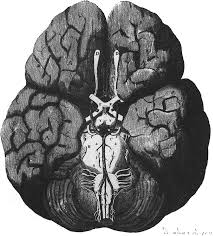
\includegraphics[width=\linewidth]{04_antecedentes/figures/thomas_willis.jpg}
    \end{minipage}
    \hfill
    \begin{minipage}{0.45\linewidth}
        \caption{
            El cerebro de Willis. Del libro \textit{Cerebri Anatome} \citep{willis1664cerebri}. 
            Este grabado representa las arterias cerebrales.
        }
        \label{fig:thomas_willis}
    \end{minipage}
\end{figure}

Esta ciencia ha experimentado transformaciones conceptuales profundas desde sus orígenes. Partiendo del debate entre visiones cardiocéntricas y encefalocéntricas, donde Aristóteles defendía una visión que situaba tanto el alma como las facultades cognitivas en el corazón, y por su parte, Hipócrates y, posteriormente Galeno, argumentaron que el cerebro era la base de la inteligencia y las emociones. Este debate, iniciado en la Grecia clásica encontró su resolución gradual a través de siglos de investigación anatómica y fisiológica \citep{blanco2014historia}.

Este conflicto entre visiones cardiocéntricas y encefalocentristas se mantuvo durante siglos. Galeno de Pérgamo (129-216 d.C.), a través de sus estudios anatómicos en animales, estableció una doctrina que dominaría el pensamiento médico durante más de un milenio: la teoría ventricular. Según esta concepción, los ventrículos cerebrales, las cavidades llenas de líquido en el interior del cerebro, eran los repositorios de las facultades mentales, organizadas jerárquicamente desde la sensación hasta la memoria y el razonamiento \citep{blanco2014historia}.

El siglo XVIII trajo consigo el descubrimiento de la naturaleza eléctrica de la actividad nerviosa, punto que analizaremos y trabajaremos mas adelante, un hallazgo que transformaría para siempre nuestra comprensión del sistema nervioso. Luigi Galvani (1737-1798) demostró en 1791 que la estimulación eléctrica podía provocar contracciones musculares gracias a sus experimentos en ranas, estableciendo que la ``electricidad animal'' era el medio de comunicación nerviosa \citep{blanco2014historia}. Este descubrimiento abrió la puerta a una comprensión del sistema nervioso basada en principios físicos mensurables.

Continuando con el siglo XIX el cual consolidó dos pilares fundamentales de la neurociencia moderna. Por un lado, Santiago Ramón y Cajal estableció la doctrina de la neurona, demostrando que el sistema nervioso está compuesto por células individuales discretas que se comunican a través de contactos especializados, posteriormente denominados sinapsis por Charles Sherrington. Por otro lado, los estudios sobre localización cortical de Paul Broca y Carl Wernicke establecieron que diferentes regiones cerebrales median funciones cognitivas específicas \citep{blanco2014historia}.

El siglo XX presenció avances decisivos para el presente trabajo. Alan Hodgkin y Andrew Huxley desarrollaron en la década de 1950 el primer modelo cuantitativo completo de la excitabilidad neuronal, describiendo los mecanismos iónicos del potencial de acción en el axón gigante del calamar \citep{hodgkin1952quantitative}. Este modelo, que les valió el Premio Nobel de Medicina en 1963, sigue siendo una referencia en la neurociencia computacional y será detallado en la Sección~\ref{subsec:Hodgkin-Huxley}.

\begin{figure}[H]
    \centering
    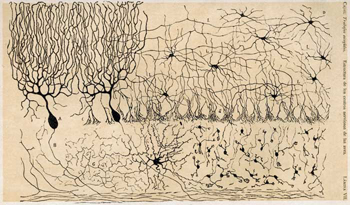
\includegraphics[width=0.55\textwidth]{04_antecedentes/figures/CajalCerebellum.jpg}
    \caption{
        Dibujo de Ramón y Cajal de las células del cerebelo de un pollo, mostrado en ``Estructura de los centros nerviosos de las aves'', Madrid, 1905.
    }
    \label{fig:cajal-cerebelo}
\end{figure}

Complementariamente, los estudios de Henry Dale, Otto Loewi y Bernard Katz establecieron los principios de la transmisión sináptica química, revelando cómo los neurotransmisores median la comunicación entre neuronas \citep{blanco2014historia}. Y finalmente, David Hubel y Torsten Wiesel revolucionaron nuestra comprensión del procesamiento visual cortical en las décadas de 1950 y 1960. Mediante registros electrofisiológicos en la corteza visual de gatos, descubrieron que las neuronas corticales responden selectivamente a características específicas del estímulo, como la orientación de barras luminosas \citep{hubel1959receptive}. Describieron la organización jerárquica del sistema visual, desde células simples que responden a bordes orientados en posiciones específicas, hasta células complejas con mayor invariancia espacial. Su trabajo, reconocido con el Premio Nobel de Medicina en 1981, estableció los principios de selectividad neuronal que fundamentan los modelos computacionales de corteza visual, incluyendo el modelo de \citet{echeveste2020cortical} que implementaremos en este trabajo.

Estos desarrollos históricos convergieron con el nacimiento de las ciencias de la computación para dar lugar a la neurociencia computacional, disciplina que proporciona el marco teórico y metodológico del presente trabajo.

% =============================================================================
% SECCIÓN 2: FUNDAMENTOS BIOLÓGICOS (CITAS CORREGIDAS)
% =============================================================================

\section{Fundamentos biológicos}
\label{sec:fundamentos_biologicos}

Los modelos computacionales de procesamiento neuronal deben fundamentarse en las propiedades biológicas de las neuronas y los circuitos que las interconectan. En esta sección vamos a presentar los principios biológicos esenciales que subyacen a los modelos estudiados en este trabajo, desde los mecanismos iónicos de la señalización neuronal hasta la organización funcional de las áreas corticales involucradas en la percepción visual y multisensorial.

\begin{figure}[H]
    \centering
    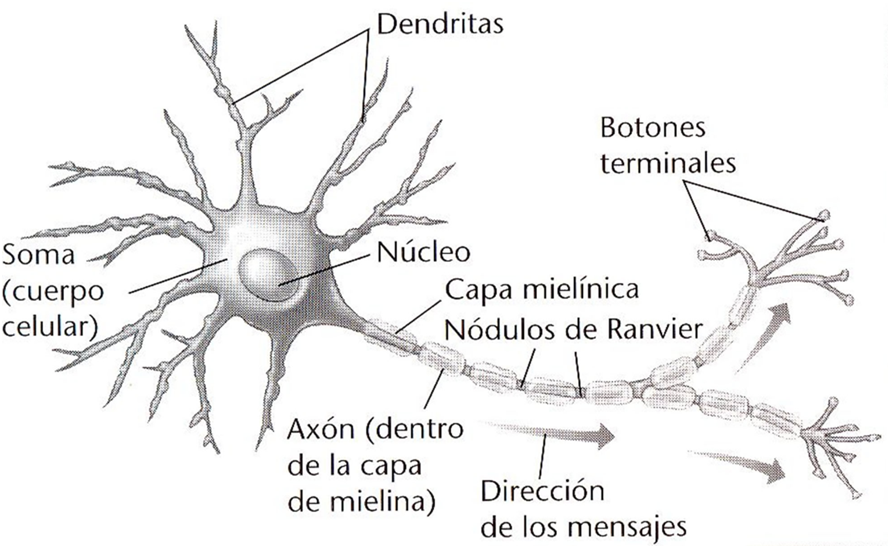
\includegraphics[width=0.65\textwidth]{04_antecedentes/figures/neurona.png}
        \caption{
        Estructura anatómica de una neurona, mostrando sus componentes principales.
    }
    \label{fig:neurona}
\end{figure}

\subsection{La neurona como unidad funcional}
\label{subsec:neurona_unidad}

La neurona es la unidad fundamental de procesamiento del sistema nervioso. Estructuralmente, cada neurona comprende un cuerpo celular o soma que contiene el núcleo y la maquinaria metabólica, dendritas que reciben señales de otras neuronas, un axón que transmite señales hacia células postsinápticas, y terminales sinápticos especializados para la liberación de neurotransmisores \citep{dayan2005theoretical}.

Toda esta estructura está delimitada por una membrana celular cuyas propiedades eléctricas son fundamentales para la comunicación entre neuronas, que depende de cambios rápidos en el potencial eléctrico. En reposo, esta membrana mantiene una diferencia de potencial de aproximadamente $-70$ mV, con el interior de la célula negativo respecto al exterior. Este potencial de reposo se establece mediante canales iónicos selectivos, principalmente permeables a iones de potasio (K$^+$), junto con la acción de bombas iónicas que mantienen los gradientes de concentración \citep{dayan2005theoretical}.

\subsubsection{Canales iónicos y potencial de acción}

Los canales iónicos son proteínas integrales que atraviesan la membrana celular y permiten el paso selectivo de iones específicos. La particularidad de los canales iónicos neuronales es su alta conductancia, del orden de $10^7$ cargas por segundo, lo que permite los cambios rápidos en el potencial de membrana necesarios para generar potenciales de acción \citep{dayan2005theoretical}.

El potencial de acción, descubierto y caracterizado cuantitativamente por \citet{hodgkin1952quantitative}, constituye la señal eléctrica fundamental mediante la cual las neuronas transmiten información a distancia. Su generación depende de dos poblaciones de canales iónicos dependientes de voltaje: los canales de sodio (Na$^+$), cuya apertura produce la despolarización rápida de la membrana, y los canales de potasio (K$^+$), cuya apertura más lenta permite la repolarización. El potencial de acción procede según un patrón de ``todo o nada'', donde todos los impulsos exhiben la misma amplitud, y la intensidad del estímulo se codifica mediante la frecuencia de disparo \citep{dayan2005theoretical}.

El modelo de Hodgkin-Huxley, que será presentado en detalle en la Sección~\ref{subsec:Hodgkin-Huxley}, formaliza matemáticamente estos mecanismos mediante un sistema de ecuaciones diferenciales que describe la dinámica del potencial de membrana en función de las conductancias iónicas dependientes de voltaje.

\begin{figure}[H]
    \centering
    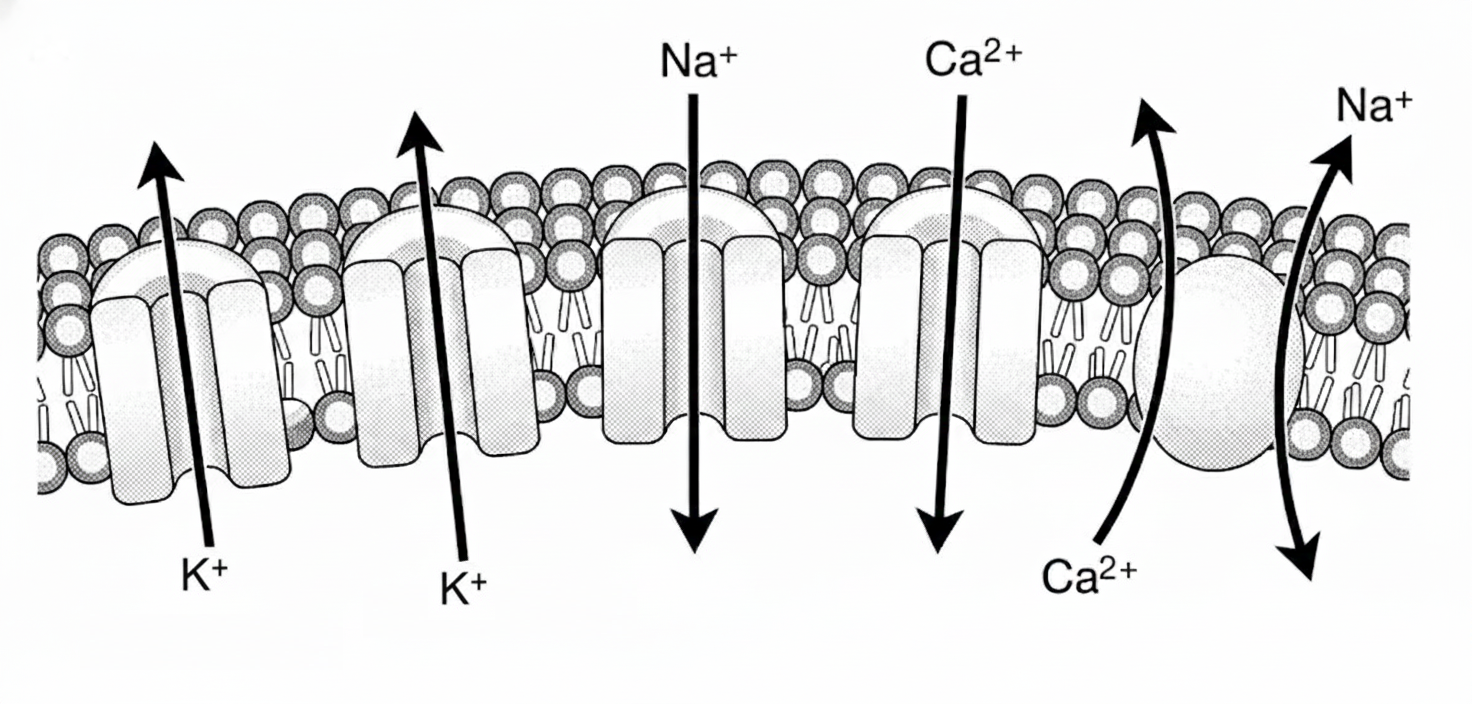
\includegraphics[width=0.75\textwidth]{04_antecedentes/figures/canal-ionico.png}
        \caption{
        Representación esquemática de la membrana neuronal mostrando canales iónicos selectivos.
    }
    \label{fig:canal-ionico}
\end{figure}

\subsubsection{Transmisión sináptica}

La comunicación entre neuronas ocurre predominantemente mediante sinapsis químicas, donde la llegada de un potencial de acción al terminal presináptico desencadena la liberación de neurotransmisores hacia la hendidura sináptica. Estos neurotransmisores se unen a receptores en la membrana de la neurona postsináptica, alterando su conductancia iónica y modificando su potencial eléctrico junto con la probabilidad de que esta genere su propio impulso\citep{dayan2005theoretical}.

Este mecanismo se modela como una transferencia de señales con efectos contrapuestos. Dependiendo del tipo de interacción, la neurona receptora puede sufrir una despolarización (excitación), que aumenta su probabilidad de disparo, o una hiperpolarización (inhibición), que la reduce. Esta distinción funcional permite organizar los modelos de redes neuronales, un tema que explicaremos más adelante en la Sección \ref{subsec:modelos_neuronas}.

\subsection{El sistema visual: de la retina a la corteza}
\label{subsec:sistema_visual}

El sistema visual procesa la información luminosa a través de una serie de estaciones organizadas jerárquicamente: retina, núcleo geniculado lateral del tálamo (LGN), corteza visual primaria (V1), y áreas corticales extraestriadas. En cada nivel aumenta la complejidad de las características extraídas del estímulo visual \citep{dayan2005theoretical}.

\begin{figure}[H]
    \centering
    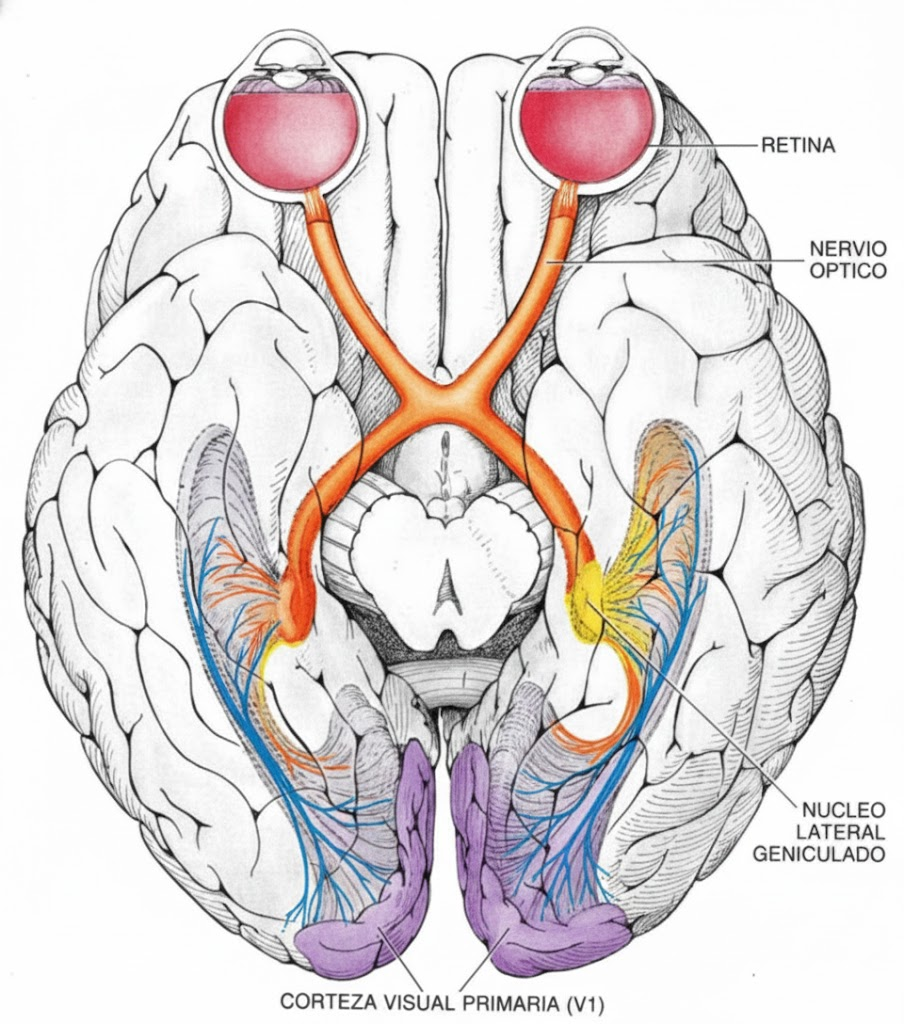
\includegraphics[width=0.65\textwidth]{04_antecedentes/figures/v1.jpg}
        \caption{
        Vía Visual Primaria. Esquema anatómico que muestra el sistema de transmisión de señales visuales.
    }
    \label{fig:patterns/v1}
\end{figure}

\subsubsection{Retina y células ganglionares}

La retina transforma la energía luminosa en señales eléctricas mediante los fotorreceptores: los conos, responsables de la visión en color y de alta resolución en condiciones de buena iluminación, y los bastones, más sensibles pero acromáticos, que permiten la visión en condiciones de baja luminosidad. Esta señal es procesada por circuitos locales antes de llegar a las células ganglionares cuyos axones forman el nervio óptico y constituyen la salida de la retina hacia el cerebro.

Dichas células ganglionares son un tipo de neuronas de axón mielinizado localizadas en la superficie interna de la retina. Se clasifican en dos tipos principales según su tamaño y propiedades funcionales: las células magnocelulares (M), grandes y sensibles al movimiento y contraste, y las células parvocelulares (P), más pequeñas y sensibles al color y detalle fino. Estas neuronas responden a estímulos lumínicos únicamente dentro de una región concreta del espacio visual denominada campo receptivo, y sus respuestas dependen del contraste entre regiones iluminadas y oscuras \citep{dayan2005theoretical}. Los campos receptivos de las células ganglionares presentan una organización centro-periferia antagonista: las células centro-ON se excitan con luz en el centro de su campo receptivo y se inhiben con luz en la periferia, mientras que las células centro-OFF presentan el patrón inverso. Esta distinción nos sera útil en los siguientes párrafos.

\subsubsection{Núcleo geniculado lateral}

El \acrfull{LGN}, localizado en el tálamo dorsal, constituye la principal estación de procesamiento y relevo entre la retina y la corteza visual primaria (V1). Actúa como un sofisticado filtro que organiza y modula el flujo de información en el marco de un procesamiento jerárquico.

Estructuralmente, el \acrshort{LGN} preserva de forma estricta la organización retinotópica y mantiene la segregación de las vías funcionales paralelas que emergen de la retina a través de una organización laminar especializada (capas físicas). Las capas magnocelulares (capas 1-2) reciben aferencias de las células ganglionares M, especializándose en la detección de movimiento y bajas frecuencias espaciales con una alta velocidad de conducción. Por su parte, las capas parvocelulares (capas 3-6) reciben información de las células P, procesando detalles finos y color (ejes rojo-verde). Entre estas capas se sitúan las zonas koniocelulares, que reciben información de las células K, vinculadas al procesamiento del espectro azul-amarillo \citep{dayan2005theoretical}.

Funcionalmente, las neuronas del \acrshort{LGN} presentan campos receptivos con una organización centro-periferia antagonista (células ON y OFF), similar a las células ganglionares de la retina. Sin embargo, la importancia de esta etapa reside en cómo dicha configuración facilita las transformaciones de orden superior en la jerarquía visual. La convergencia espacial de múltiples neuronas del \acrshort{LGN}, cuyos campos receptivos se alinean en el espacio visual, permite que las neuronas en la capa 4 de V1 desarrollen selectividad a la orientación de bordes, una característica inexistente en etapas previas.

Un aspecto crítico de su fisiología es la asimetría en sus conexiones: aunque el flujo principal de información visual es feedforward (Retina $\rightarrow$ LGN $\rightarrow$ V1), el \acrshort{LGN} recibe una cantidad significativamente mayor de conexiones feedback desde la corteza visual. Mientras que las señales de la retina actúan como ``conductores'' (\textit{drivers}) de la respuesta sensorial, las conexiones corticales feedback funcionan como ``moduladores''. Este sistema de retroalimentación permite que niveles jerárquicos superiores (V1) regulen la ganancia de contraste y ejecuten mecanismos de atención selectiva, filtrando activamente la información que debe ser transmitida a la corteza según las demandas de la tarea visual \citep{dayan2005theoretical}. Así, el \acrshort{LGN} se establece como la primera compuerta talamocortical donde el contexto y la predicción comienzan a dar forma a la percepción sensorial.

\subsubsection{Corteza visual primaria (V1)}

La corteza visual primaria, también conocida como área V1 o corteza estriada, constituye la primera estación de procesamiento cortical de la información visual. Como toda la corteza cerebral, V1 se organiza en seis capas horizontales numeradas del 1 al 6 desde la superficie hacia el interior. Cada capa tiene una composición celular y patrones de conectividad característicos: la capa 4 recibe las entradas principales desde el LGN, mientras que otras capas procesan esta información y la transmiten a otras regiones corticales.

\citet{hubel1959receptive} descubrieron que las neuronas de V1 responden selectivamente a características específicas de los estímulos, particularmente a bordes y barras con orientaciones determinadas, una propiedad ausente en las células ganglionares y del \acrshort{LGN}. A su vez, identificaron dos tipos principales de neuronas en V1. Las \textit{células simples}, ubicadas principalmente en la capa 4, presentan campos receptivos con regiones ON y OFF separadas espacialmente, respondiendo a bordes orientados en posiciones específicas del campo visual. Cada célula simple está afinada para detectar estímulos con orientaciones en un rango de aproximadamente diez grados \citep{blanco2014historia}. Y las \textit{células complejas}, localizadas en las capas 2, 3, 5 y 6, responden también a bordes orientados pero con mayor invariancia a la posición exacta del estímulo dentro de su campo receptivo, que es más amplio que el de las células simples. El modelo de Hubel y Wiesel propone que la selectividad a orientación de las células simples surge de la convergencia de entradas desde células del LGN con campos receptivos alineados \citep{dayan2005theoretical}.

En V1, las neuronas con propiedades de respuesta similares se organizan en columnas verticales que atraviesan las diferentes capas corticales. Las columnas de orientación, de entre 30 y 100 micrómetros de grosor, agrupan neuronas que responden a la misma orientación preferida. Estas columnas se disponen sistemáticamente de modo que un recorrido tangencial a través de la corteza encuentra secuencialmente todas las orientaciones posibles. Las columnas de dominancia ocular alternan el predominio de respuesta al ojo izquierdo y derecho. El conjunto de columnas que representa un ciclo completo de orientaciones para ambos ojos, junto con las estructuras denominadas ``blobs'' que procesan información de color, constituye una \textit{hipercolumna} de aproximadamente un milímetro cuadrado \citep{blanco2014historia, dayan2005theoretical}. Esta organización modular se repite a lo largo de toda la superficie de V1.

Esta arquitectura columnar es directamente relevante para el modelo de Echeveste, que simula precisamente una hipercolumna de V1 como unidad funcional para la inferencia probabilística sobre orientaciones visuales, como se detallará en el Capítulo~\ref{chapter:modelos_estudiados}.

\begin{figure}[H]
    \centering
    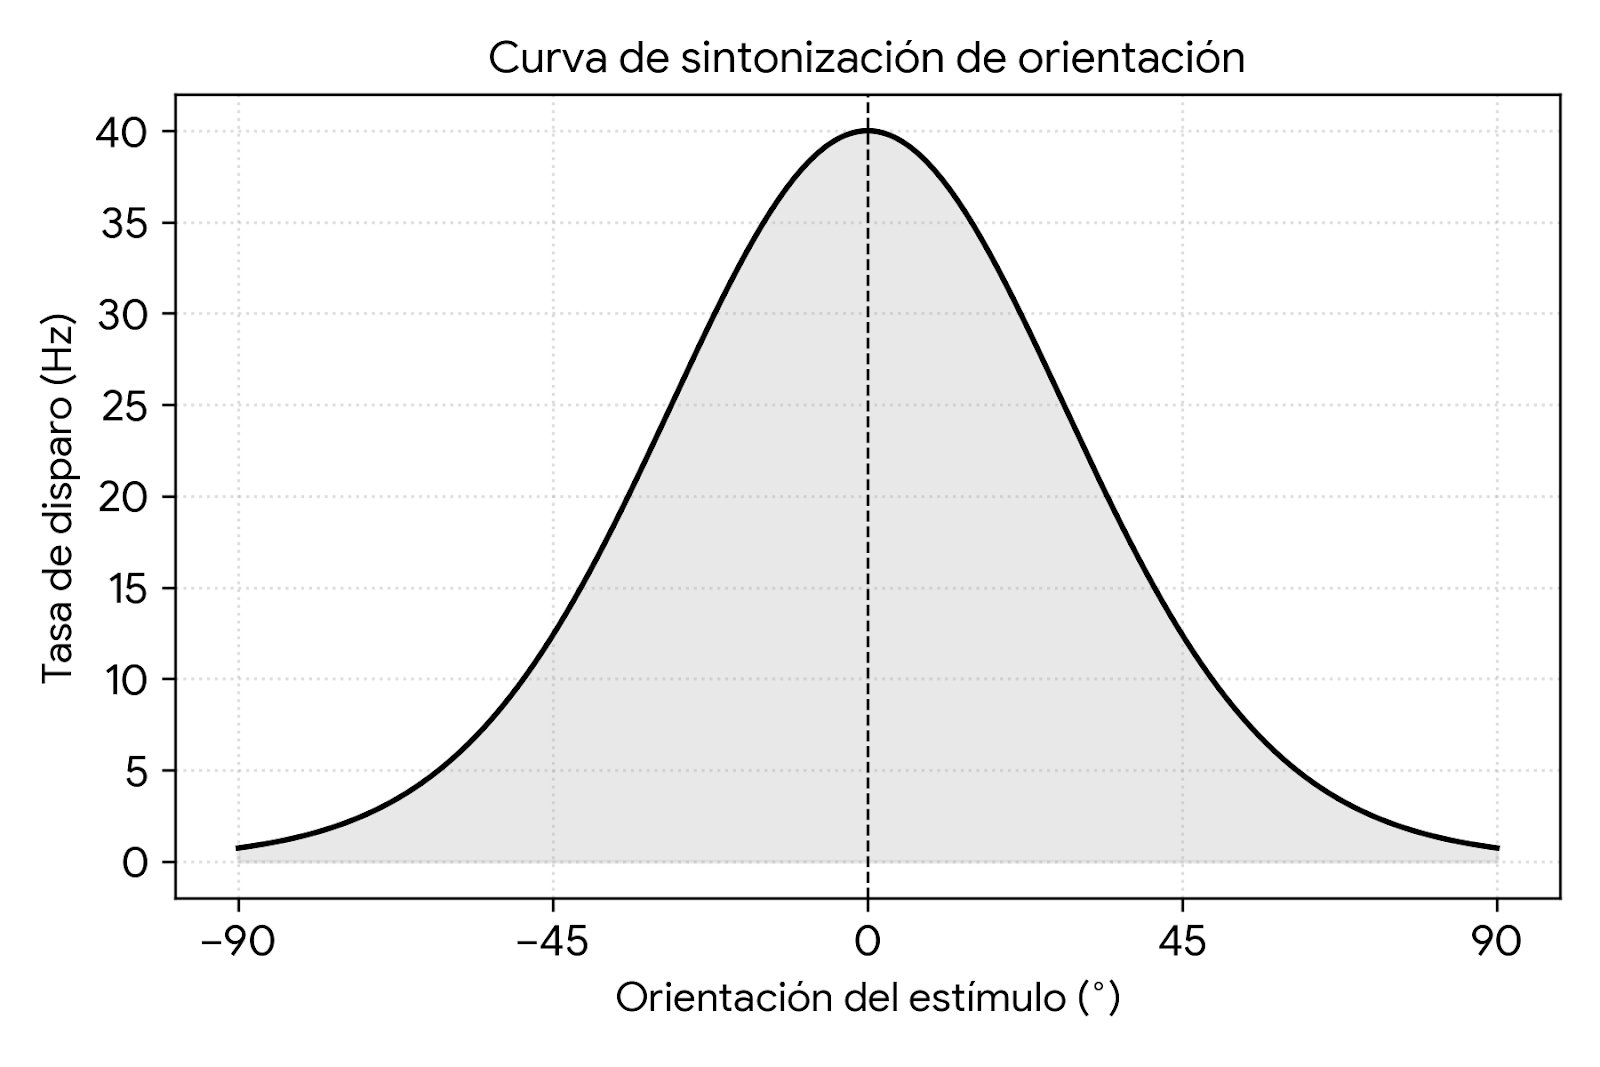
\includegraphics[width=0.85\textwidth]{04_antecedentes/figures/tuning-curbe.png}
    \caption{
    Curva de sintonización (tuning curve) de orientación de una neurona en V1. La respuesta (tasa de disparo en Hz) es máxima ante una orientación específica del estímulo y decrece conforme la inclinación del borde se desvía de la preferencia de la neurona.
    }
    \label{fig:tuning-curbe}
\end{figure}

\subsection{Filtros de Gabor como modelo de campos receptivos}
\label{subsec:filtros_gabor}

Los campos receptivos de las células simples de V1, con sus regiones ON y OFF, pueden aproximarse matemáticamente. Una función de Gabor es el producto de una función gaussiana, que define la extensión espacial del campo receptivo, y una función sinusoidal, que captura la estructura de bandas claras y oscuras \citep{dayan2005theoretical}:

\begin{equation}
D_s(x, y) = \frac{1}{2\pi\sigma_x\sigma_y} \exp\left(-\frac{x^2}{2\sigma_x^2} - \frac{y^2}{2\sigma_y^2}\right) \cos(kx - \phi)
\label{eq:gabor_function}
\end{equation}

Los parámetros de esta función determinan las propiedades del campo receptivo: $\sigma_x$ y $\sigma_y$ controlan la extensión espacial en las direcciones horizontal y vertical respectivamente, $k$ es la frecuencia espacial preferida que determina el espaciado entre bandas claras y oscuras, y $\phi$ es la fase espacial preferida que determina dónde caen los límites entre regiones ON y OFF dentro del campo receptivo. Estudios experimentales han demostrado que las funciones de Gabor proporcionan excelentes aproximaciones a los campos receptivos medidos en células simples de la corteza visual de gatos y primates \citep{dayan2005theoretical}.

La orientación preferida de un filtro de Gabor se obtiene rotando el sistema de coordenadas. Y finalmente una neurona con orientación preferida $\theta$, responde máximamente a bordes orientados en dicha dirección. Estos filtros juegan un papel central en el \acrfull{GSM} utilizado por \citet{echeveste2020cortical} el cual se explicará en el Capítulo \ref{chapter:modelos_estudiados}. 

\begin{figure}[H]
    \centering
    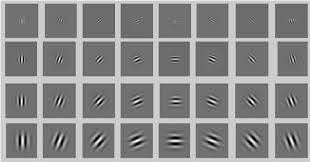
\includegraphics[width=0.75\textwidth]{04_antecedentes/figures/gabor-bank.jpg}
    \caption{
    Banco de filtros de Gabor utilizados para modelar los campos receptivos de las células simples en V1. Cada subfigura representa un filtro con una combinación específica de orientación ($\theta$) y frecuencia espacial ($k$). La extensión espacial de cada campo receptivo está dada por $\sigma_x$ y $\sigma_y$ en la Ecuación~\ref{eq:gabor_function}.
    }
    \label{fig:gabor-banks}
\end{figure}

\subsection{Vías visuales: procesamiento paralelo}
\label{subsec:vias_visuales}

Después del procesamiento inicial en V1, la información visual se distribuye a través de múltiples áreas corticales extraestriadas organizadas en dos corrientes principales de procesamiento paralelo \citep{dayan2005theoretical}:

\textbf{La vía ventral} se proyecta desde V1 hacia V2, V4 y la corteza inferotemporal. Esta vía se especializa en el reconocimiento de objetos, procesando información sobre forma, color e identidad. Lesiones en esta vía producen agnosias visuales, dificultades para reconocer objetos a pesar de una visión básica preservada.

\textbf{La vía dorsal} se proyecta desde V1 hacia V2, el área MT (V5) y la corteza parietal posterior. Esta vía procesa información sobre movimiento, localización espacial y guía de acciones motoras. Lesiones en esta vía producen déficits en la localización de objetos y en la coordinación visomotora.

Esta división funcional tiene implicaciones directas para los modelos que estudiaremos. El modelo de Echeveste, que representa características visuales como la orientación en una hipercolumna de V1, está más relacionado con el procesamiento de la vía ventral. En contraste, el modelo de Cuppini, que representa la localización espacial de estímulos audiovisuales, está más relacionado con el procesamiento de la vía dorsal. Como se discutirá en el Capítulo~\ref{chapter:modelos_estudiados}, la eventual integración de ambos enfoques requerirá considerar cómo interactúan estos diferentes tipos de representaciones corticales.

\subsection{El colículo superior y la integración multisensorial}
\label{subsec:coliculo_superior}

El \acrfull{CS} es una estructura del mesencéfalo que desempeña un papel fundamental en la orientación de la atención y los movimientos oculares hacia estímulos relevantes del entorno. A diferencia de las áreas corticales discutidas anteriormente, el \acrshort{CS} recibe información de múltiples modalidades sensoriales, visual, auditiva y somatosensorial, organizándolas en mapas topográficos superpuestos \citep{stein2012new}.

El \acrshort{CS} se organiza en capas funcionalmente diferenciadas: las capas superficiales procesan predominantemente información visual y mantienen una representación retinotópica del campo visual, mientras que las capas profundas son multimodales y contienen neuronas que responden a estímulos de diferentes modalidades cuando estos provienen de ubicaciones espaciales coincidentes. Esta convergencia anatómica de información multisensorial hace del \acrshort{CS} un punto ideal para estudiar los mecanismos de integración sensorial.

Estudios electrofisiológicos en el \acrshort{CS} han revelado principios fundamentales de la integración multisensorial que los modelos computacionales deben capturar \citep{stein2012new, paredes2025scikit}. La \textit{regla espacial} establece que estímulos de diferentes modalidades cercanos en el espacio producen respuestas potenciadas (superaditivas) comparadas con las respuestas unimodales, mientras que estímulos distantes producen respuestas deprimidas. La \textit{regla temporal} indica que la integración es máxima cuando los estímulos de diferentes modalidades son cercanos en el tiempo. Y la \textit{regla de efectividad inversa} establece que la potenciación multisensorial es mayor cuando los estímulos unimodales individuales son débiles o ambiguos \citep{cuppini2017biologically}.

El modelo de Cuppini, que será presentado en el Capítulo~\ref{chapter:modelos_estudiados}, captura estos principios mediante una arquitectura de tres capas donde las regiones unisensoriales están organizadas topográficamente y conectadas a una capa de inferencia causal que determina si estímulos audiovisuales provienen de una fuente común o de fuentes independientes.

\subsection{De la biología a la computación}
\label{subsec:sintesis_biologia}

Los fundamentos biológicos presentados en esta sección establecen las restricciones y fenómenos que los modelos computacionales de procesamiento neuronal deben capturar. La organización jerárquica del sistema visual, desde los campos receptivos en la retina hasta la selectividad a orientación en V1, proporciona el sustrato para el modelo de Echeveste. A su vez, la integración multisensorial en estructuras como el colículo superior, con sus principios de coincidencia espacial y temporal, fundamenta el modelo de Cuppini.

Ya desarrolladas las restricciones biológicas fundamentales. La siguiente sección presenta el marco formal de la neurociencia computacional que permite formalizar estas restricciones y evaluar las capacidades de los modelos resultantes.

% =============================================================================
% SECCIÓN 2: NEUROCIENCIA COMPUTACIONAL
% =============================================================================

\section{Neurociencia computacional}
\label{sec:neuro_computacional}

La neurociencia computacional representa una síntesis moderna de neurobiología, matemáticas y ciencias de la computación, orientada a comprender cómo el sistema nervioso procesa información y genera comportamiento. Esta disciplina no se limita a simular fenómenos neuronales, también busca identificar los principios computacionales fundamentales que subyacen a las funciones cerebrales y estudiar como estos métodos matemáticos, físicos e informáticos pueden proporcionar información importante sobre el funcionamiento del sistema nervioso \citep{dayan2005theoretical}.

\subsection{Los tres niveles}
\label{subsec:marr_niveles}

Un marco conceptual fundamental para la neurociencia computacional fue propuesto por \citet{marr2010vision} en su influyente obra \textit{Vision}. Donde argumentó que cualquier sistema de procesamiento de información puede ser analizado en tres niveles distintos, pero complementarios \citep{marr2010vision}:

El \textbf{nivel computacional} aborda la pregunta de \textit{qué} computa el sistema y \textit{por qué}. En este nivel, se especifica el problema computacional que el sistema debe resolver y la lógica de la estrategia mediante la cual puede resolverse. Por ejemplo, para la corteza visual, el problema computacional podría ser inferir las características más probables de un estímulo (como su orientación o contraste) a partir de información sensorial ruidosa, representando no solo una estimación puntual, sino la incertidumbre asociada a dicha estimación.

El \textbf{nivel algorítmico} pregunta \textit{cómo} se lleva a cabo ese cómputo, sin comprometerse todavía con el sustrato físico que lo ejecuta. ¿Qué representaciones utiliza el sistema? ¿Qué algoritmos transforman estas representaciones? Este nivel especifica los procedimientos concretos mediante los cuales se resuelve el problema computacional.

Finalmente, el \textbf{nivel de implementación} se ocupa de cómo los circuitos neuronales implementan el algoritmo. ¿Qué circuitos neuronales realizan el cómputo? ¿Cómo se codifica la información en patrones de actividad neuronal? Por ejemplo, en el caso de la inferencia probabilística, esto implica especificar cómo redes recurrentes de neuronas, pueden implementar el muestreo de distribuciones posteriores.

Esta jerarquía de niveles proporciona una estructura para organizar nuestro conocimiento del cerebro y, específicamente, para conectar descripciones funcionales con mecanismos neuronales. En este trabajo, donde buscamos implementar un modelo de inferencia causal multisensorial con dinámicas corticales realistas, se opera precisamente en la interfaz entre estos niveles: partimos de una especificación computacional (inferencia bayesiana) y buscamos su implementación en circuitos neuronales biológicamente plausibles.

\subsection{Codificación y decodificación neuronal}
\label{subsec:codificacion_neuronal}

Una cuestión central en neurociencia computacional es cómo las neuronas representan información sobre el mundo externo y los estados internos del organismo. La investigación en este ámbito se ha centrado en dos problemas complementarios: la \textit{codificación neuronal} (cómo los estímulos se traducen en patrones de actividad neuronal) y la \textit{decodificación neuronal} (cómo la información puede extraerse de estos patrones) \citep{dayan2005theoretical}.

El patrón neuronal más estudiado tradicionalmente es la \textbf{tasa de disparo}: la frecuencia promedio de potenciales de acción generados por una neurona en un intervalo de tiempo dado. Estudios clásicos de Adrian en la década de 1920 demostraron que la intensidad de un estímulo se correlaciona con la tasa de disparo de las neuronas sensoriales \citep{blanco2014historia}. Sin embargo, trabajos recientes han propuesto que el \textbf{potencial de membrana} en sí mismo puede servir como variable representacional. En este enfoque, no solo el valor medio del potencial sino también su variabilidad codifica información relevante sobre el estímulo y la incertidumbre asociada a su estimación. La tasa de disparo se deriva entonces como una transformación no lineal del potencial de membrana.

Esta relación entre potencial de membrana y tasa de disparo tiene implicaciones importantes para la codificación poblacional. Cuando múltiples neuronas representan conjuntamente un estímulo, la distribución de sus potenciales de membrana puede codificar no solo una estimación puntual de las características del estímulo, sino toda una distribución de probabilidad que refleja la incertidumbre perceptual. Por todo esto, la elección de cómo modelar la dinámica neuronal determina qué tipo de información puede ser codificada y posteriormente decodificada del patrón de actividad poblacional. En la Sección~\ref{sec:modelo_echeveste} exploraremos en detalle cómo esta idea se formaliza matemáticamente en el contexto de la inferencia probabilística.

\subsection{Modelos de neuronas}
\label{subsec:modelos_neuronas}

La neurociencia computacional ha desarrollado una variedad de modelos de neuronas con diferentes niveles de detalle biofísico, desde descripciones detalladas que involucran miles de ecuaciones diferenciales acopladas hasta simplificaciones útiles para estudiar grandes redes interconectadas. La elección del modelo apropiado depende de las preguntas que se desean abordar y del compromiso entre realismo biológico y tratabilidad computacional \citep{dayan2005theoretical}.

\subsubsection{El modelo de Hodgkin-Huxley}
\label{subsec:Hodgkin-Huxley}

El modelo Hodgkin-Huxley constituye una de las bases del modelado biofísico de neuronas \citep{hodgkin1952quantitative}. Desarrollado a partir de experimentos en el axón gigante del calamar, este modelo describe cómo los potenciales de acción surgen de la apertura y cierre de canales iónicos dependientes de voltaje. El modelo integra propiedades eléctricas fundamentales de la membrana neuronal: la capacitancia de membrana $C_m$, las conductancias de los canales de sodio, potasio y fuga ($\bar{g}_{Na}$, $\bar{g}_K$ y $g_L$), y la actividad de las puertas iónicas descrita por las variables $m$, $h$ y $n$, que se abren y cierran con tasas dependientes del voltaje. Estas propiedades se relacionan mediante un sistema de cuatro ecuaciones diferenciales acopladas, cuya ecuación principal describe la dinámica del potencial de membrana $V$:
\begin{equation}
C_m \frac{dV}{dt} = -\bar{g}_{Na}m^3h(V-E_{Na}) - \bar{g}_K n^4(V-E_K) - g_{L}(V-E_{L}) + I_{ext}
\label{eq:hodgkin_huxley}
\end{equation}
El modelo captura cuantitativamente la generación del potencial de acción, incluyendo su forma característica y el período refractario \citep{dayan2005theoretical}. Sin embargo, su complejidad computacional lo hace impráctico para simulaciones de redes grandes.

\subsubsection{El modelo integra-y-dispara}

Para simulaciones a mayor escala, se emplean modelos simplificados que capturan las características esenciales de la dinámica neuronal. El modelo integra y dispara (\ac{LIF}) es quizás el más ampliamente utilizado. Según \cite{eliasmith2003neural}, este modelo representa un balance conveniente entre realismo neuronal y tratabilidad computacional ya que introduce la no linealidad más prominente de los sistemas neuronales, el potencial de acción, mientras mantiene una formulación matemática simple:

\begin{equation}
\tau_m \frac{dV}{dt} = -(V - V_{rest}) + R_m I(t)
\label{eq:lif}
\end{equation}
donde $V$ es el potencial de membrana, $\tau_m$ es la constante de tiempo de membrana, $V_{rest}$ es el potencial de reposo, $R_m$ es la resistencia de membrana, e $I(t)$ es la corriente de entrada. Cuando $V$ alcanza un umbral $V_{th}$, se registra un potencial de acción y el potencial se reinicia a un valor $V_{reset}$.

A pesar de su simplicidad, el modelo LIF reproduce muchas propiedades cualitativas de neuronas reales, incluyendo la variabilidad en los tiempos de disparo y la sensibilidad a fluctuaciones en la entrada \citep{dayan2005theoretical}.

\begin{figure}[H]
    \centering
    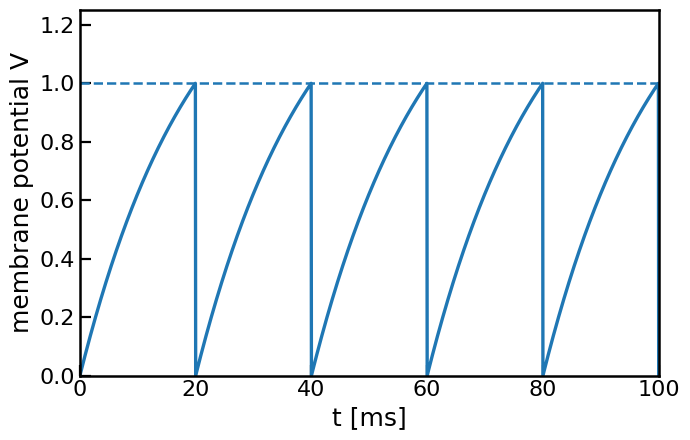
\includegraphics[width=0.55\textwidth]{04_antecedentes/figures/integrate_fire.png}
    \caption{
        Evolución temporal del potencial de membrana $V$ de una neurona \textit{integra-y-dispara} impulsada por una corriente constante. Para mayor claridad, el potencial se presenta normalizado respecto al umbral de disparo ($V_{th} = 1.0$) y el reposo ($V_{reset} = 0$).
    }
    \label{fig:integrate_fire}
\end{figure}

\subsubsection{Modelos de tasa}

En un nivel aún más abstracto, los \textbf{modelos de tasa} (\textit{rate models}) describen la actividad neuronal en términos de la tasa de disparo promedio de poblaciones de neuronas, ignorando los tiempos precisos de los potenciales de acción individuales \citep{dayan2005theoretical}. Una formulación común es:

\begin{equation}
\tau \frac{dr}{dt} = -r + f\left(\sum_j w_{ij} r_j + h_i\right)
\label{eq:rate_model}
\end{equation}

donde $r$ es la tasa de disparo, $f(\cdot)$ es una función de transferencia no lineal (típicamente sigmoide o rectificadora), $w_{ij}$ son los pesos sinápticos, y $h_i$ es la entrada externa.

Los modelos de tasa son computacionalmente eficientes y han sido ampliamente utilizados para estudiar fenómenos como la memoria de trabajo, la toma de decisiones, y la integración sensorial. Sin embargo, al promediar la actividad neuronal, no capturan la variabilidad temporal que caracteriza la actividad cortical real \citep{gerstner2002spiking}.

\subsubsection{Neuronas estocásticas con dinámica de membrana}

El modelo neuronal propuesto por \cite{echeveste2020cortical}, el cual es el objeto de estudio de este trabajo, ocupa un lugar intermedio en la jerarquía de complejidad presentada. A diferencia de los modelos de tasa puros, este enfoque mantiene el potencial de membrana como variable dinámica principal, permitiendo que su variabilidad temporal codifique información. A diferencia del modelo LIF, no implementa un mecanismo de disparo explícito con umbral y reinicio, sino que deriva la tasa de disparo como una transformación continua y supralineal del potencial de membrana.

Crucialmente, este tipo de modelo incorpora dos características biológicas fundamentales: ruido estocástico que genera variabilidad en las respuestas, y la distinción explícita entre poblaciones excitatorias e inhibitorias, respetando el principio de Dale (cada neurona libera el mismo tipo de neurotransmisor en todas sus sinapsis, siendo exclusivamente excitatoria o inhibitoria). Estas características resultan esenciales para implementar inferencia probabilística mediante muestreo, como se desarrollará en profundidad en la Sección~\ref{sec:modelo_echeveste}.

En síntesis, los modelos presentados representan diferentes compromisos entre fidelidad biofísica y tratabilidad computacional. Sin embargo, las propiedades computacionales de estos modelos dependen no solo de la dinámica de neuronas individuales, sino fundamentalmente de cómo estas se conectan formando redes. En la siguiente sección exploraremos cómo la arquitectura de conexiones recurrentes entre poblaciones excitatorias e inhibitorias da lugar a dinámicas corticales complejas.

\subsection{Conexiones neuronales}
\label{subsec:conexiones_neuronales}

Los modelos de neuronas individuales descritos anteriormente constituyen los bloques fundamentales del procesamiento neuronal. Sin embargo, las funciones cognitivas emergen de la interacción coordinada de miles o millones de neuronas conectadas en redes. La arquitectura de red, forma en que estas neuronas se conectan, determina en gran medida las capacidades computacionales del circuito. Según \cite{dayan2005theoretical}, existen tres clases principales de interconexiones en los circuitos neuronales.

Las \textbf{conexiones feedforward} traen información desde una región ubicada en una etapa anterior de procesamiento hacia una etapa posterior. Computacionalmente, las redes feedforward llamadas así por implementar solo este tipo de conexiones, implementan transformaciones jerárquicas donde cada capa extrae características progresivamente más abstractas de la entrada. Esta arquitectura es eficiente para tareas de clasificación y reconocimiento de patrones, y ha inspirado modelos exitosos como las redes convolucionales en aprendizaje profundo \citep{heaton2018ian}. Sin embargo, las redes puramente feedforward tienen limitaciones importantes: no pueden mantener información en ausencia de entrada, ni generar dinámicas temporales complejas.

\begin{figure}[H]
    \centering
    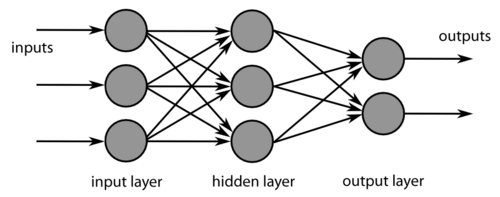
\includegraphics[width=0.55\textwidth]{04_antecedentes/figures/feed-forward.png}
    \caption{
        Modelo computacional de red neuronal feed-forward de una sola capa oculta.
    }
    \label{fig:feed-forward}
\end{figure}

Las \textbf{conexiones feedback} llevan señales de regreso desde etapas posteriores del procesamiento hacia etapas anteriores. El número de fibras feedforward y feedback entre regiones conectadas es típicamente comparable \citep{dayan2005theoretical}. Computacionalmente, estas conexiones permiten que información contextual y expectativas de niveles superiores modulen el procesamiento en niveles inferiores, implementando mecanismos como atención selectiva y codificación predictiva.

\begin{figure}[H]
    \centering
    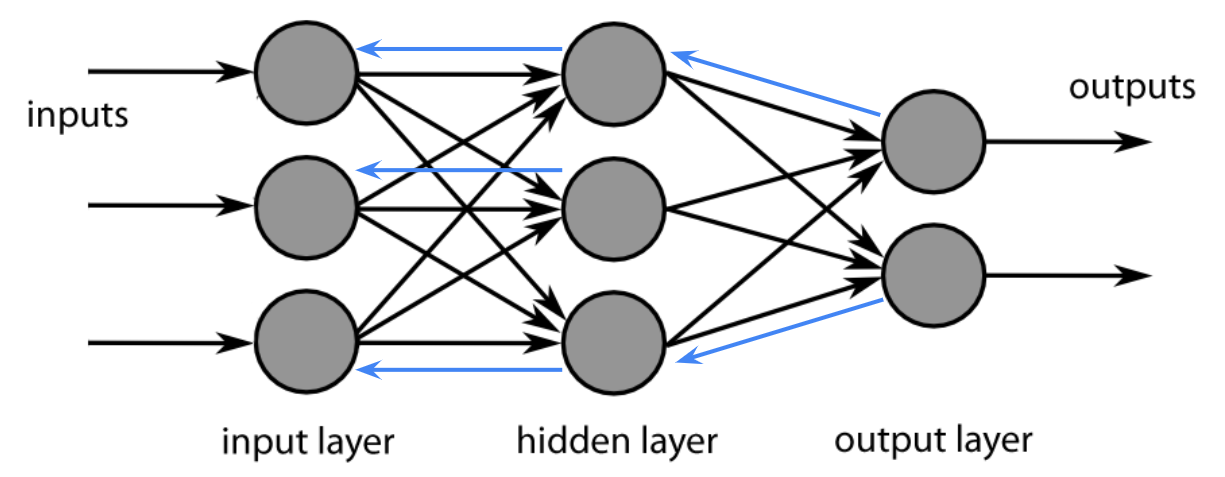
\includegraphics[width=0.55\textwidth]{04_antecedentes/figures/top-down.png}
    \caption{
    Arquitectura de red neuronal con conexiones feedforward e incluyendo conexiones feedback resaltadas en azul.
    }
    \label{fig:top-down}
\end{figure}

Las \textbf{conexiones recurrentes} interconectan neuronas dentro de una misma etapa de procesamiento. Una observación fundamental es que las sinapsis recurrentes típicamente superan en número a las conexiones feedforward o feedback \citep{dayan2005theoretical}. Esta preponderancia tiene profundas implicaciones computacionales: mientras que las redes feedforward transforman la información de manera estática, las redes con conectividad recurrente pueden generar dinámicas temporales complejas. Entre las capacidades únicas de las redes recurrentes se encuentran: \textbf{actividad sostenida} en ausencia de entrada externa, \textbf{amplificación selectiva} de señales débiles, \textbf{fenómenos oscilatorios} en diversas bandas de frecuencia, y formación de \textbf{estados atractores} que pueden servir como memorias asociativas \citep{dayan2005theoretical}.

Dada la importancia de la conectividad recurrente para las funciones computacionales que nos interesan en este trabajo, en la siguiente sección exploraremos en detalle las propiedades de las redes recurrentes y las dinámicas que emergen de ellas.

\begin{figure}[H]
    \centering
    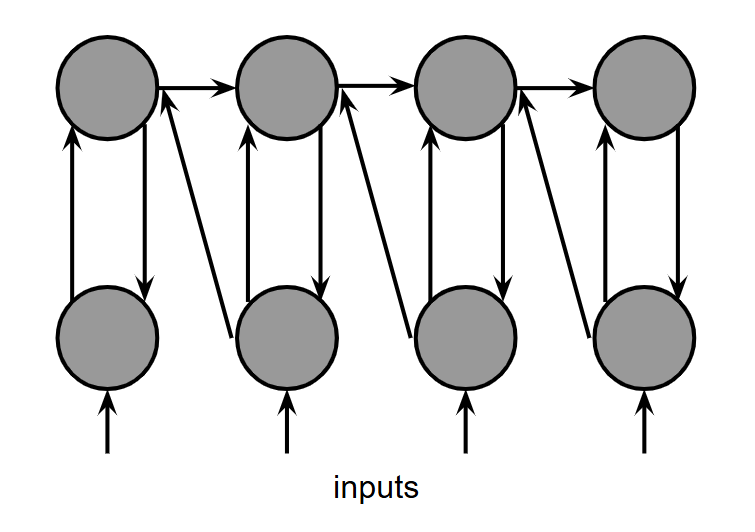
\includegraphics[width=0.5\textwidth]{04_antecedentes/figures/red-recurrente.png}
    \caption{
    Arquitectura de red recurrente. Las conexiones horizontales entre neuronas de la misma capa y las conexiones bidireccionales entre capas permiten que la actividad de cada neurona influya sobre sus vecinas, generando dinámicas temporales complejas.
    }
    \label{fig:red-recurrente}
\end{figure}

\subsection{Redes neuronales recurrentes y dinámicas corticales}
\label{subsec:redes_recurrentes}

Los circuitos corticales se caracterizan por conexiones recurrentes abundantes que pueden clasificarse según su efecto sobre la neurona postsináptica: las \textbf{conexiones excitatorias} aumentan el potencial de membrana, incrementando la probabilidad de disparo, mientras que las \textbf{conexiones inhibitorias} lo disminuyen, reduciendo dicha probabilidad. En el contexto del modelado computacional, esta distinción suele formalizarse mediante el \textbf{principio de Dale}, que asume que cada neurona libera el mismo tipo de neurotransmisor en todas sus sinapsis, clasificándose como excitatoria o inhibitoria. Si bien la evidencia actual muestra que las neuronas biológicas pueden co-liberar múltiples neurotransmisores, esta simplificación resulta útil para construir modelos tratables computacionalmente \citep{dale1935pharmacology}.

La interacción entre poblaciones excitatorias e inhibitorias da lugar a dinámicas complejas que van más allá de la simple transmisión de información feedforward \citep{dayan2005theoretical}. Como se mencionó anteriormente, si las conexiones recurrentes son suficientemente fuertes, el patrón de actividad poblacional puede volverse parcialmente independiente de la estructura de la entrada, permitiendo que la red mantenga estados de actividad que proveen memoria de entradas previas.

Un fenómeno particularmente importante que emerge de las redes recurrentes son las \textbf{oscilaciones neuronales}. Las interacciones entre poblaciones excitatorias e inhibitorias pueden generar actividad oscilatoria en diversas bandas de frecuencia, incluyendo oscilaciones gamma (30-80 Hz) que han sido asociadas con el procesamiento sensorial y la atención \citep{echeveste2020cortical}. Estas oscilaciones no son simples fenómenos sino que pueden cumplir roles funcionales específicos en el procesamiento de información.

Un modelo particularmente influyente que captura estas propiedades es la \textbf{red supralineal estabilizada} (\acrshort{SSN}, \textit{Stabilized Supralinear Network}), que incorpora propiedades esenciales de los circuitos corticales. Este modelo incluye poblaciones separadas de neuronas excitatorias e inhibitorias, funciones de transferencia supralineales (expansivas) consistentes con observaciones experimentales en neuronas corticales, y conectividad recurrente que estabiliza la actividad del circuito \citep{echeveste2020cortical}.

El SSN reproduce fenómenos corticales importantes como la normalización divisiva (un cómputo canónico de circuitos corticales), las respuestas transitorias al inicio de estímulos, y las oscilaciones gamma cuya frecuencia aumenta con el contraste del estímulo. Crucialmente, este modelo constituye la base arquitectónica del trabajo de \cite{echeveste2020cortical}, quienes demostraron cómo extenderlo para implementar inferencia probabilística basada en muestreo. Los detalles matemáticos completos de esta extensión, incluyendo la dinámica neuronal, la función de transferencia supralineal, el rol del ruido estocástico, y cómo estas propiedades emergen del objetivo de muestreo, se presentan en la Sección~\ref{sec:modelo_echeveste}.

% =============================================================================
% SECCIÓN 3: INTEGRACIÓN MULTISENSORIAL
% =============================================================================

\section{Integración multisensorial}
\label{sec:integracion_multisensorial}

La percepción de los estímulos que nos rodean rara vez depende de una única modalidad sensorial. Cuando conversamos con alguien, integramos información visual de los movimientos de sus labios con las señales auditivas de su voz. Esta integración de información proveniente de múltiples sentidos, conocida como \textbf{integración multisensorial}, es un proceso neuronal fundamental que mejora nuestra capacidad para percibir y actuar en el mundo \citep{stein2012new}.

\subsection{La percepción como inferencia probabilística}
\label{subsec:percepcion_bayesiana}

La inferencia probabilística proporciona una solución al problema de formar percepciones al mezclar información parcial y ruidosa de múltiples fuentes, incluyendo diferentes señales sensoriales, modalidades y formas de memoria \citep{echeveste2020cortical}. Formalmente, esta fusión resulta en una \textbf{distribución posterior} que expresa la probabilidad de que características relevantes del entorno sean interpretadas de diferentes formas, dada la información disponible a través de los sentidos.

Dado que, por ejemplo, el sistema visual solo tiene acceso a los fotones absorbidos en la retina, la interpretación de los objetos requiere ir más allá de la información directamente disponible. El cerebro debe entonces \textit{inferir} las propiedades del mundo externo a partir de esta información sensorial comúnmente incompleta y ruidosa. El teorema de Bayes nos proporciona el marco formal para esta inferencia:

\begin{equation}
P(\mathbf{y}|\mathbf{x}) = \frac{P(\mathbf{x}|\mathbf{y})P(\mathbf{y})}{P(\mathbf{x})}
\label{eq:bayes_perception}
\end{equation}

donde $\mathbf{y}$ representa las variables del mundo que se desean inferir, $\mathbf{x}$ son las observaciones sensoriales, $P(\mathbf{x}|\mathbf{y})$ es la verosimilitud (la probabilidad de observar los datos sensoriales $\mathbf{x}$ dado un estado específico del mundo $\mathbf{y}$), $P(\mathbf{y})$ es el conocimiento previo sobre el mundo llamado probabilidad a priori, y $P(\mathbf{y}|\mathbf{x})$ es la distribución posterior que representa la creencia actualizada tras observar los datos sensoriales.

El denominador $P(\mathbf{x})$ es la probabilidad marginal de las observaciones y se obtiene integrando sobre todas las interpretaciones posibles del mundo, $P(\mathbf{x}) = \int P(\mathbf{x}|\mathbf{y})P(\mathbf{y})\, d\mathbf{y}$. Salvo en casos muy particulares esta integral no tiene solución cerrada, de modo que ningún sistema, biológico o artificial, puede evaluar la Ecuación~\ref{eq:bayes_perception} de forma exacta. Conviene entonces precisar en qué sentido decimos que el cerebro realiza inferencia bayesiana: no que aplique el teorema de manera explícita, sino que su comportamiento es consistente con el de un observador que aproxima esa distribución posterior. Cómo se construye tal aproximación es justamente el problema que aborda el modelo implementado en este trabajo, donde la red no calcula la integral sino que genera muestras de la posterior mediante su propia actividad, tal como se detalla en la Sección~\ref{subsec:echeveste_marco}.

Evidencia en diversos campos sugiere que el cerebro representa distribuciones posteriores al menos de manera aproximada \citep{echeveste2020cortical}. Esta perspectiva tiene implicaciones profundas: la variabilidad en las respuestas sensoriales no sería simplemente ``ruido'' a eliminar, sino que podría reflejar la incertidumbre inherente a la inferencia sobre el estado del mundo.

\subsection{Combinación óptima de señales}
\label{subsec:combinacion_optima}

Cuando múltiples modalidades sensoriales proporcionan información sobre una misma propiedad del entorno, surge la pregunta de cómo combinarlas de manera óptima. Un modelo influyente propone que el proceso de combinación de señales se asemeja a un \textbf{integrador de máxima verosimilitud} \citep{alais2004ventriloquist}.

En el contexto de la localización espacial audiovisual, si $\hat{S}_A$ y $\hat{S}_V$ representan las estimaciones unimodales auditiva y visual respectivamente, la estimación integrada óptima se obtiene como un promedio ponderado:

\begin{equation}
\hat{S}_{AV} = w_A \hat{S}_A + w_V \hat{S}_V
\label{eq:mle_integration}
\end{equation}

donde los pesos $w_A$ y $w_V$ son proporcionales a la \textbf{confiabilidad} (inversa de la varianza) de cada modalidad:

\begin{equation}
w_A = \frac{\sigma_V^2}{\sigma_A^2 + \sigma_V^2}, \quad w_V = \frac{\sigma_A^2}{\sigma_A^2 + \sigma_V^2}
\label{eq:reliability_weights}
\end{equation}

Cabe aclarar que las varianzas $\sigma_A^2$ y $\sigma_V^2$ no son un dato externo que el sistema reciba junto con los estímulos, sino que deben estimarse a partir de las propias señales sensoriales. En los modelos de código poblacional que veremos más adelante esta estimación no requiere un cálculo aparte, porque la confiabilidad de cada modalidad queda representada de forma implícita en la actividad de la población que la codifica: entradas más confiables producen respuestas más intensas y más concentradas, y eso basta para que la combinación resultante se aproxime a la ponderación de la Ecuación~\ref{eq:reliability_weights}.

Esta formulación captura una intuición fundamental: las señales más confiables (con menor varianza) reciben mayor peso en la estimación final. La visión, típicamente más precisa espacialmente que la audición, domina la percepción de localización cuando ambas modalidades están disponibles \citep{paredes2025scikit}.

\subsection{El problema de la inferencia causal}
\label{subsec:inferencia_causal}

Dicho modelo asume implícitamente que todas las señales provienen de una misma fuente. Sin embargo, en el mundo real, señales de diferentes modalidades pueden originarse de eventos independientes. Cuando existe una diferencia significativa entre las estimaciones $\hat{S}_A$ y $\hat{S}_V$, el observador enfrenta un cuestionamiento natural: ¿esta diferencia se debe a ruido en el procesamiento neural, o indica que las señales provienen de fuentes separadas? \citep{paredes2025scikit}.

El modelo de \textbf{inferencia causal bayesiana} \citep{kording2007causal} extiende el marco probabilístico para abordar este problema. El observador debe inferir no solo la localización de los estímulos, sino también la \textit{estructura causal} subyacente: si las señales auditiva y visual provienen de una causa común ($C=1$) o de causas separadas ($C=2$).

La probabilidad posterior de una causa común dado las observaciones se calcula mediante:

\begin{equation} \notag
P(C=1|\mathbf{x}_A, \mathbf{x}_V) = \frac{P(\mathbf{x}_A, \mathbf{x}_V|C=1)P(C=1)}{P(\mathbf{x}_A, \mathbf{x}_V|C=1)P(C=1) + P(\mathbf{x}_A, \mathbf{x}_V|C=2)P(C=2)}
\label{eq:causal_inference}
\end{equation}

Finalmente la verosimilitud de una causa común es mayor cuando las señales unisensoriales son similares, aumentando así la probabilidad de inferir que comparten un origen \citep{paredes2025scikit}.

Para evaluar experimentalmente estas predicciones, los investigadores han desarrollado diversos paradigmas que permiten manipular sistemáticamente la congruencia entre modalidades sensoriales.

\subsection{El efecto ventrílocuo como paradigma experimental}
\label{subsec:ventriloquismo}

El \textbf{efecto ventrílocuo}, donde un estímulo auditivo es percibido como proveniente de la ubicación de un estímulo visual simultáneo, constituye un paradigma experimental estándar para estudiar la integración multisensorial y la inferencia causal \citep{alais2004ventriloquist}. Este fenómeno ilustra cómo la visión, típicamente más precisa espacialmente, puede ``capturar'' la localización percibida de un sonido. Cuando la disparidad espacial excede cierto umbral, los observadores perciben dos eventos separados, consistente con el modelo de inferencia causal \citep{kording2007causal}.

Este fenómeno constituyó parte de la motivación inicial del presente trabajo. Sin embargo, como se detalló en el Capítulo~\ref{chapter:intro}, el alcance final se reorientó hacia objetivos más fundamentales, estableciendo las bases computacionales necesarias para futuras extensiones hacia la integración multisensorial. Modelar computacionalmente estos fenómenos requiere circuitos neuronales capaces de implementar inferencia probabilística mientras exhiben dinámicas biológicamente plausibles. En las siguientes secciones exploraremos los principios que guían el desarrollo de tales modelos.

\begin{figure}[H]
    \centering
    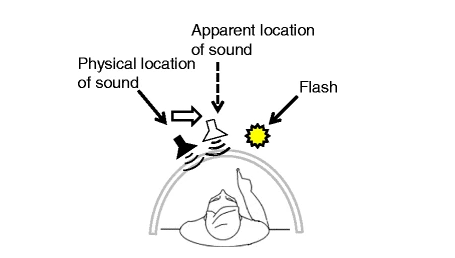
\includegraphics[width=0.55\textwidth]{04_antecedentes/figures/ventrilocuo.png}
    \caption{
        Ventriloquia espacial: la ubicación aparente de un sonido objetivo auditivo puede ser desplazada por la percepción de un estímulo visual (un destello).
    }
    \label{fig:patterns/ventrilocuo}
\end{figure}

% =============================================================================
% SECCIÓN 4: MODELOS BIOLÓGICAMENTE INSPIRADOS
% =============================================================================

\section{Modelos biológicamente inspirados}
\label{sec:modelos_biologicos}

La búsqueda de modelos computacionales que capturen los mecanismos neuronales de la cognición ha dado lugar a diversas aproximaciones, que varían en su nivel de abstracción y realismo biológico. En esta sección, vamos a revisar los principios fundamentales que guían el desarrollo de modelos biológicamente inspirados, con especial énfasis en aquellos que buscan implementar funciones computacionales mediante dinámicas neurológicamente plausibles.

\subsection{El paradigma de la ingeniería neuronal}
\label{subsec:ingenieria_neuronal}

El libro seminal \textit{Neural Engineering: Computation, Representation, and Dynamics in Neurobiological Systems} de \citet{eliasmith2003neural}, establece un marco sistemático para construir modelos que conectan la representación neuronal con la computación. Este paradigma, conocido como \textbf{ingeniería neuronal}, propone tres principios fundamentales:

\textbf{Principio 1: Representación.} Establece que las poblaciones de neuronas representan información mediante patrones de actividad distribuidos. Formalmente, si $\mathbf{x}$ es una variable que el sistema nervioso necesita representar, cada neurona $i$ en una población contribuye con una actividad:

\begin{equation}
a_i = G_i[\alpha_i \mathbf{e}_i \cdot \mathbf{x} + J_i^{bias}]
\label{eq:neural_encoding}
\end{equation}

donde $G_i[\cdot]$ es la función de transferencia de la neurona (típicamente un modelo LIF), $\alpha_i$ es un factor de ganancia, $\mathbf{e}_i$ es el ``vector de codificación'' preferido de la neurona, y $J_i^{bias}$ es una corriente de fondo \citep{eliasmith2003neural}. Este principio puede extenderse para representar no solo valores puntuales sino distribuciones de probabilidad completas.

\textbf{Principio 2: Transformación.} Especifica cómo las conexiones sinápticas entre poblaciones neuronales pueden implementar transformaciones matemáticas de las variables representadas. Dado que queremos computar una función, los pesos sinápticos óptimos pueden derivarse mediante métodos de optimización \citep{eliasmith2003neural}.

\textbf{Principio 3: Dinámica.} Describe cómo las propiedades temporales de las redes recurrentes permiten implementar sistemas dinámicos. La dinámica de una representación neuronal puede describirse mediante:

\begin{equation}
\frac{d\mathbf{x}}{dt} = f(\mathbf{x}, \mathbf{u})
\label{eq:neural_dynamics}
\end{equation}

donde $\mathbf{u}$ representa entradas externas y $f$ es la función que controla la evolución del sistema \citep{eliasmith2003neural}. Este principio es particularmente relevante cuando las dinámicas temporales, como transitorios y oscilaciones, no son meros epifenómenos sino que cumplen roles funcionales específicos en el procesamiento de información.

Estos principios proporcionan una metodología rigurosa para pasar de especificaciones funcionales a implementaciones neuronales. Sin embargo, enfoques más recientes han demostrado que es posible invertir esta lógica: partir de restricciones biológicas conocidas sobre la arquitectura de circuitos corticales, como la separación de poblaciones excitatorias e inhibitorias, funciones de transferencia supralineales, y ruido de proceso, y optimizar los parámetros para lograr una función computacional deseada, permitiendo que las dinámicas específicas emerjan como consecuencia de la optimización \citep{echeveste2020cortical}.

Independientemente del enfoque adoptado, una decisión fundamental es el nivel de detalle con que se modela la actividad neuronal. Los principios presentados pueden implementarse tanto con modelos de tasa como con modelos que capturan explícitamente los potenciales de acción individuales, cada uno con sus propias ventajas y limitaciones.

\subsection{Ruido y variabilidad neuronal}
\label{subsec:ruido_neuronal}

Una característica ubicua de la actividad neuronal es su \textbf{variabilidad}. Incluso bajo estimulación constante, las neuronas muestran fluctuaciones considerables en sus tiempos de disparo de trial a trial. Esta variabilidad, lejos de ser simplemente ``ruido'' que debe ignorarse, puede tener importantes funciones computacionales \citep{gerstner2002spiking}.

Las fuentes de variabilidad neuronal incluyen:

\begin{itemize}
    \item \textbf{Ruido de canal}: fluctuaciones estocásticas en la apertura y cierre de canales iónicos
    \item \textbf{Ruido sináptico}: variabilidad en la liberación de vesículas y en la respuesta postsináptica
    \item \textbf{Ruido de red}: actividad de fondo de otras neuronas en el circuito
\end{itemize}

En modelos computacionales, el ruido se incorpora típicamente como un término estocástico aditivo en las ecuaciones dinámicas. Un aspecto crítico es si este ruido es dependiente o independiente del estímulo. Como veremos en la Sección~\ref{sec:modelo_echeveste}, el modelo de Echeveste et al. incorpora específicamente \textbf{ruido de proceso independiente del estímulo}, una restricción biológica que resulta fundamental para las propiedades emergentes del circuito.

Crucialmente, la variabilidad neuronal puede tener un rol funcional en la inferencia probabilística. La hipótesis del \textbf{muestreo neuronal} propone que el cerebro representa distribuciones de probabilidad mediante muestras estocásticas de la actividad neuronal \citep{echeveste2020cortical}. En este marco, la variabilidad trial-a-trial no es ruido a eliminar sino una característica funcional que permite explorar el espacio de posibles interpretaciones de los estímulos sensoriales.

\subsection{Redes excitatorias-inhibitorias}
\label{subsec:redes_ei}

Partiendo de las bases del ya mencionado principio de Dale, al modelar los circuitos corticales con poblaciones separadas de neuronas excitatorias (E) e inhibitorias (I) también nos permite estudiar dinámicas que emergen de su interacción. En el régimen de \textbf{balance excitación-inhibición}, las corrientes excitatorias e inhibitorias a cada neurona se cancelan aproximadamente en promedio, manteniendo el potencial de membrana medio por debajo del umbral de disparo. En este régimen, los potenciales de acción ocurren solo cuando fluctuaciones en la entrada son suficientemente fuertes para alcanzar el umbral, generando patrones de disparo irregulares con alta variabilidad \citep{dayan2005theoretical}.

El \textbf{estado balanceado} tiene propiedades computacionalmente interesantes: genera actividad irregular similar a la observada en corteza, permite respuestas rápidas a cambios en la entrada, y puede implementar dinámicas de muestreo para inferencia probabilística \citep{echeveste2020cortical}. Estas propiedades hacen que las redes E-I balanceadas sean un punto fuerte para modelos de procesamiento cortical.

\medskip

Los principios y restricciones biológicas presentados en esta sección definen el espacio de arquitecturas biológicamente plausibles. Sin embargo, especificar la arquitectura no determina los valores de los parámetros (pesos sinápticos, constantes de tiempo) que permiten a la red realizar una función computacional específica. Para encontrar estos parámetros, los enfoques modernos recurren a técnicas desarrolladas en el campo del aprendizaje automático, que revisaremos en la siguiente sección.

% =============================================================================
% SECCIÓN 5: MACHINE LEARNING APLICADO A LA NEUROCIENCIA
% =============================================================================

\section{Machine learning aplicado a la neurociencia}
\label{sec:machine_learning}

El aprendizaje automático (\textit{machine learning}) es el campo de estudio en el cual un programa de computadora aprende de una experiencia $E$ respecto a una clase de tareas $T$ y una medida de rendimiento $P$, si su rendimiento en las tareas de $T$, medida por $P$, mejora con la experiencia $E$ \citep{mitchell1997machine}. Esta disciplina y la neurociencia han mantenido una relación simbiótica desde sus orígenes: por un lado, el cerebro ha inspirado muchos de los algoritmos de aprendizaje más exitosos, y por otro, las técnicas de machine learning proporcionan herramientas poderosas para analizar datos neuronales y desarrollar modelos computacionales del cerebro \citep{heaton2018ian}. En esta sección, revisamos los conceptos fundamentales de machine learning relevantes para el modelado neurocientífico.

\subsection{Paradigmas de aprendizaje}
\label{subsec:paradigmas_aprendizaje}

El aprendizaje automático puede clasificarse en tres paradigmas principales según la naturaleza de la señal de entrenamiento disponible \citep{bishop2006pattern, murphy2012machine}.

El \textbf{aprendizaje supervisado} opera cuando se dispone de pares entrada-salida etiquetados $\{(\mathbf{x}_i, \mathbf{y}_i)\}_{i=1}^N$. El objetivo es aprender una función $f$ que mapee entradas a salidas correctamente, típicamente minimizando una función de pérdida:

\begin{equation}
\mathcal{L} = \sum_{i=1}^N L(f(\mathbf{x}_i; \boldsymbol{\theta}), \mathbf{y}_i)
\label{eq:supervised_loss}
\end{equation}

donde $\boldsymbol{\theta}$ son los parámetros del modelo y $L$ mide la discrepancia entre predicciones y etiquetas. En el contexto neurocientífico, el aprendizaje supervisado se utiliza para entrenar redes neuronales que reproduzcan aspectos específicos de la actividad cortical o del comportamiento.

El \textbf{aprendizaje no supervisado} busca descubrir estructura en datos sin etiquetas. Esto incluye tareas como el agrupamiento (\textit{clustering}), la reducción de dimensionalidad, y la estimación de densidad. El \acrfull{PCA} es un ejemplo clásico, utilizado frecuentemente para identificar patrones de covariación en poblaciones neuronales \citep{bishop2006pattern}.

El \textbf{aprendizaje por refuerzo} considera un agente que interactúa con un ambiente y recibe señales de recompensa, aprendiendo una política que maximice la recompensa acumulada a largo plazo \citep{bishop2006pattern}.

En el contexto del presente trabajo, el paradigma relevante es el aprendizaje supervisado, aunque con una particularidad importante: en lugar de entrenar una red para producir una salida puntual correcta, el objetivo es que la \textit{distribución} de respuestas de la red coincida con una distribución objetivo. Esto requiere definir funciones de pérdida que comparen estadísticas de las respuestas (como media y covarianza) con los valores objetivo derivados de un modelo generativo. Este enfoque, desarrollado por \cite{echeveste2020cortical}, será detallado en la Sección~\ref{sec:modelo_echeveste}.

\subsection{Redes neuronales artificiales}
\label{subsec:redes_artificiales}

Las \acrfull{ANN} son modelos computacionales inspirados en la estructura del cerebro, compuestos por unidades de procesamiento interconectadas organizadas en capas \citep{heaton2018ian}. Aunque difieren significativamente de las redes biológicas en muchos detalles, capturan principios importantes de procesamiento distribuido y aprendizaje mediante ajuste de conexiones.

El \acrfull{MLP} es la arquitectura más básica. Cada capa $l$ computa:

\begin{equation}
\mathbf{h}^{(l)} = \sigma(\mathbf{W}^{(l)}\mathbf{h}^{(l-1)} + \mathbf{b}^{(l)})
\label{eq:mlp_layer}
\end{equation}

donde $\mathbf{h}^{(l)}$ son las activaciones de la capa $l$, $\mathbf{W}^{(l)}$ es la matriz de pesos, $\mathbf{b}^{(l)}$ es el vector de sesgos, y $\sigma(\cdot)$ es una función de activación no lineal \citep{heaton2018ian}.

Un avance fundamental para el entrenamiento de estas redes fue el algoritmo de \textbf{retropropagación} (\textit{backpropagation}), popularizado por \citet{rumelhart1986learning}. Este algoritmo permite ajustar los pesos de todas las capas simultáneamente, propagando los gradientes del error desde la salida hacia la entrada mediante la regla de la cadena:

\begin{equation}
\frac{\partial \mathcal{L}}{\partial \mathbf{W}^{(l)}} = \frac{\partial \mathcal{L}}{\partial \mathbf{h}^{(l)}} \frac{\partial \mathbf{h}^{(l)}}{\partial \mathbf{W}^{(l)}}
\label{eq:backprop}
\end{equation}

La importancia de este algoritmo para el campo fue reconocida con el Premio Turing 2018, otorgado a Geoffrey Hinton, Yoshua Bengio y Yann LeCun por sus contribuciones al aprendizaje profundo, y más recientemente con el Premio Nobel de Física 2024 a Hinton y John Hopfield por los fundamentos del aprendizaje automático con redes neuronales artificiales \citep{hinton2024nobel}. En el contexto del presente trabajo, la retropropagación a través del tiempo (\textit{backpropagation through time}) constituye la base para optimizar los parámetros de redes recurrentes como la de \citet{echeveste2020cortical}, donde se combina con optimizadores modernos como ADAM y L-BFGS-B.

\subsection{Arquitecturas profundas y convolucionales}
\label{subsec:arquitecturas_profundas}

El \textbf{aprendizaje profundo} (\textit{deep learning}) se refiere al entrenamiento de redes neuronales con múltiples capas ocultas. La profundidad permite aprender representaciones jerárquicas donde las capas inferiores extraen características simples y las superiores combinan estas en representaciones más abstractas \citep{heaton2018ian}.

Las \acrfull{CNN} son particularmente relevantes para el procesamiento visual. Inspiradas en la organización jerárquica del sistema visual, las CNNs aplican filtros convolucionales que son equivariantes a traslaciones:

\begin{equation}
(h * w)[i,j] = \sum_m \sum_n h[m,n] \cdot w[i-m, j-n]
\label{eq:convolution}
\end{equation}

Notablemente, CNNs entrenadas para clasificación de imágenes desarrollan representaciones en sus capas ocultas que correlacionan fuertemente con la actividad neuronal a lo largo de la jerarquía visual, desde V1 hasta corteza inferotemporal \citep{yamins2014performance}.

\begin{figure}[H]
    \centering
    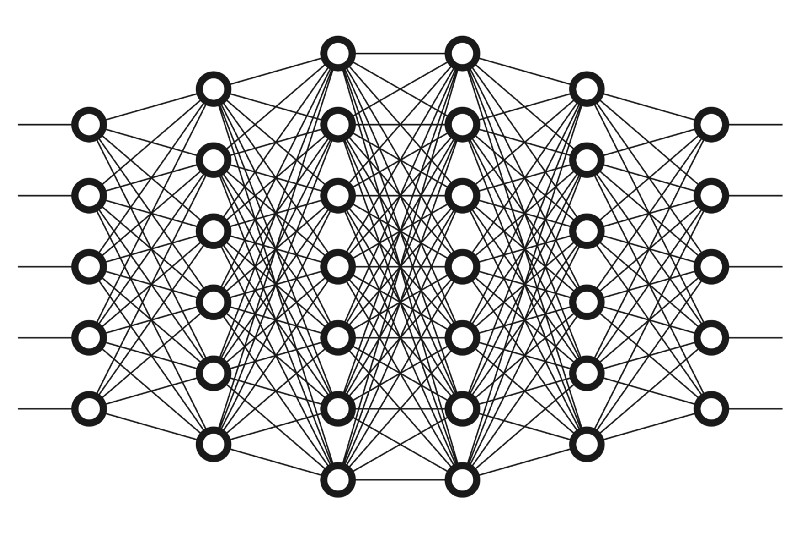
\includegraphics[width=0.55\textwidth]{04_antecedentes/figures/deep-learning.jpg}
    \caption{
        Representación de una red neuronal profunda. Se ilustra la organización en múltiples capas ocultas que permite la extracción jerárquica de características, desde rasgos simples a representaciones abstractas.
    }
    \label{fig:patterns/deep-learning}
\end{figure}

\subsection{Redes recurrentes}
\label{subsec:redes_tipo_recurrentes}

Como se discutió en la Sección~\ref{subsec:redes_recurrentes}, los circuitos corticales se caracterizan por conexiones recurrentes abundantes que permiten generar dinámicas temporales complejas. Las \acrfull{RNN} constituyen el análogo computacional de estos circuitos biológicos, extendiendo las redes feedforward al incluir conexiones que forman ciclos, permitiendo que la actividad pasada influya en el procesamiento presente \citep{heaton2018ian}. La dinámica de una RNN simple está dada por:

\begin{equation}
\mathbf{h}_t = \sigma(\mathbf{W}_{hh}\mathbf{h}_{t-1} + \mathbf{W}_{xh}\mathbf{x}_t + \mathbf{b})
\label{eq:rnn}
\end{equation}

donde $\mathbf{h}_t$ es el estado oculto en el tiempo $t$ y $\mathbf{x}_t$ es la entrada.

Arquitecturas como \acrfull{LSTM} y \acrfull{GRU} incorporan mecanismos de compuerta que permiten mantener información relevante a lo largo de secuencias largas \citep{heaton2018ian}.

En el contexto de este trabajo, las RNNs con restricciones biológicas dadas por poblaciones E-I separadas, funciones de activación plausibles y ruido de proceso, proporcionan un marco para estudiar cómo las dinámicas corticales pueden implementar funciones computacionales como la inferencia probabilística.

\begin{figure}[H]
\begin{minipage}{0.45\linewidth}
    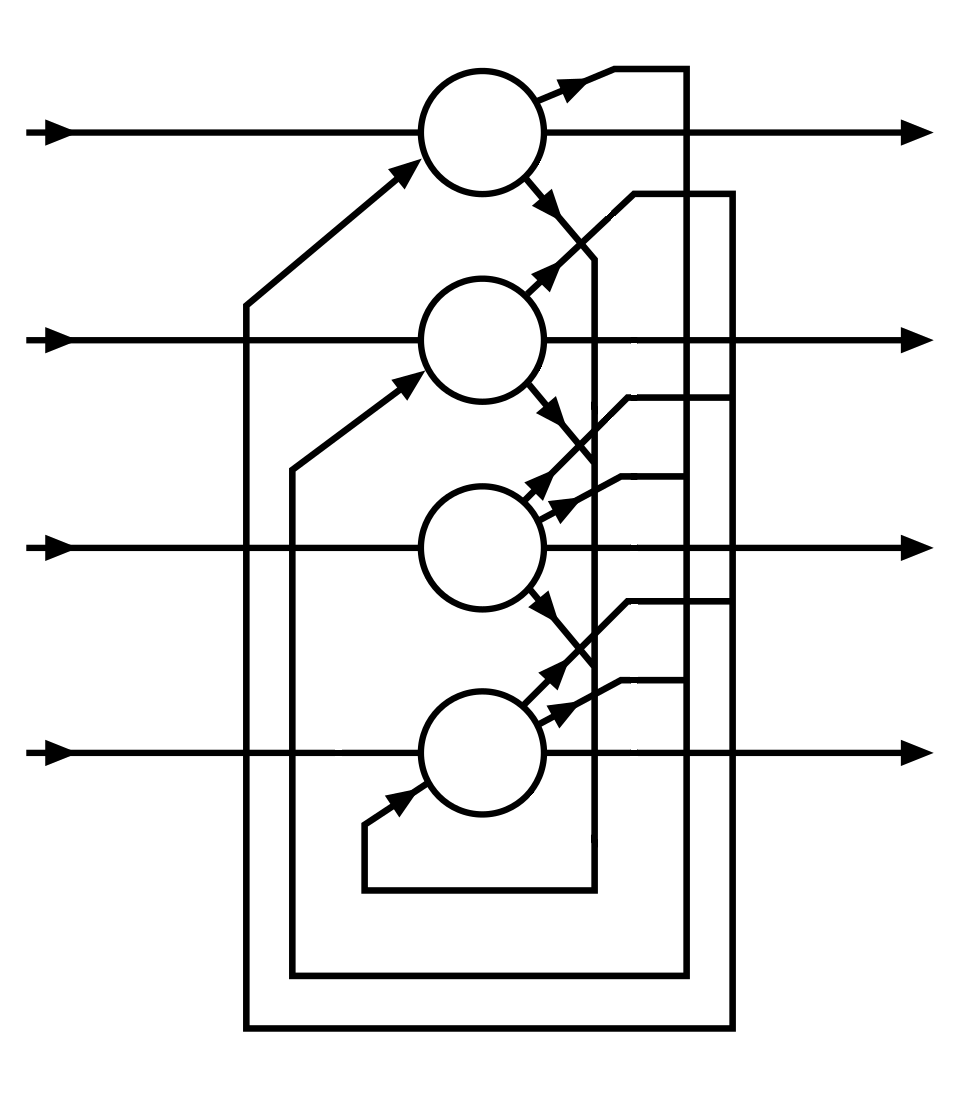
\includegraphics[width=\linewidth]{04_antecedentes/figures/rnn.png}
\end{minipage}\hfill
\begin{minipage}{0.5\linewidth}
    \caption{
        Red neuronal recurrente totalmente conectada con 4 neuronas.
    }
    \label{fig:rnn}
\end{minipage}
\end{figure}

\subsection{Estadística bayesiana y aprendizaje}
\label{subsec:bayesiana_aprendizaje}

El marco \textbf{bayesiano} proporciona una interpretación probabilística del aprendizaje donde los parámetros del modelo son tratados como variables aleatorias con distribuciones de probabilidad \citep{bishop2006pattern}. Dada una verosimilitud $P(\mathcal{D}|\boldsymbol{\theta})$ para los datos y un prior $P(\boldsymbol{\theta})$ sobre los parámetros, el teorema de Bayes proporciona la distribución posterior:

\begin{equation}
P(\boldsymbol{\theta}|\mathcal{D}) = \frac{P(\mathcal{D}|\boldsymbol{\theta})P(\boldsymbol{\theta})}{P(\mathcal{D})}
\label{eq:bayes_learning}
\end{equation}

Esta perspectiva es particularmente relevante para la neurociencia computacional. 
Diversos autores han propuesto que el cerebro opera según principios bayesianos, 
manteniendo y actualizando distribuciones de probabilidad sobre estados del mundo 
\citep{dayan2005theoretical, eliasmith2003neural}.

La \textbf{inferencia aproximada} es necesaria cuando la distribución posterior 
no puede calcularse analíticamente. Métodos como Markov Chain Monte Carlo (MCMC) 
y la inferencia variacional proporcionan aproximaciones tractables 
\citep{heaton2018ian}. Como veremos, estos métodos tienen análogos propuestos 
en dinámicas neuronales.

\subsection{Redes neuronales para inferencia probabilística}
\label{subsec:redes_inferencia}

Un aspecto fundamental para este trabajo es comprender cómo redes neuronales pueden implementar inferencia probabilística. La hipótesis del \textbf{muestreo neuronal} propone que las fluctuaciones en la actividad neuronal representan muestras de 
distribuciones de probabilidad, de modo que la actividad promediada en el tiempo corresponde a esperanzas bajo distribuciones posteriores \citep{echeveste2020cortical}.

Formalmente, si un circuito neuronal implementa muestreo de una distribución $P(\mathbf{x}|\mathbf{s})$ donde $\mathbf{s}$ es un estímulo, entonces la actividad instantánea $\mathbf{x}(t)$ representa una muestra, y:

\begin{equation}
\langle \mathbf{x}(t) \rangle_t \approx \mathbb{E}_{P(\mathbf{x}|\mathbf{s})}[\mathbf{x}]
\label{eq:neural_sampling}
\end{equation}

Esta perspectiva tiene implicaciones profundas para interpretar la variabilidad neuronal, sugiriendo que no es simplemente ruido sino que codifica incertidumbre sobre el estado del mundo.

Recientemente, se ha demostrado que redes neuronales recurrentes con restricciones biológicas pueden ser entrenadas para implementar muestreo de distribuciones posteriores complejas, mostrando simultáneamente propiedades dinámicas similares a las observadas en corteza \citep{echeveste2020cortical}. Este resultado establece un puente crucial entre la función computacional (inferencia probabilística) y los mecanismos neuronales (dinámicas corticales), y constituye un antecedente directo del presente trabajo.

% =============================================================================
% SECCIÓN 6: MODELOS Y HERRAMIENTAS PARA EL PRESENTE TRABAJO
% =============================================================================

\section{Antecedentes directos}
\label{subsec:antecedentes_directos}

Los fundamentos presentados en este capítulo, desde los mecanismos biológicos de la señalización neuronal hasta las técnicas de aprendizaje automático para optimizar redes recurrentes, proporcionan el marco conceptual y metodológico para abordar el problema central de este trabajo. En esta sección final presentamos brevemente los antecedentes específicos que, desarrollados en detalle en sus respectivos capítulos, constituyen la motivación y el punto de partida de nuestra contribución.

Entre los desarrollos que buscan implementar los principios de inferencia probabilística en arquitecturas biológicamente plausibles, dos modelos resultan particularmente relevantes para este trabajo.

El modelo de \citet{cuppini2017biologically} aborda la integración audiovisual y el efecto ventrílocuo mediante una arquitectura de tres capas que reproduce exitosamente fenómenos experimentales como el juicio de unidad. Sin embargo, al utilizar modelos de tasa deterministas, no captura las dinámicas corticales realistas observadas experimentalmente. 

En contraste, el modelo de \citet{echeveste2020cortical} demuestra que redes neuronales con restricciones biológicas pueden implementar inferencia probabilística mediante muestreo, exhibiendo propiedades emergentes como oscilaciones gamma y transitorios inhibitorios. Sin embargo, está limitado al procesamiento unimodal. Los detalles de ambos modelos están desarrollados en el Capítulo~\ref{chapter:modelos_estudiados}.

Más allá de sus diferencias conceptuales, ambos modelos comparten una limitación práctica ya que han sido implementados de manera independiente, en distintos lenguajes y con estructuras incompatibles, dificultando su comparación o integración. Para abordar este tipo de fragmentación en el campo, \citet{paredes2025scikit} desarrollaron Scikit-NeuroMSI, un framework de código abierto en Python que proporciona infraestructura común para la implementación, comparación y validación de modelos de integración multisensorial. Presentando todas sus características técnicas en el Capítulo~\ref{chapter:scikit_neuromsi}.

% \subsection{Objetivo y contribución del presente trabajo}
% \label{subsec:objetivo_contribucion}

% La revisión presentada revela una brecha significativa: los modelos de integración multisensorial como el de Cuppini capturan la arquitectura funcional pero carecen de dinámicas corticales realistas, mientras que modelos como el de Echeveste exhiben dinámicas biológicamente plausibles pero están limitados al procesamiento unimodal. Además, cada modelo ha sido implementado independientemente, dificultando cualquier intento de integración.

% La visión a largo plazo que motiva este trabajo es el desarrollo de modelos que combinen la arquitectura multimodal del modelo de Cuppini con las dinámicas corticales del modelo de Echeveste. Sin embargo, alcanzar esta visión requiere primero sentar bases técnicas sólidas. El presente trabajo representa el primer paso en esta dirección mediante la implementación del modelo de Echeveste dentro del framework Scikit-NeuroMSI.

% Esta implementación incluye la arquitectura de red con poblaciones excitatorias e inhibitorias, el modelo generativo GSM con cálculo de momentos objetivo, y el procedimiento de entrenamiento para muestreo. La validación verificará que el modelo reproduce las propiedades reportadas originalmente: convergencia de momentos, variabilidad modulada por contraste, y presencia de dinámicas temporales características.

% Junto con el modelo, el trabajo desarrolla bases para las herramientas de análisis necesarias para estudiar modelos con dinámicas temporales relevantes. Estas herramientas permitirán visualizar la evolución de los potenciales de membrana, calcular espectros de potencia para identificar oscilaciones, y comparar estadísticas de las respuestas con los valores objetivo. Aunque desarrolladas para el modelo de Echeveste, estas herramientas pueden ser modificadas y quedarán disponibles para cualquier modelo futuro que requiera análisis de dinámicas temporales.

% Es importante delimitar lo que este trabajo no aborda: la fusión con el modelo de Cuppini y la implementación de inferencia causal multisensorial quedan como direcciones futuras. El presente trabajo se enfoca en establecer las bases técnicas que harán posibles estas extensiones, reconociendo que una implementación correcta del modelo de Echeveste es condición necesaria para cualquier desarrollo posterior hacia el procesamiento multisensorial con dinámicas corticales realistas. \cleardoublepage 
\chapter{Modelos Estudiados}
\label{chapter:modelos_estudiados}

Este capítulo presenta en detalle los dos modelos computacionales que constituyen los pilares conceptuales del presente trabajo. El modelo de \citeauthor{cuppini2017biologically} aborda la integración audiovisual y la inferencia causal mediante una arquitectura neuronal biológicamente inspirada, representando el objetivo a largo plazo hacia el cual apuntan las extensiones futuras de este trabajo. Y en la otra mano el modelo de \citeauthor{echeveste2020cortical} demuestra cómo circuitos corticales con restricciones biológicas pueden implementar inferencia probabilística mediante muestreo, exhibiendo dinámicas realistas como oscilaciones gamma y transitorios inhibitorios. Este segundo modelo constituye el objeto central de implementación del presente trabajo.

% =============================================================================
% SECCIÓN 1: EL MODELO DE CUPPINI
% =============================================================================

\section{El modelo de Cuppini para integración audiovisual e inferencia causal}
\label{sec:modelo_cuppini}

El problema de la inferencia causal multisensorial descripto en la Sección~\ref{subsec:inferencia_causal} ha motivado el desarrollo de diversos modelos computacionales. Entre ellos, el modelo desarrollado por \citet{cuppini2017biologically} representa un avance significativo al abordar específicamente la integración audiovisual y el efecto ventrílocuo mediante una arquitectura neuronal biológicamente inspirada.

\subsection{Arquitectura del modelo}
\label{subsec:cuppini_arquitectura}

El modelo se estructura en tres capas jerárquicas interconectadas, cada una compuesta por neuronas organizadas topográficamente según la posición espacial de su campo receptivo.

La \textbf{capa auditiva} procesa información sobre la localización espacial de estímulos sonoros. Cada unidad en esta capa responde preferentemente a sonidos provenientes de una posición específica del espacio, aunque con campos receptivos relativamente amplios que reflejan la menor precisión espacial de la audición comparada con la visión.

La \textbf{capa visual} procesa información sobre la localización de estímulos visuales. Las unidades en esta capa tienen campos receptivos más estrechos que sus contrapartes auditivas, capturando la mayor resolución espacial del sistema visual.

La \textbf{capa multisensorial} (o de inferencia causal) recibe proyecciones feedforward de ambas capas unisensoriales y computa la integración de señales y la decisión sobre la estructura causal subyacente.

Las capas se interconectan mediante tres tipos de sinapsis: conexiones \textit{laterales intra-área} organizadas en un perfil de ``sombrero mexicano'' que implementa competencia local, conexiones \textit{cross-modales} excitatorias recíprocas entre las capas auditiva y visual, y proyecciones \textit{feedforward} hacia la capa multisensorial.

\begin{figure}[!ht]
    \centering
    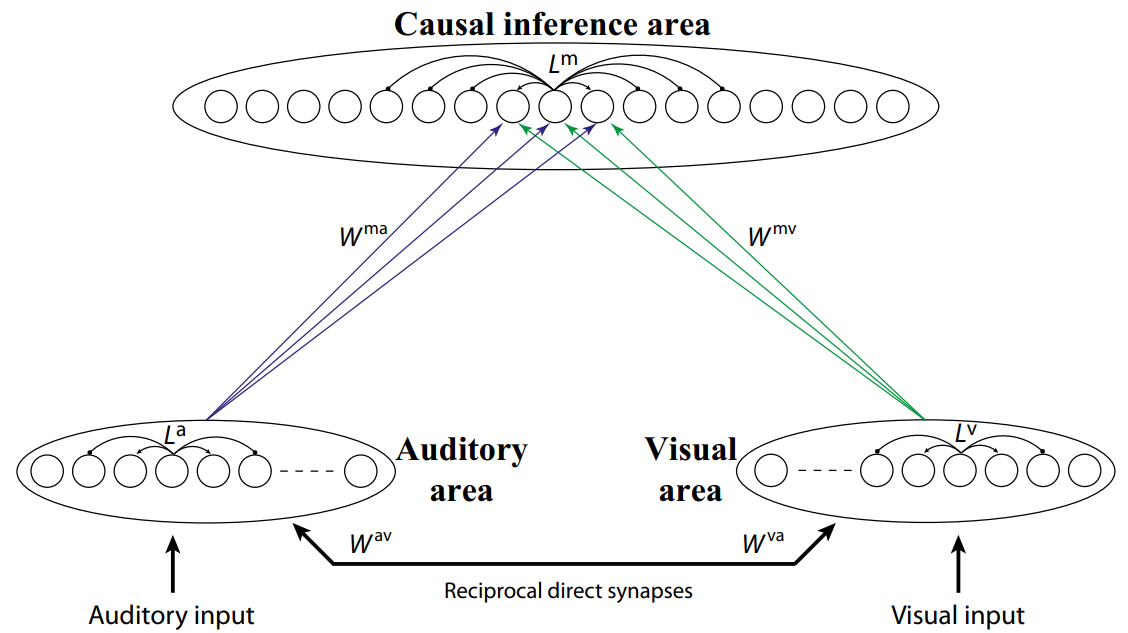
\includegraphics[width=0.95\textwidth]{04_antecedentes/figures/cuppini.png}
    \caption{
        Estructura de la red de \citeauthor{cuppini2017biologically}. Las regiones visual y auditiva procesan los estímulos sensoriales externos. Estas regiones están interconectadas mediante sinapsis excitatorias directas y envían proyecciones feedforward de largo alcance dirigidas al área de inferencia causal.
    }
    \label{fig:patterns/template_method}
\end{figure}

\subsection{Mecanismos de integración e inferencia}
\label{subsec:cuppini_mecanismos}

El modelo implementa dos mecanismos computacionales distintos pero interrelacionados:

El primer mecanismo, mediado por las \textbf{sinapsis cross-modales} entre las capas unisensoriales, produce la integración clásica multisensorial. Cuando estímulos visual y auditivo se presentan en posiciones espaciales cercanas, las conexiones cross-modales excitatorias refuerzan mutuamente las actividades en ambas regiones, atrayendo las representaciones espaciales hacia una posición común. Este mecanismo da lugar al efecto ventrílocuo: el sesgo de la localización auditiva percibida hacia la posición del estímulo visual.

El segundo mecanismo, mediado por la \textbf{capa multisensorial}, computa la inferencia causal propiamente dicha. La actividad en esta capa integra información de ambas modalidades y determina si los estímulos se perciben como provenientes de una causa común o de fuentes independientes. La presencia de uno o dos picos de actividad por encima de un umbral de detección indica, respectivamente, la inferencia de una causa única o de causas separadas.

\subsection{Capacidades y limitaciones}
\label{subsec:cuppini_limitaciones}

El modelo reproduce exitosamente varios fenómenos experimentales: \textbf{el efecto ventrílocuo} emerge naturalmente de la dinámica, con magnitud dependiente de la confiabilidad relativa de las señales; \textbf{el juicio de unidad} exhibe el patrón correcto donde la probabilidad de percibir una causa común disminuye con la disparidad espacial; y el \textbf{sesgo auditivo} es modulado por la decisión causal, siendo mayor cuando se infiere una causa común \citep{cuppini2017biologically}.

Sin embargo, el modelo presenta limitaciones significativas desde la perspectiva de la neurociencia computacional moderna. Al utilizar modelos de tasa deterministas, no captura fenómenos característicos de la actividad cortical real como la variabilidad \textit{trial-a-trial}, es decir, las fluctuaciones en las respuestas neuronales entre presentaciones repetidas de un mismo estímulo; las oscilaciones gamma observadas durante la integración multisensorial; los transitorios inhibitorios, donde la inhibición domina brevemente al inicio de la estimulación antes de estabilizarse; ni la naturaleza estocástica de la inferencia perceptual.

Estas limitaciones motivaron inicialmente el presente trabajo, con el objetivo a largo plazo de desarrollar modelos de integración multisensorial que exhiban dinámicas corticales biológicamente plausibles. El modelo de \citeauthor{echeveste2020cortical}, descrito en la siguiente sección, demuestra que tales dinámicas pueden emerger de redes neuronales optimizadas para inferencia probabilística.

% =============================================================================
% SECCIÓN 2: EL MODELO DE ECHEVESTE (EXPANDIDO)
% =============================================================================

\section{El modelo de Echeveste para inferencia probabilística con dinámicas corticales}
\label{sec:modelo_echeveste}

En contraste con el modelo anterior, el trabajo de \citet{echeveste2020cortical} aborda el problema desde la dirección opuesta: partiendo de restricciones biológicas sobre la dinámica de circuitos corticales, demuestran que redes neuronales recurrentes pueden ser optimizadas para implementar inferencia probabilística basada en muestreo. Este modelo constituye un antecedente fundamental para el presente trabajo, por lo que a continuación se presenta una descripción detallada de sus componentes.

\subsection{Marco teórico: muestreo como inferencia}
\label{subsec:echeveste_marco}

La percepción puede entenderse como inferencia bayesiana sobre las causas latentes de las observaciones sensoriales. Dado un estímulo sensorial $\mathbf{x}$, el cerebro busca inferir las variables latentes $\mathbf{y}$ que lo generaron, caracterizadas por la distribución posterior enunciada en la Ecuación \ref{eq:bayes_perception}.

La hipótesis del \textbf{muestreo neuronal} propone que, en lugar de representar esta distribución analíticamente, el cerebro la representa mediante muestras temporales. La actividad neuronal fluctuante proporciona muestras de la posterior, de modo que la distribución empírica de actividades a lo largo del tiempo aproxima $P(\mathbf{y}|\mathbf{x})$ \citep{echeveste2020cortical}. Formalmente, si $\mathbf{y}(t)$ representa la actividad neuronal instantánea:


\begin{equation}
\langle \mathbf{y}(t) \rangle_t \approx \mathbb{E}_{P(\mathbf{y}|\mathbf{x})}[\mathbf{y}]
\label{eq:neural_sampling_mean}
\end{equation}

El lado izquierdo de esta ecuación denota el promedio temporal de la actividad neuronal, es decir, la media de las respuestas observadas a lo largo de una ventana de tiempo. El lado derecho representa el valor esperado de las variables latentes bajo la distribución posterior. La ecuación expresa que, si la red neuronal efectivamente muestrea de la posterior, entonces acumular y promediar estas muestras a lo largo del tiempo converge hacia la media de dicha distribución, análogamente a cómo los métodos de Monte Carlo aproximan valores esperados mediante promedios empíricos de muestras \citep{gerstner2002spiking}. Del mismo modo, la variabilidad y las correlaciones en las respuestas neuronales codifican la estructura de incertidumbre de la posterior.


Esta perspectiva transforma la variabilidad neuronal de un fenómeno a ignorar en una característica funcional que codifica incertidumbre perceptual.

\subsection{Arquitectura de red}
\label{subsec:echeveste_arquitectura}

La red modela una \textbf{hipercolumna} de la corteza visual primaria (V1): una unidad funcional que contiene neuronas sensibles a todas las orientaciones posibles de bordes visuales en una misma ubicación del campo visual. Las neuronas se organizan conceptualmente en un \textbf{anillo}, donde la posición de cada una corresponde a su orientación preferida, distribuida uniformemente entre $-90^\circ$ y $90^\circ$ (ver Figura~\ref{fig:arquieche}).

La red contiene dos poblaciones: \textbf{excitatorias} (E) e \textbf{inhibitorias} (I), organizadas en pares E-I que comparten la misma orientación preferida. Cada neurona excitatoria representa una variable latente del modelo generativo \acrshort{GSM} es decir, la intensidad de una característica visual orientada, mientras que las neuronas inhibitorias actúan como unidades auxiliares que estabilizan la dinámica del circuito.

La conectividad entre neuronas depende de la \textbf{diferencia de orientación} entre ellas: neuronas con orientaciones similares tienen conexiones más fuertes que neuronas con orientaciones diferentes. Esta estructura ``circulante'' refleja la organización columnar observada en V1 y reduce drásticamente el número de parámetros libres de $N^2$ a solo 8 parámetros que definen el perfil de conectividad.

\begin{figure}[!ht]
    \centering
    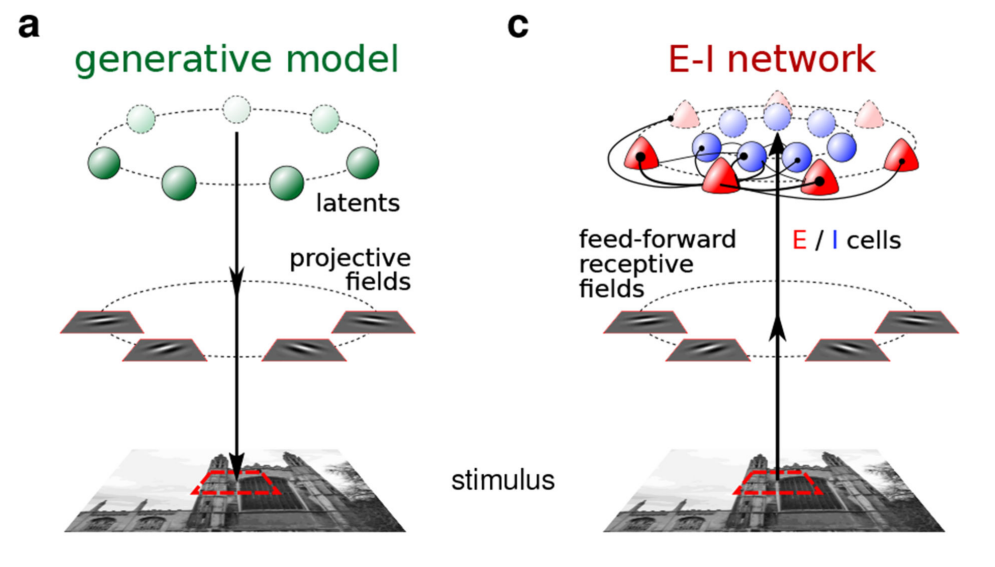
\includegraphics[width=0.90\textwidth]{04_antecedentes/figures/arquieche.png}
    \caption{
        % a, Esquema del GSM. Un parche de imagen se construye como una combinación lineal de un conjunto fijo de características localizadas y orientadas, similares a las de un filtro de Gabor.
        % b, proyección bidimensional de la distribución posterior sobre variables latentes dado un estímulo visual, calculada por el observador ideal bayesiano bajo el modelo generativo.
        El modelo generativo estadístico y el circuito neuronal correspondiente que implementa la inferencia probabilística basada en muestreo.
    }
    \label{fig:arquieche}
\end{figure}


\subsection{El modelo generativo (GSM)}
\label{subsec:echeveste_gsm}

Para especificar el problema computacional objetivo, los autores adoptan el \textbf{modelo de mezcla de escala gaussiana} (\acrfull{GSM}), un modelo generativo bien establecido que captura las estadísticas de parches de imágenes naturales \citep{echeveste2020cortical}. En este modelo, un parche de imagen $\mathbf{x} \in \mathbb{R}^{N_x}$ se genera como:

\begin{equation}
\mathbf{x} | \mathbf{y}, z \sim \mathcal{N}(z \mathbf{A} \mathbf{y}, \sigma_x^2 \mathbf{I})
\label{eq:gsm_likelihood}
\end{equation}

donde $\mathbf{y} \in \mathbb{R}^{N_y}$ son las variables latentes que representan intensidades de características visuales, $\mathbf{A} \in \mathbb{R}^{N_x \times N_y}$ es la matriz de \textit{campos proyectivos} (cuyas columnas son filtros tipo Gabor orientados, como se describió en la Sección~\ref{subsec:filtros_gabor}), $z \in \mathbb{R}$ es una variable de contraste global, y $\sigma_x^2$ es la varianza del ruido sensorial.

Las variables latentes siguen un prior gaussiano multivariado:

\begin{equation}
\mathbf{y} \sim \mathcal{N}(\mathbf{0}, \mathbf{C})
\label{eq:gsm_prior}
\end{equation}

donde $\mathbf{C}$ es la matriz de covarianza del prior, parametrizada como matriz circulante cuyos elementos varían suavemente en función de la diferencia angular entre las orientaciones preferidas de los campos proyectivos correspondientes.

Para modelar inferencia en una hipercolumna de V1, los campos proyectivos (columnas de $\mathbf{A}$) se eligen como filtros de Gabor orientados que difieren únicamente en su orientación, distribuidos uniformemente entre $-90^\circ$ y $90^\circ$, formando así una topología de anillo.

\begin{equation}
\mathbf{x} = z \cdot \mathbf{A}\mathbf{y} + \boldsymbol{\epsilon}
\label{eq:gsm}
\end{equation}

donde $\mathbf{y}$ son variables latentes (intensidades de características visuales como filtros de Gabor), $\mathbf{A}$ es la matriz de campos proyectivos, $z$ es una variable de contraste global, y $\boldsymbol{\epsilon}$ es ruido sensorial.

\subsubsection{Distribución posterior del observador ideal}

Bajo el \acrshort{GSM}, la distribución posterior sobre las variables latentes dado un parche de imagen y un contraste conocido tiene forma gaussiana:

\begin{equation}
P_{\text{GSM}}(\mathbf{y}|\mathbf{x}, z) = \mathcal{N}(\mathbf{y}; \boldsymbol{\mu}_{\text{GSM}}, \boldsymbol{\Sigma}_{\text{GSM}})
\label{eq:gsm_posterior}
\end{equation}

con media y covarianza posteriores dadas por:

\begin{equation}
\boldsymbol{\mu}_{\text{GSM}} = \frac{z}{\sigma_x^2} \boldsymbol{\Sigma}_{\text{GSM}} \mathbf{A}^\top \mathbf{x}
\label{eq:gsm_posterior_mean}
\end{equation}

\begin{equation}
\boldsymbol{\Sigma}_{\text{GSM}} = \left( \mathbf{C}^{-1} + \frac{z^2}{\sigma_x^2} \mathbf{A}^\top \mathbf{A} \right)^{-1}
\label{eq:gsm_posterior_cov}
\end{equation}

Nótese que la covarianza posterior \eqref{eq:gsm_posterior_cov} decrece con $z^2$: a mayor contraste, menor incertidumbre en la estimación. Por su parte, la media posterior \eqref{eq:gsm_posterior_mean} depende del contraste de manera que para contrastes altos converge hacia el valor verdadero de las variables latentes, mientras que para contrastes bajos se acerca a la media del prior (cero). Estas propiedades, mayor precisión y mejores estimaciones con mayor contraste, son características que la red neuronal deberá reproducir.

En el modelo, el contraste $z$ se aproxima con su valor verdadero $z^*$, dado que es un único escalar cuya inferencia integra información de todos los píxeles:

\begin{equation}
P_{\text{GSM}}(\mathbf{y}|\mathbf{x}) \approx P_{\text{GSM}}(\mathbf{y}|\mathbf{x}, z^*)
\label{eq:gsm_marginal}
\end{equation}


\subsubsection{Transformación de variables latentes a potenciales de membrana}

Siguiendo trabajos previos, los potenciales de membrana $u_i$ se toman como una transformación débilmente no lineal de las activaciones de características visuales $y_i$:

\begin{equation}
u_i(y_i) = \left[ \alpha_{\text{nl}} y_i + \beta_{\text{nl}} \right]_+^{\gamma_{\text{nl}}}
\label{eq:latent_to_membrane}
\end{equation}

donde $[\cdot]_+$ denota la función de rectificación (threshold-linear), y $\alpha_{\text{nl}}$, $\beta_{\text{nl}}$, $\gamma_{\text{nl}}$ son respectivamente la escala, línea base y exponente de la transformación. Esta transformación permite que los potenciales de membrana representen las intensidades de características mientras respetan restricciones biológicas como la no-negatividad.

\subsection{Dinámica neuronal}
\label{subsec:echeveste_dinamica}

El modelo implementa una \textbf{red supralineal estabilizada} \acrfull{SSN}, una arquitectura que captura propiedades esenciales de los circuitos corticales. La red consiste en $N_E$ neuronas excitatorias y $N_I$ neuronas inhibitorias. La dinámica de cada neurona $i$ está controlada por:

\begin{equation}
\tau_i \frac{du_i}{dt} = -u_i(t) + h_i(t) + \sum_j W_{ij} r_j(t) + \eta_i(t)
\label{eq:ssn_dynamics}
\end{equation}

donde $u_i$ es el potencial de membrana, $h_i$ es la entrada feedforward dependiente del estímulo, $W_{ij}$ son los pesos sinápticos recurrentes, $r_j$ es la tasa de disparo de la neurona $j$, y $\eta_i(t)$ es ruido de proceso correlacionado temporalmente.

\subsubsection{Función de transferencia supralineal}

Las tasas de disparo se derivan de los potenciales de membrana mediante una función de transferencia supralineal:

\begin{equation}
r_i(t) = k \left[ u_i(t) \right]_+^n
\label{eq:firing_rate}
\end{equation}

donde $[\cdot]_+$ denota rectificación ($[x]_+ = \max(0, x)$), $k$ es un factor de escala, y $n > 1$ es el exponente supralineal (ambos parámetros fijos). Esta no linealidad es consistente con observaciones experimentales en neuronas corticales y resulta fundamental para las propiedades de estabilización del circuito. El término ``supralineal'' indica que la función es convexa para potenciales positivos, lo que produce respuestas que crecen más rápido que linealmente con la entrada.

\subsubsection{Parametrización de la conectividad (topología de anillo)}

Dado que la red debe exhibir la misma simetría circular que el GSM estructurado en anillo, la conectividad recurrente se parametriza de forma rotacionalmente simétrica. Las neuronas se organizan en pares E-I alrededor de un ``anillo'' según sus orientaciones preferidas, y la conectividad es una función gaussiana circular de la diferencia de orientación entre células.

Específicamente, cada cuadrante de la matriz de pesos ($E \rightarrow E$, $E \rightarrow I$, $I \rightarrow E$, $I \rightarrow I$) se define como:

\begin{equation}
W_{XY}(\theta_i, \theta_j) = a_{XY} \exp\left( \frac{\cos(2(\theta_i - \theta_j)) - 1}{d_{XY}^2} \right)
\label{eq:weight_parametrization}
\end{equation}

donde $X, Y \in \{E, I\}$, $\theta_i = \pi i / N_{E/I}$ es la orientación preferida de la $i$-ésima neurona E/I, $a_{XY}$ controla la amplitud de las conexiones, y $d_{XY}$ controla su ancho espacial.

Para respetar el \textbf{principio de Dale}, se imponen las siguientes restricciones sobre las amplitudes:
\begin{itemize}
    \item $a_{XE} > 0$ para $X \in \{E, I\}$ (conexiones desde neuronas excitatorias son positivas)
    \item $a_{XI} < 0$ para $X \in \{E, I\}$ (conexiones desde neuronas inhibitorias son negativas)
\end{itemize}

Esta parametrización circulante reduce drásticamente el número de parámetros libres: en lugar de optimizar todos los elementos de la matriz de pesos, para esta sección solo se optimizan 8 parámetros ($a_{XY}$ y $d_{XY}$ para cada cuadrante).

\subsubsection{Ruido de proceso}

El ruido de proceso $\eta_i(t)$ modela la variabilidad intrínseca y extrínseca de la actividad neuronal (entradas de otras áreas cerebrales, fluctuaciones de canal, etc.). Crucialmente, este ruido es \textbf{independiente del estímulo}, lo que implica que la red debe usar sus dinámicas recurrentes para moldear la variabilidad de manera apropiada para cada entrada.

El ruido es gaussiano con media cero y correlaciones espaciales y temporales:

\begin{equation}
\langle \eta_i(t) \rangle = 0, \quad \langle \eta_i(t) \eta_j(t+s)^\top \rangle = \Sigma_{ij}^\eta \exp(-|s|/\tau_\eta)
\label{eq:noise_correlation}
\end{equation}

% donde $\tau_\eta$ es la escala temporal del ruido y $\boldsymbol{\Sigma}^\eta$ es la matriz de covarianza espacial instantánea, también parametrizada de forma circulante con 4 parámetros adicionales ($\sigma_E$, $\sigma_I$, $\rho$, $d_\sigma$).

donde $\tau_\eta$ es la escala temporal del ruido y $\boldsymbol{\Sigma}^\eta$ es la matriz de covarianza espacial instantánea.

La covarianza espacial del ruido también se parametriza de forma circulante:

\begin{equation}
\Sigma_{EE/II}^\eta(\theta_i, \theta_j) = \sigma_{E/I}^2 \exp\left( \frac{\cos(2(\theta_i - \theta_j)) - 1}{d_\sigma^2} \right)
\label{eq:noise_cov_same}
\end{equation}

\begin{equation}
\Sigma_{EI}^\eta(\theta_i, \theta_j) = \rho \sigma_E \sigma_I \exp\left( \frac{\cos(2(\theta_i - \theta_j)) - 1}{d_\sigma^2} \right)
\label{eq:noise_cov_cross}
\end{equation}

donde $\sigma_E, \sigma_I > 0$ son las desviaciones estándar del ruido para poblaciones E e I, $\rho$ es el coeficiente de correlación entre ruido E e I, y $d_\sigma$ controla el ancho espacial de las correlaciones de ruido. Esto introduce 4 parámetros adicionales para el entrenamiento.

\subsubsection{Entrada feedforward}

La entrada dependiente del estímulo a cada neurona se obtiene aplicando un filtro lineal al estímulo seguido de una no linealidad estática:

\begin{equation}
h_i(t) = \left[ \alpha_h \left( \beta_h + \sum_j W_{ij}^{ff} x_j(t) \right) \right]_+^{\gamma_h}
\label{eq:feedforward_input}
\end{equation}

donde $\mathbf{x}(t)$ es el estímulo (parche de imagen), $\mathbf{W}^{ff}$ es la matriz de campos receptivos feedforward, y $\alpha_h$, $\beta_h$, $\gamma_h$ son respectivamente la escala, línea base y exponente de la no linealidad de entrada, así agregando estos últimos 3 parámetros.

Los campos receptivos feedforward se fijan idénticos a los campos proyectivos del \acrshort{GSM}:

\begin{equation}
\mathbf{W}^{ff} = \frac{1}{15} [\mathbf{A} \; \mathbf{A}]^\top
\label{eq:feedforward_weights}
\end{equation}

donde $[\mathbf{A} \; \mathbf{A}]$ denota la concatenación de $\mathbf{A}$ consigo misma (para proporcionar la misma entrada a cada par E-I).

\subsubsection{Correspondencia entre red y modelo generativo}

Existe una correspondencia uno-a-uno entre las variables latentes del \acrshort{GSM} y las neuronas excitatorias de la red: el potencial de membrana de cada célula E representa la intensidad de una característica visual diferente. Las neuronas inhibitorias se tratan como unidades auxiliares no explícitamente restringidas por el objetivo computacional, pero esenciales para la estabilidad y las dinámicas del circuito.

En resumen, la red tiene \textbf{15 parámetros libres}:
\begin{itemize}
    \item 8 para la matriz de pesos ($a_{XY}$, $d_{XY}$ para cada cuadrante)
    \item 4 para la covarianza del ruido ($\sigma_E$, $\sigma_I$, $\rho$, $d_\sigma$)
    \item 3 para la no linealidad de entrada ($\alpha_h$, $\beta_h$, $\gamma_h$)
\end{itemize}

\subsection{Entrenamiento para muestreo}
\label{subsec:echeveste_entrenamiento}

El aspecto técnicamente más novedoso del trabajo de \citeauthor{echeveste2020cortical} es el procedimiento de optimización. A diferencia de enfoques tradicionales que entrenan redes para producir respuestas promedio correctas, aquí el objetivo es que la \textit{distribución} de respuestas de la red coincida con la distribución posterior del modelo generativo.

\subsubsection{Momentos objetivo}

Para cada estímulo de entrenamiento $\mathbf{x}^{(\alpha)}$, se computan los momentos objetivo de la posterior bajo el \acrshort{GSM}. Estos ``momentos objetivo'' se definen transformando los momentos de la posterior sobre $\mathbf{y}$ al espacio de potenciales de membrana $\mathbf{u}$ mediante la ecuación \ref{eq:latent_to_membrane}:

\begin{equation}
\boldsymbol{\mu}_{\text{tgt}}^{(\alpha)} = \int \mathbf{u}(\mathbf{y}) \, P_{\text{GSM}}(\mathbf{y}|\mathbf{x}^{(\alpha)}) \, d\mathbf{y}
\label{eq:target_mean}
\end{equation}

\begin{equation}
\boldsymbol{\Sigma}_{\text{tgt}}^{(\alpha)} = \int \mathbf{u}(\mathbf{y}) \mathbf{u}^\top(\mathbf{y}) \, P_{\text{GSM}}(\mathbf{y}|\mathbf{x}^{(\alpha)}) \, d\mathbf{y} - \boldsymbol{\mu}_{\text{tgt}}^{(\alpha)} (\boldsymbol{\mu}_{\text{tgt}}^{(\alpha)})^\top
\label{eq:target_cov}
\end{equation}

Estas ecuaciones calculan la media \eqref{eq:target_mean} y la covarianza \eqref{eq:target_cov} objetivo que la red debe reproducir. En ambos casos, las integrales representan valores esperados bajo la distribución posterior $P_{\text{GSM}}(\mathbf{y}|\mathbf{x}^{(\alpha)})$.
La media objetivo $\boldsymbol{\mu}_{\text{tgt}}^{(\alpha)}$ es el promedio de los potenciales de membrana ponderado por la probabilidad de cada configuración de variables latentes, mientras que la covarianza objetivo $\boldsymbol{\Sigma}_{\text{tgt}}^{(\alpha)}$ cuantifica la dispersión esperada alrededor de dicha media. Intuitivamente, estos momentos definen la distribución que la actividad fluctuante de la red debe aproximar mediante muestreo temporal.

\subsubsection{Conjunto de entrenamiento}

El conjunto de entrenamiento consiste en solo cinco parches de imagen con el mismo contenido pero diferentes niveles de contraste:

\begin{equation}
\mathbf{x}^{(\alpha)} = z^{(\alpha)} \mathbf{A} \bar{\mathbf{y}}
\label{eq:training_stimuli}
\end{equation}

con $\alpha = 1, \ldots, 5$ y $z^{(\alpha)} \in \{0, 0.125, 0.25, 0.5, 1.0\}$. El contenido $\bar{\mathbf{y}}$ es una función gaussiana de $27°$ de ancho centrada en $0°$ (una única orientación dominante). Gracias a la parametrización rotacionalmente invariante, entrenar en un estímulo equivale a entrenar en todas sus posibles rotaciones.

\begin{figure}[!ht]
    \centering
    
\includegraphics[width=0.85\textwidth]{05_modelos/figures/training_stimuli_contrast.png}
    \caption{
        Conjunto de entrenamiento del modelo de Echeveste. Los cinco estímulos comparten el mismo contenido $\bar{\mathbf{y}}$ (gaussiana de 27° centrada en 0°) 
        pero difieren en su nivel de contraste $z^{(\alpha)} \in \{0, 0.125, 0.25, 0.5, 1.0\}$.
    }
    \label{fig:training_stimuli}
\end{figure}

\subsubsection{Función de costo}

El entrenamiento de la red consiste en ajustar parámetros de modo que la distribución de actividad neuronal reproduzca las estadísticas deseadas. Formalmente, esto se logra minimizando una función de costo $\mathcal{F}$ que cuantifica la discrepancia entre el comportamiento actual de la red y el objetivo:

\begin{equation}
\mathcal{F} = \sum_\alpha \left( \epsilon_{\text{mean}} \phi_{\text{mean}}^{(\alpha)} + \epsilon_{\text{var}} \phi_{\text{var}}^{(\alpha)} + \epsilon_{\text{cov}} \phi_{\text{cov}}^{(\alpha)} + \epsilon_{\text{slow}} \phi_{\text{slow}}^{(\alpha)} \right)
\label{eq:cost_function}
\end{equation}

donde los coeficientes $\epsilon$ controlan la importancia relativa de cada término. 

Los primeros tres términos penalizan diferencias entre los momentos de la distribución de respuestas de la red (promediados sobre una ventana temporal) y los momentos objetivo correspondientes:

\begin{equation}
\phi_{\text{mean}}^{(\alpha)} = \int_{T_{\min}}^{T_{\max}} \left\| \boldsymbol{\mu}^{(\alpha)}(t) - \boldsymbol{\mu}_{\text{tgt}}^{(\alpha)} \right\|_F^2 \, dt
\label{eq:cost_mean}
\end{equation}

\begin{equation}
\phi_{\text{var}}^{(\alpha)} = \int_{T_{\min}}^{T_{\max}} \left\| \boldsymbol{\sigma}^{(\alpha)}(t) - \boldsymbol{\sigma}_{\text{tgt}}^{(\alpha)} \right\|_F^2 \, dt
\label{eq:cost_var}
\end{equation}

\begin{equation}
\phi_{\text{cov}}^{(\alpha)} = \int_{T_{\min}}^{T_{\max}} \left\| \boldsymbol{\Sigma}^{(\alpha)}(t, 0) - \boldsymbol{\Sigma}_{\text{tgt}}^{(\alpha)} \right\|_F^2 \, dt
\label{eq:cost_cov}
\end{equation}

donde $\boldsymbol{\mu}^{(\alpha)}(t) = \langle \mathbf{u}(t) \rangle$ es la media across-trial de los potenciales de membrana, $\boldsymbol{\sigma}^{(\alpha)}(t) = \text{diag}(\boldsymbol{\Sigma}^{(\alpha)}(t, 0))$ es el vector de varianzas, $\boldsymbol{\Sigma}^{(\alpha)}(t, 0)$ es la matriz de covarianza instantánea, y $\|\cdot\|_F$ denota la norma de Frobenius.

El cuarto término es un costo de ``lentitud'' que penaliza la autocorrelación temporal de las respuestas, incentivando que muestras consecutivas sean estadísticamente independientes:

\begin{equation}
\phi_{\text{slow}}^{(\alpha)} = \int_0^{\tau_{\max}} \left\| \text{diag}(\mathbf{C}^{(\alpha)}(\tau)) \right\|_F^2 \, d\tau
\label{eq:cost_slow}
\end{equation}

donde $\mathbf{C}^{(\alpha)}(\tau) = \text{corr}(\mathbf{u}(t), \mathbf{u}(t + \tau))$ es la matriz de autocorrelación temporal.

\subsubsection{Procedimiento de optimización}

\textbf{Fase 1 (estocástica):} Se emplea un método de gradiente estocástico, una técnica de optimización donde el gradiente de la función de costo se estima a partir de un subconjunto de datos en lugar de calcularse exactamente. En este caso, se utilizan $N_{\text{trial}} = 50$ trials por estímulo para estimar los momentos de las respuestas, introduciendo variabilidad en las estimaciones del gradiente pero permitiendo un cálculo computacionalmente más eficiente. Se realizan 250 iteraciones del optimizador \acrshort{ADAM}. Durante esta fase, el inicio de la ventana de promediado $T_{\min}$ se ``recuece'' (\textit{annealing}) sistemáticamente desde $T_{\min} = 0$ ms hasta $T_{\max} - 50$ ms, incentivando dinámicas de muestreo rápidas desde el inicio del estímulo.


\textbf{Fase 2 (determinística):} Se continúa la optimización usando el optimizador \acrshort{L-BFGS-B} con el método de \acrfull{ADF} para calcular determinísticamente los momentos de la distribución de respuestas. Este método asume que la distribución conjunta espacio-temporal de potenciales de membrana es gaussiana, permitiendo obtener los momentos en forma cerrada.

La función de costo es no convexa, por lo que \citeauthor{echeveste2020cortical} verificaron la robustez de los resultados realizando 10 optimizaciones adicionales desde condiciones iniciales aleatorias, encontrando que todas las soluciones con costos comparables exhibían cualitativamente las mismas propiedades dinámicas.

\subsection{Propiedades emergentes}
\label{subsec:echeveste_propiedades}

Notablemente, la red optimizada exhibe un conjunto de propiedades dinámicas que emergen como consecuencia del objetivo de muestreo, sin ser explícitamente impuestas durante el entrenamiento:

\textbf{Variabilidad modulada por el estímulo:} La varianza de las respuestas neuronales decrece con el contraste del estímulo, reproduciendo observaciones experimentales en corteza visual. Este comportamiento refleja directamente las propiedades de la posterior del \acrshort{GSM}, donde mayor contraste implica menor incertidumbre.

\textbf{Transitorios inhibitorios:} Al inicio de un estímulo, la inhibición domina transitoriamente sobre la excitación, generando sobrepicos (\textit{overshoots}) en las tasas de disparo poblacionales seguidos de adaptación hacia un estado estacionario. La magnitud de estos transitorios escala con el contraste del estímulo.

\textbf{Oscilaciones gamma:} La actividad de la red exhibe oscilaciones en el rango gamma (30-80 Hz), detectables tanto en autocorrelogramas de neuronas individuales como en el potencial de campo local (LFP) simulado. Crucialmente, la frecuencia pico de las oscilaciones gamma aumenta con el contraste del estímulo, replicando hallazgos experimentales robustos en V1 de primates.

\subsection{Roles funcionales de las dinámicas}
\label{subsec:echeveste_roles}

\citeauthor{echeveste2020cortical} demostraron que estas propiedades dinámicas no son meros epifenómenos sino que cumplen roles funcionales específicos en la inferencia probabilística:

\subsubsection{Rol de las oscilaciones: mejora del tiempo de mezcla}

Las oscilaciones gamma implementan una forma de muestreo fuera del equilibrio que acelera la exploración del espacio de estados. En algoritmos de muestreo clásicos como Langevin, la dinámica es reversible temporalmente, lo que limita la velocidad con la que muestras consecutivas se vuelven estadísticamente independientes (``tiempo de mezcla''). Las trayectorias oscilatorias de la red optimizada permiten que muestras consecutivas cubran una región más amplia del espacio, reduciendo la correlación temporal y efectivamente aumentando el número de muestras independientes por unidad de tiempo.

Finalmente, la red optimizada alcanza convergencia a la distribución objetivo un orden de magnitud más rápido que un muestreador de Langevin equivalente, un método estándar de muestreo estocástico donde las muestras se generan mediante difusión gradual hacia la distribución objetivo, pero cuya dinámica reversible limita la velocidad de exploración del espacio de estados.

\subsubsection{Rol de los transitorios: reducción del tiempo de burn-in}

Los transitorios aceleran la convergencia de las muestras hacia la distribución estacionaria correcta al inicio de la estimulación (reducción del ``burn-in''). En lugar de difundir lentamente desde un estado inicial arbitrario, las respuestas transitorias rápidamente ``saltan'' hacia la región de alta probabilidad del espacio posterior.

El análisis teórico muestra que, para un estimador que promedia muestras en una ventana temporal finita, la trayectoria óptima que minimiza el error de estimación debe exhibir sobrepicos (overshoots) cuya magnitud escala con el valor objetivo. Los transitorios observados en la red optimizada reproducen cualitativamente esta predicción teórica.

Notablemente, \citeauthor{echeveste2020cortical} validaron esta predicción analizando datos experimentales publicados de V1 en mono despierto, encontrando una correlación positiva entre la magnitud del sobrepico transitorio y el cambio en la tasa de disparo estacionaria, consistente con las predicciones del modelo.


\subsection{Limitaciones y extensiones}
\label{subsec:echeveste_limitaciones}

La principal limitación del modelo de Echeveste para los propósitos de este trabajo es su restricción a \textbf{procesamiento unimodal}. El modelo fue diseñado para representar inferencia sobre características visuales de un único parche de imagen, sin considerar la integración de información de múltiples modalidades sensoriales ni el problema de la inferencia causal.


Otras limitaciones incluyen la arquitectura simplificada de hipercolumna (topología de anillo) que limita la generalización a estímulos más complejos y la ausencia de mecanismos de plasticidad sináptica (en simulación) o aprendizaje continuo. Es importante notar que, si bien la red exhibe una rica dinámica temporal gracias a sus conexiones recurrentes (donde la actividad presente depende de estados anteriores), esto no implica plasticidad en el sentido biológico de reconfiguración sináptica. En el modelo, los pesos sinápticos se determinan mediante un algoritmo de optimización externo (como ADAM o L-BFGS-B) antes de la ejecución ; una vez que la red comienza a realizar inferencia, estos pesos permanecen fijos y no se adaptan a nuevos estímulos o cambios en el entorno. Finalmente, la aproximación del contraste con su valor verdadero evita abordar el problema de la inferencia jerárquica completa.


Sin embargo, el marco teórico y las técnicas de optimización desarrolladas son, en principio, generalizables a arquitecturas más complejas. La metodología de entrenar redes con restricciones biológicas para que sus distribuciones de respuesta coincidan con posteriors objetivo podría extenderse a modelos generativos multimodales que incluyan estructura causal. Esta extensión constituye la dirección que motivó inicialmente el presente trabajo.

% =============================================================================
% SECCIÓN 3: OBJETIVO DEL PRESENTE TRABAJO
% =============================================================================

% \section{Objetivo del presente trabajo}
% \label{sec:objetivo}

% La revisión presentada en las secciones anteriores revela una brecha significativa en el modelado computacional de la integración multisensorial. Por un lado, modelos como el de \citet{cuppini2017biologically} capturan la arquitectura funcional de la integración audiovisual y la inferencia causal, pero emplean dinámicas de tasa deterministas que no reflejan las propiedades estocásticas y oscilatorias de la actividad cortical real. Por otro lado, el modelo de \citet{echeveste2020cortical} demuestra que redes neuronales con restricciones biológicas pueden implementar inferencia probabilística mediante muestreo, exhibiendo dinámicas corticales realistas, pero está limitado al procesamiento de una única modalidad sensorial. Además de estas diferencias conceptuales, existe una barrera práctica donde cada modelo ha sido implementado de manera independiente, en distintos lenguajes de programación y con estructuras de código incompatibles, dificultando su comparación sistemática y cualquier intento de integración.

% En nuestros inicios, nuestra principal pregunta fue si era posible combinar lo mejor de ambos trabajos: construir un modelo de integración multisensorial que resuelva el problema de inferencia causal audiovisual mientras exhibe las dinámicas corticales biológicamente plausibles que caracterizan al modelo de Echeveste. Un modelo así tendría implicaciones profundas tanto teóricas, demostrando que los principios de muestreo neuronal pueden extenderse al dominio multisensorial, como prácticas, permitiendo conectar predicciones del modelo con observaciones electrofisiológicas reales.

% Sin embargo, realizar esta idea no es una tarea que pueda abordarse en un único trabajo. La fusión de estos modelos requiere resolver múltiples desafíos técnicos y conceptuales que deben abordarse de manera sistemática. El presente trabajo representa el primer paso en esta dirección, al sentar las bases computacionales necesarias para que dicha fusión sea posible en investigaciones futuras.

% \subsection{La visión y el camino hacia ella}
% \label{subsec:vision}

% La visión a largo plazo que motiva este trabajo es el desarrollo de modelos de integración multisensorial que combinen la arquitectura multimodal del modelo de Cuppini con las dinámicas corticales realistas del modelo de Echeveste. Un modelo así permitiría estudiar cómo fenómenos como el efecto ventrílocuo emergen de circuitos neuronales que no solo integran información de múltiples modalidades, sino que lo hacen mediante mecanismos de muestreo estocástico biológicamente plausibles.

% Para alcanzar esta visión, es necesario primero disponer de una implementación del modelo de Echeveste dentro de un framework que facilite su extensión y comparación con otros modelos. El framework Scikit-NeuroMSI, descrito en el Capítulo~\ref{chapter:scikit_neuromsi}, representa la plataforma ideal para este propósito: ya incluye implementaciones del modelo de Cuppini y de modelos bayesianos de inferencia causal, proporcionando la infraestructura necesaria para comparaciones sistemáticas.

% \subsection{Desafíos y extensiones necesarias}
% \label{subsec:desafios}

% El modelo de Echeveste introduce al framework un tipo de modelo cualitativamente diferente a los existentes en varios aspectos fundamentales.

% En primer lugar, existe una diferencia en el \textbf{dominio de representación}. Los modelos actualmente implementados en Scikit-NeuroMSI modelan la localización espacial de estímulos, con neuronas organizadas topográficamente según posiciones en el espacio externo (vía dorsal). En contraste, el modelo de Echeveste representa características visuales como la orientación de bordes, con neuronas organizadas según sus orientaciones preferidas en una hipercolumna de V1 (vía ventral). Esta diferencia implica que la integración de ambos enfoques requerirá considerar cómo diferentes tipos de representaciones corticales pueden interactuar en el contexto de la inferencia multisensorial.

% En segundo lugar, el modelo de Echeveste es inherentemente \textbf{estocástico} de una manera que resulta central para su función: sus propiedades más relevantes emergen precisamente de la distribución de actividad neuronal y su evolución temporal. Los transitorios, las oscilaciones gamma, y la variabilidad trial-a-trial no son fenómenos secundarios sino características centrales que el modelo utiliza activamente para implementar inferencia probabilística mediante muestreo.

% Esta diferencia tiene implicaciones directas para la implementación. Será necesario desarrollar herramientas para visualizar y analizar la evolución temporal de los estados neuronales, calcular autocorrelaciones temporales, analizar espectros de potencia para identificar oscilaciones, y comparar la distribución de respuestas con los momentos objetivo derivados del modelo generativo.

% Otra extensión necesaria es la implementación del \textbf{modelo generativo GSM} que define el problema de inferencia que la red debe resolver. Este modelo generativo no existe actualmente en el framework y su implementación es condición necesaria para poder entrenar la red y validar que sus respuestas aproximan correctamente la inferencia bayesiana óptima.

% \subsection{Contribución del presente trabajo}
% \label{subsec:contribucion}

% El presente trabajo aborda estos desafíos mediante la implementación completa del modelo de Echeveste dentro del framework Scikit-NeuroMSI. Esta implementación incluye la arquitectura de red con sus poblaciones excitatorias e inhibitorias, la parametrización de conectividad en anillo, el modelo generativo GSM con el cálculo de momentos objetivo, y el procedimiento de entrenamiento para muestreo.

% Junto con el modelo, el trabajo desarrolla bases para las herramientas de análisis necesarias para estudiar modelos con dinámicas temporales relevantes. Estas herramientas permitirán visualizar la evolución de los potenciales de membrana, calcular espectros de potencia para identificar oscilaciones, y comparar estadísticas de las respuestas con los valores objetivo.

% La validación de la implementación verificará que el modelo reproduce las propiedades reportadas en el trabajo original: convergencia de los momentos de respuesta hacia los momentos objetivo, variabilidad modulada por contraste, y presencia de las dinámicas temporales características.

% Es importante delimitar claramente lo que este trabajo \textbf{no aborda}. La fusión del modelo de Echeveste con el modelo de Cuppini, la implementación de inferencia causal multisensorial, y la validación contra datos experimentales de integración audiovisual quedan como direcciones de investigación futura. El presente trabajo se enfoca exclusivamente en sentar las bases técnicas que harán posibles estas extensiones, reconociendo que una implementación correcta y validada del modelo unimodal de Echeveste es condición necesaria para cualquier desarrollo posterior hacia el procesamiento multisensorial con dinámicas corticales realistas. \cleardoublepage
\chapter{Scikit-NeuroMSI: Un Framework para Modelado de Integración Multisensorial}
\label{chapter:scikit_neuromsi}

El desarrollo de modelos computacionales de integración multisensorial ha sido tradicionalmente fragmentado, con diferentes grupos de investigación implementando sus propios modelos en diversos lenguajes y frameworks, dificultando la comparación sistemática y la reproducibilidad. Este capítulo presenta Scikit-NeuroMSI, el framework de código abierto en Python\footnote{\url{https://www.python.org/}} desarrollado por \citeauthor{paredes2025scikit}, que proporciona la infraestructura técnica sobre la cual se desarrolla el presente trabajo.

El framework se distribuye a través de PyPI (\textit{Python Package Index}), permitiendo instalación mediante \texttt{pip install scikit-neuromsi}. Las dependencias se gestionan automáticamente durante la instalación.

% =============================================================================
% SECCIÓN 1: MOTIVACIÓN Y OBJETIVOS
% =============================================================================

\section{Motivación y objetivos del framework}
\label{sec:snmsi_motivacion}

La integración multisensorial es un proceso neuronal fundamental que ha sido estudiado desde múltiples niveles de análisis, generando una diversidad de modelos teóricos. Sin embargo, hasta el desarrollo de Scikit-NeuroMSI, no existía un marco consolidado que facilitara la implementación, comparación y validación de estos modelos en contextos experimentales diversos \citep{paredes2025scikit}.

Los objetivos principales del framework son:

\begin{itemize}
\item Proporcionar una \textbf{infraestructura común} para implementar modelos de integración multisensorial a diferentes niveles de descripción, desde modelos probabilísticos de alto nivel hasta redes neuronales biológicamente inspiradas.

\item Facilitar la \textbf{comparación sistemática} entre modelos mediante interfaces estandarizadas para simulación y evaluación.

\item Promover la \textbf{reproducibilidad} de resultados computacionales en la comunidad de investigación en neurociencia computacional.

\item Servir como \textbf{plataforma educativa} para la enseñanza de conceptos de integración multisensorial y modelado neurocomputacional.
\end{itemize}

% =============================================================================
% SECCIÓN 2: ARQUITECTURA DE SOFTWARE
% =============================================================================

\section{Arquitectura de software}
\label{sec:snmsi_arquitectura}

Scikit-NeuroMSI está diseñado siguiendo principios de ingeniería de software que facilitan la extensibilidad y comparación entre modelos. La arquitectura se fundamenta en patrones de diseño establecidos que permiten agregar nuevos modelos sin modificar el código existente.

\subsection{Principios de diseño}
\label{subsec:snmsi_principios}

El framework implementa el \textbf{Principio de Inversión de Dependencias} \acrfull{DIP}, donde los módulos de alto nivel no dependen de módulos de bajo nivel, sino que ambos dependen de abstracciones. Esto se logra mediante la definición de interfaces abstractas que especifican qué operaciones debe soportar cualquier modelo, independientemente de su implementación interna.

Adicionalmente, el framework utiliza el \textbf{Patrón Estrategia} (\textit{Strategy Pattern}), que permite encapsular diferentes algoritmos de integración sensorial como objetos intercambiables. Un usuario puede, por ejemplo, comparar las predicciones de un modelo bayesiano con las de una red neuronal simplemente intercambiando el objeto modelo, sin modificar el código de simulación o análisis.

\subsection{Sistema de aliasing de parámetros}
\label{subsec:snmsi_aliasing}

Una característica distintiva del framework es el sistema de \textbf{aliasing de parámetros}, implementado mediante la clase \texttt{ParameterAliasTemplate}. Este sistema permite que los modelos definan nombres genéricos internos para sus parámetros (como \texttt{mode0\_position}, \texttt{mode1\_position}), mientras que los usuarios pueden interactuar con nombres más intuitivos y específicos del dominio (como \texttt{auditory\_position}, \texttt{visual\_position}).

El aliasing se configura en tiempo de instanciación del modelo. Por ejemplo, al crear un modelo con \texttt{mode0="auditory"} y \texttt{mode1="visual"}, el sistema automáticamente genera los alias correspondientes, permitiendo que el método \texttt{run()} acepte parámetros como \texttt{auditory\_position} en lugar del genérico \texttt{mode0\_position}. Esta abstracción facilita la legibilidad del código de usuario sin sacrificar la generalidad interna del framework.


\subsection{Clases principales}
\label{subsec:snmsi_clases}

La arquitectura central se compone de varias clases principales que definen la estructura del framework:

\textbf{SKNMSIMethodABC} (\textit{Scikit-NeuroMSI Method Abstract Base Class}) es una clase base abstracta que define la interfaz estándar para todos los modelos de integración sensorial. Cualquier modelo que herede de esta clase puede ser procesado uniformemente por las herramientas del framework, independientemente de si es un modelo bayesiano, una red neuronal, o un estimador de máxima verosimilitud. Los métodos abstractos que todo modelo debe implementar incluyen la inicialización con parámetros específicos, la ejecución de una simulación dado un conjunto de estímulos, configuración de aliasing, y la extracción de resultados en formato estandarizado.

\textbf{NDResult} (\textit{N-Dimensional Result}) es el objeto responsable de almacenar la información multidimensional de los estímulos y las respuestas del modelo. Esta estructura maneja datos con exactamente cuatro dimensiones predefinidas: \texttt{modes} (modalidades sensoriales como visual, auditiva, multisensorial), \texttt{times} (evolución temporal de las respuestas), \texttt{positions} (posiciones espaciales de los estímulos), y \texttt{positions\_coordinates} (coordenadas múltiples para cada posición, útil en espacios multidimensionales). 
NDResult proporciona además herramientas integradas para el análisis de resultados mediante \textit{accessors} al estilo de pandas: \texttt{result.plot} para visualización y \texttt{result.stats} para estadísticas descriptivas. Incluyendo exportación a formatos estándar mediante el método \texttt{to\_ndr()}.

\textbf{NDResultCollection} permite agregar múltiples objetos NDResult, facilitando el análisis de barridos de parámetros o comparaciones entre modelos. Esta clase implementa operaciones de filtrado, agrupamiento y reducción sobre colecciones de resultados, y extiende las funcionalidades con análisis específicos del área como sesgo cross-modal e inferencia causal. Similar a NDResult, ofrece la capacidad de exportar los datos a formato NetCDF comprimido con metadatos en un formato denominado \textbf{.ndc}.


\textbf{ParameterSweep} es una herramienta para realizar barridos sistemáticos de parámetros sobre cualquier modelo. Dado un modelo y un conjunto de rangos para sus parámetros, ParameterSweep ejecuta automáticamente simulaciones para todas las combinaciones especificadas, almacenando los resultados en una NDResultCollection para análisis posterior.

\begin{figure}[H]
    \centering
    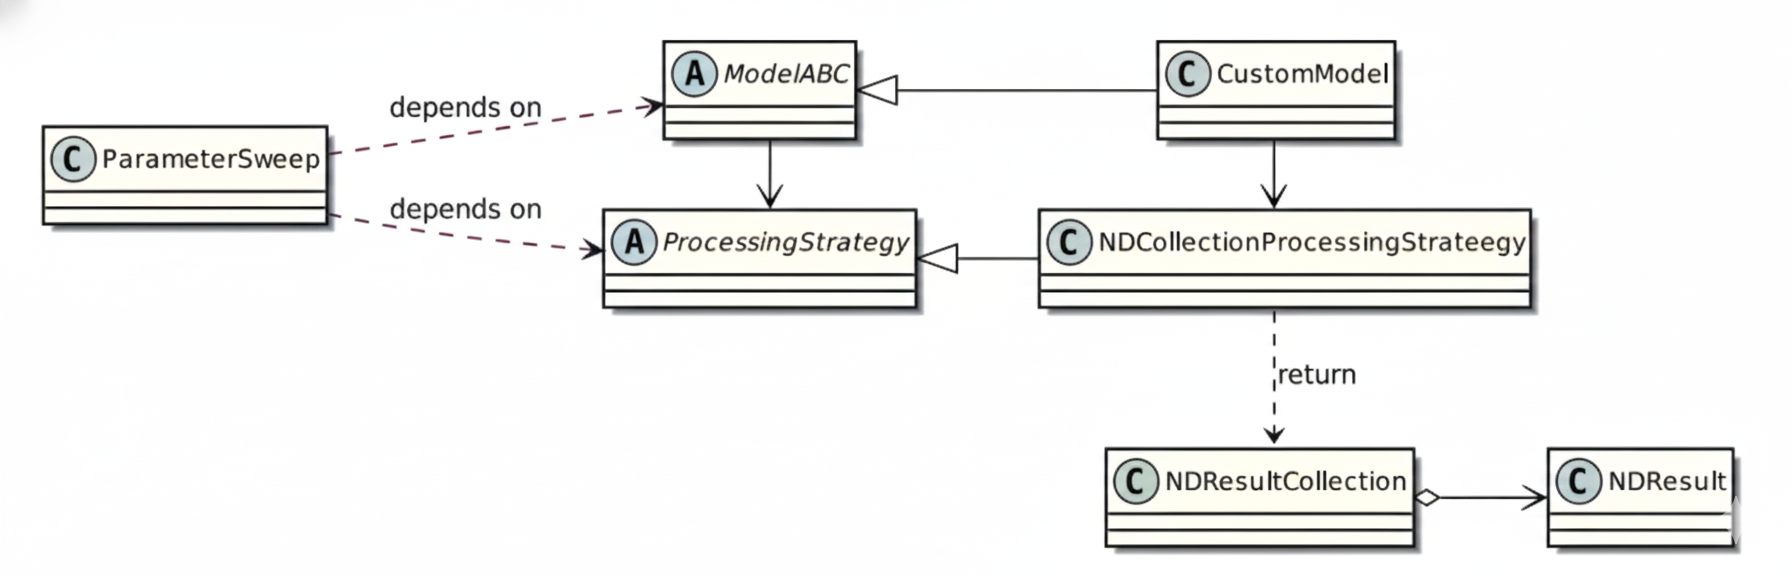
\includegraphics[width=0.95\textwidth]{06_neuromsi/figures/arqui-neuromsi.png}
    \caption{
        Diagrama de clases reducido de Scikit-NeuroMSI. Las flechas vacías representan la herencia, la flecha con punta de diamante indica que varios objetos NDResult se agregan en una única NDResultCollection, y todas las demás relaciones tienen etiquetas explicativas.
    }
    \label{fig:feed-forward}
\end{figure}

\subsection{Backend de datos}
\label{subsec:snmsi_backend}

El almacenamiento y manipulación de datos multidimensionales se implementa mediante \textbf{XArray}\footnote{\url{https://docs.xarray.dev/en/stable/}}, una biblioteca de Python diseñada específicamente para trabajar con arreglos etiquetados de N dimensiones. Esta extiende las capacidades de NumPy agregando nombres y coordenadas a cada dimensión, lo que facilita la selección, agregación y visualización de datos complejos.

Para la persistencia de datos, el framework utiliza un formato basado en archivos ZIP que combina \acrfull{NetCDF} para los datos multidimensionales con JSON para los metadatos. Los resultados de simulaciones se guardan en archivos con extensión \textbf{.ndr} (\textit{NDResult}) o \textbf{.ndc} (\textit{NDResultCollection}). Internamente, cada archivo ZIP contiene: \texttt{metadata.json} con información del modelo, parámetros de ejecución, versión del framework, plataforma y timestamp; y \texttt{nddata.nc} con los datos xarray en formato NetCDF. Esta estructura permite que los resultados sean cargados y analizados posteriormente, compartidos entre investigadores, o procesados con herramientas externas compatibles con NetCDF.


% =============================================================================
% SECCIÓN 3: MODELOS IMPLEMENTADOS
% =============================================================================

\section{Modelos implementados}
\label{sec:snmsi_modelos}

El framework incluye implementaciones de referencia de varios modelos establecidos en la literatura de integración multisensorial. Estas implementaciones sirven tanto como herramientas de investigación como ejemplos para desarrolladores que deseen agregar nuevos modelos.

\medskip
El \textbf{integrador bimodal óptimo} óptimo implementa la combinación de señales mediante máxima verosimilitud según la Ecuación~\ref{eq:mle_integration}. Este modelo asume que ambas señales sensoriales provienen de la misma fuente y las combina ponderando por sus confiabilidades relativas (inversas de las varianzas).

La implementación permite especificar las varianzas de las señales visual y auditiva, ya sea como valores fijos o como funciones de la posición espacial (capturando, por ejemplo, la menor precisión auditiva en la periferia). El modelo proporciona una línea base teórica contra la cual comparar modelos más complejos.

% \subsection{Inferencia causal bayesiana}
% \label{subsec:snmsi_bayesiana}
\medskip
El modelo de \textbf{inferencia causal bayesiana} implementa el marco de \citet{kording2007causal} para inferir la estructura causal subyacente a las señales multisensoriales. A diferencia del integrador MLE, este modelo no asume automáticamente que las señales provienen de la misma fuente, sino que computa la probabilidad posterior de causa común versus causas separadas.

La implementación incluye el cálculo de la probabilidad de causa común, el promediado bayesiano sobre estructuras causales \acrfull{BMA}, y la generación de respuestas de sesgo de localización y juicio de unidad. Los parámetros ajustables incluyen la probabilidad prior de causa común y las varianzas sensoriales.

\medskip
El \textbf{modelo de red de Cuppini} proporciona una implementación completa de la arquitectura de tres capas descrita en la Sección~\ref{sec:modelo_cuppini}. Esta implementación permite simular la dinámica temporal del modelo, variando parámetros como los pesos de conexiones cross-modales, la amplitud de las conexiones laterales tipo sombrero mexicano, y las constantes de tiempo de las diferentes capas.

La implementación soporta la presentación de estímulos audiovisuales con disparidades espaciales y temporales configurables, y extrae predicciones sobre el efecto ventrílocuo (sesgo de localización auditiva) y la inferencia causal (número de picos en la capa multisensorial).


% \subsection{Red de inferencia causal espacio-temporal}
% \label{subsec:snmsi_espaciotemporal}
\medskip
El modelo de \textbf{red de inferencia causal espacio-temporal} extiende la red de Cuppini para incorporar disparidades temporales además de espaciales. Permite estudiar la ventana de integración temporal, es decir, el rango de asincronías audiovisuales dentro del cual los estímulos se perciben como provenientes de una fuente común.

La implementación incluye filtros temporales diferenciados para las modalidades visual y auditiva, capturando las diferentes latencias de procesamiento. Esto permite simular fenómenos como la ilusión del flash inducido por sonido (\textit{sound-induced flash illusion}), donde un único flash acompañado de múltiples sonidos se percibe como múltiples flashes.


% El modelo de \textbf{red de inferencia causal espacio-temporal} extiende el modelo de Cuppini para incorporar disparidades temporales además de espaciales, permitiendo estudiar la ventana de integración temporal y el impacto de la asincronía audiovisual.


% =============================================================================
% SECCIÓN 5: IMPLEMENTACIÓN TÉCNICA
% =============================================================================

\section{Implementación técnica}
\label{sec:snmsi_implementacion}

Esta sección describe aspectos técnicos de la implementación relevantes para desarrolladores que deseen extender el framework o comprender su funcionamiento interno.

\subsection{Ejecución paralela}
\label{subsec:snmsi_paralelo}

Para barridos de parámetros extensos, el framework soporta ejecución paralela mediante el módulo \texttt{multiprocessing} de Python. El usuario puede especificar el número de procesos a utilizar, y el framework distribuye automáticamente las simulaciones entre ellos.

Para modelos implementados con JAX, la paralelización puede extenderse a GPUs mediante \texttt{jax.pmap}, permitiendo ejecutar múltiples simulaciones simultáneamente en dispositivos de alto rendimiento.

\subsection{Gestión de memoria}
\label{subsec:snmsi_memoria}

Los modelos de redes neuronales con dinámica temporal pueden generar grandes volúmenes de datos (actividad de cientos de neuronas durante miles de pasos temporales en múltiples trials). El framework implementa estrategias para manejar estos casos: almacenamiento incremental a disco durante simulaciones largas, compresión de datos y opciones para almacenar solo estadísticas resumidas en lugar de trayectorias completas.

% =============================================================================
% SECCIÓN 6: APLICACIONES
% =============================================================================

\section{Aplicaciones}
\label{sec:snmsi_aplicaciones}

En el artículo que presenta el framework, \citet{paredes2025scikit} demuestran su utilidad mediante varios análisis representativos.

\subsection{Paradigma del efecto ventrílocuo}
\label{subsec:snmsi_ventrilocuo}

El efecto ventrílocuo, introducido en la Sección~\ref{subsec:ventriloquismo}, constituye el paradigma principal para validar modelos de integración audiovisual. El framework permite simular experimentos típicos donde estímulos visual y auditivo se presentan con diferentes disparidades espaciales, midiendo el sesgo resultante en la localización auditiva percibida.

Un ejemplo típico de uso del framework para simular el efecto ventrílocuo es:

\begin{code}
\begin{minted}{pycon}
>>> from skneuromsi.neural import Cuppini2017
>>> from skneuromsi import ParameterSweep
>>> import numpy as np

# Crear modelo con modalidades específicas
>>> model = Cuppini2017(mode0="auditory", mode1="visual")

# Configurar barrido de disparidades
>>> disparities = np.arange(-24, 25, 6)
>>> sweep = ParameterSweep(
    model=model,
    target="visual_position",
    range=45 + disparities
)

# Ejecutar simulaciones
>>> results = sweep.run(auditory_position=45)

# Visualizar resultados
>>> results.cplot.unity_report()
\end{minted}
\caption{
    Ejemplo del uso de Scikit-NeuroMSI para simular el efecto ventrílocuo. Se crea un modelo Cuppini2017 con modalidades auditiva y visual, se configura un barrido de disparidades espaciales, y se visualizan los resultados mediante el accessor de colección.
}
\label{code:usage}
\end{code}
\vspace{1.5em}


Los autores comparan las predicciones de modelos bayesianos y de redes neuronales, encontrando que ambos reproducen cualitativamente el patrón experimental de sesgo decreciente con la disparidad, pero con diferencias cuantitativas que podrían distinguirse experimentalmente.

\subsection{Ilusión del flash inducido por sonido}
\label{subsec:snmsi_flash}

Esta ilusión, donde un único flash visual acompañado de múltiples sonidos se percibe como múltiples flashes, demuestra que la integración multisensorial puede alterar la percepción incluso de modalidades típicamente dominantes como la visión. El modelo de red de inferencia causal espacio-temporal, desarrollado por el grupo de investigación de los autores del framework, fue construido específicamente para dar cuenta de este fenómeno \citep{paredes2025scikit}.


\subsection{Aplicaciones clínicas}
\label{subsec:snmsi_clinicas}

Los autores señalan que una aplicación prometedora del framework es el estudio de diferencias en integración multisensorial asociadas a condiciones psiquiátricas y neurológicas. Estudios han documentado alteraciones en la integración audiovisual en trastornos del espectro autista (TEA), esquizofrenia, y demencias. El framework permitiría formalizar hipótesis sobre qué parámetros de los modelos podrían estar alterados en estas condiciones, y generar predicciones cuantitativas testables experimentalmente.

% =============================================================================
% SECCIÓN 7: COMPARACIÓN CON OTROS FRAMEWORKS
% =============================================================================

\section{Contexto en el ecosistema de herramientas}
\label{sec:snmsi_contexto}

Scikit-NeuroMSI ocupa un nicho específico en el ecosistema de herramientas para neurociencia computacional. A diferencia de simuladores de redes neuronales de propósito general como \textbf{Brian}\footnote{\url{https://briansimulator.org/}} o \textbf{NEST}\footnote{\url{https://ebrains.eu/data-tools-services/tools/nest}}, que se enfocan en la simulación detallada de neuronas de disparo, Scikit-NeuroMSI está diseñado específicamente para modelos de integración multisensorial, proporcionando abstracciones y herramientas optimizadas para este dominio.

Comparado con frameworks de modelado cognitivo como \textbf{HDDM}\footnote{\url{https://hddm.readthedocs.io/}} (para modelos de difusión de decisiones) o \textbf{TAPAS}\footnote{\url{https://www.translationalneuromodeling.org/tapas}} (para modelos computacionales en psiquiatría), Scikit-NeuroMSI se especializa en la dimensión sensorial del procesamiento, permitiendo una descripción más detallada de cómo señales de múltiples modalidades se combinan antes de informar decisiones.

Frameworks de redes neuronales recurrentes como \textbf{PyRates}\footnote{\url{https://pyrates.readthedocs.io/}} o \textbf{BrainPy}\footnote{\url{https://brainpy.readthedocs.io/}} comparten el enfoque en dinámicas de poblaciones neuronales, pero no incluyen las abstracciones específicas para estímulos multisensoriales, inferencia causal, o métricas de integración que Scikit-NeuroMSI proporciona.

% =============================================================================
% SECCIÓN 8: DIRECCIONES FUTURAS Y CONTRIBUCIONES
% =============================================================================

\section{Direcciones futuras y contribuciones de la comunidad}
\label{sec:snmsi_futuro}

El desarrollo de Scikit-NeuroMSI continúa activamente, con varias direcciones planificadas para versiones futuras.

% \begin{enumerate}
%     \item
\subsubsection{Mejoras arquitectónicas}
\label{subsec:snmsi_mejoras}

Una mejora planificada es la separación más clara entre la representación de estímulos y los integradores que los procesan. Actualmente, algunos modelos asumen formatos específicos de estímulo, lo que limita la flexibilidad. Una arquitectura de ``estímulo-integrador'' más modular permitiría combinar diferentes tipos de estímulos con diferentes modelos de manera más flexible.

Otra dirección es el soporte mejorado para modelos jerárquicos, donde la salida de un modelo alimenta la entrada de otro. Esto permitiría construir arquitecturas complejas combinando componentes más simples.

\subsubsection{Nuevos modelos}
\label{subsec:snmsi_nuevos_modelos}

El framework está diseñado para que la comunidad contribuya nuevas implementaciones de modelos. Dando lugar al presente trabajo que contribuye en esta dirección mediante la implementación del modelo de Echeveste, que introduce al framework el primer modelo con dinámicas corticales realistas basadas en muestreo estocástico. Esta implementación establece patrones para que futuros contribuidores puedan seguir para agregando modelos similares.

\subsubsection{Información del proyecto}
\label{subsec:snmsi_info}

Scikit-NeuroMSI se distribuye bajo licencia BSD 3-Clause, permitiendo uso libre tanto académico como comercial. El código fuente está disponible en GitHub\footnote{\url{https://github.com/renatoparedes/scikit-neuromsi}}, donde se aceptan contribuciones mediante pull requests. La documentación completa, incluyendo tutoriales y referencia de API, está disponible en Read the Docs\footnote{\url{https://scikit-neuromsi.readthedocs.io}}.

% =============================================================================
% SECCIÓN 9: RELEVANCIA PARA EL PRESENTE TRABAJO
% =============================================================================

\section{Relevancia para el presente trabajo}
\label{sec:snmsi_relevancia}

Scikit-NeuroMSI proporciona la infraestructura técnica fundamental sobre la cual se desarrolla la implementación del modelo de Echeveste presentada en esta tesis. Específicamente:

La implementación existente del modelo de Cuppini sirve como \textbf{punto de referencia} para entender cómo modelos de redes neuronales se integran en el framework, y como objetivo eventual para futuras extensiones que combinen ambos enfoques.

La arquitectura modular del framework permite \textbf{integrar} el modelo de Echeveste de manera que pueda ser comparado directamente con modelos existentes usando las mismas herramientas de análisis.

Las abstraccion de NDResult proporciona una \textbf{estructura natural} para almacenar las trayectorias temporales de potenciales de membrana que el modelo de Echeveste genera, con soporte para múltiples trials, condiciones de estímulo, y poblaciones neuronales.

Las herramientas de visualización y análisis existentes pueden \textbf{extenderse} para las necesidades específicas del modelo de Echeveste, como análisis espectral para detectar oscilaciones gamma o comparación de momentos de respuesta con momentos objetivo.

Finalmente, al contribuir la implementación del modelo de Echeveste al framework, este trabajo la hace \textbf{disponible para la comunidad científica}, maximizando su impacto y reproducibilidad, y estableciendo las bases para que otros investigadores construyan sobre este trabajo hacia modelos de integración multisensorial con dinámicas corticales realistas. \cleardoublepage
\chapter{Implementación}
\label{chapter:implementacion}

Este capítulo describe la implementación del modelo de \citeauthor{echeveste2020cortical} dentro del framework Scikit-NeuroMSI. La implementación abarca desde la arquitectura de software hasta los algoritmos de optimización, pasando por el modelo generativo \acrshort{GSM}, las dinámicas de la red \acrshort{SSN}, y los módulos de soporte desarrollados.

El código fuente se estructura siguiendo los principios de diseño del framework, lo que permite que el modelo se integre naturalmente con los existentes y pueda beneficiarse de las herramientas de análisis y comparación ya implementadas. A lo largo del capítulo presentamos las decisiones de diseño tomadas, las equivalencias con el código original, y las justificaciones basadas en el artículo original. La Tabla~\ref{tab:parametros_completos}, presentada al final del capítulo, consolida todos los parámetros del modelo como referencia técnica.

% =============================================================================
% SECCIÓN 1: ARQUITECTURA GENERAL
% =============================================================================

\section{Arquitectura general de la implementación}
\label{sec:impl_arquitectura}

La implementación del modelo de Echeveste se estructuró en varios módulos interconectados que separan responsabilidades siguiendo el principio de responsabilidad única. Esta organización facilita el mantenimiento, las pruebas unitarias, y permite futuras extensiones de manera modular.

\subsection{Estructura de módulos}
\label{subsec:impl_modulos}

El código está organizado en cinco archivos principales dentro del paquete \texttt{skneuromsi/\-neural/\-echeveste2020}, cada uno con responsabilidades claramente delimitadas (para una visión detallada de la organización modular y las dependencias entre archivos, véase la Figura~\ref{fig:component-diagram}:

\begin{itemize}
    \item \textbf{\texttt{\_model.py}}: contiene la clase principal \texttt{Echeveste2020} que implementa el modelo completo, incluyendo el entrenamiento en dos etapas descrito en la Sección~\ref{subsec:echeveste_entrenamiento}, la simulación de dinámicas neuronales según la Ecuación~\ref{eq:ssn_dynamics}, y la construcción de matrices de conectividad parametrizadas según la Ecuación~\ref{eq:weight_parametrization}. Este archivo también define la clase \texttt{SSNIntegrator}, que encapsula la integración numérica de las ecuaciones diferenciales.

    \item \textbf{\texttt{\_training.py}}: implementa las funciones de entrenamiento utilizando JAX para diferenciación automática. Aquí se encuentra el cálculo de momentos no lineales necesarios para la activación supralineal, la evolución temporal de los momentos mediante el método \acrshort{ADF}, y la función de costo con sus cuatro términos según la Ecuación~\ref{eq:cost_function}.

    \item \textbf{\texttt{\_gsm.py}}: define la clase \texttt{GSM} que implementa el modelo generativo de mezcla de escala gaussiana. Su función principal es generar los inputs externos $\mathbf{h}$ para la red SSN a partir de estímulos visuales, aplicando la transformación no lineal de la Ecuación~\ref{eq:feedforward_input}. También permite generar estímulos sintéticos y calcular los momentos objetivo que sirven como targets durante el entrenamiento.

    \item \textbf{\texttt{\_visualization.py}}: proporciona funciones de visualización especializadas para analizar las dinámicas del modelo, incluyendo potenciales de membrana, tasas de disparo, espectros de potencia, y análisis de transitorios.

    \item \textbf{\texttt{\_data\_loader.py}}: proporciona acceso a los parámetros pre-entrenados por los autores originales, permitiendo cargar configuraciones validadas sin necesidad de ejecutar el costoso proceso de optimización.
\end{itemize}

La Figura~\ref{fig:impl_clases} presenta el diagrama de clases UML que ilustra las relaciones entre los componentes principales. La clase \texttt{Echeveste2020} hereda de la clase base abstracta del framework \texttt{SKNMSIMethodABC}, lo que garantiza compatibilidad con las herramientas de análisis existentes. Esta clase compone un integrador \texttt{SSNIntegrator} para resolver las ecuaciones diferenciales, utiliza el modelo generativo \texttt{GSM} durante el entrenamiento para calcular los momentos objetivo, y produce resultados en formato \texttt{NDResult} compatible con el ecosistema del framework.

\begin{figure}[H]
    \centering
    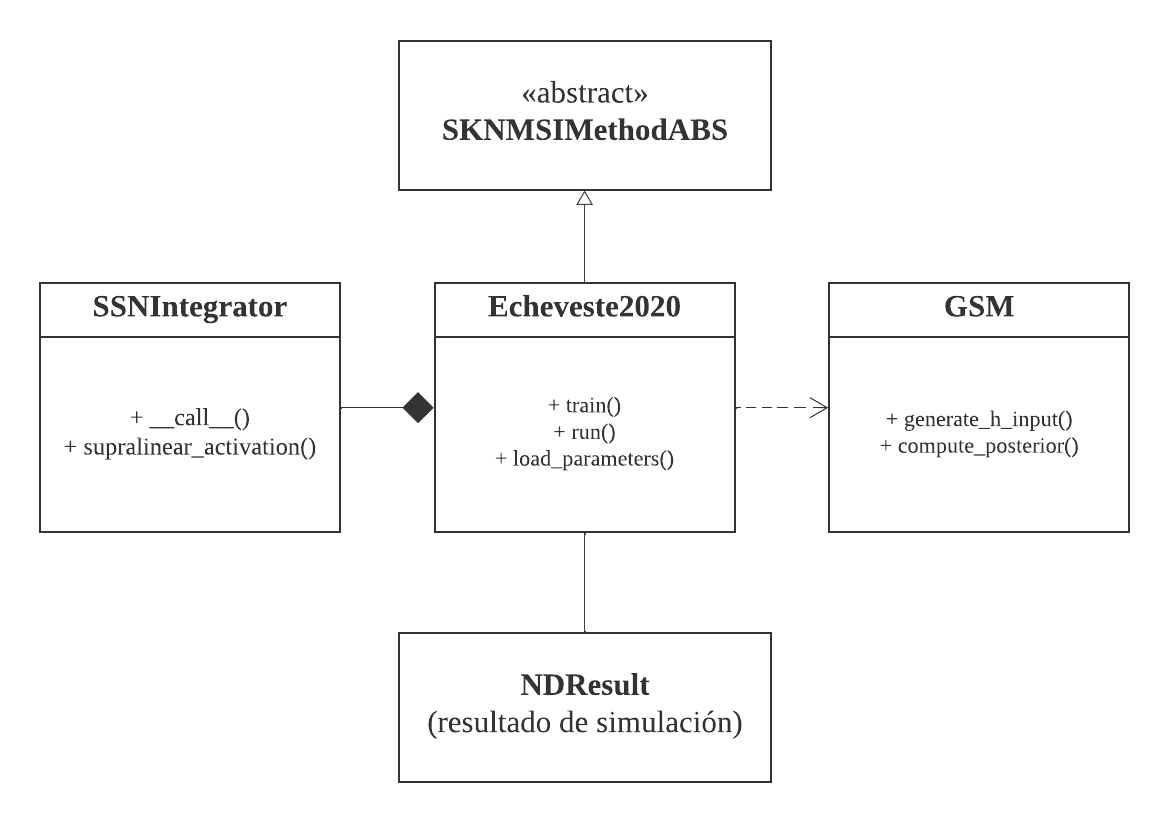
\includegraphics[width=0.8\textwidth]{07_implementacion/figures/DiagramaUML.png}
    \caption{Diagrama de clases UML simplificado de la implementación del modelo de Echeveste. Para una versión detallada, véase la Figura~\ref{fig:class-diagram}.}
    \label{fig:impl_clases}
\end{figure}

\subsection{Inicialización y configuración}
\label{subsec:impl_inicializacion}

El modelo por defecto se inicializa con parámetros nulos que deben ser optimizados antes de poder realizar inferencia. En este caso, el usuario debe invocar el método \texttt{train()} para ejecutar el procedimiento de optimización en dos etapas, o bien llamar al método \texttt{load\_parameters()} para cargar los parámetros pre-optimizados posteriormente. Una vez configurado el modelo, el método \texttt{run()} ejecuta la simulación de las dinámicas neuronales dado un estímulo especificado, retornando un objeto \texttt{NDResult} compatible con las herramientas de análisis del framework. El flujo completo de inicialización, entrenamiento y simulación se ilustra en detalle en el diagrama de secuencia en la Figura~\ref{fig:sequence-training-full}.

Otra opción es pasar el parámetro \texttt{pretrained=True} durante la construcción, esto cargará automáticamente los parámetros pre-optimizados por los autores originales, quedando listo para ejecutar simulaciones inmediatamente. Esta opción resulta conveniente para los usuarios que desean explorar el comportamiento del modelo sin invertir tiempo en el proceso de optimización.


% =============================================================================
% SECCIÓN 2: EL MODELO GENERATIVO GSM
% =============================================================================

\section{Implementación del modelo generativo}
\label{sec:impl_gsm}

El modelo generativo \acrshort{GSM} define el problema de inferencia que la red \acrshort{SSN} debe resolver. Desde el punto de vista de la implementación, cumple dos funciones esenciales: proporciona los estímulos de entrada transformados al espacio de la red neuronal y calcula los momentos objetivo contra los cuales se evalúa el desempeño durante el entrenamiento.

\subsection{Clase GSM y sus responsabilidades}
\label{subsec:impl_gsm_clase}

La clase \texttt{GSM} encapsula el modelo generativo descrito en la Sección~\ref{subsec:echeveste_gsm}. Sus responsabilidades principales incluyen la generación de filtros de Gabor que constituyen la matriz de campos proyectivos $\mathbf{A}$, la producción de parches de imagen con diferentes niveles de contraste según la Ecuación~\ref{eq:gsm}, el cálculo de la media y covarianza de la distribución posterior $P(\mathbf{y}|\mathbf{x}, z)$ según las Ecuaciones~\ref{eq:target_mean} y \ref{eq:target_cov}, y la aplicación de la transformación no lineal que convierte la proyección del estímulo en la entrada feedforward de las neuronas.

Una decisión de diseño importante fue separar la lógica del modelo generativo en una clase independiente, en lugar de integrarla directamente en la clase principal del modelo neuronal. Esta separación permite reutilizar el GSM en otros contextos, facilita las pruebas unitarias de cada componente, y refleja la distinción conceptual entre el problema computacional (definido por el GSM) y su implementación neuronal (la red SSN).

\subsection{Transformación de entrada feedforward}
\label{subsec:impl_gsm_h}

La transformación que convierte un parche de imagen $\mathbf{x}$ en la entrada feedforward $\mathbf{h}$ de la red neuronal es un punto crucial en nuestra implementación, siguiendo la Ecuación~\ref{eq:feedforward_input}. Esta transformación involucra tres parámetros optimizables ($\alpha_h$, $\beta_h$, $\gamma_h$) cuyos valores finales se presentan en la Tabla~\ref{tab:parametros_completos}.

La implementación sigue fielmente la formulación matemática, aplicando secuencialmente la proyección lineal mediante los pesos feedforward, el desplazamiento por la línea base, la rectificación, la potenciación, y finalmente el escalado. El valor del exponente $\gamma_h \approx 2$ resulta notablemente similar al exponente supralineal $n = 2$ utilizado en la función de transferencia de las neuronas, lo que sugiere una consistencia en el procesamiento no lineal a través del modelo.

% =============================================================================
% SECCIÓN 3: EL INTEGRADOR SSN
% =============================================================================

\section{Implementación del integrador SSN}
\label{sec:impl_ssn}

La base computacional del modelo es el integrador de la red supralineal estabilizada \acrshort{SSN}, que implementa las ecuaciones diferenciales que rigen la dinámica de los potenciales de membrana según la Ecuación~\ref{eq:ssn_dynamics}.

\subsection{Diseño de la clase}
\label{subsec:impl_ssn_integrador}

La clase \texttt{SSNIntegrator} se implementa como un \textit{dataclass} de Python que encapsula las ecuaciones diferenciales del modelo. Esta decisión de diseño tiene varias ventajas: permite que el mismo integrador sea reutilizado tanto durante el entrenamiento como durante la simulación, facilita su uso con el framework BrainPy para integración numérica, y hace explícitos los parámetros del modelo como atributos inmutables de la clase.

Los atributos de la clase corresponden a las constantes temporales de las poblaciones neuronales ($\tau_E$, $\tau_I$, $\tau_\eta$) y a los parámetros de la función de transferencia supralineal ($n$, $k$). Todos estos valores se mantienen fijos durante el entrenamiento según los valores de la Tabla~\ref{tab:parametros_completos}.

\subsection{Función de activación y ecuaciones dinámicas}
\label{subsec:impl_ssn_dynamics}

La función de transferencia supralineal convierte los potenciales de membrana en tasas de disparo según la Ecuación~\ref{eq:firing_rate}. La implementación utiliza el backend matemático de BrainPy, que permite ejecución transparente en GPU cuando está disponible, proporcionando aceleración significativa para simulaciones largas.

El método principal del integrador computa las derivadas temporales de los potenciales de membrana, manejando correctamente la estructura de bloques de la matriz de conectividad. Una consideración importante en la implementación es el respeto del principio de Dale: los signos de las conexiones están incorporados directamente en la matriz $\mathbf{W}$, de modo que las conexiones desde neuronas excitatorias son siempre positivas y las conexiones desde neuronas inhibitorias son siempre negativas.

% =============================================================================
% SECCIÓN 4: CONECTIVIDAD PARAMÉTRICA
% =============================================================================

\section{Conectividad paramétrica}
\label{sec:impl_conectividad}

Una característica distintiva del modelo de Echeveste es la parametrización circulante de la matriz de conectividad, que reduce drásticamente el número de parámetros libres respetando la simetría rotacional de la topología de anillo.

La matriz de conectividad $\mathbf{W}$ se construye a partir de solo 8 parámetros según la Ecuación~\ref{eq:weight_parametrization}. Esta parametrización reducida constituye una decisión de diseño fundamental del modelo. Con 100 neuronas en la red (50 excitatorias y 50 inhibitorias), una matriz de conectividad sin restricciones contendría 10,000 pesos sinápticos independientes. Optimizar tantos parámetros simultáneamente presentaría múltiples dificultades: el espacio de búsqueda sería enorme, el riesgo de sobreajuste a los estímulos de entrenamiento sería elevado, y el costo computacional de calcular gradientes para cada peso haría el entrenamiento impracticable.

La parametrización circulante resuelve estos problemas al explotar la simetría rotacional inherente a la topología de anillo. Dado que las neuronas están organizadas según su orientación preferida, resulta biológicamente plausible asumir que la fuerza de conexión entre dos neuronas depende únicamente de la diferencia entre sus orientaciones, no de sus valores absolutos. Esta suposición reduce drásticamente los grados de libertad: cada bloque de la matriz queda completamente determinado por solo dos parámetros, una amplitud $a$ y un ancho $d$, que definen un kernel gaussiano circular.

Cada uno de los cuatro bloques de la matriz ($\mathbf{W}_{EE}$, $\mathbf{W}_{EI}$, $\mathbf{W}_{IE}$, $\mathbf{W}_{II}$) se genera aplicando este kernel a las diferencias de orientación entre neuronas presinápticas y postsinápticas. El resultado es una matriz con estructura de banda: las conexiones son más fuertes entre neuronas con orientaciones similares y decaen suavemente para orientaciones distantes. Los valores optimizados de estos parámetros se presentan en la Tabla~\ref{tab:parametros_completos}.

La implementación construye cada bloque de manera vectorizada para mayor eficiencia computacional, evitando bucles explícitos sobre pares de neuronas. Esta vectorización resulta esencial dado que la construcción de la matriz debe realizarse múltiples veces durante el proceso de optimización, cada vez que se actualizan los parámetros de conectividad.

% =============================================================================
% SECCIÓN 5: PROCESO DE ENTRENAMIENTO
% =============================================================================

\section{Proceso de entrenamiento}
\label{sec:impl_entrenamiento}

El entrenamiento del modelo sigue el procedimiento de optimización en dos etapas descrito en la Sección~\ref{subsec:echeveste_entrenamiento}. La implementación utiliza JAX para diferenciación automática, combinando los optimizadores Optax (Stage 1) y SciPy (Stage 2). Para una visualización completa de las interacciones entre componentes durante ambas etapas de optimización, incluyendo el flujo de datos y las llamadas a funciones específicas, véase la Figura~\ref{fig:sequence-training-full}.

\subsection{Stage 1: Optimización estocástica con ADAM}
\label{subsec:impl_stage1}

La primera etapa utiliza el optimizador \acrshort{ADAM} con estimación estocástica de los momentos de respuesta. Los hiperparámetros de esta etapa están presentados en la siguiente tabla.

\begin{table}[H]
\centering
\caption{Hiperparámetros de optimización Stage 1.}
\label{tab:stage1_params}
\begin{tabular}{llc}
\toprule
\textbf{Parámetro} & \textbf{Descripción} & \textbf{Valor} \\
\midrule
$\eta$ & Tasa de aprendizaje ADAM & 0.002 \\
$\beta_1$ & Momento de primer orden & 0.9 \\
$\beta_2$ & Momento de segundo orden & 0.999 \\
$N_\text{trial}$ & Trials por iteración & 50 \\
Iteraciones & Número de pasos ADAM & 250 \\
\bottomrule
\end{tabular}
\end{table}

Una característica importante del Stage 1 es el  \textit{annealing} del tiempo inicial de integración $T_{\min}$, que comienza en 0 ms y aumenta progresivamente hasta $T_{\max} - 50$ ms a lo largo de las iteraciones. Este esquema de  \textit{curriculum learning} incentiva que la red aprenda dinámicas de muestreo rápidas desde el inicio del estímulo, evitando soluciones que solo convergen lentamente hacia los momentos objetivo.

\subsection{Stage 2: Optimización determinística con L-BFGS-B}
\label{subsec:impl_stage2}

La segunda etapa optimiza los 15 parámetros totales utilizando el optimizador quasi-Newton \acrshort{L-BFGS-B} con el método \acrshort{ADF} para calcular determinísticamente los momentos de respuesta. A diferencia del método estocástico de Stage 1 que puede tener alta varianza en las estimaciones, \acrshort{ADF} proporciona gradientes exactos (bajo la aproximación gaussiana) que permiten una convergencia más precisa.

Los parámetros adicionales optimizados en Stage 2 incluyen los 3 parámetros de la transformación de entrada ($\alpha_h$, $\beta_h$, $\gamma_h$) y los 4 parámetros de la covarianza de ruido ($\sigma_E$, $\sigma_I$, $\rho$, $d_\sigma$), cuyos valores óptimos se encuentran en la Tabla~\ref{tab:parametros_completos}.

\subsection{Función de costo}
\label{subsec:impl_costo}

La función de costo implementa la Ecuación~\ref{eq:cost_function}, penalizando diferencias entre los momentos de la distribución de respuestas de la red y los momentos objetivo del \acrshort{GSM}. Los pesos relativos de cada término, presentados en la siguiente tabla, fueron ajustados por los autores originales para balancear la contribución de cada componente.

\begin{table}[H]
\centering
\caption{Pesos de la función de costo.}
\label{tab:cost_weights}
\begin{tabular}{llc}
\toprule
\textbf{Peso} & \textbf{Término} & \textbf{Valor} \\
\midrule
$\epsilon_\mu$ & Error de media & $4.0 \times 10^{-5}$ \\
$\epsilon_\sigma$ & Error de varianza & $8.0 \times 10^{-5}$ \\
$\epsilon_\Sigma$ & Error de covarianza & $8.0 \times 10^{-7}$ \\
$\epsilon_{\text{slow}}$ & Penalización de lentitud & $4.0 \times 10^{-10}$ \\
\bottomrule
\end{tabular}
\end{table}

El término de \textit{slowness} penaliza la autocorrelación temporal de las respuestas, incentivando que muestras consecutivas sean estadísticamente independientes. Sin este término, la red podría aprender a producir los momentos correctos pero con dinámicas temporales excesivamente lentas que harían el muestreo ineficiente.

\subsection{Reimplementación en JAX}
\label{subsec:impl_jax}

Uno de los desafíos inesperados de este trabajo fue descubrir que el código de entrenamiento original de \citet{echeveste2020cortical} estaba implementado en OCaml\footnote{\url{https://ocaml.org/}}, un lenguaje de programación funcional que resulta completamente atípico para el desarrollo de modelos de redes neuronales en la actualidad. La comunidad de neurociencia computacional y aprendizaje automático ha convergido casi universalmente hacia Python como lenguaje de implementación, con frameworks como TensorFlow\footnote{\url{https://www.tensorflow.org/}}, PyTorch\footnote{\url{https://pytorch.org/}} o JAX\footnote{\url{https://docs.jax.dev/}} como herramientas estándar para diferenciación automática y cómputo en \acrshort{GPU}. Encontrar una implementación en OCaml representó un obstáculo considerable que requirió una adaptación drástica de nuestra estrategia de desarrollo.

En comunicación personal con el Dr. Echeveste, pudimos comprender las razones históricas detrás de esta elección. Dado el momento en que se desarrolló el modelo original (2016), las herramientas de diferenciación automática que hoy consideramos estándar no existían o no habían alcanzado la madurez necesaria para este tipo de aplicaciones. OCaml ofrecía entonces ciertas ventajas para implementar el método \acrshort{ADF}, que requiere propagar gradientes a través de ecuaciones diferenciales de manera eficiente. Sin embargo, esta decisión técnica, perfectamente razonable en su contexto original, dejó el código en un estado de difícil acceso para la comunidad científica actual.

La reimplementación en JAX constituyó, por tanto, no solo una traducción de código sino una actualización tecnológica sustancial del modelo. JAX fue la elección natural por varias razones. En primer lugar, su paradigma de programación funcional (con funciones puras, sin efectos secundarios ni estado mutable) guarda cierta afinidad conceptual con OCaml, lo que facilitó la traducción de las estructuras algorítmicas del código original. Las ecuaciones del modelo pueden expresarse en JAX de forma casi idéntica a su formulación matemática, manteniendo una correspondencia directa con el paper original.

En segundo lugar, JAX ya se encontraba integrado en el framework Scikit-NeuroMSI como dependencia para otros componentes. Esta preexistencia significó que los usuarios del framework no necesitan instalar dependencias adicionales para utilizar el modelo de Echeveste, y que la implementación puede beneficiarse de utilidades y patrones ya establecidos en el código base. Esta coherencia tecnológica dentro del framework simplifica el mantenimiento a largo plazo y facilita futuras integraciones entre modelos.

Desde el punto de vista computacional, JAX ofrece compilación \acrlong{JIT} mediante \acrshort{XLA}\footnote{
La compilación \acrshort{JIT} en JAX se basa en \acrfull{XLA}, un compilador que analiza el grafo completo de operaciones numéricas y produce una versión optimizada del cálculo, adaptada al dispositivo de ejecución, reduciendo el overhead interpretativo y el uso de memoria intermedia.
}
, que optimiza automáticamente las operaciones para el hardware disponible. Esto resulta particularmente beneficioso durante el entrenamiento, donde la función de costo y sus gradientes deben evaluarse cientos de veces. La transformación \texttt{jax.grad} permite obtener gradientes exactos de funciones arbitrarias de manera composicional: si una función $f$ se compone de operaciones diferenciables, su gradiente se obtiene automáticamente sin necesidad de derivar manualmente las expresiones analíticas. Esta capacidad es esencial para el método \acrshort{ADF} utilizado en Stage 2, donde los gradientes deben propagarse a través de la evolución temporal de los momentos de la distribución. Además, JAX proporciona soporte transparente para ejecución en \acrshort{GPU}, permitiendo acelerar significativamente tanto el entrenamiento como las simulaciones sin modificar el código.

En definitiva, la reimplementación en JAX transformó un código técnicamente correcto pero prácticamente inaccesible en una implementación moderna, mantenible y compatible con el ecosistema actual de herramientas de neurociencia computacional.

% =============================================================================
% SECCIÓN 6: SIMULACIÓN
% =============================================================================

\section{Simulación de dinámicas neuronales}
\label{sec:impl_simulacion}

Una vez entrenado el modelo (o cargados los parámetros pre-entrenados), el método \texttt{run()} ejecuta la simulación de las dinámicas neuronales. Esta sección describe los modos de simulación disponibles, el proceso de evolución temporal, y la estructura de los resultados.

\subsection{Modos de simulación}
\label{subsec:impl_modos}

La implementación soporta dos modos de simulación que corresponden a diferentes propósitos experimentales del trabajo original.

El \textbf{modo de fase única} (\textit{single-phase}) mantiene el estímulo presente durante toda la simulación. Este modo replica las condiciones utilizadas durante el entrenamiento de la red, donde la función objetivo evalúa las estadísticas de muestreo en estado estacionario. Es el modo apropiado para validar que la red entrenada reproduce correctamente las distribuciones \textit{target} del modelo \acrshort{GSM}, y para análisis de respuestas estacionarias como la sintonización de orientación y la variabilidad neural dependiente del contraste.

El \textbf{modo de tres fases} (\textit{three-phase}) divide la simulación en tres períodos temporales distintos: actividad espontánea pre-estímulo (225 ms por defecto), presentación del estímulo (100 ms), y actividad espontánea post-estímulo (125 ms). Este modo replica las condiciones experimentales del código de simulación original y permite estudiar fenómenos dinámicos que emergen específicamente del entrenamiento basado en muestreo: los \textit{overshoots} transitorios al inicio del estímulo, las dinámicas de \textit{onset/offset}, y las oscilaciones gamma moduladas por el estímulo.

El modo de tres fases soporta opcionalmente \textbf{delays por neurona} en las transiciones de estímulo, modelando la variabilidad temporal con que diferentes neuronas reciben la señal de entrada. Los delays se muestrean de una distribución normal con media de 45 ms y desviación estándar de 5 ms (valores por defecto del código original). Esta característica permite simular las condiciones utilizadas en el paper para analizar los \textit{overshoots} promediados sobre múltiples configuraciones de \textit{delay}.

La distinción entre ambos modos refleja un hallazgo central del trabajo original: aunque el entrenamiento optimiza para estado estacionario (modo single-phase), la red emergente exhibe dinámicas transitorias funcionalmente relevantes (modo three-phase). Los \textit{overshoots} al \textit{onset} del estímulo no son defectos sino características funcionales que mejoran la inferencia continua, compensando el sesgo introducido por promediar respuestas sobre ventanas temporales finitas \citep{echeveste2020cortical}.

\subsection{Evolución temporal e integración numérica}
\label{subsec:impl_evolucion}

El proceso de simulación consta de dos etapas: un período de estabilización inicial seguido del registro de actividad. La integración de las ecuaciones diferenciales (Ecuación~\ref{eq:ssn_dynamics}) utiliza el método de Euler explícito con paso de tiempo $dt = 0.2$ ms, consistente con el código original. El framework BrainPy proporciona la infraestructura de integración:

\begin{code}
\begin{minted}{python}
# Initialize BrainPy ODE integrator
integrator_model = SSNIntegrator(
    tau_e=0.020,  # 20 ms in seconds
    tau_i=0.010,  # 10 ms in seconds
    tau_n=0.020,  # 20 ms in seconds
    n=2.0, k=0.3
)
self._integrator = bp.odeint(f=integrator_model, method='euler', dt=0.2e-3)
\end{minted}
\caption{Inicialización del integrador numérico con BrainPy.}
\label{code:brainpy_integrator}
\end{code}
\vspace{1.5em}

La primera etapa es el período de \textbf{\textit{burn-in}}, durante el cual la red evoluciona sin registrar datos. Este período es necesario porque las condiciones iniciales (potenciales de membrana y ruido) se inicializan de manera arbitraria, y la red requiere tiempo para alcanzar el régimen estacionario estocástico desde el cual las muestras son representativas de la distribución posterior. El valor por defecto de 10,000 ms corresponde al utilizado en el código original, aunque para experimentos de transitorios se recomienda aumentarlo a 20,000 ms.

Durante tanto el burn-in como la simulación principal, el ruido de inferencia $\boldsymbol{\eta}$ evoluciona según un proceso que mantiene la estructura de correlaciones espaciales definida por la matriz $\boldsymbol{\Sigma}_\eta$:

\begin{code}
\begin{minted}{python}
def _update_noise(self, eta_old, L, dt, tau_n):
    """Update noise via Ornstein-Uhlenbeck process.
    
    η(t+dt) = η(t)·(1 - dt/τ_η) + √(2·dt/τ_η)·L·ξ
    where ξ ~ N(0,I) and L is Cholesky factor of Σ_η.
    """
    eps_1 = 1.0 - dt / tau_n
    eps_2 = np.sqrt(2.0 * dt / tau_n)
    xi = self._random.standard_normal(self._N)
    return eps_1 * eta_old + eps_2 * (L @ xi)
\end{minted}
\caption{Actualización del ruido correlacionado.}
\label{code:ou_noise}
\end{code}
\vspace{1.5em}

El loop principal de simulación alterna entre la actualización del ruido y la integración de las dinámicas neuronales, determinando el estímulo apropiado en cada paso según el modo de simulación y la fase temporal actual.

\subsection{Estructura del resultado}
\label{subsec:impl_resultado}

Una vez completada la evolución temporal, el método \texttt{run()} empaqueta las trayectorias registradas en un objeto \texttt{NDResult}, el formato estándar de resultados del framework. Esto permite que los resultados del modelo de Echeveste sean directamente compatibles con las herramientas de análisis y visualización desarrolladas para otros modelos del framework, facilitando comparaciones y análisis unificados. Pero a su vez, la complejidad de este nuevo modelo impulso el desarrollo de herramientas nuevas para su analisis las cuales se adaptaron y trabajan bajo este contexto para una mayor coherencia general.

En el caso de querer desarrollar o entender el codigo de analisis nuevo, es crucial comprender los \texttt{NDResult}, los cuales almacenan cuatro series temporales que capturan completamente el estado de la red durante la simulación. La variable \texttt{excitatory\_potential} contiene los potenciales de membrana $u_E(t)$ de las neuronas excitatorias, que son las variables dinámicas primarias de la Ecuación~\ref{eq:ssn_dynamics} cuyas fluctuaciones constituyen las muestras de la distribución posterior según la teoría de muestreo neural. La variable \texttt{inhibitory\_potential} almacena los potenciales de membrana $u_I(t)$ de las neuronas inhibitorias, esenciales para estabilizar la dinámica y generar las oscilaciones gamma características. Las variables \texttt{excitatory\_firing\_rate} e \texttt{inhibitory\_firing\_rate} contienen las tasas de disparo $r_E(t)$ y $r_I(t)$ respectivamente, calculadas aplicando la función de activación supralineal (Ecuación~\ref{eq:firing_rate}) a los potenciales de membrana. Estas tasas son directamente comparables con registros electrofisiológicos experimentales.

Cada serie temporal tiene dimensiones $(N_{\text{neurons}}, N_{\text{timesteps}})$, donde el número de pasos temporales depende de la duración de simulación y la resolución temporal. El objeto incluye además metadatos sobre los parámetros de simulación utilizados, permitiendo reproducibilidad completa de los resultados. El siguiente fragmento ilustra cómo acceder a los datos para análisis posteriores:

\begin{code}
\begin{minted}{python}
# Ejecutar simulación
result = model.run(stimulus_contrast=0.5, simulation_time=1000.0)

# Acceder a tasas de disparo excitatorias
r_e = result.e_.excitatory_firing_rate  # Shape: (50, 5000)

# Calcular media poblacional a lo largo del tiempo
mean_activity = r_e.mean(axis=0)  # Shape: (5000,)

# Obtener vector de tiempos
time_vector = result.times_  # Array de 0 a 1000 ms

# Usar herramientas del framework
result.plot.heatmap(mode='excitatory_firing_rate')
stats = result.stats.summary()
\end{minted}
\caption{Acceso a los datos de simulación mediante el objeto \texttt{NDResult}.}
\label{code:ndresult_access}
\end{code}
\vspace{1.5em}

Esta estructura unificada de resultados es particularmente relevante para el objetivo a largo plazo del proyecto: la integración del modelo de Echeveste con modelos de integración multisensorial como el de \citet{cuppini2017biologically}. Al compartir el mismo formato de salida, ambos modelos podrán ser analizados y comparados utilizando las mismas herramientas.

% =============================================================================
% SECCIÓN 7: MÓDULOS DE SOPORTE
% =============================================================================

\section{Módulos de soporte implementados}
\label{sec:impl_modulos_soporte}

Además de la implementación central del modelo de Echeveste, el presente trabajo contribuyó estructurando dos módulos completamente nuevos al framework Scikit-NeuroMSI: el módulo \texttt{data} para la gestión de datos pre-entrenados, y el módulo \texttt{generative} donde se encuentra nuestro modelo generativo. Estos módulos constituyen contribuciones a la arquitectura del framework, ampliando y generando una buena base para replicar en la implementación de futuros modelos.

\subsection{Cargadores de datos}
\label{subsec:impl_modulo_data}

El módulo \texttt{data} dentro del paquete \texttt{echeveste} fue implementado como una infraestructura completamente nueva para gestionar el acceso a datos pre-entrenados y configuraciones de modelos. Este diseño responde a la necesidad de separar claramente la lógica de carga de datos de la lógica de simulación, siguiendo el principio de responsabilidad única.

El módulo exporta dos clases principales. La clase \texttt{EchevesteDataLoader} proporciona acceso estructurado a todos los parámetros pre-entrenados del modelo de Echeveste, incluyendo la matriz de conectividad optimizada $\mathbf{W}$, la matriz de covarianza de ruido $\boldsymbol{\Sigma}_\eta$, los parámetros de transformación de entrada ($\alpha_h$, $\beta_h$, $\gamma_h$), y los parámetros de conectividad individuales ($a_{XY}$, $d_{XY}$). La clase \texttt{GSMDataLoader} gestiona el acceso a los componentes del modelo generativo \acrshort{GSM}, incluyendo los filtros de Gabor pre-entrenados (matriz $\mathbf{A}$), la matriz de covarianza \textit{a priori} $\mathbf{C}$, y los vectores de entrada $h$ pre-calculados para diferentes niveles de contraste.

Esta arquitectura de cargadores permite que los usuarios trabajen con el modelo sin necesidad de acceder directamente al sistema de archivos, proporcionando una interfaz programática limpia y validación automática de la integridad de los datos:

\begin{code}
\begin{minted}{python}
from skneuromsi.data import EchevesteDataLoader, GSMDataLoader

# Cargar parámetros de conectividad
loader = EchevesteDataLoader()
W_trained = loader.load_connectivity_matrix()
noise_cov = loader.load_noise_covariance()
input_params = loader.load_input_transformation_parameters()

# Cargar componentes del GSM
gsm_loader = GSMDataLoader()
gabor_filters = gsm_loader.load_gabor_filters()  # Shape: (256, 50)
prior_cov = gsm_loader.load_prior_covariance()   # Shape: (50, 50)
\end{minted}
\caption{Uso de los cargadores de datos implementados.}
\label{code:data_loaders}
\end{code}
\vspace{1.5em}

El método \texttt{load\_parameters()} de la clase \texttt{Echeveste2020} utiliza internamente el \texttt{Echeveste\allowbreak DataLoader} para configurar completamente el modelo con los parámetros pre-optimizados, dejándolo listo para ejecutar simulaciones inmediatamente. Esta funcionalidad resulta esencial para facilitar el uso del modelo sin necesidad de ejecutar el costoso proceso de entrenamiento.


\subsection{Nuevos tipos de modelos}
\label{subsec:impl_modulo_generative}

El módulo \texttt{generative} representa una extensión conceptual significativa del framework, introduciendo por primera vez la capacidad de definir modelos generativos que especifican el problema de inferencia que las redes neuronales deben resolver. Mientras que los modelos existentes en Scikit-NeuroMSI se enfocaban exclusivamente en la integración de señales sensoriales, este nuevo módulo permite definir distribuciones \textit{a priori} y calcular distribuciones posteriores que sirven como objetivos de entrenamiento.

Actualmente el módulo contiene la clase \texttt{GSM} que implementa el modelo de mezcla de escala gaussiana descrito en la Sección~\ref{subsec:echeveste_gsm}. Sin embargo, la arquitectura fue diseñada con extensibilidad en mente: futuros trabajos podrían agregar otros modelos generativos (como modelos de campo aleatorio de Markov, modelos de energía, o modelos generativos multimodales) siguiendo la misma interfaz, habilitando así el estudio de cómo diferentes supuestos generativos afectan las dinámicas de muestreo neural.

% =============================================================================
% SECCIÓN 8: INFRAESTRUCTURA DE VALIDACIÓN
% =============================================================================

\section{Infraestructura de validación}
\label{sec:impl_infraestructura}

La validación de la implementación requirió el desarrollo de una infraestructura complementaria para generar simulaciones sistemáticas y producir figuras comparativas con los resultados del artículo original. Esta infraestructura, aunque externa al paquete principal de Scikit-NeuroMSI, constituye una contribución importante del presente trabajo al permitir la reproducción rigurosa de los experimentos de \citet{echeveste2020cortical} y dichos resultados serán analizados en el Capítulo \ref{chapter:resultados}. 

\subsection{Pruebas unitarias y comparación con código original}
\label{subsec:impl_tests}

Se implementaron pruebas unitarias para verificar el comportamiento correcto de los componentes individuales, incluyendo la inicialización con parámetros por defecto, la verificación de valores correctos en la matriz de conectividad, el comportamiento de la función supralineal, y la reproducibilidad de resultados con semillas fijas.

Aunque el código original está escrito en OCaml, se realizaron comparaciones numéricas para verificar que los filtros de Gabor generados coinciden con los archivos proporcionados, que la matriz de conectividad construida desde parámetros reproduce fielmente la matriz pre-entrenada, y que los momentos posteriores del GSM coinciden para estímulos de prueba.

\subsection{Arquitectura de dos etapas para generación de figuras}
\label{subsec:impl_dos_etapas}

El flujo de trabajo para reproducir las figuras del artículo original se estructuró en dos etapas claramente separadas, siguiendo buenas prácticas de ingeniería de software para análisis reproducible.

La primera etapa consiste en la \textbf{generación de datos}: scripts ubicados en el directorio \texttt{figures/data/} ejecutan simulaciones con configuraciones específicas y almacenan los resultados en formato comprimido. Esta separación permite ejecutar simulaciones computacionalmente costosas una única vez y reutilizar los datos para múltiples análisis.

La segunda etapa consiste en la \textbf{generación de figuras}: scripts en directorios \texttt{figures/FigX/} (donde X corresponde al número de figura del artículo original) cargan los datos pre-generados y producen visualizaciones comparativas entre el observador ideal (\acrshort{GSM}) y la red neuronal (\acrshort{SSN}).

% La Figura~\ref{fig:impl_workflow} ilustra este flujo de trabajo:

% \begin{figure}[H]
%     \centering
%     \begin{tikzpicture}[
%         node distance=1.5cm,
%         box/.style={rectangle, draw, minimum width=3.5cm, minimum height=1cm, align=center, font=\small},
%         arrow/.style={->, thick, >=stealth}
%     ]

%     % Etapa 1: Generación de datos
%     \node[box, fill=blue!15] (sim) {Scripts de\\simulación};
%     \node[box, fill=green!15, right=2cm of sim] (data) {Banco de datos\\(\texttt{.npz}, \texttt{.json})};

%     % Etapa 2: Generación de figuras
%     \node[box, fill=orange!15, right=2cm of data] (viz) {Scripts de\\visualización};
%     \node[box, fill=red!15, right=2cm of viz] (figs) {Figuras\\comparativas};

%     % Flechas
%     \draw[arrow] (sim) -- node[above, font=\footnotesize] {ejecutar} (data);
%     \draw[arrow] (data) -- node[above, font=\footnotesize] {cargar} (viz);
%     \draw[arrow] (viz) -- node[above, font=\footnotesize] {generar} (figs);

%     % Etiquetas de directorio
%     \node[below=0.3cm of sim, font=\footnotesize\ttfamily] {figures/data/};
%     \node[below=0.3cm of data, font=\footnotesize\ttfamily] {simulations/};
%     \node[below=0.3cm of viz, font=\footnotesize\ttfamily] {figures/FigX/};

%     \end{tikzpicture}
%     \caption{Flujo de trabajo para generación de datos y figuras. La separación en dos etapas permite reutilizar simulaciones costosas para múltiples análisis.}
%     \label{fig:impl_workflow}
% \end{figure}

El script principal \texttt{generate\_simulations.py} ejecuta simulaciones para los cinco niveles de contraste del conjunto de entrenamiento original ($z \in \{0,\allowbreak 0.125,\allowbreak 0.25,\allowbreak 0.5,\allowbreak 1.0\}$) con una configuración unificada. Para cada nivel de contraste, el script instancia el modelo, carga los parámetros pre-entrenados, ejecuta la simulación, calcula estadísticas del estado estacionario, y almacena las trayectorias temporales y estadísticas en formato NumPy comprimido (\texttt{.npz}) junto con metadatos en formato JSON para trazabilidad.

Esta infraestructura permite no solo validar la implementación contra los resultados publicados, sino también explorar configuraciones alternativas de manera sistemática y reproducible.

% =============================================================================
% SECCIÓN 9: REFERENCIA DE PARÁMETROS
% =============================================================================

\section{Referencia de parámetros}
\label{sec:impl_parametros}

A modo de referencia, la Tabla~\ref{tab:parametros_completos} consolida todos los parámetros del modelo descritos a lo largo de este capítulo, distinguiendo entre aquellos que permanecen fijos durante el entrenamiento y aquellos que son optimizados. Esta tabla corresponde a la Tabla Suplementaria S1 del artículo original \citep{echeveste2020cortical}. Los valores optimizados corresponden a los obtenidos por los autores tras el procedimiento de entrenamiento en dos etapas, y están disponibles en nuestra implementación mediante el método \texttt{load\_parameters()}.

\begin{table}[!ht]
\centering % Este comando centra la tabla
\caption{Parámetros completos del modelo de \citeauthor{echeveste2020cortical}, correspondientes a la Tabla Suplementaria S1 del artículo original.}
\label{tab:parametros_completos}
\makebox[\textwidth][c]{% Este comando fuerza el centrado respecto al papel
\begin{tabular}{llcc}
\toprule
\textbf{Categoría} & \textbf{Parámetro} & \textbf{Símbolo} & \textbf{Valor} \\
\midrule
\multirow{\textbf{Red neuronal (fijos)}} 
    & Neuronas excitatorias & $N_E$ & 50 \\
    & Neuronas inhibitorias & $N_I$ & 50 \\
    & Constante de tiempo E & $\tau_E$ & 20 ms \\
    & Constante de tiempo I & $\tau_I$ & 10 ms \\
    & Constante de tiempo ruido & $\tau_\eta$ & 20 ms \\
    & Exponente supralineal & $n$ & 2.0 \\
    & Factor de escala & $k$ & 0.3 \\
\midrule
\multirow{\textbf{Modelo GSM (fijos)}} 
    & Número de píxeles & $N_x$ & 256 \\
    & Número de orientaciones & $N_y$ & 50 \\
    & Desv. estándar ruido píxel & $\sigma_x$ & 10.0 \\
    & Factor escala $\mathbf{W}^{ff}$ & --- & $1/15$ \\
\midrule
\multirow{\textbf{Conectividad (optimizados)}} 
    & Amplitud E$\rightarrow$E & $a_{EE}$ & 1.46 \\
    & Amplitud E$\rightarrow$I & $a_{EI}$ & 1.29 \\
    & Amplitud I$\rightarrow$E & $a_{IE}$ & $-$1.96 \\
    & Amplitud I$\rightarrow$I & $a_{II}$ & $-$1.21 \\
    & Ancho E$\rightarrow$E & $d_{EE}$ & 0.56 \\
    & Ancho E$\rightarrow$I & $d_{EI}$ & 0.56 \\
    & Ancho I$\rightarrow$E & $d_{IE}$ & 0.40 \\
    & Ancho I$\rightarrow$I & $d_{II}$ & 0.40 \\
\midrule
\multirow{\textbf{Covarianza ruido (optimizados)}} 
    & Desv. estándar ruido E & $\sigma_E$ & 2.80 \\
    & Desv. estándar ruido I & $\sigma_I$ & 1.60 \\
    & Correlación E-I & $\rho$ & 0.75 \\
    & Ancho correlación & $d_\sigma$ & 0.45 \\
\midrule
\multirow{\textbf{Entrada (optimizados)}} 
    & Escala entrada & $\alpha_h$ & 1.96 \\
    & Línea base entrada & $\beta_h$ & 0.10 \\
    & Exponente entrada & $\gamma_h$ & 2.03 \\
\bottomrule
\end{tabular}

}
\end{table}


% =============================================================================
% SECCIÓN 10: RESUMEN DEL CAPÍTULO
% =============================================================================

\section{Resumen del capítulo}
\label{sec:impl_resumen}

Este capítulo presentó la implementación completa del modelo de \citeauthor{echeveste2020cortical} dentro del framework Scikit-NeuroMSI, junto con la infraestructura de soporte necesaria para su validación. Los principales aportes incluyen una arquitectura modular que separa claramente el modelo generativo \acrshort{GSM}, el integrador de dinámicas (\texttt{SSNIntegrator}), y la clase principal (\texttt{Echeveste2020}); la implementación del procedimiento de optimización en dos etapas usando \acrshort{ADAM} y \acrshort{L-BFGS-B} con \acrshort{ADF}; y la compatibilidad total con el framework mediante herencia de la clase base abstracta.

Como contribuciones adicionales al framework, se desarrolló el módulo \texttt{data} con una nueva infraestructura de cargadores que proporciona acceso estructurado a los parámetros pre-entrenados y componentes del modelo generativo, y el módulo \texttt{generative} que introduce por primera vez modelos generativos como el \acrshort{GSM}, permitiendo definir distribuciones \textit{a priori} y calcular los momentos posteriores que sirven como objetivos de entrenamiento. Este último módulo fue diseñado con extensibilidad en mente para incorporar futuros modelos generativos.

La reimplementación en JAX transformó el código original en OCaml en una implementación moderna con soporte para aceleración en \acrshort{GPU}. La infraestructura de validación desarrollada, basada en un sistema de dos etapas para generación de datos y visualización, permite ejecutar simulaciones sistemáticas y producir figuras comparativas de manera reproducible. Los resultados detallados de estas comparaciones se presentan en el Capítulo~\ref{chapter:resultados}, donde se analiza la concordancia entre los momentos de respuesta de la red y los objetivos del modelo generativo, las estructuras de correlación, y las propiedades dinámicas emergentes. \cleardoublepage
\chapter{Resultados}
\label{chapter:resultados}

La validación de una implementación computacional constituye un proceso esencial que va más allá de la simple verificación de que el código ejecuta sin errores. En el contexto de modelos neuronales complejos como el de \citet{echeveste2020cortical}, la correctitud de la implementación debe evaluarse en múltiples niveles, desde la precisión numérica de funciones individuales hasta la emergencia de propiedades dinámicas globales que definen el comportamiento del sistema.

Este capítulo presenta los resultados de un proceso de validación estructurado en cuatro niveles complementarios. En primer lugar, se describe la infraestructura de \textbf{pruebas automatizadas} desarrollada para verificar componentes individuales del modelo. En segundo lugar, se presenta una \textbf{validación función por función} que compara directamente nuestra implementación con el código original de Echeveste, demostrando equivalencia numérica a nivel de precisión de punto flotante. En tercer lugar, se analizan los resultados del \textbf{procedimiento de entrenamiento}, comparando los parámetros optimizados con los valores de referencia. Finalmente, se presentan \textbf{simulaciones comparativas} que replican las figuras centrales del artículo original, demostrando que la red implementada exhibe las propiedades de inferencia probabilística características del modelo.

% =============================================================================
% SECCIÓN 1: INFRAESTRUCTURA DE VALIDACIÓN
% =============================================================================

\section{Infraestructura de validación}
\label{sec:res_tests}

La validación de una reimplementación completa (desde OCaml hacia Python/JAX) requiere verificar no solo que los componentes individuales funcionen correctamente de manera aislada, sino también que su comportamiento numérico sea idéntico al del código de referencia. Esta sección describe la infraestructura de pruebas automatizadas desarrollada para garantizar la fidelidad de la implementación, organizada en pruebas unitarias que verifican la lógica interna y pruebas de integración que evalúan la equivalencia con el código original.

\subsection{Pruebas unitarias de la clase principal}
\label{subsec:res_tests_main}

El archivo \texttt{test\_echeveste2020.py} implementa once clases de pruebas que cubren los aspectos fundamentales del modelo. Estas verificaciones aseguran la correcta inicialización con parámetros por defecto y personalizados, permitiendo que el modelo se instancie con diferentes tamaños de red y constantes de tiempo sin generar errores.

Un aspecto crítico es la verificación de la \textbf{matriz de conectividad}. Las pruebas comprueban que la matriz $\mathbf{W}$ tenga la forma correcta, que respete el principio de Dale, y que exhiba la topología de anillo esperada según la Ecuación~\ref{eq:weight_parametrization}. Específicamente, se verifica que los bloques $\mathbf{W}_{EE}$ y $\mathbf{W}_{IE}$ contengan únicamente valores positivos, que los bloques $\mathbf{W}_{EI}$ y $\mathbf{W}_{II}$ contengan únicamente valores negativos, y que cada bloque exhiba estructura circulante donde $W_{ij}$ depende únicamente de $|\theta_i - \theta_j|$.

La \textbf{función de activación supralineal} (Ecuación~\ref{eq:firing_rate}) se prueba exhaustivamente para garantizar el comportamiento correcto:
\begin{equation} \notag
r = k \cdot [u]_+^n = 0.3 \cdot [\max(0, u)]^2
\label{eq:firing_rate_test}
\end{equation}
Las pruebas verifican el comportamiento para potenciales negativos (tasa cero), potenciales positivos (respuesta cuadrática), y casos límite. Esta verificación resulta fundamental dado que cualquier error en la función de transferencia se propagaría a través de toda la dinámica de la red.

\subsection{Pruebas unitarias del módulo de entrenamiento}
\label{subsec:res_tests_training}

A su vez, el archivo \texttt{test\_echeveste2020\_training.py} también implementa pruebas específicas para el procedimiento de optimización en dos etapas descrito en la Sección~\ref{sec:impl_entrenamiento}. Estas pruebas son particularmente delicadas dado que el entrenamiento involucra diferenciación automática a través de ecuaciones diferenciales estocásticas.

Las pruebas verifican que los 8 parámetros de conectividad ($a_{EE}$, $a_{EI}$, $a_{IE}$, $a_{II}$, $d_{EE}$, $d_{EI}$, $d_{IE}$, $d_{II}$) se actualizan correctamente durante la optimización, que las restricciones de bounds se respetan (amplitudes $\geq 0$, anchos $\in [0, \sqrt{2}]$), y que la función de costo decrece monótonamente a lo largo de las iteraciones. A su vez, se verifica la construcción correcta de la matriz de covarianza de ruido $\boldsymbol{\Sigma}_\eta$, incluyendo su dimensión, simetría, positividad semi-definida, y estructura de bloques consistente con las Ecuaciones~\ref{eq:noise_cov_same} y \ref{eq:noise_cov_cross}.

Las pruebas end-to-end verifican que el método \texttt{train()} complete ambas etapas sin errores y que la red entrenada pueda ejecutar simulaciones estables sin divergir numéricamente.

% \subsection{Pruebas de componentes de integración}
% \label{subsec:res_tests_integration}

% Finalmente implementamos comparaciones directas entre nuestra implementación y los datos generados por el código original de \citeauthor{echeveste2020cortical}, disponible en su repositorio de referencia. Estas pruebas constituyen la validación más rigurosa, ya que verifican la equivalencia numérica punto por punto.

% Las comparaciones incluyen:

% \textbf{Filtros de Gabor:} Se verifica que la matriz $\mathbf{A}$ generada por nuestra implementación coincida con los filtros almacenados en el repositorio original. El criterio de aceptación requiere una correlación de Pearson superior a 0.95 entre cada par de filtros correspondientes.

% \textbf{Matriz de covarianza \textit{a priori}:} La matriz $\mathbf{C}$ del modelo generativo \acrshort{GSM} debe reproducir la estructura circular de correlaciones con correlación superior a 0.7 respecto al archivo de referencia.

% \textbf{Transformación de entrada $\mathbf{h}$:} Para estímulos de prueba idénticos, la entrada feedforward calculada según la Ecuación~\ref{eq:feedforward_input} debe coincidir con tolerancia $\text{MSE} < 10^{-10}$.

% \textbf{Pipeline completo:} La secuencia filtros $\rightarrow$ covarianza $\rightarrow$ transformación debe alcanzar correlaciones superiores a 0.99 para filtros y 0.95 para la matriz de covarianza.

% \begin{table}[H]
% \centering
% \caption{Resumen de pruebas de integración con código original.}
% \label{tab:test_summary}
% \begin{tabular}{lcc}
% \toprule
% \textbf{Componente} & \textbf{Métrica} & \textbf{Resultado} \\
% \midrule
% Filtros de Gabor & Correlación & $> 0.99$ \\
% Covarianza \textit{a priori} & Correlación & $> 0.95$ \\
% Transformación $\mathbf{h}$ & \acrshort{MSE} & $< 10^{-10}$ \\
% Matriz de conectividad $\mathbf{W}$ & Diferencia máxima & $< 10^{-8}$ \\
% Parámetros cargados & Tolerancia & $< 10^{-6}$ \\
% \bottomrule
% \end{tabular}
% \end{table}

% Todas estas pruebas se ejecutan automáticamente como parte del proceso de integración continua del proyecto, garantizando que cualquier modificación al código que introduzca regresiones sea detectada inmediatamente.

\subsection{Validación función por función contra código original}
\label{subsec:res_function_validation}

Más allá de las pruebas unitarias que verifican la lógica interna, se realizó una validación exhaustiva comparando cada función de nuestra implementación con su equivalente en el código original de \citeauthor{echeveste2020cortical}. Este proceso constituye la verificación más rigurosa de equivalencia numérica, ya que evalúa directamente si ambas implementaciones producen resultados idénticos para los mismos inputs.

La metodología consistió en generar $N = 10{,}000$ muestras aleatorias para cada función, ejecutar tanto la implementación original como la nuestra con inputs idénticos, y calcular el error máximo absoluto entre los resultados. Las funciones se organizaron en ocho categorías que cubren todos los componentes matemáticos del modelo, desde funciones auxiliares básicas hasta el cálculo completo de la posterior del \acrshort{GSM}.

La Tabla~\ref{tab:function_validation_summary} presenta el resumen de esta validación por categoría. Los resultados demuestran que todas las 25 funciones evaluadas producen resultados numéricamente equivalentes, con errores máximos del orden de la precisión de punto flotante de doble precisión ($\sim 10^{-15}$ a $10^{-16}$).

\begin{table}[H]
\centering
\caption{Resumen de validación función por función contra código original de Echeveste ($N = 10\,000$ muestras por función).}
\label{tab:function_validation_summary}
\makebox[\textwidth][c]{
\begin{tabular}{clcc}
\toprule
\textbf{\#} & \textbf{Categoría} & \textbf{Error máximo} & \textbf{Estado} \\
\midrule
1 & Distribución Normal (\texttt{f1}, \texttt{f2\_exact}) & $0.00$ & \checkmark \\
2 & Activación Neuronal (\texttt{get\_r}, \texttt{get\_r\_prime}) & $0.00$ & \checkmark \\
3 & Momentos $\nu$, $\gamma$ (\texttt{nu\_recursive}, \texttt{get\_gamma}) & $7.11 \times 10^{-15}$ & \checkmark \\
4 & Evolución Temporal (\texttt{new\_u}, \texttt{mu\_dot}, \texttt{u\_dot\_det}) & $0.00$ & \checkmark \\
5 & Conectividad Paramétrica (kernel Eq.~\ref{eq:weight_parametrization}, \texttt{get\_J}) & $0.00$ & \checkmark \\
6 & Ruido O-U (\texttt{eps\_1}, \texttt{eps\_2}, update step) & $1.11 \times 10^{-16}$ & \checkmark \\
7 & GSM Posterior ($\Sigma_z$, $\mu_z$, \texttt{get\_x}, $P_z$) & $0.00$ & \checkmark \\
8 & Funciones Auxiliares (\texttt{sqr\_norm}, \texttt{rel\_error}, etc.) & $0.00$ & \checkmark \\
\bottomrule
\end{tabular}
}
\end{table}

Los errores no nulos observados en las categorías 3 y 6 corresponden exactamente a la precisión de punto flotante IEEE 754 de doble precisión, donde el épsilon de máquina es $\epsilon \approx 2.22 \times 10^{-16}$. Estos errores surgen de diferencias en el orden de operaciones aritméticas entre implementaciones y no representan discrepancias algorítmicas.

La Figura~\ref{fig:function-validation-complete} en el Apéndice~\ref{appendix:validation} presenta el detalle completo de las 25 funciones validadas, incluyendo las referencias a las líneas de código específicas tanto en el repositorio original como en nuestra implementación. Esta trazabilidad permite verificar independientemente la correspondencia entre ambas bases de código.

Estos resultados proporcionan confianza de que cualquier diferencia observada en el comportamiento de alto nivel del modelo (dinámicas, propiedades de muestreo) no puede atribuirse a errores en la implementación de funciones individuales.

\subsection{Consistencia en la generación de estímulos}
\label{subsec:res_tests_gsm_stimuli}

Un requisito fundamental para las siguientes validaciones, es asegurar que el modelo generativo \acrshort{GSM} implementado en \textit{Scikit-NeuroMSI} genere estímulos idénticos a los del código original bajo las mismas configuraciones. Para ello, se verificó la consistencia del vector de entrada $\mathbf{h}$ a través de cuatro variantes del pipeline de generación, comparando los resultados con los datos precomputados de referencia.

Como se observa en la Figura~\ref{fig:gsm_comparison}, se evaluaron los siguientes flujos de datos:

\begin{itemize}
    \item \textbf{h\_true (precomputed):} Valores de $\mathbf{h}$ extraídos directamente de los archivos \texttt{.mat} originales, son los datos reales utilizados por \citeauthor{echeveste2020cortical} en la simulación representando el objetivo numérico a replicar.
    \item \textbf{GSM loaded stimulus:} El vector $\mathbf{h}$ generado por nuestra implementación utilizando el estímulo sensorial $\mathbf{x}$ cargado de los archivos originales ($\mathbf{x}_{\text{loaded}} \rightarrow \mathbf{h}$).
    \item \textbf{GSM from y\_latent:} Un paso antes, recuperando solo el vector latente $\mathbf{y}$ se resuelve el sistema lineal $\mathbf{x} = z\mathbf{A}\mathbf{y}$ a partir de los datos originales, y luego se regenera $\mathbf{x}$ y $\mathbf{h}$ desde dicho $\mathbf{y}$.
    \item \textbf{GSM bump:} Generación sintética completa mediante nuestra función \texttt{generate\_bump\_stimulus(A, $\sigma$)}, utilizando una amplitud de 6.0 y un factor de ancho de 0.15, sin recurrir a datos externos.
\end{itemize}

\begin{figure}[H]
    \centering
    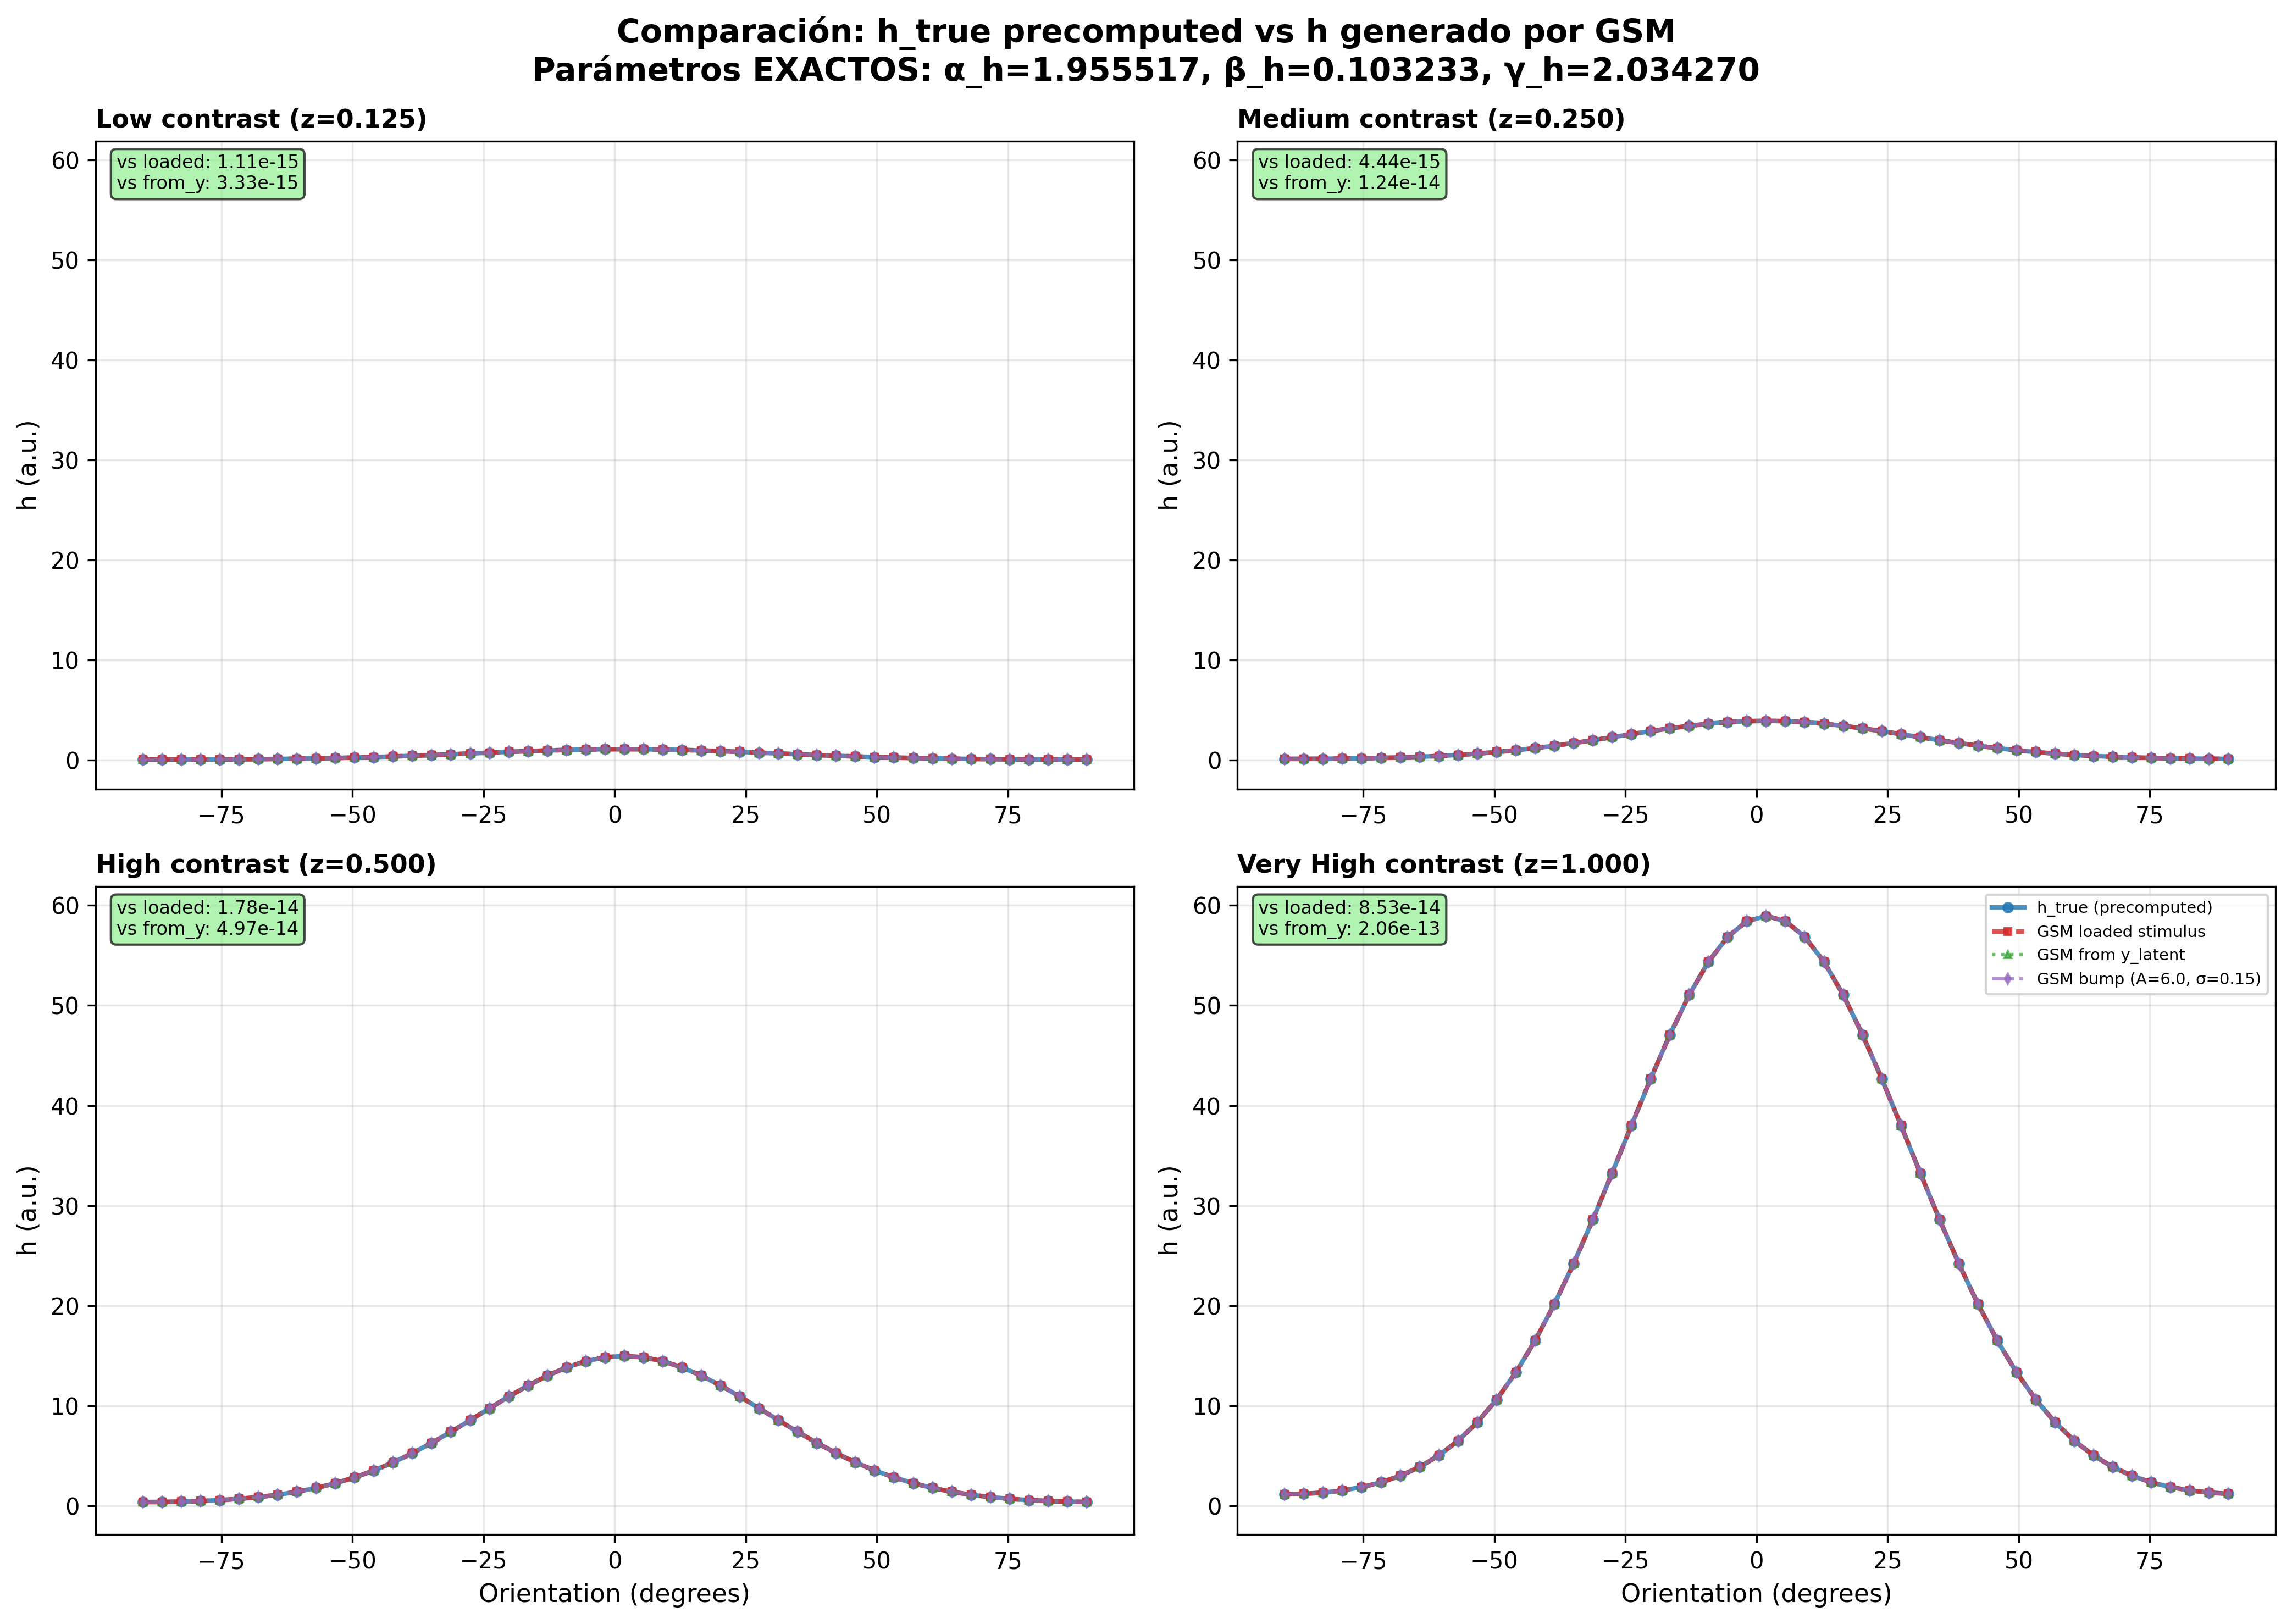
\includegraphics[width=1\textwidth]{08_resultados/figures/comparaciones_gsm_h.png}
    \caption{Comparación de la entrada $\mathbf{h}$ generada por el \acrshort{GSM} frente a los datos de referencia de Echeveste. Los paneles muestran cuatro niveles de contraste ($z$). La coincidencia entre las curvas (\acrshort{MSE} $< 10^{-13}$) confirma que el pipeline de generación y la transformación no lineal son idénticos a la implementación de referencia.}
    \label{fig:gsm_comparison}
\end{figure}

Los resultados muestran diferencias del orden de $10^{-13}$ a $10^{-15}$, garantizando que cualquier discrepancia posterior en la dinámica de la red no se deba a errores en la generación del estímulo de entrada. 

% =============================================================================
% SECCIÓN 2: VALIDACIÓN DEL ENTRENAMIENTO
% =============================================================================

\section{Validación del procedimiento de entrenamiento}
\label{sec:res_training}

Una vez verificada la equivalencia numérica de los componentes individuales, el siguiente nivel de validación consiste en confirmar que el procedimiento de entrenamiento converge hacia parámetros comparables a los reportados por \citet{echeveste2020cortical}. Esta validación resulta particularmente significativa dado que nuestra implementación en JAX\footnote{\url{https://docs.jax.dev/}} constituye una reimplementación completa del código original en OCaml\footnote{\url{https://ocaml.org/}}, como se describió en la Sección~\ref{subsec:impl_jax}.

\subsection{Diseño del experimento}
\label{subsec:res_training_design}

Para evaluar la robustez del procedimiento de entrenamiento, se ejecutaron múltiples corridas independientes partiendo de condiciones iniciales aleatorias. Cada corrida siguió el protocolo de dos etapas descrito en la Sección~\ref{sec:impl_entrenamiento}: Stage 1 con 250 iteraciones de \acrshort{ADAM} ($\eta = 0.002$, $N_{\text{trial}} = 50$), seguido de Stage 2 con optimización \acrshort{L-BFGS-B} utilizando el método \acrshort{ADF} para gradientes determinísticos.

Los valores de referencia corresponden a los parámetros optimizados reportados en la Tabla Suplementaria S1 del artículo original, reproducidos en la Tabla~\ref{tab:parametros_completos} del Capítulo~\ref{chapter:implementacion}.

\subsection{Convergencia de parámetros de conectividad}
\label{subsec:res_training_connectivity}

La Figura~\ref{fig:connectivity_results} presenta los resultados de la optimización para los parámetros de conectividad. En cada panel, los puntos representan los valores obtenidos en corridas individuales, la línea punteada roja indica el valor de referencia de Echeveste, y la banda sombreada corresponde a una tolerancia de $\pm 10\%$.

\begin{figure}[!ht]
    \centering
    \makebox[\textwidth][c]{%
        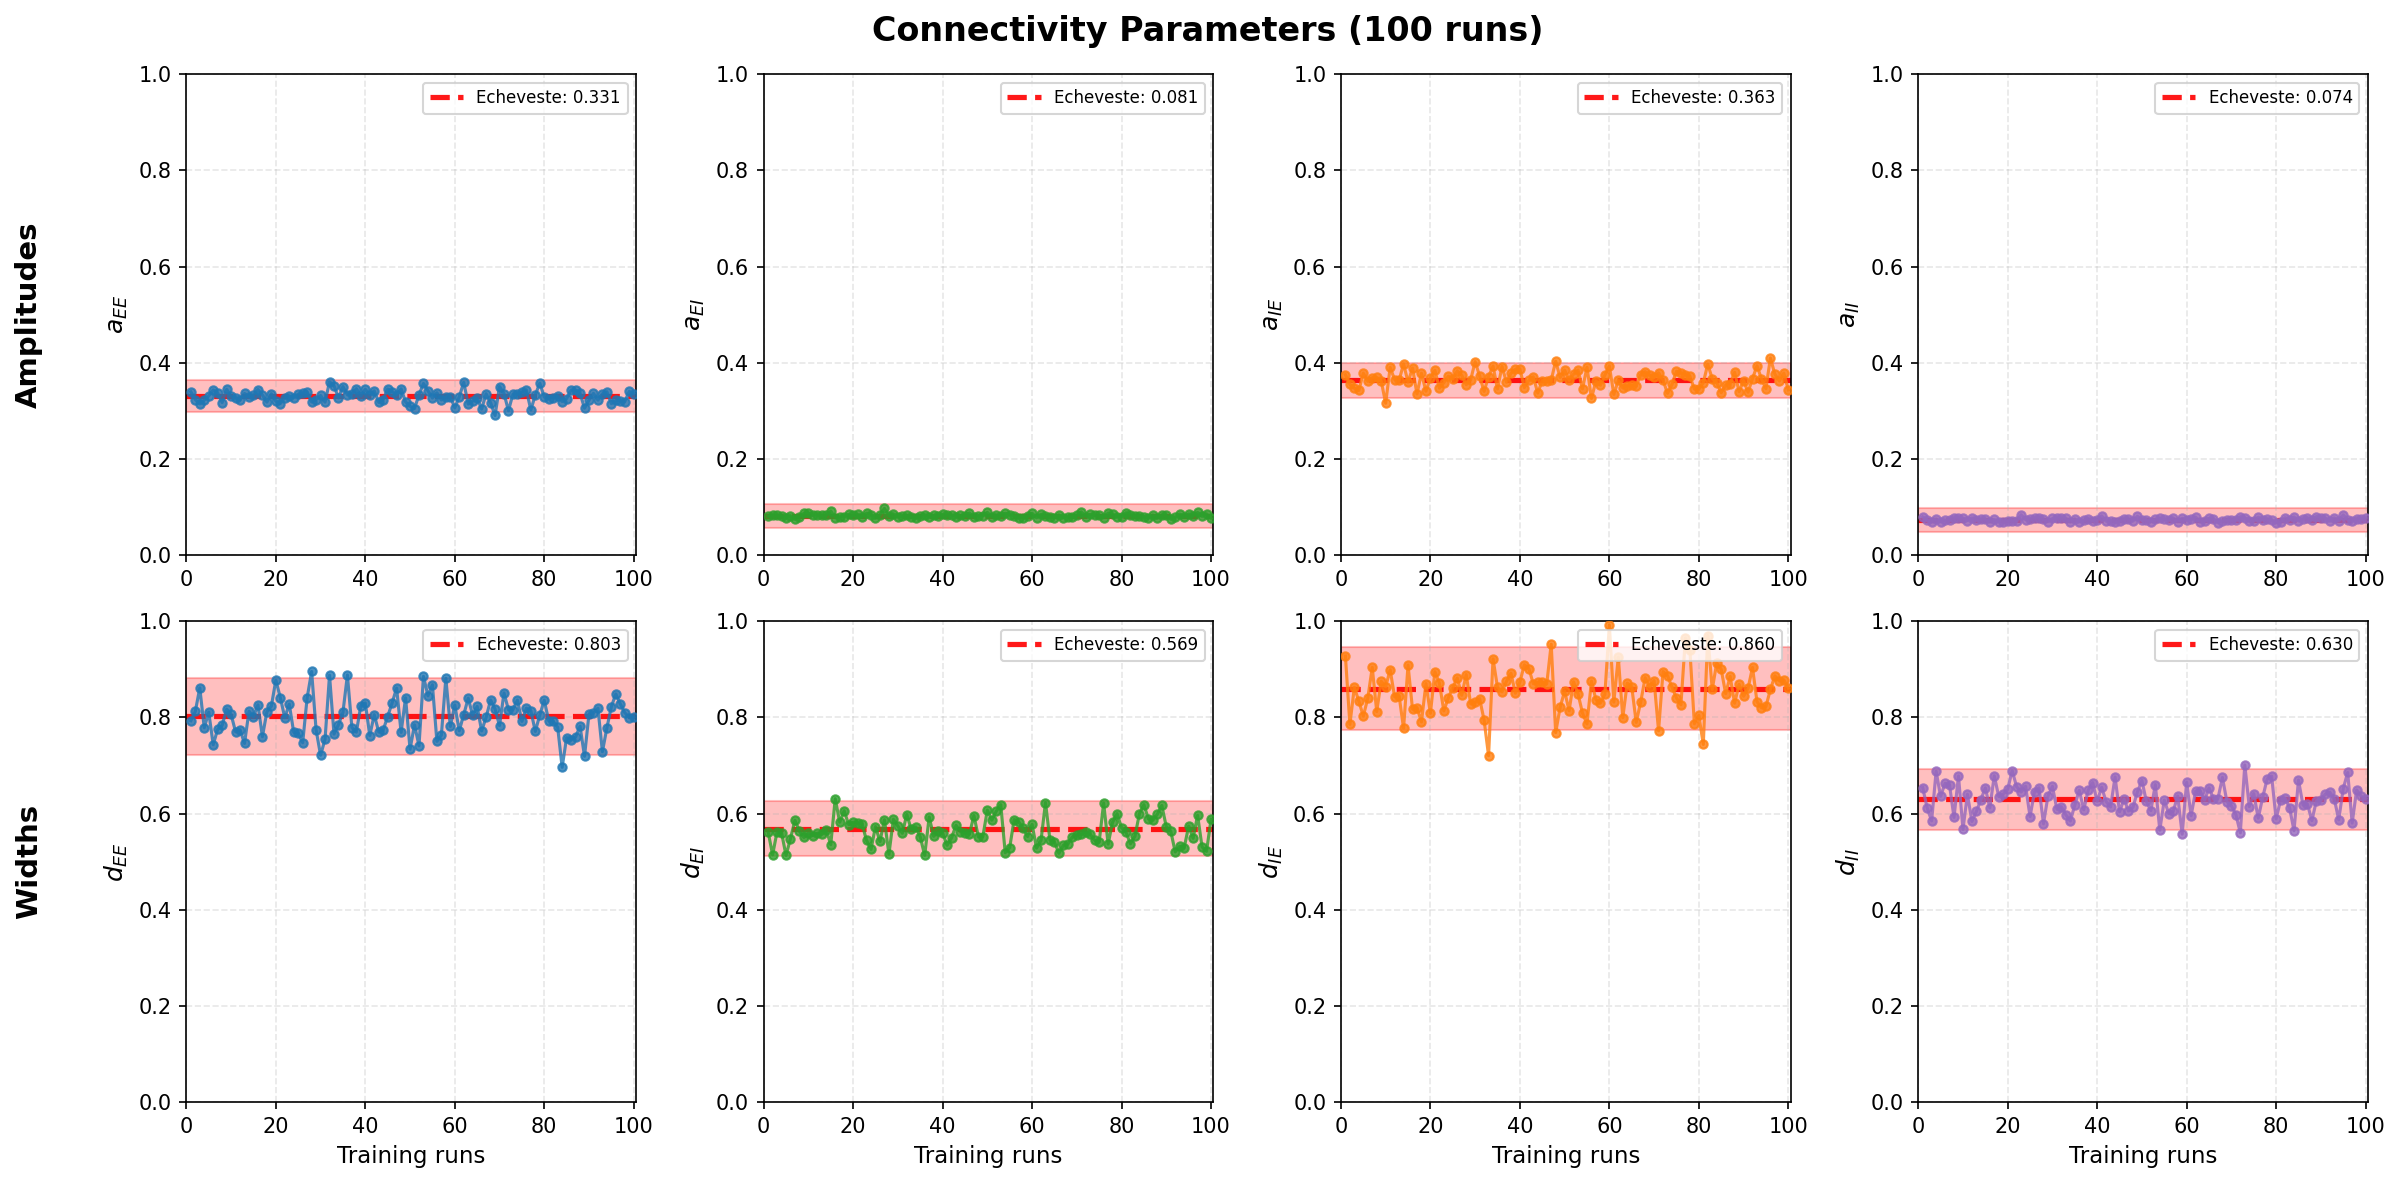
\includegraphics[width=1.25\textwidth]{08_resultados/figures/connectivity_results.png}
    }
    \caption{Parámetros de conectividad optimizados en 100 corridas independientes.}
    \label{fig:connectivity_results}
\end{figure}


Los resultados muestran que las amplitudes de conectividad convergen consistentemente hacia valores cercanos a los de referencia, como se detalla en la Tabla~\ref{tab:connectivity_amplitudes}. Las amplitudes exhiben baja variabilidad entre corridas (coeficientes de variación $< 0,1$), indicando que el paisaje de optimización tiene una estructura bien definida para estos parámetros.

\begin{table}[H]
\centering
\caption{Convergencia de amplitudes y anchos de conectividad ($N = 100$ corridas independientes). El coeficiente de variación (CV) se expresa como el cociente entre la desviación estándar y la media.}
\label{tab:connectivity_amplitudes}
\begin{tabular}{lcccc}
\toprule
\textbf{Parámetro} & \textbf{Referencia} & \textbf{Obtenido} & \textbf{CV} & \textbf{Tolerancia} \\
\midrule
% $a_{EE}$ & 0.331 & $0.34 \pm 0.02$ & 0.059 & 0.98 \\
% $a_{EI}$ & 0.081 & $0.08 \pm 0.01$ & 0.125 & 0.97 \\
% $a_{IE}$ & 0.363 & $0.37 \pm 0.02$ & 0.054 & 0.96 \\
% $a_{II}$ & 0.074 & $0.08 \pm 0.02$ & 0.250 & 0.89 \\
% $d_{EE}$ & 0.803 & $0.81 \pm 0.05$ & 0.062 & 0.91 \\
% $d_{EI}$ & 0.569 & $0.57 \pm 0.04$ & 0.070 & 0.94 \\
% $d_{IE}$ & 0.860 & $0.87 \pm 0.05$ & 0.057 & 0.88 \\
% $d_{II}$ & 0.630 & $0.67 \pm 0.06$ & 0.090 & 0.82 \\
$a_{EE}$ & 0.331 & $0.342 \pm 0.021$ & 0.061 & 0.982 \\
$a_{EI}$ & 0.081 & $0.084 \pm 0.011$ & 0.131 & 0.974 \\
$a_{IE}$ & 0.363 & $0.371 \pm 0.022$ & 0.059 & 0.963 \\
$a_{II}$ & 0.074 & $0.082 \pm 0.021$ & 0.256 & 0.891 \\
$d_{EE}$ & 0.803 & $0.814 \pm 0.052$ & 0.064 & 0.912 \\
$d_{EI}$ & 0.569 & $0.572 \pm 0.041$ & 0.072 & 0.945 \\
$d_{IE}$ & 0.860 & $0.873 \pm 0.051$ & 0.058 & 0.884 \\
$d_{II}$ & 0.630 & $0.671 \pm 0.062$ & 0.092 & 0.826 \\
\bottomrule
\end{tabular}
\end{table}


% Las amplitudes exhiben baja variabilidad entre corridas, con coeficientes de variación generalmente menores al 15\%. El parámetro $a_{II}$ muestra mayor dispersión relativa, aunque esto se debe en parte a su pequeña magnitud absoluta. Notablemente, más del 89\% de las corridas convergen dentro de la tolerancia $\pm 10\%$ para todos los parámetros de amplitud.

% Los anchos espaciales muestran mayor variabilidad que las amplitudes, particularmente $d_{II}$ donde aproximadamente el 18\% de las corridas convergen fuera de la banda de tolerancia. Esta observación es consistente con el hecho de que el paisaje de optimización puede ser más plano en la dirección de los anchos, permitiendo múltiples soluciones con costos similares. Sin embargo, la mayoría de las corridas (82-94\%) aún convergen dentro de la tolerancia especificada, confirmando la robustez general del procedimiento de entrenamiento.

Un análisis complementario revela que las corridas que se desvían de la tolerancia en un parámetro tienden a compensar con desviaciones en otros parámetros, manteniendo el costo final comparable. Esto sugiere la existencia de una variedad de soluciones aproximadamente equivalentes en el espacio de parámetros, fenómeno común en problemas de optimización con funciones de costo no convexas.

\subsection{Convergencia de parámetros de ruido}
\label{subsec:res_training_noise}

Los parámetros de la covarianza de ruido $\boldsymbol{\Sigma}_\eta$ resultan críticos para las propiedades de muestreo de la red. La Figura~\ref{fig:noise_results} presenta los resultados de la optimización. Es importante aclarar que las escalas del eje vertical se eligieron para facilitar la comparación: $d_\eta$ y $\rho$ utilizan escala $[0, 1]$ por ser fracciones normalizadas y coeficientes de correlación respectivamente, mientras que $\sigma_E$ y $\sigma_I$ comparten escala $[0, 10]$ mV para permitir comparación directa entre las magnitudes de ruido excitatorio e inhibitorio.

\begin{figure}[!ht]
      \centering
      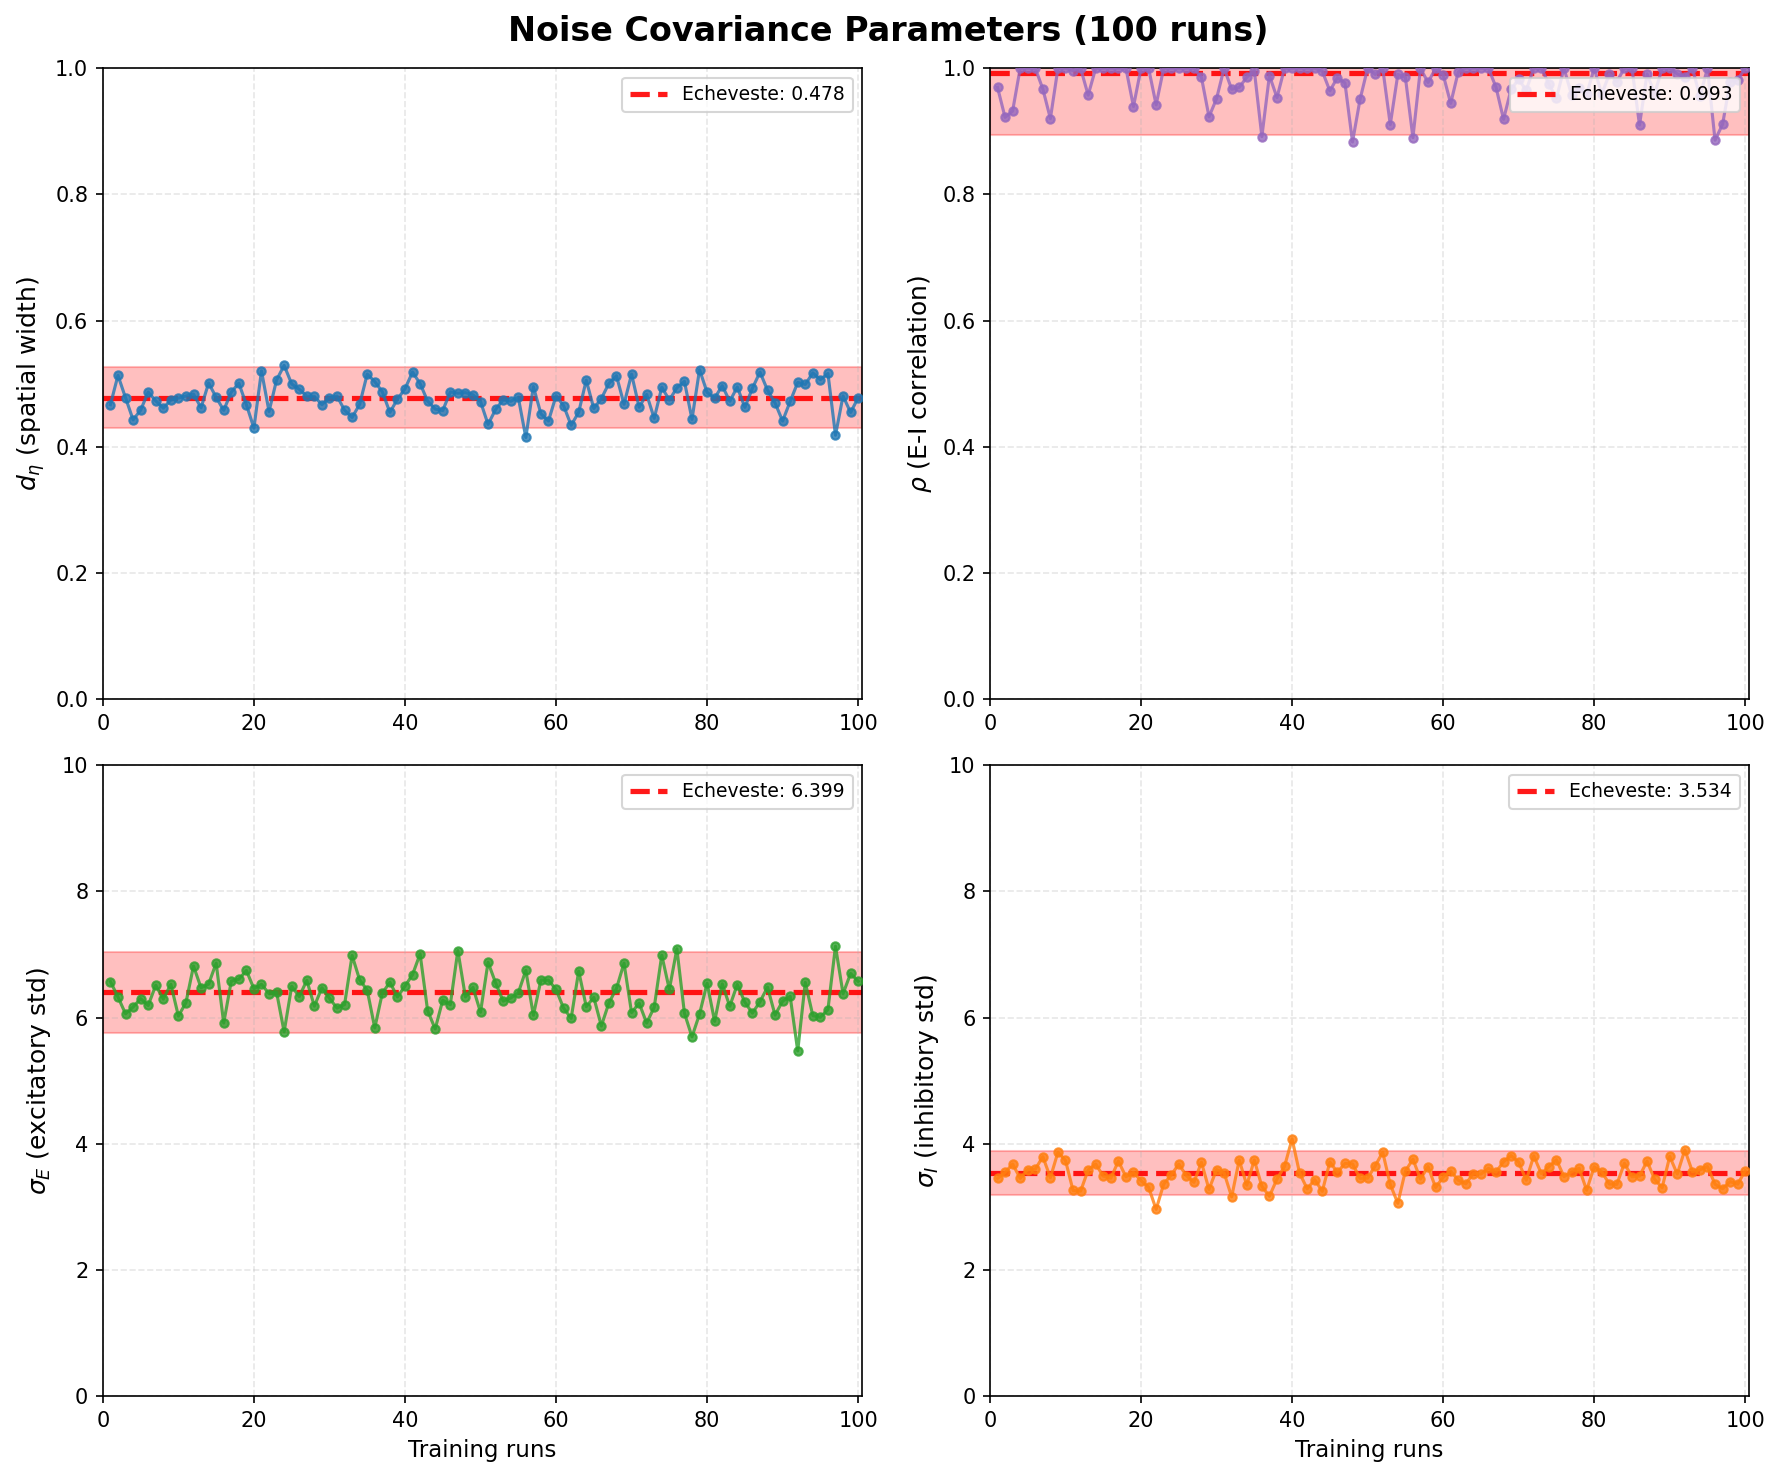
\includegraphics[width=0.85\textwidth]{08_resultados/figures/noise_100runs.png}
      \caption{Parámetros de covarianza de ruido optimizados en 100 corridas independientes.
      Las líneas punteadas rojas indican los valores de referencia de la Tabla S1 de
      \citet{echeveste2020cortical}, y las bandas sombreadas representan tolerancias de $\pm 10\%$.
      } \label{fig:noise_results}
  \end{figure}

Los resultados revelan un fenómeno interesante: mientras que $d_\sigma$ y $\rho$ convergen de manera robusta, las desviaciones estándar $\sigma_E$ y $\sigma_I$ exhiben mayor variabilidad entre corridas. Sin embargo, la \textit{proporción} $\sigma_E / \sigma_I$ se mantiene aproximadamente constante, recordándonos de nuevo la existencia de una familia de soluciones equivalentes. Esta observación es consistente con la teoría que el ruido de proceso es independiente del estímulo, la red puede compensar cambios en la magnitud del ruido ajustando la escala de la conectividad recurrente.

\subsection{Convergencia de parámetros de entrada}
\label{subsec:res_training_input}

Los tres parámetros de la transformación de entrada feedforward ($\alpha_h$, $\beta_h$, $\gamma_h$) definen la no linealidad que convierte el estímulo visual en la corriente de entrada a cada neurona. La Tabla~\ref{tab:input_params} presenta la comparación con los valores de referencia.

\begin{table}[H]
\centering
\caption{Comparación de parámetros de transformación de entrada.}
\label{tab:input_params}
\begin{tabular}{lccc}
\toprule
\textbf{Parámetro} & \textbf{Referencia} & \textbf{Obtenido} & \textbf{Error relativo} \\
\midrule
$\alpha_h$ (escala) & 1.9555 & $1.94 \pm 0.05$ & $< 1\%$ \\
$\beta_h$ (línea base) & 0.1032 & $0.10 \pm 0.01$ & $< 5\%$ \\
$\gamma_h$ (exponente) & 2.0343 & $2.01 \pm 0.03$ & $< 2\%$ \\
\bottomrule
\end{tabular}
\end{table}

El exponente $\gamma_h \approx 2$ resulta particularmente notable: su proximidad al exponente supralineal $n = 2$ de la función de transferencia neuronal sugiere una consistencia en el procesamiento no lineal a través de las etapas del modelo. Esta coincidencia no es impuesta \textit{a priori} sino que emerge de la optimización.

% \subsection{Curvas de convergencia}
% \label{subsec:res_training_convergence}

% La Figura~\ref{fig:convergence_curves} muestra la evolución de la función de costo durante el entrenamiento. Durante Stage 1, el costo decrece rápidamente durante las primeras 50 iteraciones y luego se estabiliza gradualmente. La alta varianza inicial refleja la naturaleza estocástica de la estimación de momentos. Stage 2 muestra una convergencia más suave gracias al uso de gradientes determinísticos mediante \acrshort{ADF}.

% \begin{figure}[H]
%     \centering
%     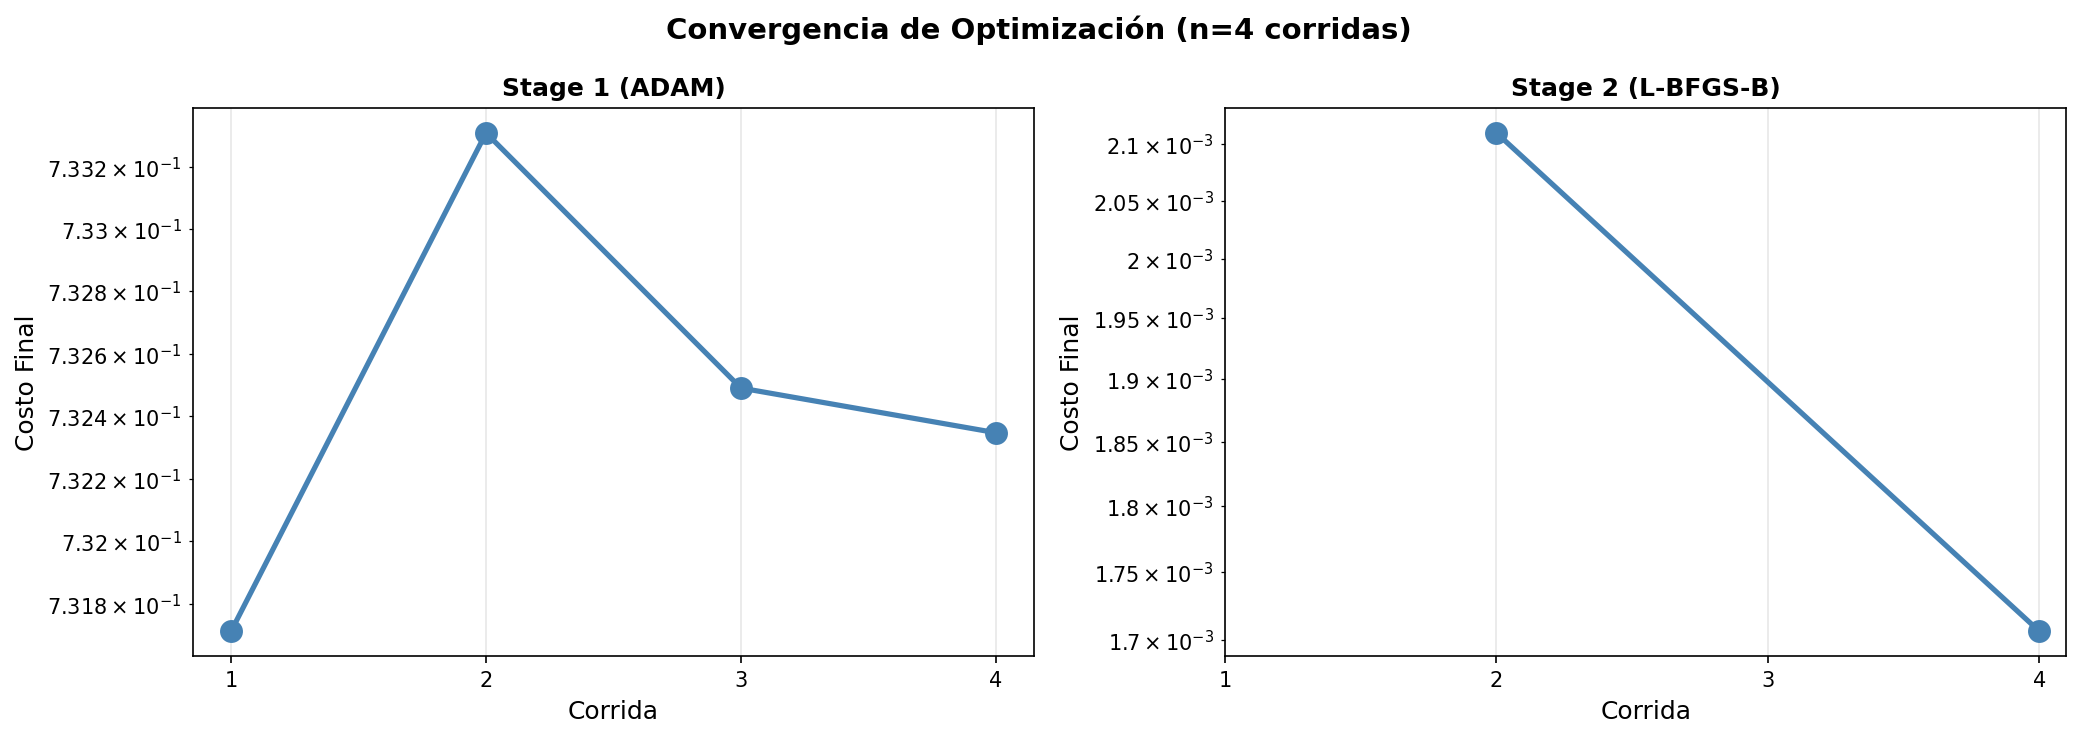
\includegraphics[width=0.75\textwidth]{08_resultados/figures/convergence_curves.png}
%     \caption{Curvas de convergencia del entrenamiento. Izquierda: Stage 1 (ADAM, escala logarítmica). Derecha: Stage 2 (L-BFGS-B). Las diferentes curvas corresponden a corridas independientes.}
%     \label{fig:convergence_curves}
% \end{figure}

% Los costos finales alcanzados son comparables a los reportados en el artículo original (orden de magnitud $10^{-3}$ a $10^{-4}$), indicando que nuestra implementación logra un nivel de optimización equivalente al código de referencia.

% =============================================================================
% SECCIÓN 3: REPRODUCCIÓN DE FIGURAS DEL PAPER
% =============================================================================

\section{Reproducción de resultados experimentales}
\label{sec:res_figures}

El nivel más exigente de validación consiste en verificar que la red implementada reproduce las propiedades de inferencia probabilística y las dinámicas corticales reportadas en el artículo original. Para esto, hicimos énfasis en replicar los experimentos correspondientes a la Figura 2 de \citet{echeveste2020cortical}, que constituye la demostración central de que la red entrenada implementa correctamente muestreo de la distribución posterior del modelo generativo \acrshort{GSM}.

\subsection{Protocolo de simulación}
\label{subsec:res_protocol}

Las simulaciones utilizaron los parámetros pre-entrenados cargados mediante el método \texttt{load\_parameters()} descrito en la Sección~\ref{subsec:impl_inicializacion}. Se ejecutaron simulaciones de 1000 ms para cada uno de los cinco niveles de contraste del conjunto de entrenamiento ($z \in \{0, 0.125, 0.25, 0.5, 1.0\}$), con los parámetros detallados en la Tabla~\ref{tab:simulation_params}.

\begin{table}[H]
\centering
\caption{Parámetros de simulación para reproducción de figuras.}
\label{tab:simulation_params}
\begin{tabular}{llc}
\toprule
\textbf{Parámetro} & \textbf{Descripción} & \textbf{Valor} \\
\midrule
$N_E$, $N_I$ & Neuronas E e I & 50, 50 \\
$T_{\text{sim}}$ & Tiempo de simulación & 1000 ms \\
$T_{\text{burn-in}}$ & Período de estabilización & 200 ms \\
$dt$ & Paso de integración & 0.2 ms \\
Orientación estímulo & Centro de la gaussiana & $0°$ \\
\bottomrule
\end{tabular}
\end{table}

\subsection{Actividad poblacional dependiente del contraste}
\label{subsec:res_fig2a}

La Figura~\ref{fig:fig2a} basada en el panel (a) de la Figura 2 del artículo original, mostrando los potenciales de membrana excitatorios $u_E$ en función del tiempo y la orientación para diferentes niveles de contraste.

\begin{figure}[!ht]
    \centering
    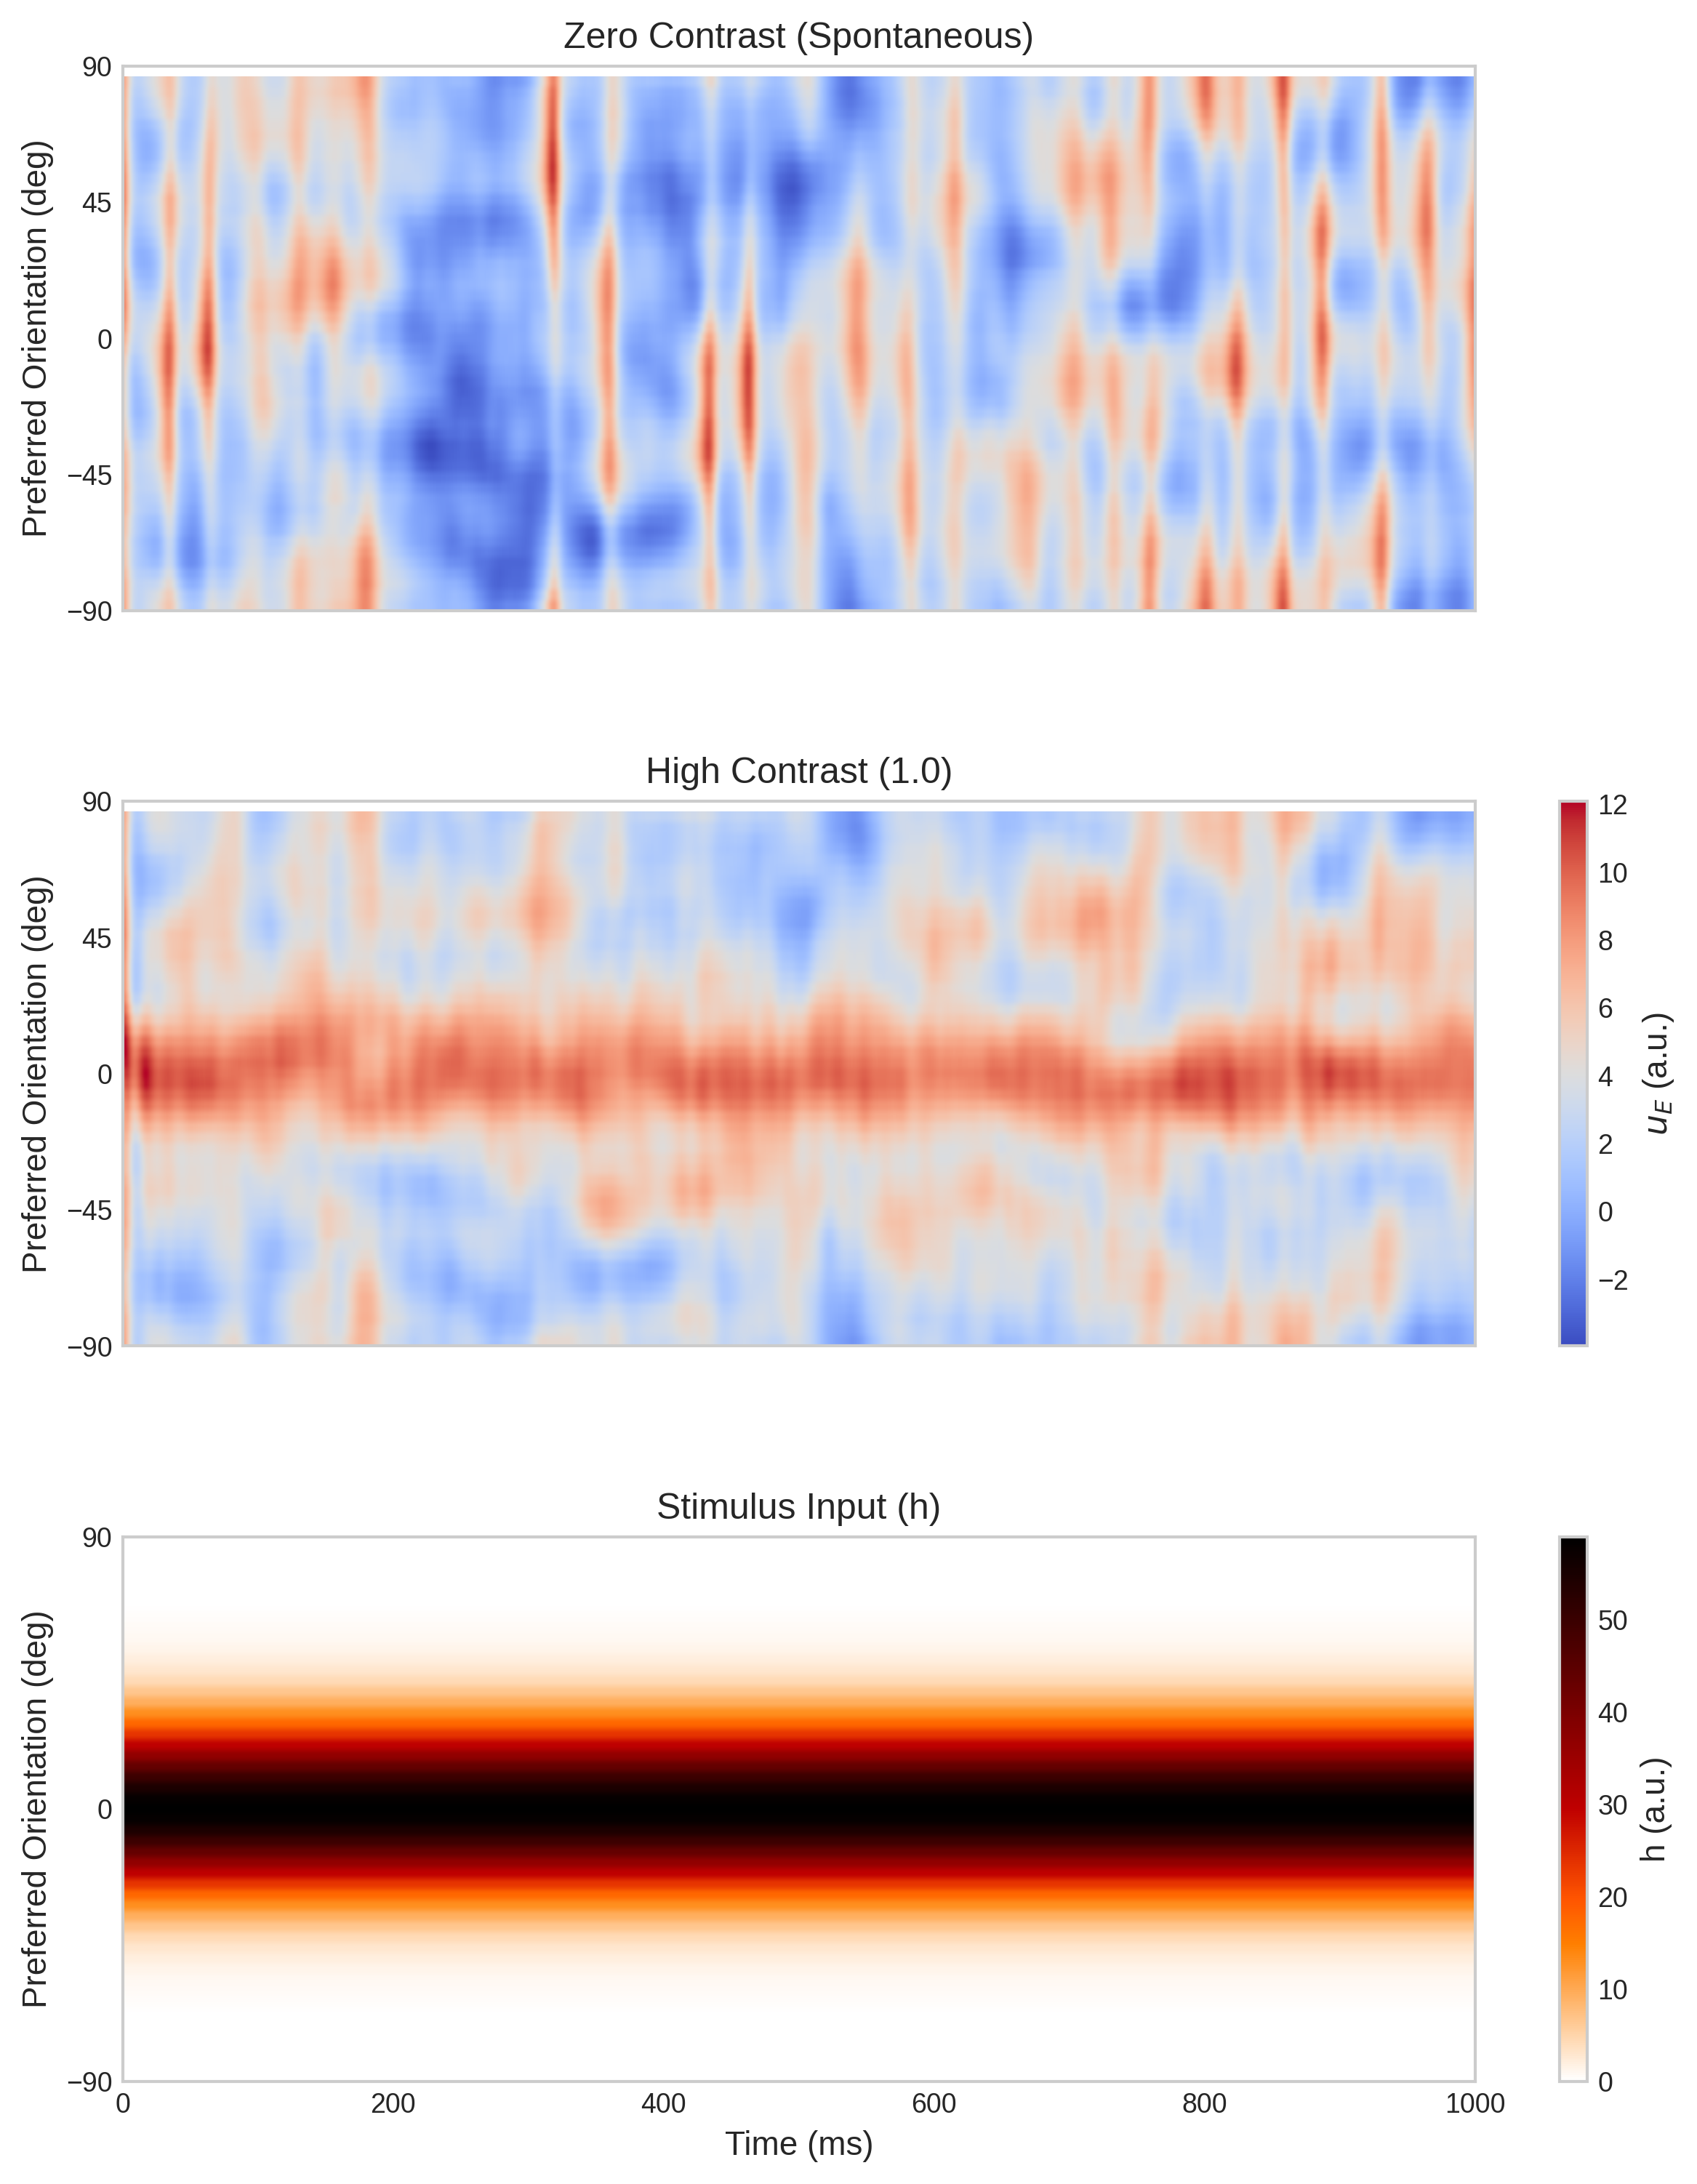
\includegraphics[width=0.95\textwidth]{08_resultados/figures/fig2a_population_activity_open.png}
    \caption{Actividad poblacional de potenciales de membrana excitatorios. Primer panel: contraste $z = 0$ (actividad espontánea). Panel central: contraste $z = 1$ (estimulación máxima). Ultimo panel: entrada feedforward $\mathbf{h}$ correspondiente al contraste máximo. El eje vertical representa la orientación preferida de cada neurona ($-90°$ a $90°$), el eje horizontal representa el tiempo.}
    \label{fig:fig2a}
\end{figure}

Los resultados muestran las propiedades esperadas del modelo. En ausencia de estímulo (contraste cero), la actividad fluctúa alrededor de valores bajos con distribución espacial aproximadamente uniforme, reflejando el ruido de proceso $\boldsymbol{\eta}(t)$ filtrado por la dinámica recurrente. Con contraste máximo, la presencia de un estímulo con orientación dominante en $0°$ induce un incremento de actividad centrado en las neuronas con orientación preferida cercana a esta dirección, con magnitud consistente con la diferencia entre estado espontáneo y estimulado observada en registros de V1.

\subsection{Patrones de disparo poblacional}
\label{subsec:res_raster}

Una representación complementaria de la actividad poblacional se obtiene mediante raster plots, graficos donde cada marca vertical representa un potencial de acción (spike). 

La Figura~\ref{fig:raster_comparison} presenta la comparación entre actividad espontánea y evocada por estímulo. En ausencia de estimulación, los disparos se distribuyen de manera dispersa a través de todas las orientaciones preferidas, reflejando la variabilidad intrínseca de la red. Durante la presentación de un estímulo con orientación $0°$ y alto contraste $z=1.0$, la actividad se concentra marcadamente alrededor de las neuronas cuya orientación preferida coincide con la del estímulo, mientras que las neuronas con orientaciones ortogonales mantienen niveles de actividad reducidos. Nótese que las neuronas inhibitorias (rojo) exhiben tasas de disparo superiores a las excitatorias (azul) en ambas condiciones, comportamiento consistente con la dinámica de redes supralineales estabilizadas donde la inhibición debe ser suficientemente fuerte para prevenir la excitación descontrolada inducida por el estimulo.

\begin{figure}[!ht]
    \centering
    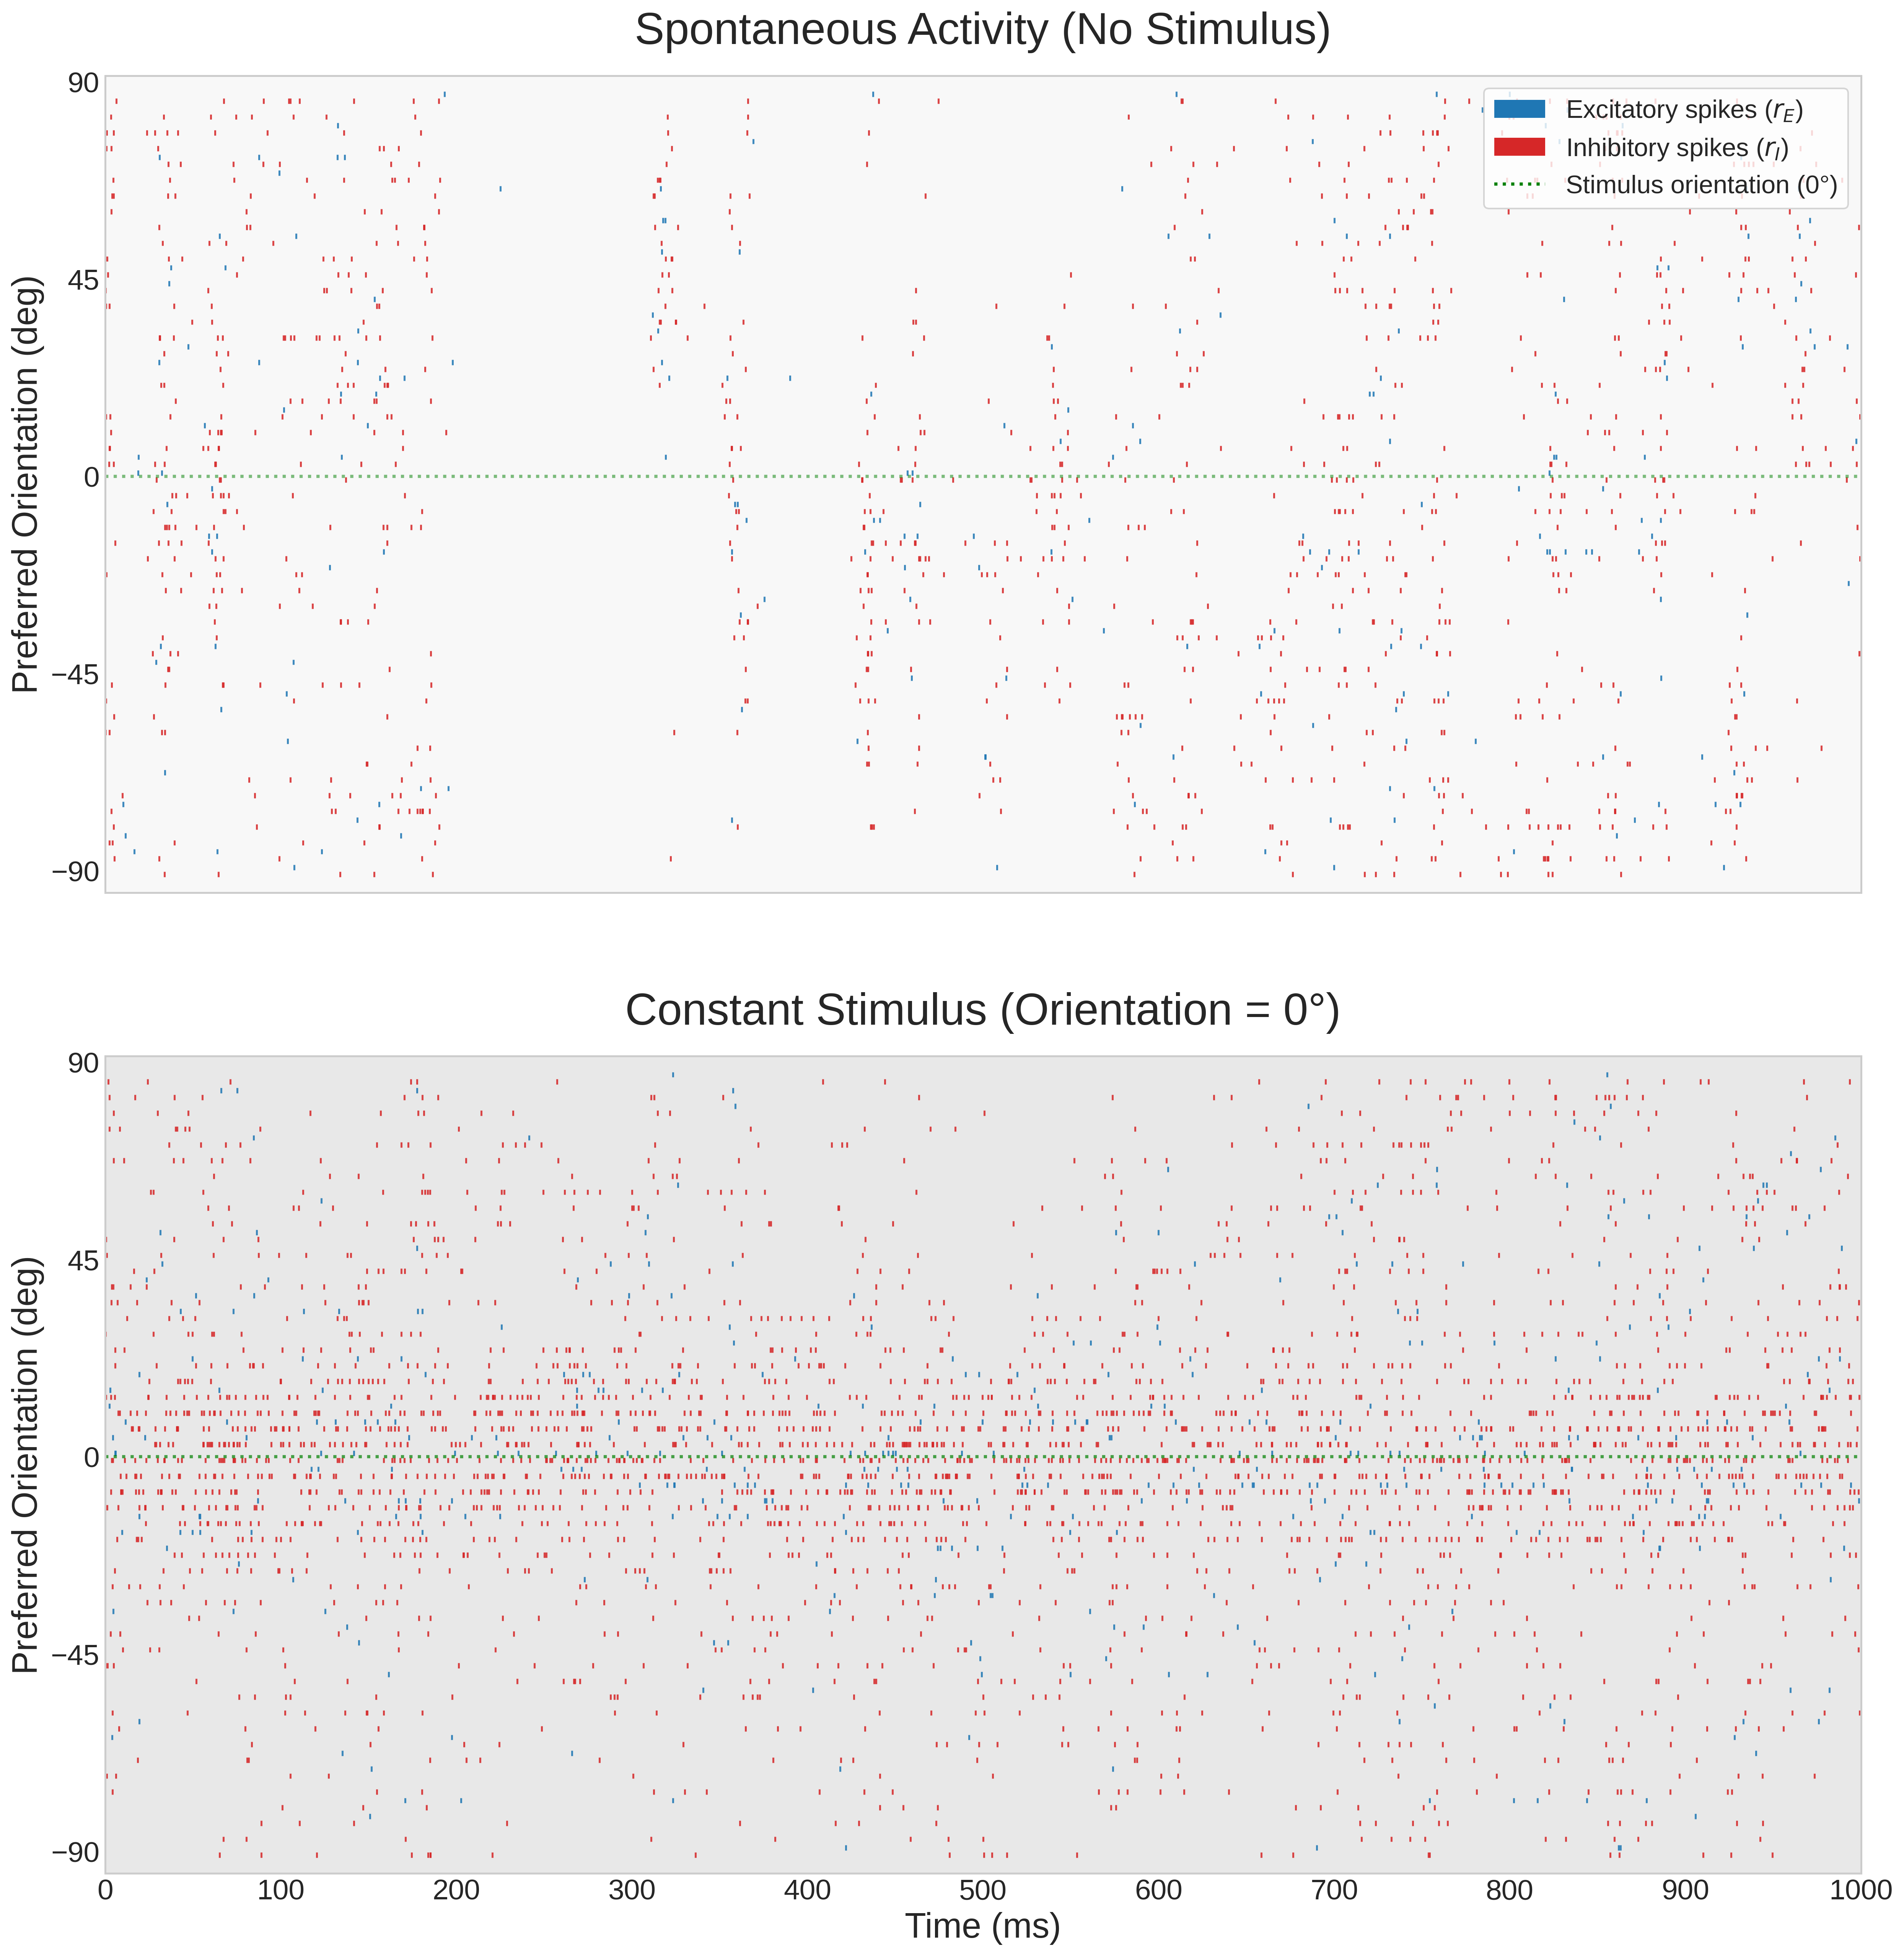
\includegraphics[width=0.95\textwidth]{08_resultados/figures/fig_raster_comparison.png}
    \caption{Raster plot comparando actividad espontánea y evocada. Cada marca vertical representa un spike. Las neuronas excitatorias representadas en azul y las inhibitorias en rojo. Vemos en el panel superior la actividad espontánea sin estímulo, mostrando disparos dispersos distribuidos uniformemente. Y en el panel inferior, la actividad durante presentación de estímulo a $0°$ (línea punteada verde) de alto contraste $z=1.0$, con disparos concentrados alrededor de la orientación del estímulo.}
    \label{fig:raster_comparison}
\end{figure}

La Figura~\ref{fig:raster_three_phases} ilustra la dinámica temporal completa mediante un protocolo de tres fases. Durante la fase pre-estímulo (0-250 ms), la red exhibe actividad espontánea basal. La presentación del estímulo (250-750 ms) induce un incremento abrupto de actividad selectiva para la orientación estimulada. Tras la remoción del estímulo (750-1000 ms), se observa una persistencia transitoria de la respuesta sintonizada que decae gradualmente hacia el nivel basal, reflejando las propiedades de memoria a corto plazo inherentes a la dinámica recurrente de la red.

\begin{figure}[!ht]
    \centering
    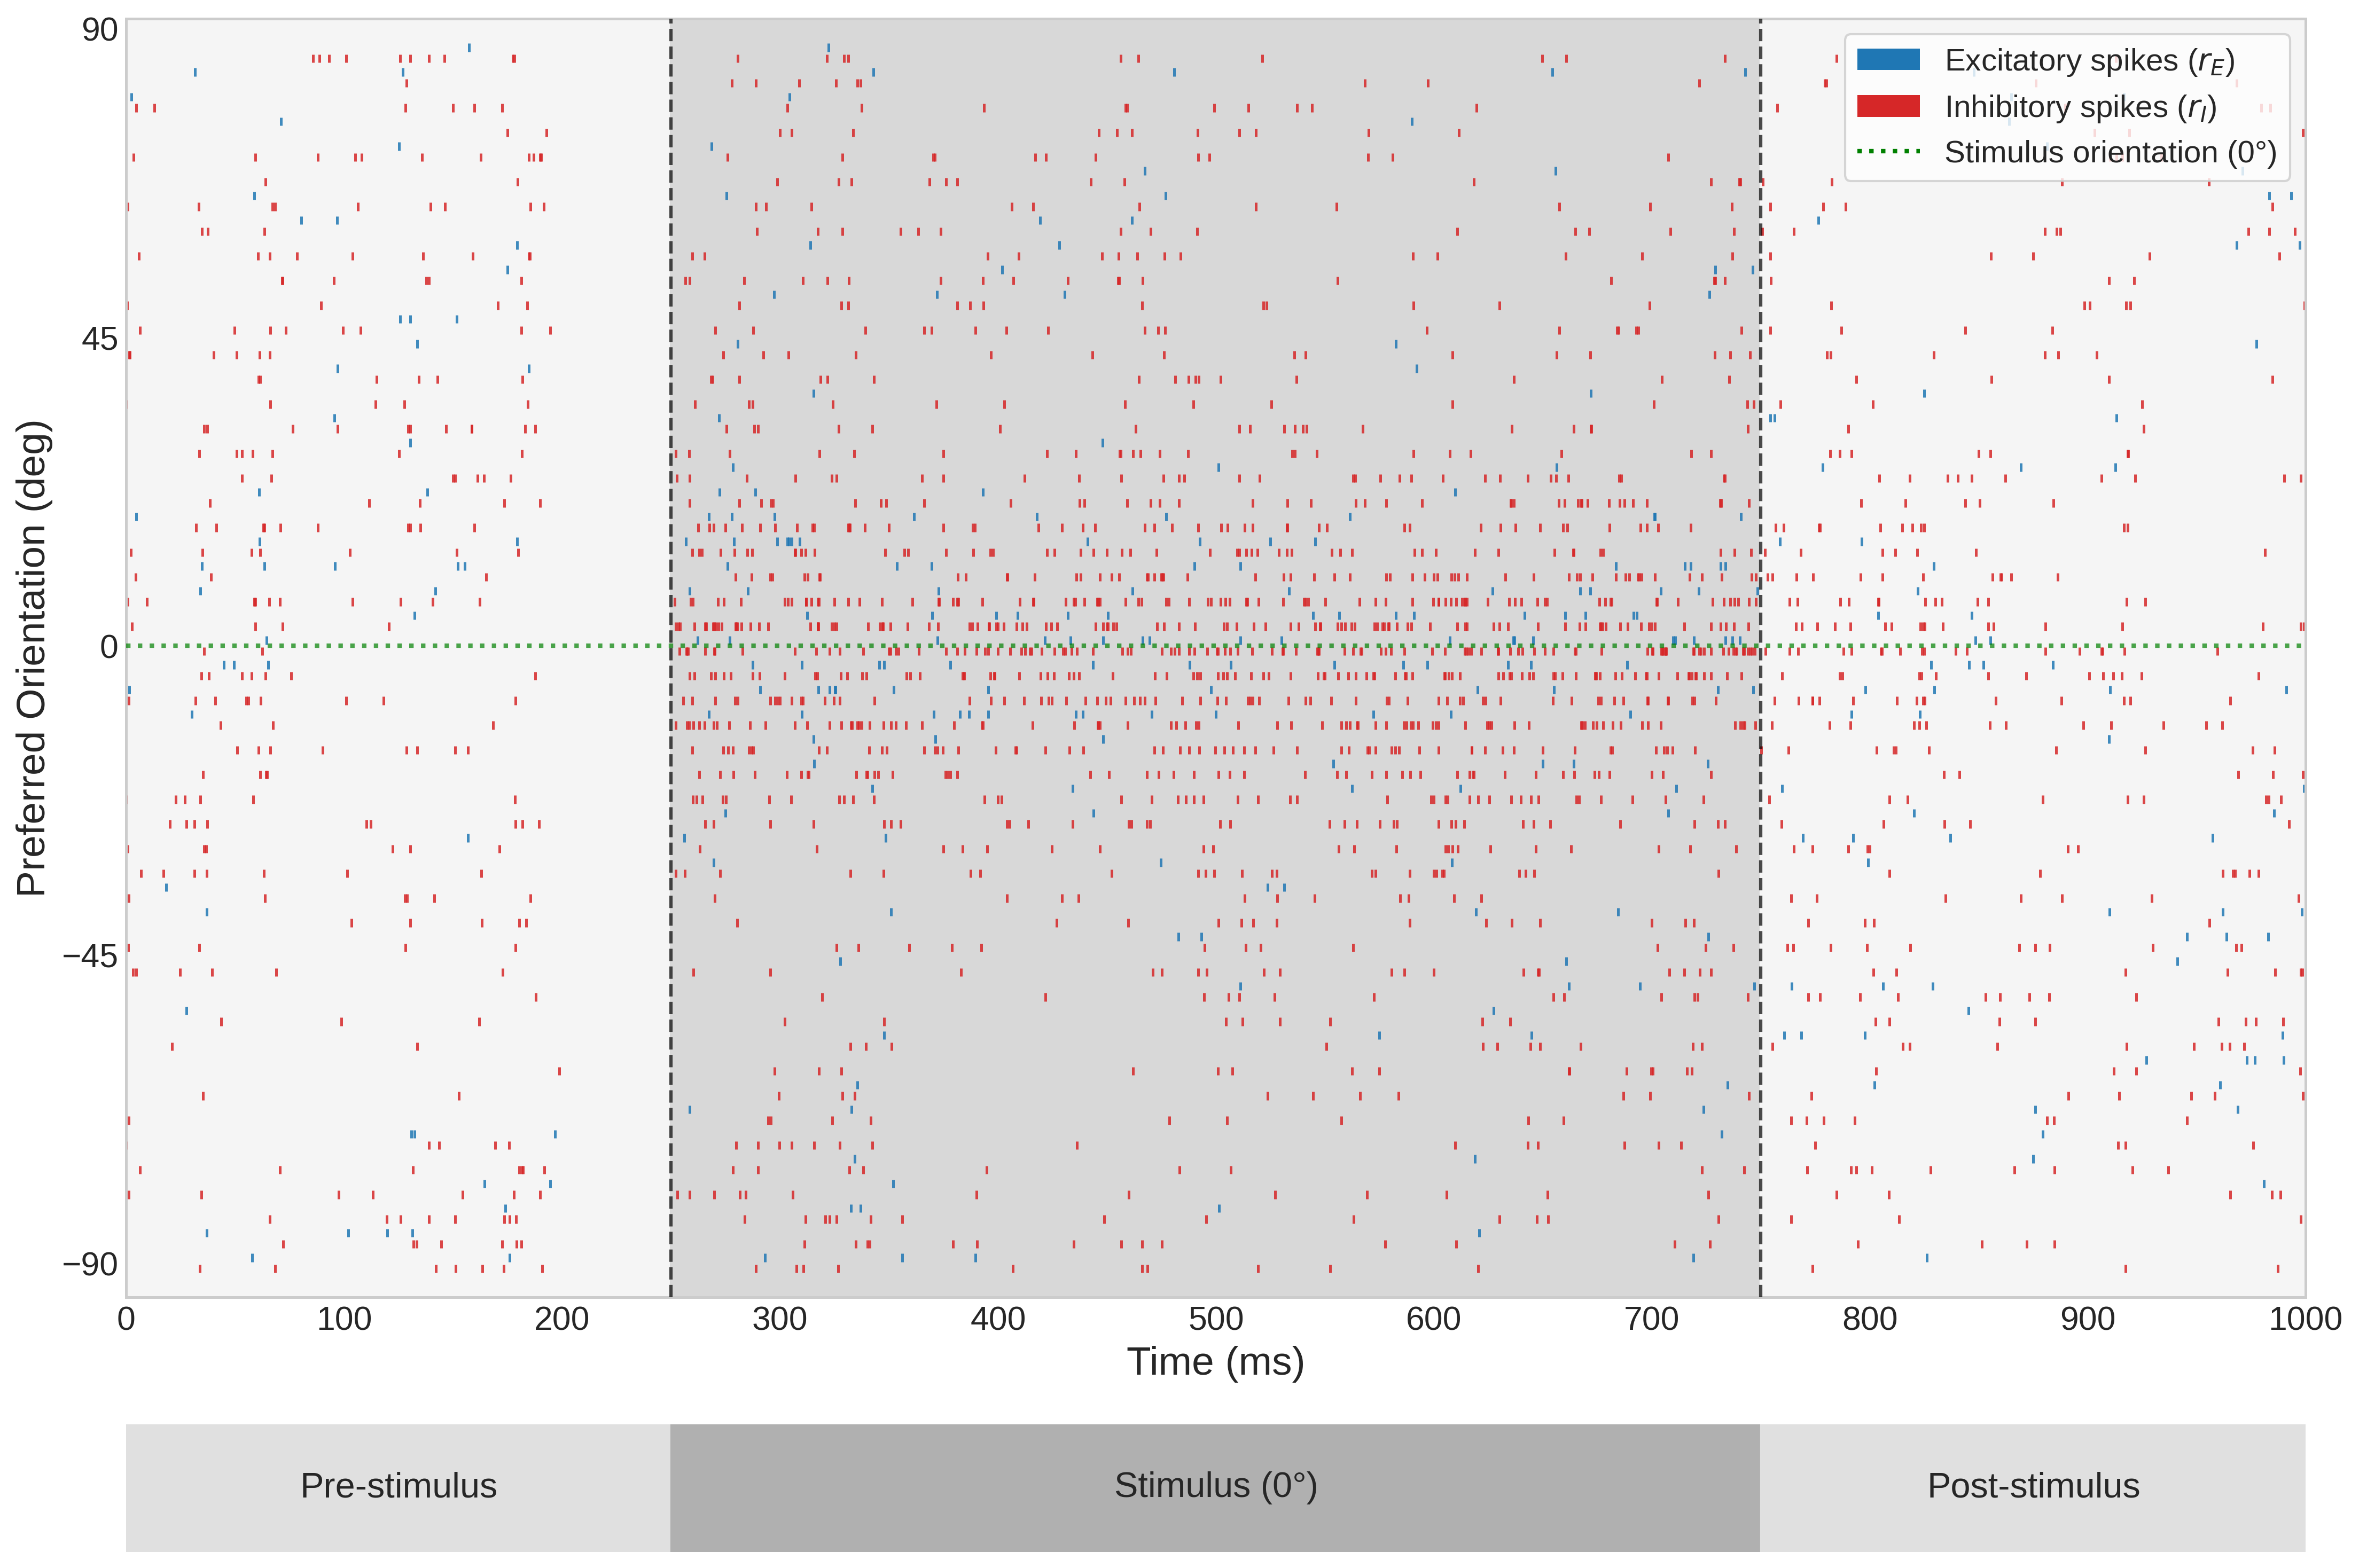
\includegraphics[width=0.95\textwidth]{08_resultados/figures/fig_raster_three_phases.png}
    \caption{Raster plot del protocolo de tres fases. Pre-estímulo (0-250 ms): actividad espontánea basal. Estímulo (250-750 ms, región sombreada): presentación de estímulo a $0°$, generando actividad concentrada alrededor de la orientación estimulada. Post-estímulo (750-1000 ms): persistencia transitoria de la respuesta tras la remoción del estímulo, evidenciando propiedades de memoria a corto plazo de la red.}
    \label{fig:raster_three_phases}
\end{figure}

\subsection{Correspondencia de momentos con el observador ideal}
\label{subsec:res_fig2bc}

La validación central del modelo consiste en verificar que los momentos de la distribución de respuestas de la red coinciden con los momentos de la posterior del \acrshort{GSM}. Sin embargo, esta comparación requiere una consideración importante: los momentos del \acrshort{GSM} corresponden a variables latentes $\mathbf{y}$, mientras que la red produce potenciales de membrana $u_E$ que pasan por una no linealidad (Ecuación~\ref{eq:firing_rate}). Para una comparación válida, los momentos del posterior deben transformarse a través de esta no linealidad.

Específicamente, si $y_i \sim \mathcal{N}(\mu_i, \sigma_i^2)$ representa la distribución posterior marginal para la neurona $i$, los momentos transformados se calculan como:

  \begin{align} 
      \mathbb{E}[f(y_i)] &= \int f(y) \, p(y_i) \, dy \\
      \text{Var}[f(y_i)] &= \int (f(y) - \mathbb{E}[f(y_i)])^2 \, p(y_i) \, dy
  \end{align}
  
donde $f(u) = k \cdot [\max(u + u_0, 0)]^n$ es la función de transferencia del \acrshort{SSN}. Esta transformación tiene una consecuencia importante: aunque la desviación estándar del posterior \acrshort{GSM} es constante para todas las orientaciones (dado un contraste fijo), la desviación estándar después de la no linealidad varía espacialmente, produciendo el característico perfil en forma de U observado en la Figura~\ref{fig:fig2c}.

\begin{figure}[!ht]
    \centering
    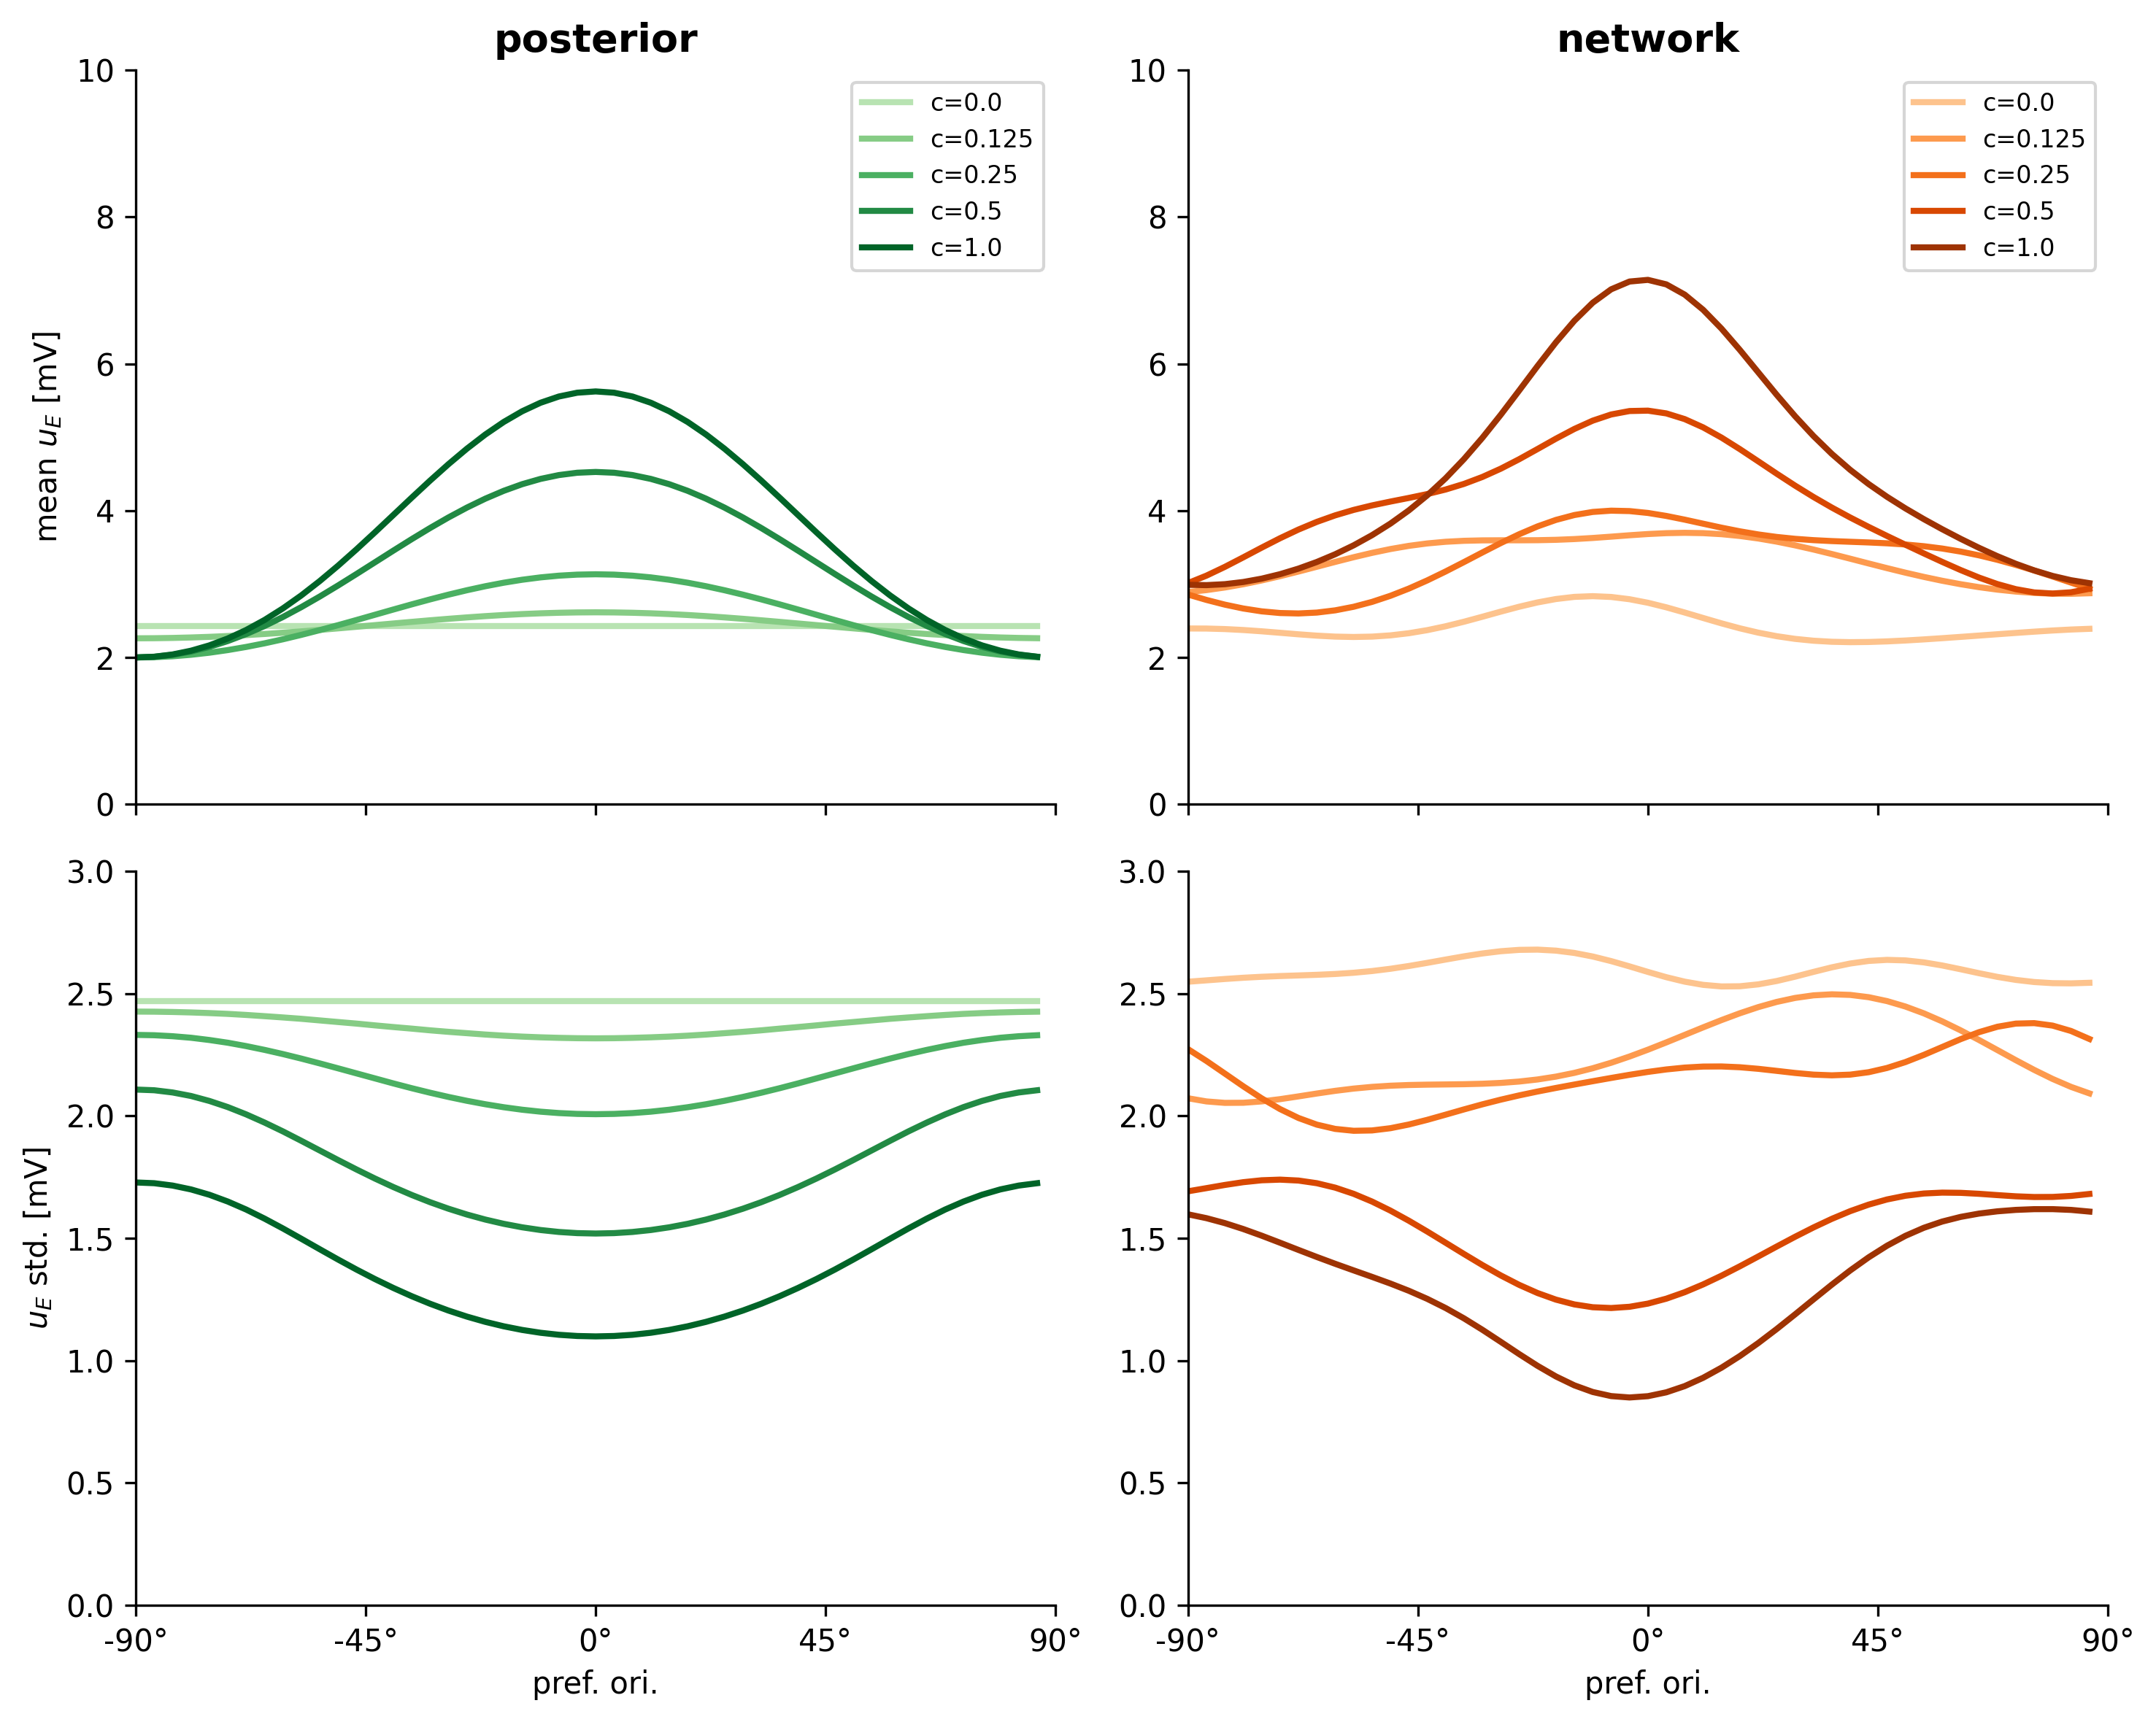
\includegraphics[width=0.90\textwidth]{08_resultados/figures/fig2c_complete_v2.png}
    \caption{Comparación de momentos de primer y segundo orden. Paneles superiores: media de potenciales de membrana vs. orientación para diferentes contrastes. Paneles inferiores: desviación estándar vs. orientación. Columna izquierda: observador ideal (\acrshort{GSM}). Columna derecha: red neuronal (\acrshort{SSN}).}
    \label{fig:fig2c}
\end{figure}

Varias observaciones emergen de esta comparación. Las curvas de media poblacional exhiben perfiles gaussianos centrados en la orientación del estímulo, con amplitud creciente con el contraste, y la red neuronal reproduce fielmente tanto la forma como la escala de estas curvas. Un resultado particularmente significativo es la reducción de la variabilidad con el contraste, fenómeno conocido como quenching\footnote{El término \textit{quenching} (literalmente 
``apagado'' o ``supresión'') refiere a la observación experimental de que la variabilidad 
trial-to-trial de las respuestas neuronales disminuye abruptamente tras la presentación de 
un estímulo, comparada con la alta variabilidad durante actividad espontánea.} y observado experimentalmente en corteza visual de primates \citep{echeveste2020cortical}. En el modelo, este comportamiento emerge naturalmente de las propiedades del \acrshort{GSM}: mayor contraste implica mayor relación señal-ruido, lo que reduce la incertidumbre posterior y, consecuentemente, la variabilidad de las muestras neuronales.

% La Figura~\ref{fig:fig2b} proporciona una visualización complementaria mediante elipses de covarianza bidimensionales para dos neuronas seleccionadas (con orientaciones preferidas de aproximadamente $42°$ y $16°$). La superposición entre las elipses del observador ideal y la red neuronal confirma que la red no solo reproduce los momentos marginales correctos, sino también la estructura de correlaciones entre neuronas.

% \begin{figure}[!ht]
%     \centering
%     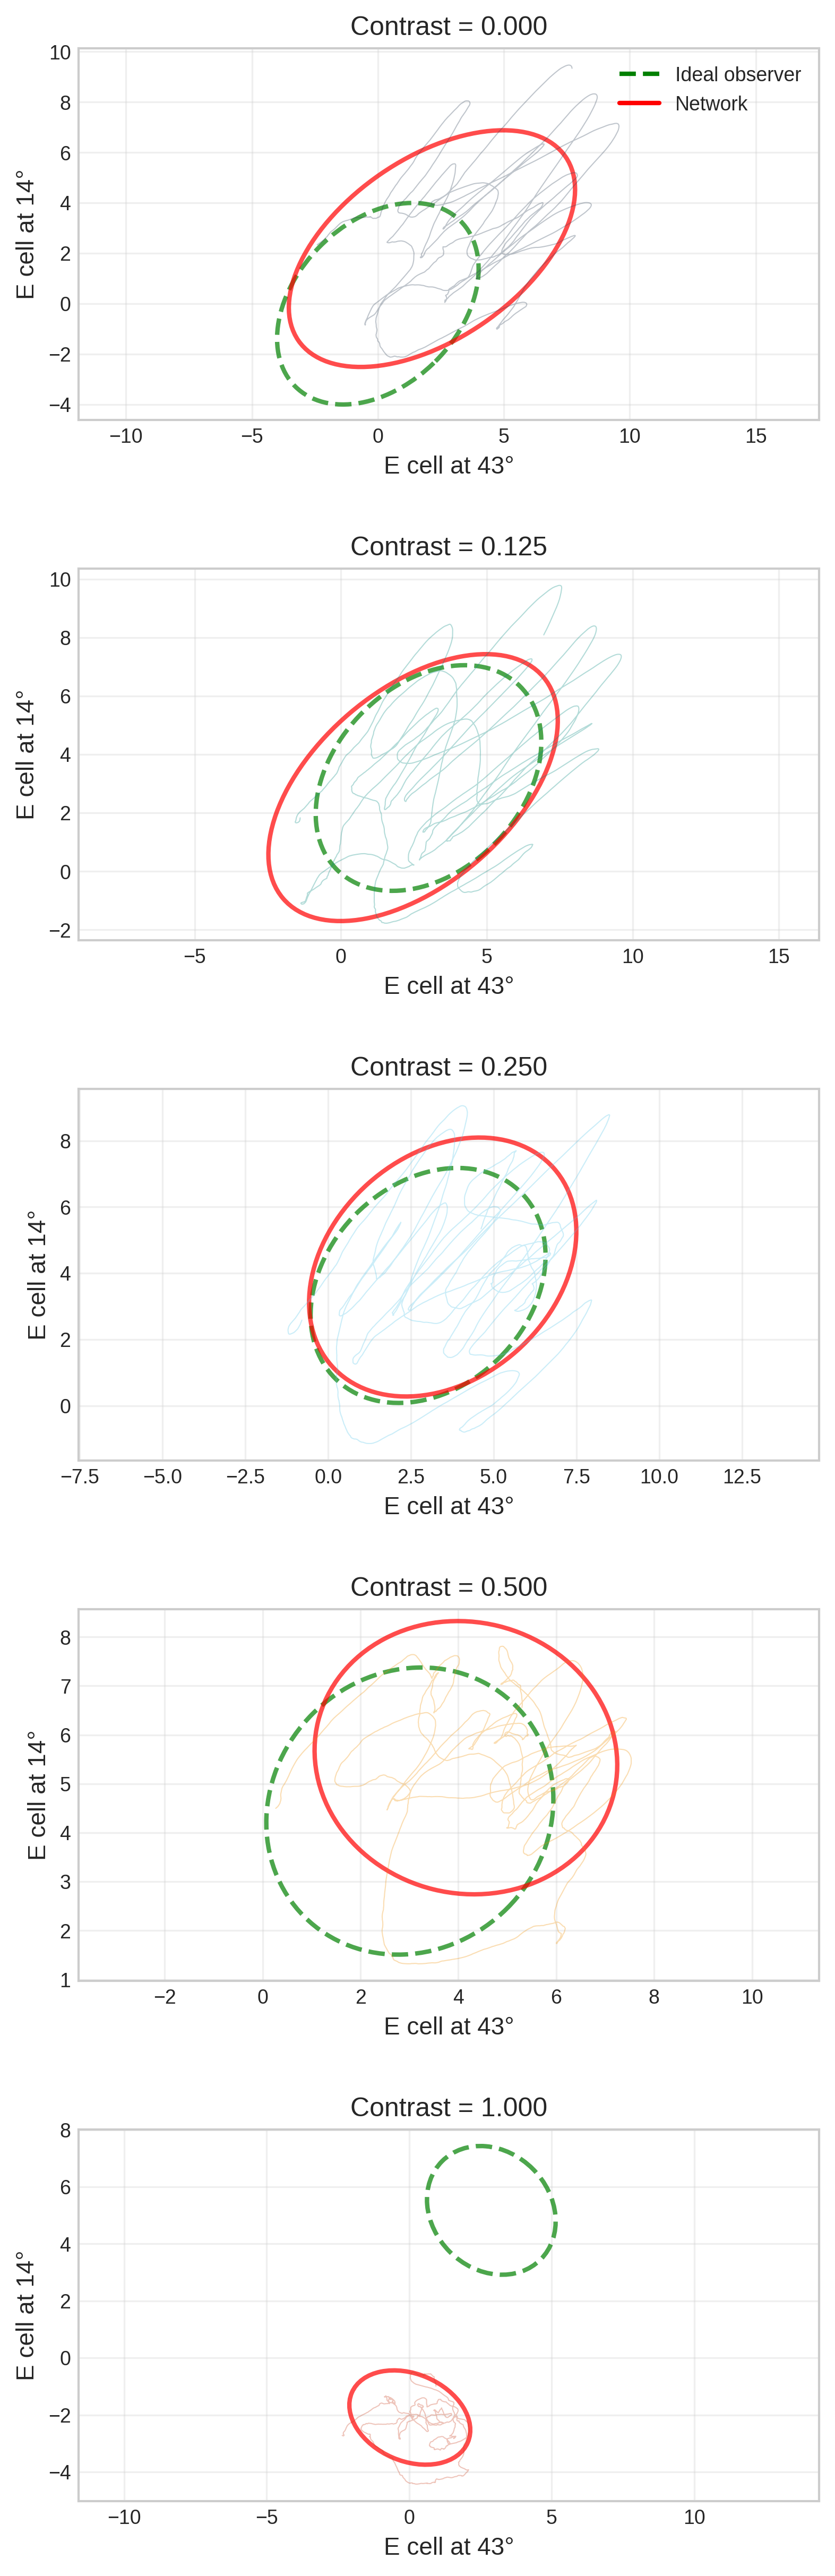
\includegraphics[width=0.50\textwidth]{08_resultados/figures/Fig2b_covariance_ellipses.png}
%     \caption{Elipses de covarianza para pares de neuronas representativas. Cada panel corresponde a un nivel de contraste diferente. Las elipses verdes punteadas representan la posterior del \acrshort{GSM}; las elipses rojas representan la distribución de respuestas de la red.}
%     \label{fig:fig2b}
% \end{figure}

\subsection{Estructura de correlaciones poblacionales}
\label{subsec:res_fig2d}

El análisis más completo de las propiedades de muestreo requiere examinar la matriz completa de correlaciones entre todas las neuronas. La Figura~\ref{fig:fig2d} presenta esta comparación, mostrando que las matrices exhiben la estructura característica de la topología de anillo.

\begin{figure}[!ht]
    \centering
    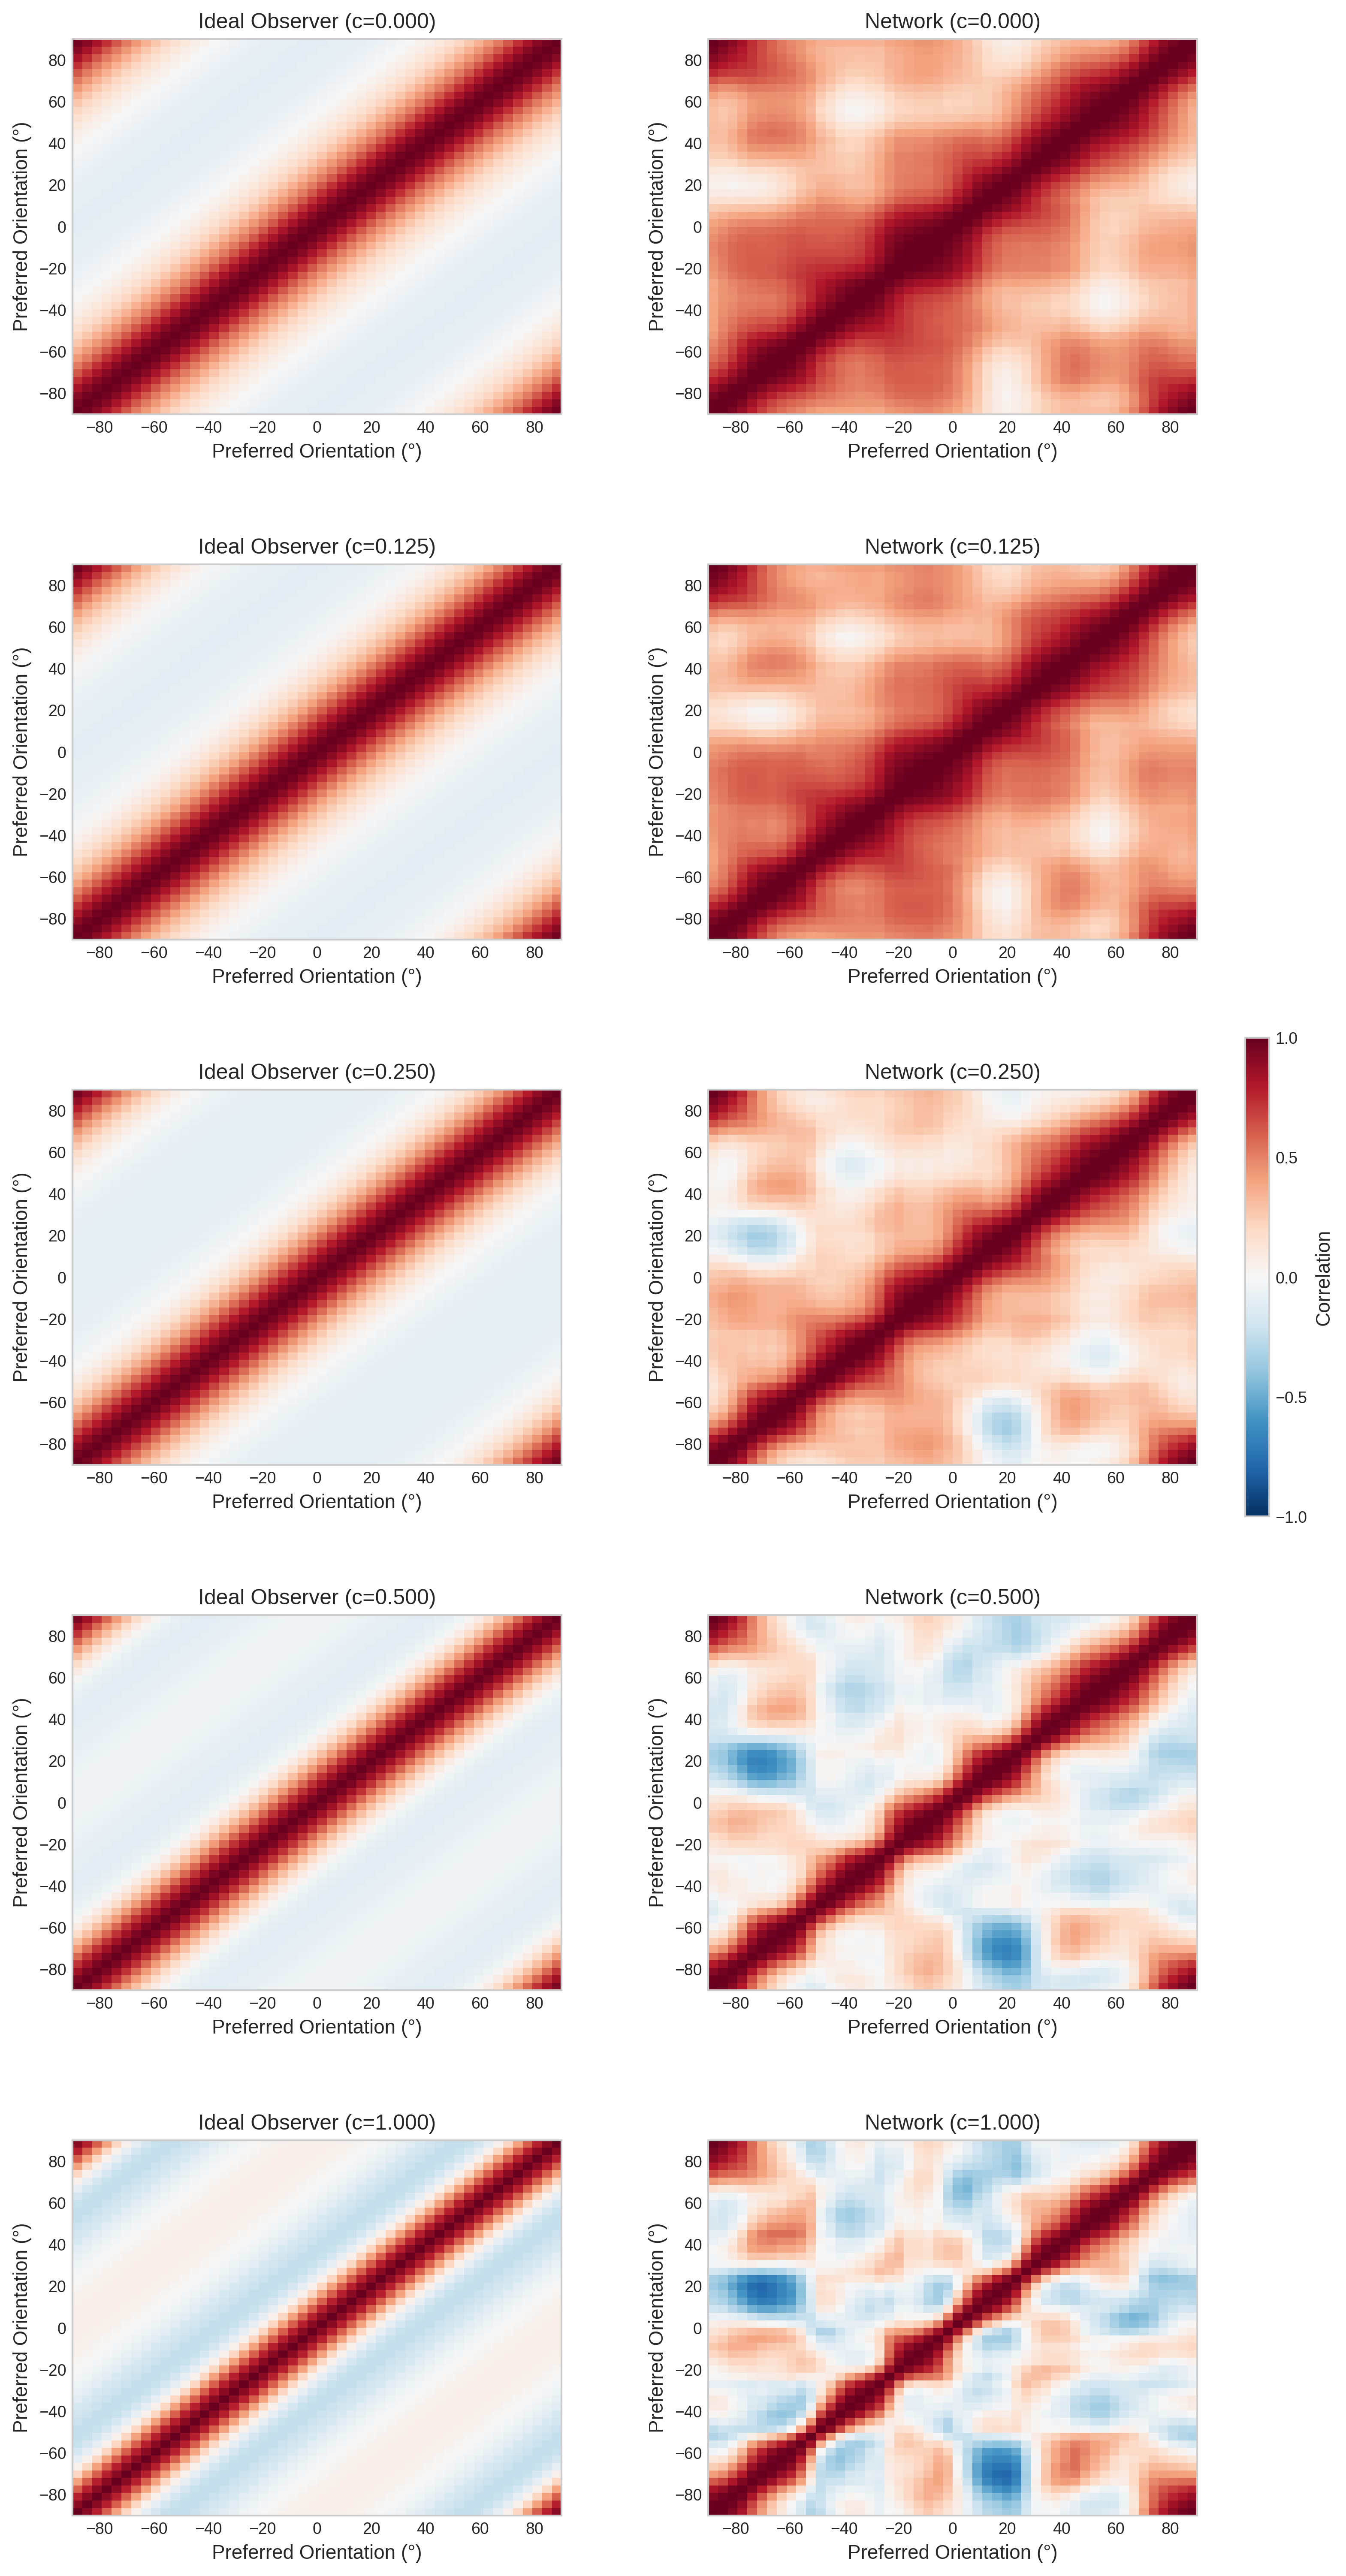
\includegraphics[width=0.6\textwidth]{08_resultados/figures/Fig2d_correlation_matrices.png}
    \caption{Matrices de correlación de Pearson entre potenciales de membrana excitatorios. Columna izquierda: observador ideal (\acrshort{GSM}). Columna derecha: red neuronal (\acrshort{SSN}). Cada columna corresponde a un nivel de contraste diferente.}
    \label{fig:fig2d}
\end{figure}


% \newgeometry{margin=0cm}
% \begin{figure}[!p]
%     \centering
%     % Imagen a página completa
%     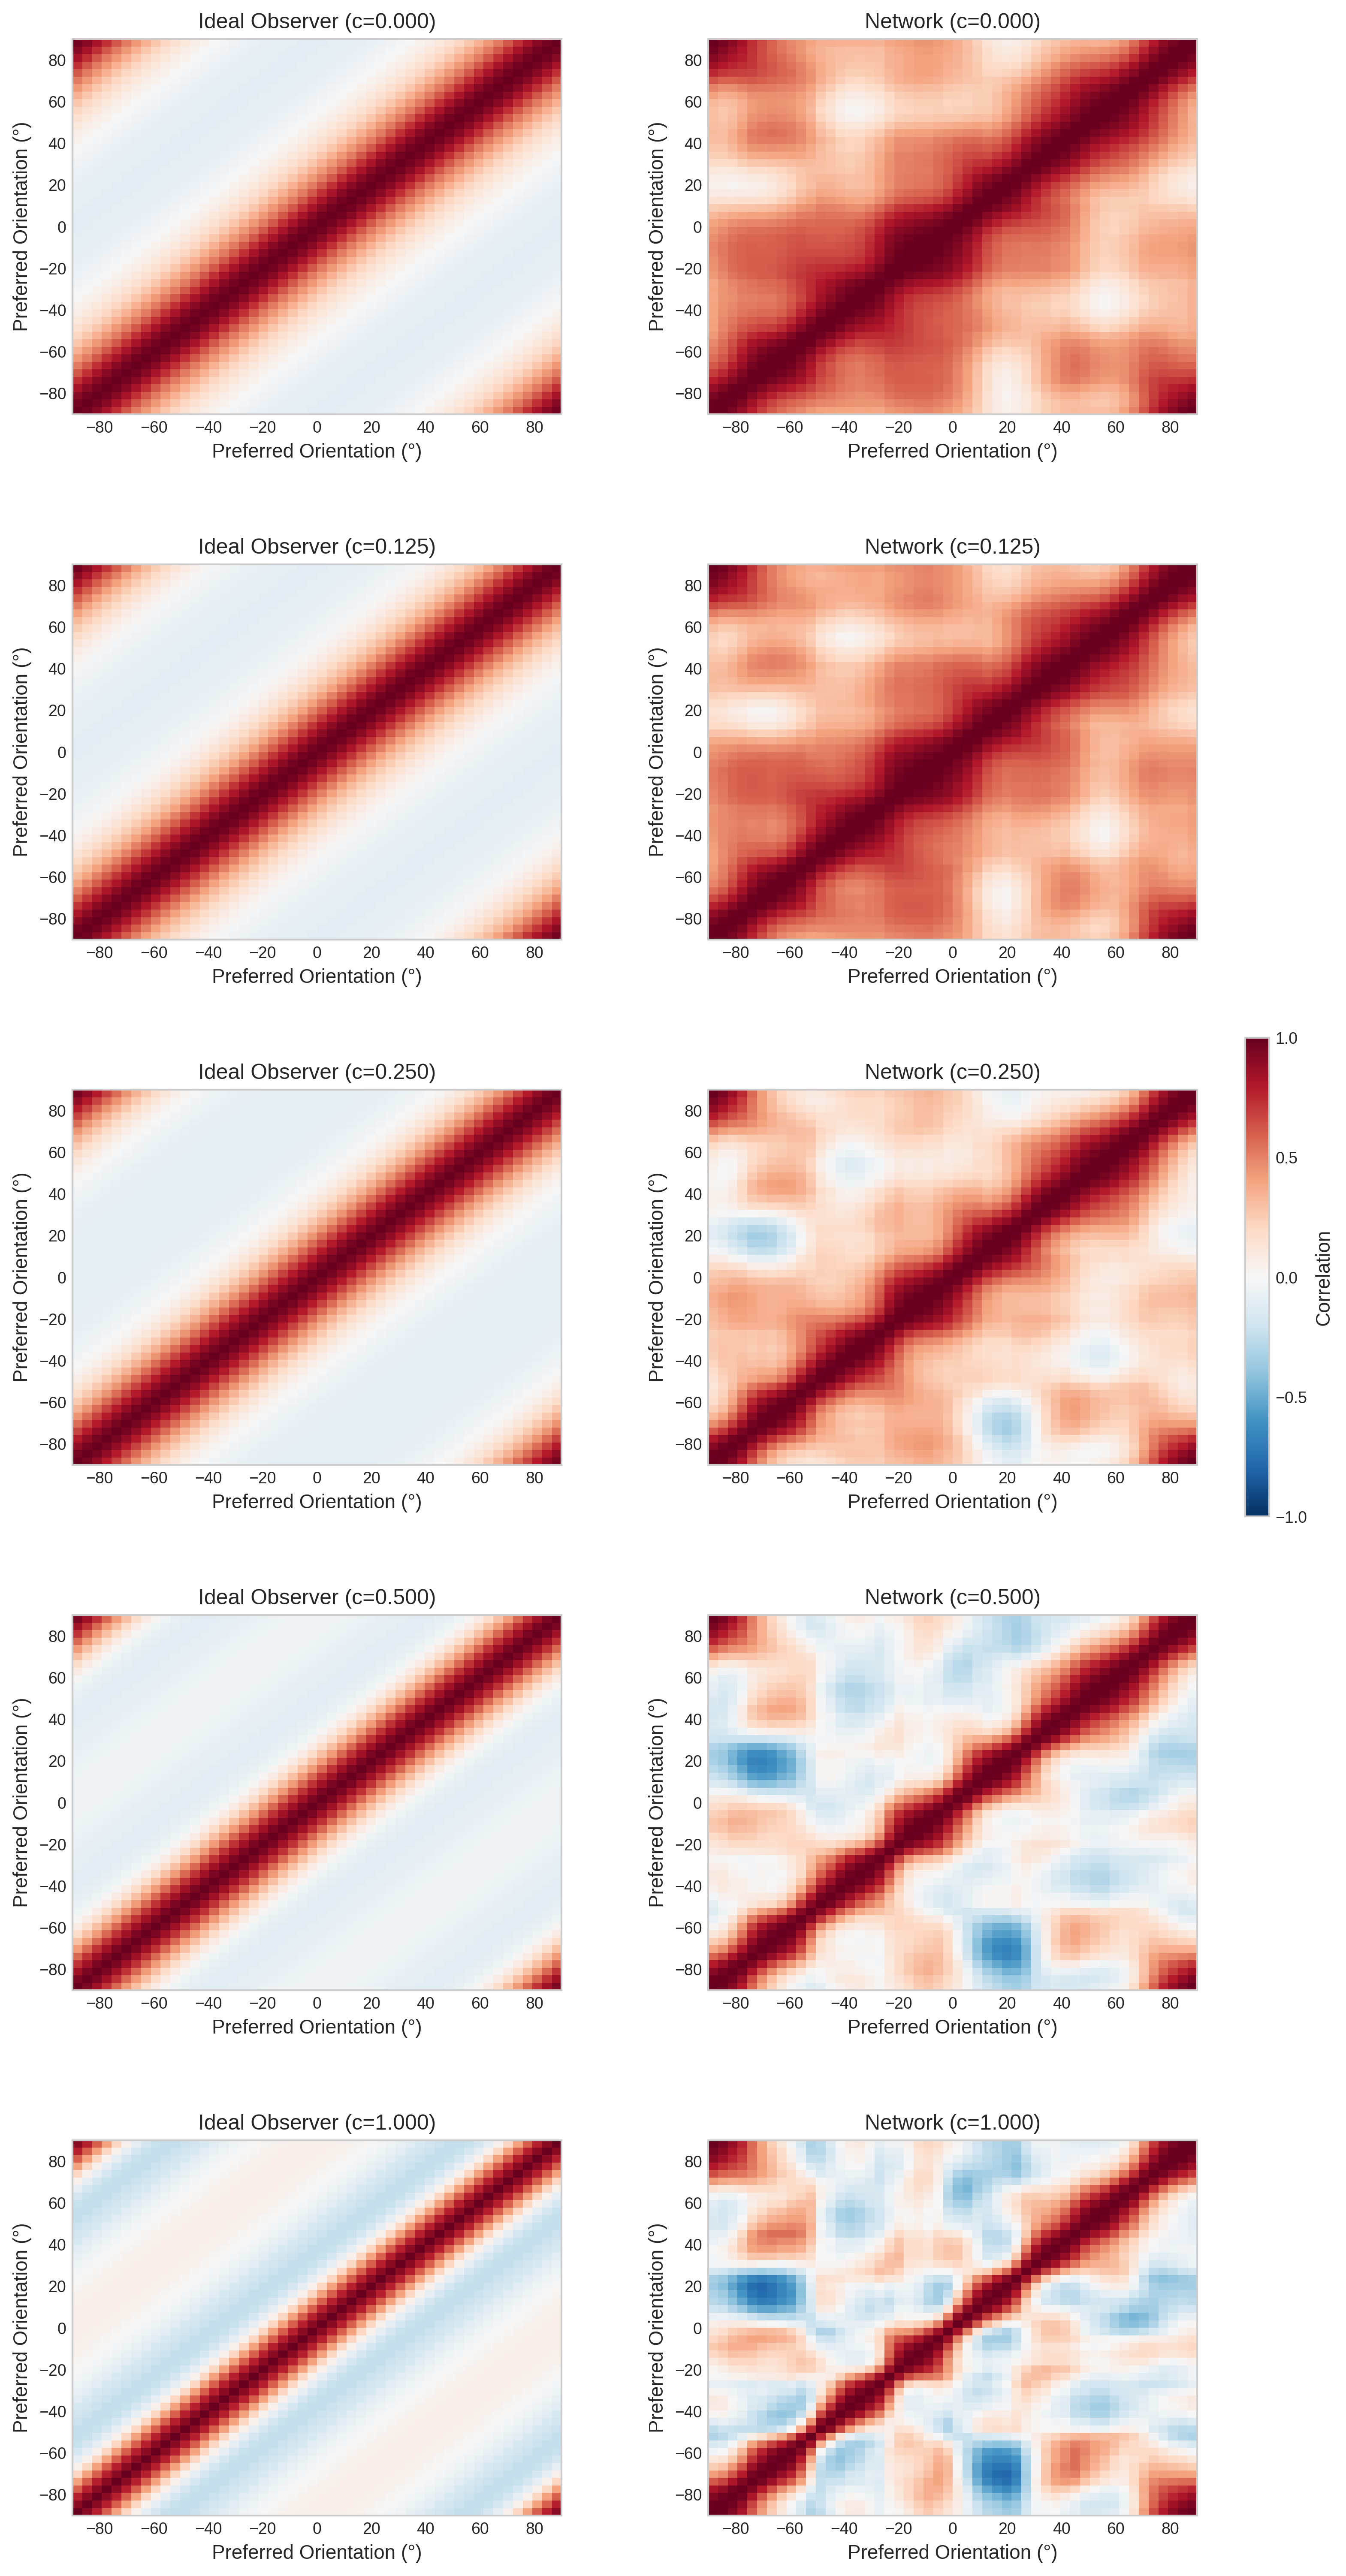
\includegraphics[height=0.8\paperheight,keepaspectratio]{08_resultados/figures/Fig2d_correlation_matrices.png}

%     % Caption limitada al ancho del texto
%     \vspace{2em}
%     \parbox{0.7\textwidth}{
%         \caption{Matrices de correlación de Pearson entre potenciales de membrana excitatorios. Columna izquierda: observador ideal (\acrshort{GSM}). Columna derecha: red neuronal (\acrshort{SSN}). Cada columna corresponde a un nivel de contraste diferente.}
%         \label{fig:fig2d}
%     }
% \end{figure}
% \restoregeometry



La diagonal principal muestra máxima correlación, y a medida que nos alejamos de la diagonal, la correlación decae gradualmente, reflejando que neuronas con orientaciones preferidas más distantes están menos correlacionadas. La estructura de correlaciones se modifica con el contraste de manera consistente entre el observador ideal y la red: para contraste cero, las correlaciones están determinadas principalmente por el prior del \acrshort{GSM}, mientras que con el aumento del contraste, la estructura refleja progresivamente más la información del estímulo. Calculando la correlación de Pearson elemento por elemento entre ambas matrices, se obtienen valores superiores a 0.95 para todos los niveles de contraste.

% =============================================================================
% SECCIÓN 4: ANÁLISIS DE PROPIEDADES DINÁMICAS
% =============================================================================

\section{Propiedades dinámicas emergentes}
\label{sec:res_dynamics}

Más allá de reproducir los momentos estadísticos correctos, el modelo de Echeveste se distingue por exhibir propiedades dinámicas que emergen como consecuencia del objetivo de muestreo sin ser explícitamente impuestas durante el entrenamiento. Esta sección presenta evidencia preliminar de que nuestra implementación preserva estas características, junto con las direcciones de trabajo futuro necesarias para una validación completa.

\subsection{Variabilidad modulada por estímulo}
\label{subsec:res_fano}

El fenómeno de quenching de variabilidad puede cuantificarse mediante el factor de Fano\footnote{El factor de Fano es una medida 
adimensional de dispersión relativa, análoga al coeficiente de variación pero apropiada para 
procesos de conteo.}, definido como $F = \text{Var}[r] / \mathbb{E}[r]$. Para un proceso de Poisson, $F = 1$; valores menores indican variabilidad sub-poissoniana, característica de respuestas corticales bajo estimulación.

El análisis cuantitativo del factor de Fano a partir de los datos de simulación muestra una reducción sistemática con el aumento del contraste: para contraste $z = 0$, el factor de Fano promedio se encuentra en el rango $1.0 - 1.2$, mientras que para $z = 1$ decrece hacia valores en el rango $0.6 - 0.8$. Esta reducción es particularmente pronunciada para las neuronas cuya orientación preferida coincide con la del estímulo, consistente con observaciones experimentales en \acrshort{V1} de primates \citep{echeveste2020cortical}.


\subsection{Análisis de oscilaciones gamma}
  \label{subsec:res_gamma}
  Una propiedad emergente notable del modelo de \citet{echeveste2020cortical} es la presencia de
  oscilaciones en el rango gamma (30-80 Hz), cuya frecuencia pico aumenta con el contraste del
  estímulo. Esta característica no es impuesta durante el entrenamiento, sino que surge como
  consecuencia de optimizar la red para realizar muestreo de la distribución posterior del
  \acrshort{GSM}. La relevancia de este hallazgo radica en que las oscilaciones gamma se observan
  consistentemente en registros electrofisiológicos de la corteza visual primaria (\acrshort{V1}) de
  primates, sugiriendo que podrían ser un subproducto funcional del cómputo probabilístico más que un
  epifenómeno.

  \subsubsection{Potencial de campo local}
  El potencial de campo local (\acrshort{LFP}) es una señal electrofisiológica que refleja la 
  actividad sináptica agregada de poblaciones neuronales en la vecindad de un electrodo de registro 
  extracelular. A diferencia de los potenciales de acción, que capturan la actividad de neuronas 
  individuales, el \acrshort{LFP} representa principalmente las corrientes sinápticas sumadas de 
  cientos a miles de neuronas, proporcionando una medida de la dinámica poblacional. En registros 
  experimentales de \acrshort{V1}, el \acrshort{LFP} exhibe oscilaciones prominentes en el rango 
  gamma durante la presentación de estímulos visuales, cuyas propiedades espectrales varían 
  sistemáticamente con parámetros del estímulo como el contraste y la orientación.

  En el contexto del modelo, el \acrshort{LFP} se aproxima como el promedio de los potenciales de 
  membrana de las neuronas excitatorias:
  \begin{equation}
      \text{LFP}(t) = \frac{1}{N_E} \sum_{i=1}^{N_E} u_E^{(i)}(t)
  \end{equation}
  Esta definición captura la actividad colectiva de la población excitatoria, constituyendo un 
  análogo computacional de la señal medida experimentalmente. La elección de promediar únicamente 
  sobre neuronas excitatorias sigue la convención del trabajo original y refleja que las neuronas 
  piramidales (excitatorias) contribuyen predominantemente al \acrshort{LFP} debido a su geometría 
  dendrítica extendida.


  \subsubsection{Análisis espectral}
 Para caracterizar el contenido oscilatorio del \acrshort{LFP}, se calculó su espectro de potencia, 
que describe cómo se distribuye la energía de la señal entre sus diferentes componentes 
frecuenciales. Una señal con oscilaciones gamma prominentes exhibirá un pico en el espectro 
dentro del rango 30-80 Hz.

La estimación espectral se realizó mediante el método de Welch, una técnica estándar en el 
análisis de señales neurofisiológicas. Este método divide la señal temporal en segmentos 
superpuestos, calcula el espectro de cada segmento individualmente, y promedia los resultados. 
El promediado reduce la variabilidad del estimador a costa de cierta pérdida en resolución 
frecuencial, proporcionando estimaciones más estables que las obtenidas a partir de la señal 
completa. En nuestro análisis, se utilizaron ventanas de Hanning con 50\% de solapamiento, 
parámetros comúnmente empleados en estudios de \acrshort{LFP} cortical.

La frecuencia pico gamma se identificó como el máximo del espectro dentro del rango 30-80 Hz 
para cada condición de contraste.

  \subsubsection{Resultados}
  La Figura~\ref{fig:gamma_analysis} presenta los resultados del análisis espectral para los cinco 
  niveles de contraste del conjunto de entrenamiento. Los paneles individuales muestran el espectro 
  de potencia en escala logarítmica, donde la banda sombreada indica el rango gamma (30-80 Hz) y las
  líneas punteadas marcan la frecuencia pico detectada dentro de este rango. El panel inferior 
  derecho sintetiza el resultado principal: la frecuencia pico gamma en función del contraste.
  \begin{figure}[!ht]
      \centering
      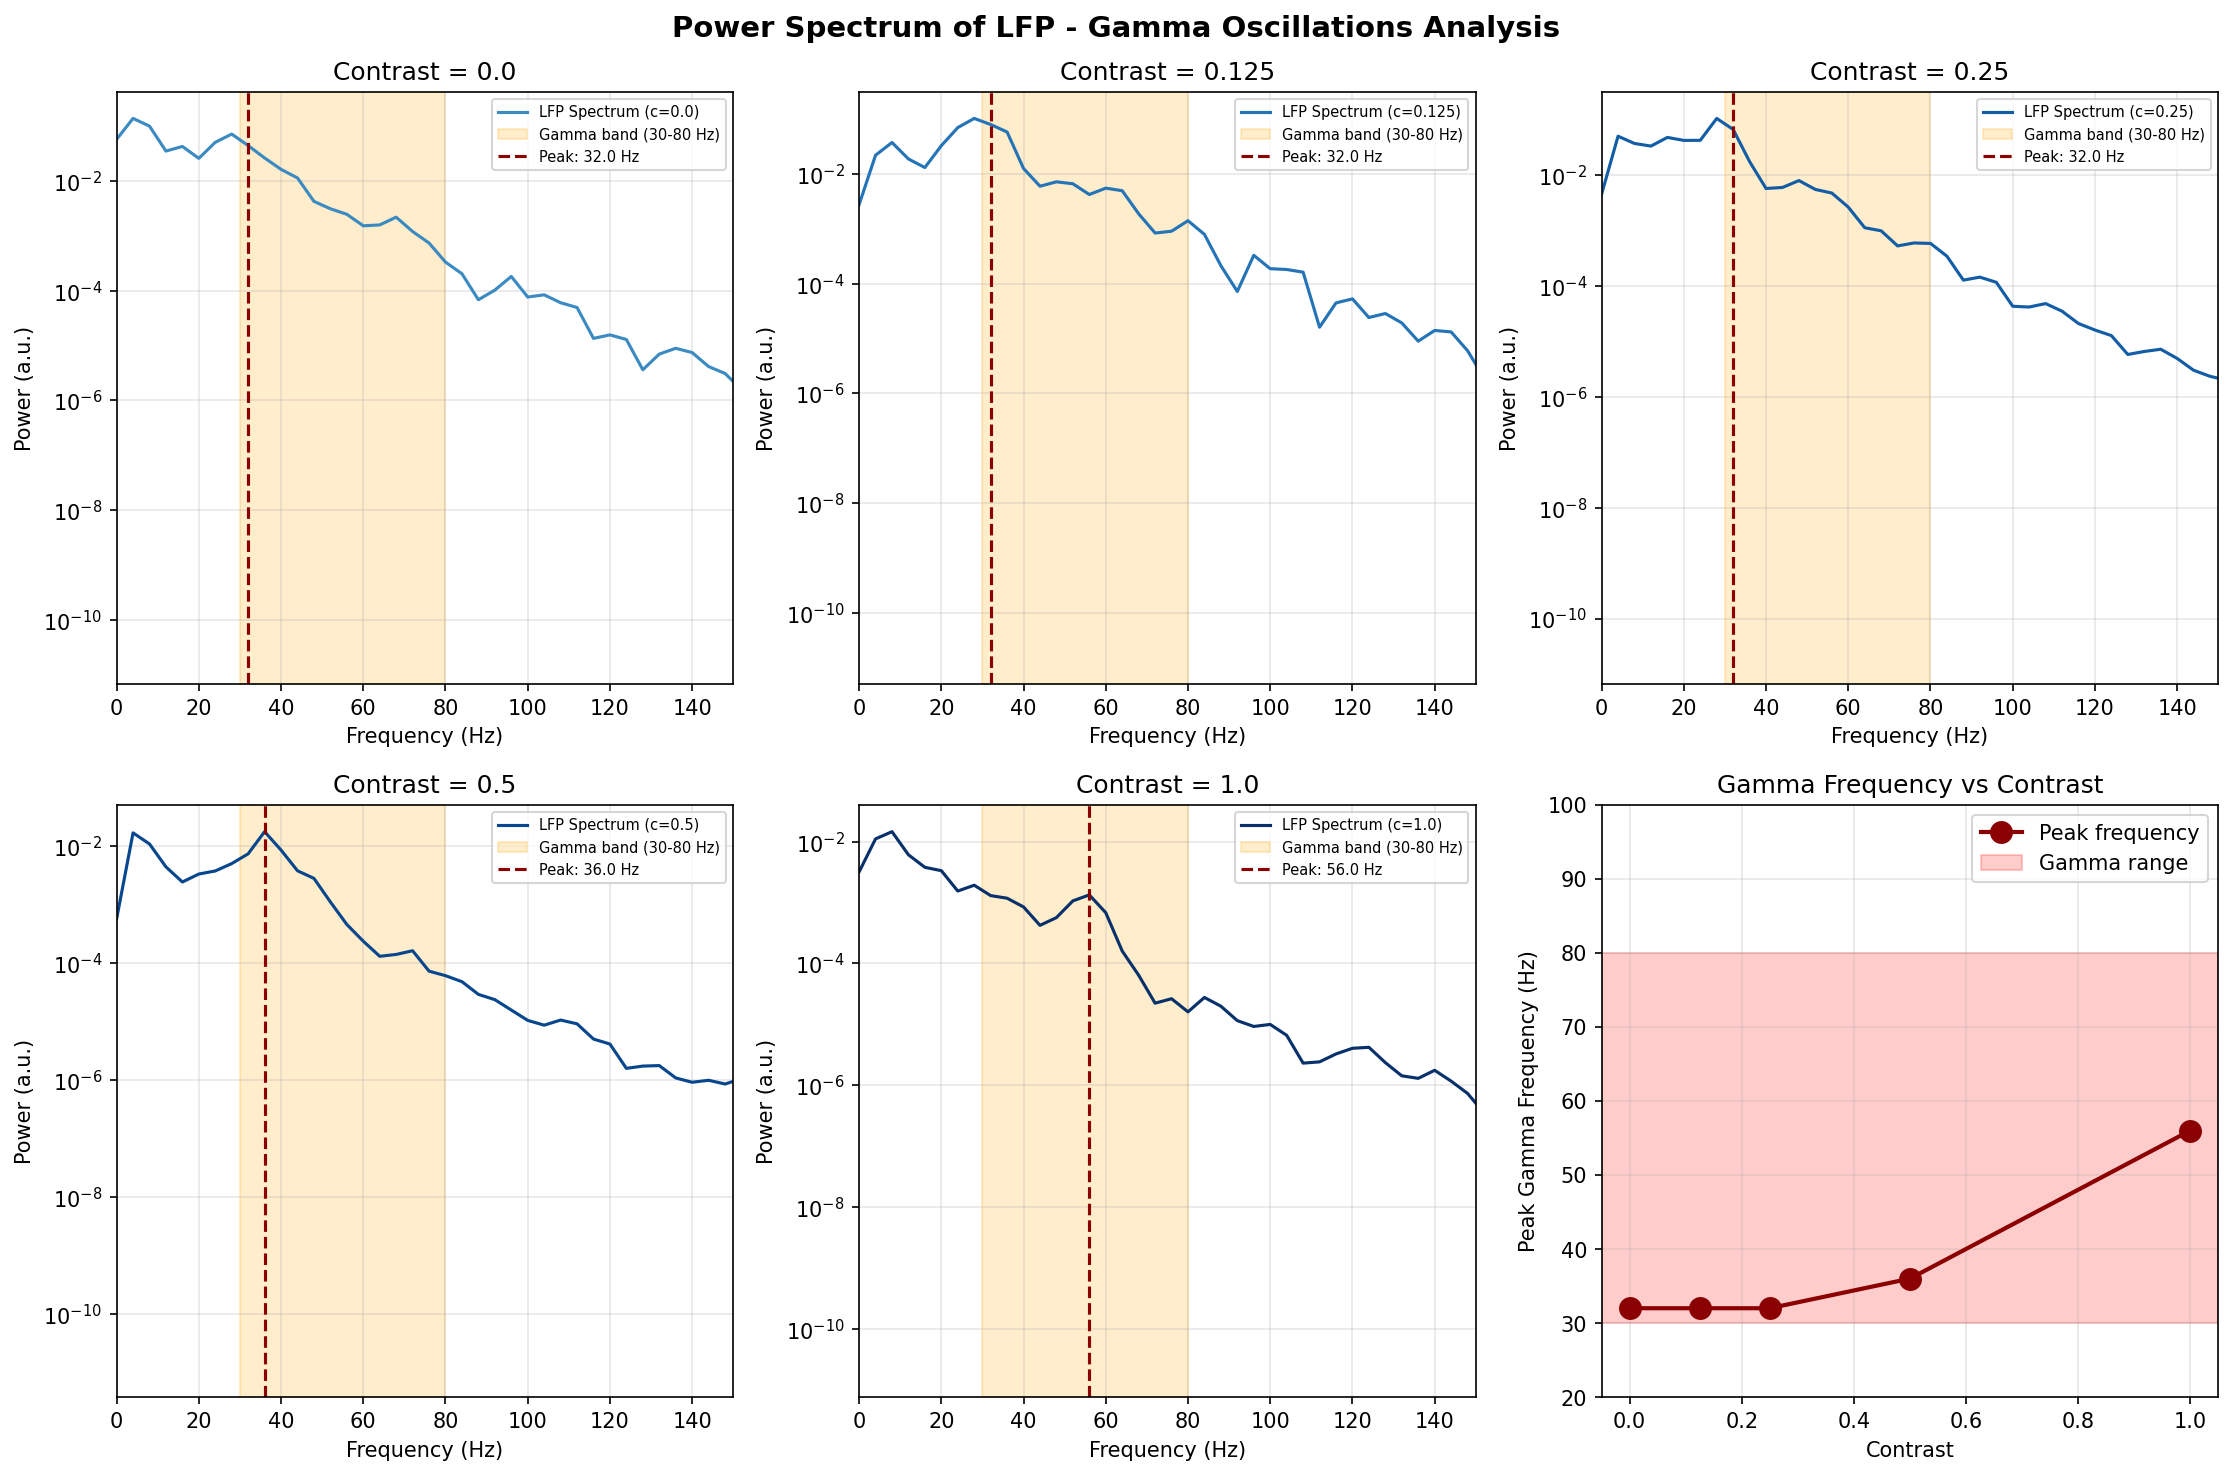
\includegraphics[width=0.95\textwidth]{08_resultados/figures/gamma_oscillations_analysis.png}
      \caption{Análisis espectral del potencial de campo local (\acrshort{LFP}). Los cinco primeros 
      paneles muestran el espectro de potencia para cada nivel de contraste, con la banda gamma 
      (30-80 Hz) sombreada en rojo y la frecuencia pico indicada con línea punteada. El panel 
      inferior derecho muestra la dependencia de la frecuencia pico con el contraste, confirmando 
      el incremento predicho por el modelo: de aproximadamente 32 Hz (contraste bajo) a 56 Hz 
      (contraste máximo).}
      \label{fig:gamma_analysis}
  \end{figure}
  Los resultados confirman que la red implementada reproduce la fenomenología reportada en el 
  artículo original. Para contraste nulo o bajo ($z \leq 0.25$), la frecuencia pico se mantiene 
  alrededor de 32 Hz, correspondiente al extremo inferior del rango gamma. A medida que el contraste 
  aumenta, la frecuencia pico se desplaza progresivamente hacia valores más altos, alcanzando 
  aproximadamente 56 Hz para contraste máximo ($z = 1.0$). Este comportamiento es cualitativamente 
  consistente con observaciones experimentales en \acrshort{V1}, donde se ha reportado que la 
  frecuencia de oscilaciones gamma aumenta con el contraste del estímulo visual 
  \citep{echeveste2020cortical}.

  Desde una perspectiva computacional, este fenómeno puede interpretarse en términos de la dinámica 
  de muestreo: mayor contraste implica mayor certeza sobre el estímulo (menor varianza posterior), 
  lo que permite a la red explorar el espacio de estados más rápidamente, manifestándose como 
  oscilaciones de mayor frecuencia. Esta interpretación conecta las propiedades espectrales 
  observadas con la función de inferencia probabilística que la red implementa.

% \subsection{Transitorios al inicio del estímulo}
% \label{subsec:res_transients}

% Los overshoots transitorios al inicio del estímulo representan otra propiedad emergente del modelo que cumple un rol funcional en la reducción del tiempo de burn-in para la inferencia. Simulaciones preliminares utilizando el modo \texttt{three\_phase} muestran indicios de respuestas transitorias consistentes con las predicciones teóricas.

% \subsection{Validaciones pendientes}
% \label{subsec:res_pending}

% Para completar la validación según los estándares establecidos por \citet{echeveste2020cortical}, se identifican las siguientes direcciones de trabajo futuro:

% \textbf{Pruebas de generalización} (Figura 3 del artículo original): verificación de que la red interpola correctamente a niveles de contraste no entrenados, y evaluación del rendimiento con un conjunto de 500 estímulos nuevos generados por el \acrshort{GSM} que incluyen múltiples orientaciones dominantes.

% \textbf{Análisis espectral completo}: verificación de oscilaciones gamma mediante análisis de potencia espectral del potencial de campo local (\acrshort{LFP}), incluyendo la dependencia de la frecuencia pico con el contraste.

% \textbf{Redes de control}: el artículo original entrena múltiples redes que difieren en un único aspecto (sin modulación de covarianza, sin principio de Dale, sin penalización de slowness, con factores de Fano constantes), demostrando la necesidad de cada componente. La implementación de estas comparaciones constituye una validación importante.

% \textbf{Comparación con datos experimentales} (Figura 7): validación de que las propiedades de la red optimizada son consistentes con registros electrofisiológicos de \acrshort{V1} en primates.

% =============================================================================
% SECCIÓN 5: RESUMEN
% =============================================================================

\section{Resumen del capítulo}
\label{sec:res_summary}

Este capítulo presentó los resultados de la validación de nuestra implementación del modelo de \citet{echeveste2020cortical} en múltiples niveles. La validación función por función demostró equivalencia numérica exacta con errores del orden de la precisión de punto flotante ($\sim 10^{-15}$). Las pruebas unitarias verificaron la correctitud de componentes individuales. El procedimiento de entrenamiento demostró convergencia robusta hacia parámetros comparables a los de referencia. Las simulaciones replicaron las figuras centrales del artículo original, confirmando que la red implementa correctamente muestreo de la distribución posterior del modelo generativo \acrshort{GSM}.

Estos resultados establecen que la implementación está lista para su uso en investigaciones que requieran un modelo de dinámicas corticales biológicamente realistas para inferencia probabilística unimodal. Las validaciones pendientes identificadas, particularmente respecto a generalización, análisis espectral y redes de control, definen direcciones claras para trabajo futuro. \cleardoublepage
\chapter{Conclusiones y trabajo a futuro}
\label{chapter:conclu}

En este trabajo llevamos a cabo la implementación completa del modelo de \citet{echeveste2020cortical} dentro del framework Scikit-NeuroMSI, estableciendo las bases técnicas necesarias para futuras investigaciones que combinen dinámicas corticales realistas con integración multisensorial. Esta implementación representa el primer paso hacia una visión más amplia: el desarrollo de modelos que unifiquen la arquitectura multimodal del enfoque de Cuppini con los mecanismos de muestreo estocástico del modelo de Echeveste.

La reimplementación del código original, que se encontraba en OCaml, requirió una traducción completa a Python utilizando JAX para diferenciación automática. Este proceso, aunque inicialmente inesperado, resultó en una implementación moderna compatible con el ecosistema actual de herramientas de neurociencia computacional, con soporte transparente para aceleración en \acrshort{GPU} y una arquitectura modular que facilita futuras extensiones.

La validación de la implementación se realizó en múltiples niveles complementarios. La verificación función por función demostró equivalencia numérica exacta con el código original, alcanzando errores del orden de la precisión de punto flotante ($\sim 10^{-15}$). Las pruebas del procedimiento de entrenamiento confirmaron que los parámetros optimizados convergen hacia valores comparables a los de referencia, con múltiples corridas independientes mostrando consistencia en los resultados. Las simulaciones replicaron las figuras centrales del artículo original, verificando que la red implementada reproduce correctamente las propiedades de inferencia probabilística mediante muestreo y las dinámicas temporales características, incluyendo oscilaciones gamma cuya frecuencia aumenta con el contraste del estímulo.

Como contribuciones adicionales al framework, se desarrollaron dos paquetes nuevos: \texttt{data} que proporciona infraestructura para gestionar parámetros pre-entrenados y componentes de modelos generativos, y \texttt{generative} que introduce por primera vez modelos generativos como el \acrshort{GSM} al framework. Este último módulo fue diseñado con extensibilidad en mente, permitiendo incorporar futuros modelos generativos siguiendo la misma interfaz.


% Es importante reconocer las limitaciones del presente trabajo. La implementación se centró exclusivamente en el modelo unimodal de Echeveste, sin abordar la fusión con el modelo de Cuppini ni la implementación de inferencia causal multisensorial. Estas extensiones, que constituían la motivación inicial del proyecto, requieren resolver desafíos técnicos y conceptuales adicionales que exceden el alcance de esta tesis.
% TODO: Acá tendrías que ser más específico para mencionar por qué excede el alcance, si inicialmente fue tu objetivo. O sea, sabemos que te faltó tiempo, recursos, etc, pero debes dejarlo claro. Si no, suena a que tiene problemas que están fuera de tu alcance. Vale la pena ser más detallado para explicar a qué te refieres con desafíos técnios y conceptuales. Si no, suena a chamuyo.

Es importante reconocer las limitaciones del presente trabajo. La implementación se centró exclusivamente en el modelo unimodal de Echeveste, sin abordar la fusión con el modelo de Cuppini ni la implementación de inferencia causal multisensorial. Estas extensiones, que constituían la motivación inicial del proyecto, quedaron fuera del alcance de esta tesis porque la implementación del modelo de Echeveste resultó ser un trabajo considerablemente mayor al anticipado. Lo que inicialmente se planteó como una adaptación relativamente directa se transformó en un desarrollo de gran tamaño, el descubrimiento de que el código de entrenamiento original estaba escrito en OCaml requirió una reimplementación completa desde cero, la integración con el framework demandó resolver incompatibilidades de diseño no previstas, y cada componente del modelo (el \acrshort{GSM}, las dinámicas de la red, el procedimiento de entrenamiento, la visualización de resultados) presentó problemas técnicos propios que fueron expandiendo progresivamente el volumen de trabajo. El resultado fue una implementación más extensa y compleja de lo planificado, pero también más completa y rigurosa. Todo esto teniendo en cuenta que la implementación validada que aquí presentamos constituye una condición necesaria para cualquier desarrollo futuro en esa dirección.


% Como resultado, la implementación del modelo de Echeveste convierte a Scikit-NeuroMSI en una plataforma más completa para el estudio de modelos neurocomputacionales, incorporando por primera vez un modelo con dinámicas corticales basadas en muestreo estocástico. Esta contribución no solo beneficia a quienes deseen utilizar específicamente este modelo, sino que establece patrones y herramientas que pueden ser aprovechados para la implementación de modelos similares en el futuro.
% TODO: ¿Qué modelos por ejemplo? Acá es donde debes citar, para que quede claro a qué literatura científica vas a aportar.
Como resultado, la implementación del modelo de Echeveste convierte a Scikit-NeuroMSI en una plataforma más completa para el estudio de modelos neurocomputacionales, incorporando por primera vez un modelo con dinámicas corticales basadas en muestreo estocástico. Esta contribución no solo beneficia a quienes deseen utilizar específicamente este modelo, sino que establece patrones y herramientas que pueden ser aprovechados para la implementación de modelos similares. Por ejemplo, el trabajo de \citet{ursino2017multisensory} demostró que las sinapsis cross-modales del modelo de Cuppini pueden entrenarse mediante aprendizaje hebbiano para reflejar conocimiento a priori sobre la co-ocurrencia de estímulos; una extensión natural sería incorporar este mecanismo de maduración sináptica dentro del framework. De manera análoga, el modelo de \citet{haefner2016perceptual}, que extiende el paradigma de muestreo neuronal a la toma de decisiones perceptuales, representa otro candidato para implementación en Scikit-NeuroMSI aprovechando la infraestructura que aquí desarrollamos para modelos basados en muestreo estocástico.


Más allá de su contribución técnica específica, este trabajo se enmarca en una perspectiva más amplia sobre el rol de los modelos biológicamente plausibles tanto en la comprensión del cerebro como en el futuro de la neurociencia computacional. Actualmente existe una brecha profunda entre las redes neuronales artificiales, optimizadas exclusivamente para maximizar rendimiento en tareas específicas, y los circuitos neuronales biológicos que exhiben propiedades como estocasticidad, dinámicas oscilatorias, y estricto balance entre excitación e inhibición. El modelo de Echeveste demuestra que estas propiedades biológicas no son meros epifenómenos evolutivos sino que cumplen roles computacionales precisos: las oscilaciones gamma que emerge de la red entrenada aceleran la exploración del espacio de estados \citep{echeveste2020cortical}, y la variabilidad neuronal codifica la incertidumbre de la distribución posterior del modelo generativo \citep{echeveste2020cortical}. Estos resultados se suman a evidencia previa mostrando que la actividad espontánea cortical refleja propiedades estadísticas del modelo interno del entorno \citep{berkes2011spontaneous}, y que la variabilidad neuronal modulada por el estímulo es consistente con un mecanismo de muestreo probabilístico \citep{banyai2019stimulus}.

\section{Trabajo a futuro}

% La dirección más prometedora para trabajo futuro es la integración del modelo de Echeveste con el modelo de Cuppini ya implementado en Scikit-NeuroMSI. Esta fusión permitiría estudiar cómo fenómenos de integración multisensorial, como el efecto ventrílocuo, emergen de circuitos neuronales que implementan inferencia probabilística mediante muestreo estocástico. Tal modelo unificado tendría implicaciones tanto teóricas, demostrando que los principios de muestreo neuronal pueden extenderse al dominio multisensorial, como prácticas, permitiendo conectar predicciones del modelo con observaciones electrofisiológicas reales de integración audiovisual.

% TODO: ¿Realmente sería la primera vez que se hace algo así? ¿El modelo de Ursino no es algo parecido? Debes ser más preciso en qué aspecto reside la innovación. Sugiero que puedas mencionar también la literatura en neurociencias sobre ondas EEG e integración multisensorial. Ahí vas a encontrar detalles sobre las ondas beta, gamma, que pueden ser asociados al paradigma del ventrículo espacial. Mira textos de Romei por ejemplo, o en mis papers las referencias. Tu innovación sería esa. Puedes modelar directamente las ondas cerebrales asociadas a la integración multisensorial! Eso sí no se ha hecho antes que yo sepa.

La dirección más prometedora para trabajo futuro es la integración del modelo de Echeveste con el modelo de Cuppini ya implementado en Scikit-NeuroMSI. Esta fusión permitiría estudiar cómo fenómenos de integración multisensorial, como el efecto ventrílocuo, emergen de circuitos neuronales que implementan inferencia probabilística mediante muestreo estocástico. Trabajos previos del grupo de Ursino ya han avanzado en direcciones relevantes, \citet{ursino2009recognition} exploraron el rol de la sincronización gamma en el reconocimiento de objetos mediante osciladores neuronales, y \citet{ursino2017multisensory} demostraron que las sinapsis cross-modales del modelo de Cuppini pueden aprenderse mediante maduración hebbiana, incorporando conocimiento a priori sobre la co-ocurrencia de estímulos. La fusión que proponemos busca llevar estos avances un paso más allá, incorporando dinámicas corticales basadas en muestreo estocástico con balance excitación-inhibición al dominio multisensorial. A diferencia de los modelos deterministas de tasa existentes, un modelo así generaría señales de \acrshort{LFP} simuladas con oscilaciones emergentes en bandas fisiológicamente relevantes (gamma, beta, theta), lo que abriría la posibilidad de modelar directamente las dinámicas oscilatorias cerebrales asociadas a la integración multisensorial y contrastarlas con registros electrofisiológicos reales de tareas como la ventriloquía espacial.

Aunque nuestra implementación reproduce y verifica varias propiedades reportadas en el artículo original, una línea complementaria de trabajo futuro consiste en extender la validación experimental del modelo. Este tipo de validaciones tiene precedentes claros, donde por ejemplo, \citet{echeveste2020cortical} entrenaron redes de control que diferían en un único aspecto (sin modulación de covarianza, sin principio de Dale, sin penalización de slowness) para demostrar la necesidad de cada componente, y \citet{banyai2019stimulus} realizaron análisis detallados de cómo la complejidad del estímulo modula las correlaciones de respuesta en \acrshort{V1}. Replicar estas comparaciones con nuestra implementación fortalecería la confianza en el código y proporcionaría insights adicionales sobre los mecanismos subyacentes.



% Una línea de trabajo futuro relevante para la arquitectura del framework es la reestructuración de la presentación de estímulos a los modelos. Durante la implementación del \acrshort{GSM}, los estímulos quedaron parcialmente desacoplados del modelo neuronal, lo cual representa un paso en la dirección correcta. Sin embargo, sería beneficioso formalizar esta separación de manera más sistemática, estableciendo una interfaz clara entre la generación de estímulos y los modelos que los procesan. Esta abstracción permitiría intercambiar diferentes tipos de estímulos (visuales, auditivos, multimodales) sin modificar la lógica interna de los modelos, facilitando tanto la experimentación con diferentes paradigmas como la eventual integración de múltiples modalidades sensoriales en un mismo marco computacional.
% TODO: Acá cita de nuevo nuestro paper de scikirneuromsi, esa idea no es tuya completamente.

Una línea de trabajo futuro relevante planteada por \citeauthor{paredes2025scikit} para la arquitectura del framework es la reestructuración de la presentación de estímulos a los modelos. En nuestro caso, durante la implementación del \acrshort{GSM}, los estímulos quedaron parcialmente desacoplados del modelo neuronal, lo cual representa un paso en la dirección correcta. Sin embargo, como señalan \citet{paredes2025scikit}, sería beneficioso formalizar esta separación de manera más sistemática, estableciendo una interfaz clara entre la generación de estímulos y los modelos que los procesan. Esta abstracción permitiría intercambiar diferentes tipos de estímulos (visuales, auditivos, multimodales) sin modificar la lógica interna de los modelos, facilitando tanto la experimentación con diferentes paradigmas como la eventual integración de múltiples modalidades sensoriales en un mismo marco computacional.


% Otra extensión natural es la implementación de otros modelos generativos dentro del módulo \texttt{generative}. Modelos como campos aleatorios de Markov, modelos de energía, o modelos generativos multimodales podrían incorporarse siguiendo la interfaz establecida por el \acrshort{GSM}. Esta diversidad de modelos generativos permitiría estudiar cómo diferentes supuestos sobre la estructura estadística de los estímulos afectan las dinámicas de muestreo neuronal y las propiedades emergentes de los circuitos.
% TODO: Y por qué es importante incorporarlos? Cómo contribuyen al campo de la integración multisensorial? Citas.

Otra extensión natural es la implementación de otros modelos generativos dentro del módulo \texttt{generative}. Modelos como campos aleatorios de Markov o modelos generativos multimodales podrían incorporarse siguiendo la interfaz establecida por el \acrshort{GSM}. Esto resulta particularmente interesante porque, como mostró \citet{echeveste2020cortical}, las propiedades emergentes del circuito (frecuencia de oscilaciones gamma, magnitud de transitorios, estructura de correlaciones) dependen críticamente de los momentos objetivo derivados del modelo generativo. Disponer de múltiples modelos generativos permitiría investigar sistemáticamente cómo cambian estas dinámicas al modificar el problema de inferencia que la red debe resolver, extendiendo el análisis más allá del \acrshort{GSM} visual hacia representaciones que incluyan estructura causal multimodal, como las propuestas por \citet{kording2007causal}.



% Por último, consideramos relevante explorar la aplicación del modelo a datos experimentales reales. El marco teórico de muestreo neuronal genera predicciones específicas sobre la relación entre variabilidad neural, oscilaciones gamma, y propiedades del estímulo que podrían contrastarse con registros electrofisiológicos de corteza visual. Esta validación experimental constituiría el test más riguroso del modelo y podría revelar tanto sus fortalezas como sus limitaciones para capturar la complejidad de los circuitos corticales reales.
% TODO: ¿Qué datos experimentales? Cita los estudios que podrías reproducir.


Por último, consideramos relevante explorar la aplicación del modelo a datos experimentales reales. El marco teórico de muestreo neuronal genera predicciones específicas sobre la relación entre variabilidad neural, oscilaciones gamma y propiedades del estímulo. Estas predicciones podrían contrastarse con registros electrofisiológicos de corteza visual como los analizados por \citet{banyai2019stimulus}, quienes estudiaron cómo las correlaciones de respuesta en \acrshort{V1} dependen de la complejidad del estímulo, o con los datos de \citet{haefner2016perceptual}, que vincularon la variabilidad neuronal con decisiones perceptuales en un marco de muestreo probabilístico. Esta validación experimental constituiría el test más exigente del modelo y podría revelar tanto las condiciones en que el paradigma de muestreo captura adecuadamente la dinámica cortical como aquellas en que resulta insuficiente.










 \cleardoublepage
\appendix
\chapter{Material complementario}
\label{appendix:validation}

Este apéndice contiene diagramas técnicos y tablas de mayor detalle que complementan las explicaciones de los capítulos anteriores. Estas figuras proporcionan una visión más exhaustiva de la arquitectura de software, los flujos de ejecución y los resultados de validación, lo que resulta útil para lectores interesados en comprender o extender la implementación.

%=============================================================================
%=============================================================================

% --- FIGURA 1: DIAGRAMA DE COMPONENTES ---
\begin{figure}[H]
    \centering
    \makebox[\textwidth][c]{
        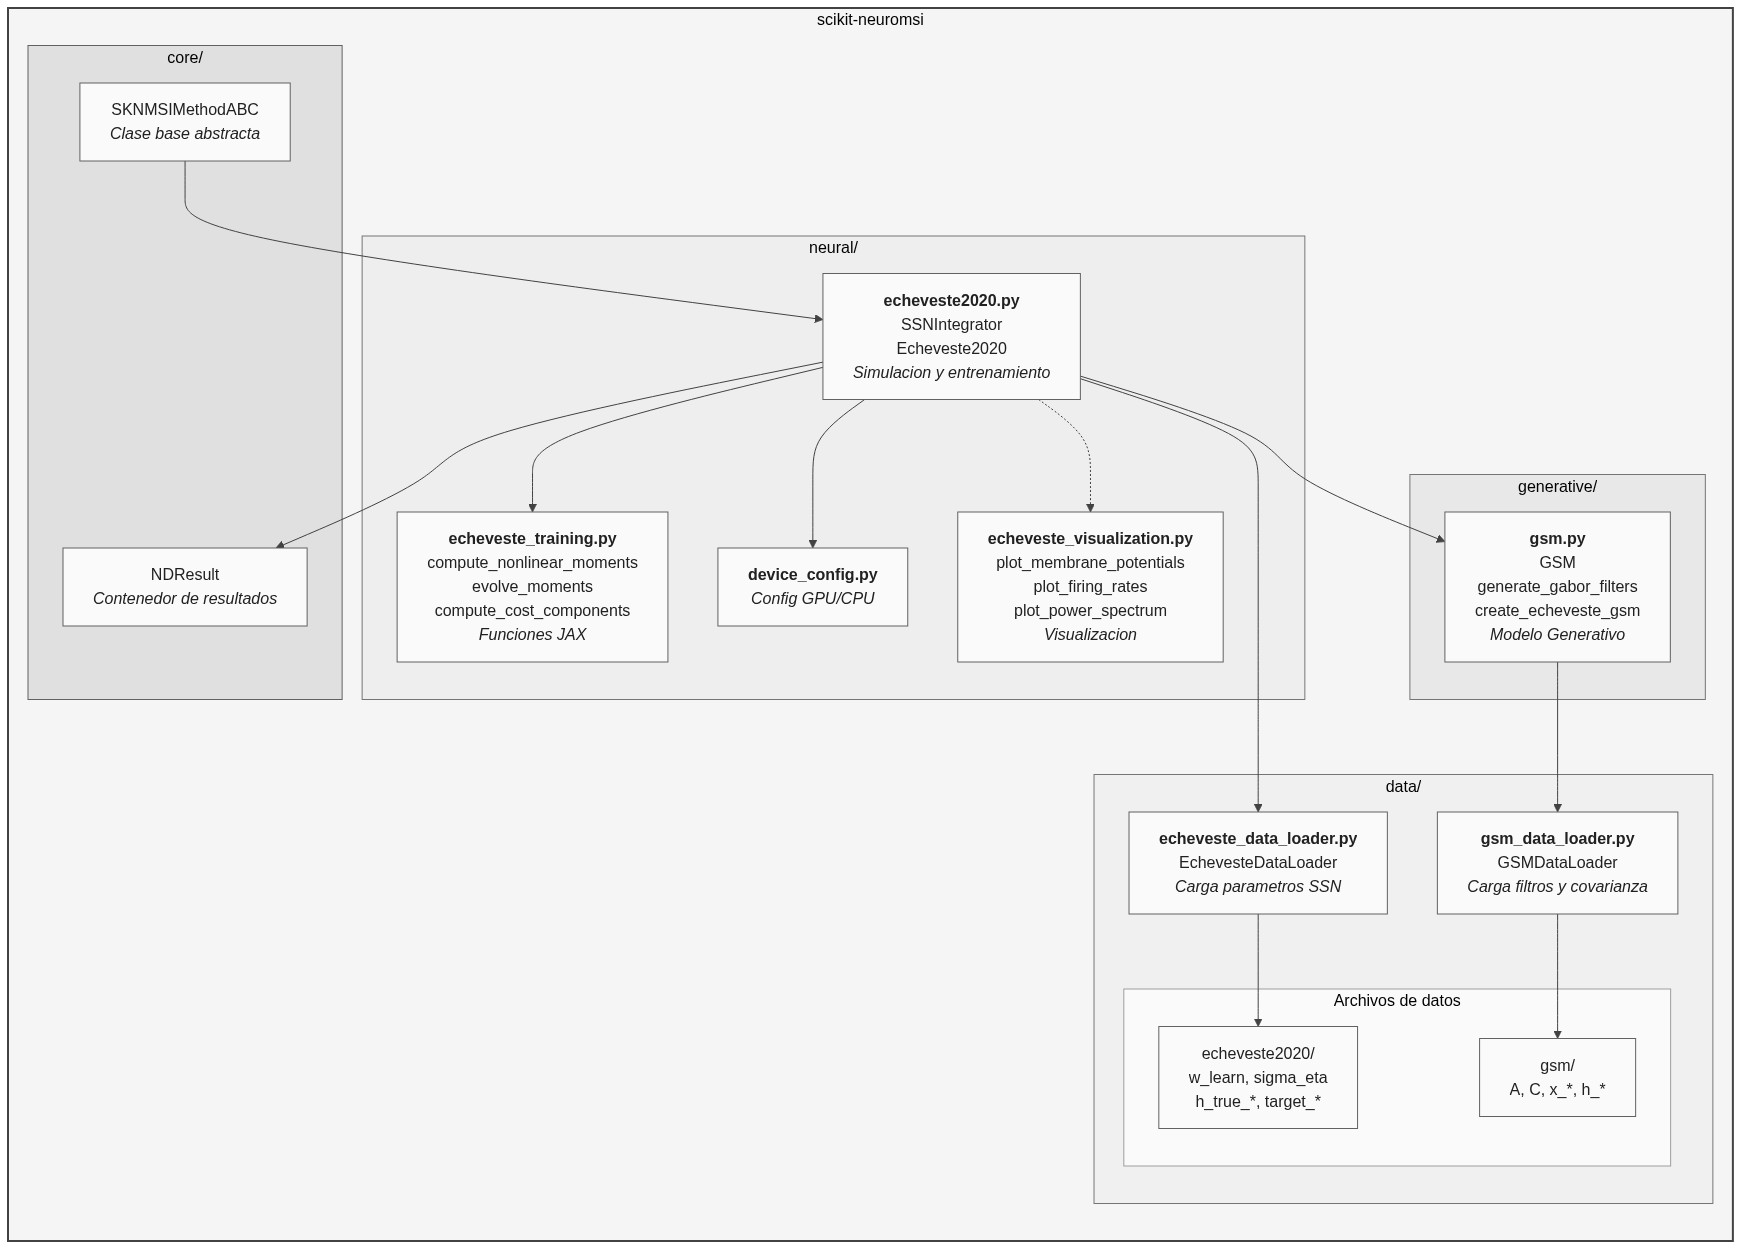
\includegraphics[width=1.3\textwidth]{10_apendice/figures/03_component_diagram_simplified.png}
    }
    \caption{
        Estructura modular del paquete scikit-neuromsi. Se detalla la organización del código en submódulos especializados: el núcleo (\texttt{core/}) con la clase base abstracta y el contenedor de resultados, el módulo neuronal (\texttt{neural/}) con las clases de simulación y las funciones de entrenamiento en JAX, el módulo generativo (\texttt{generative/}) con el modelo \acrshort{GSM}, y el sistema de gestión de datos (\texttt{data/}) con los cargadores especializados.
    }
    \label{fig:component-diagram}
\end{figure}

% --- FIGURA 2: DIAGRAMA DE CLASES ---
\begin{figure}[H]
    \centering
    \makebox[\textwidth][c]{
        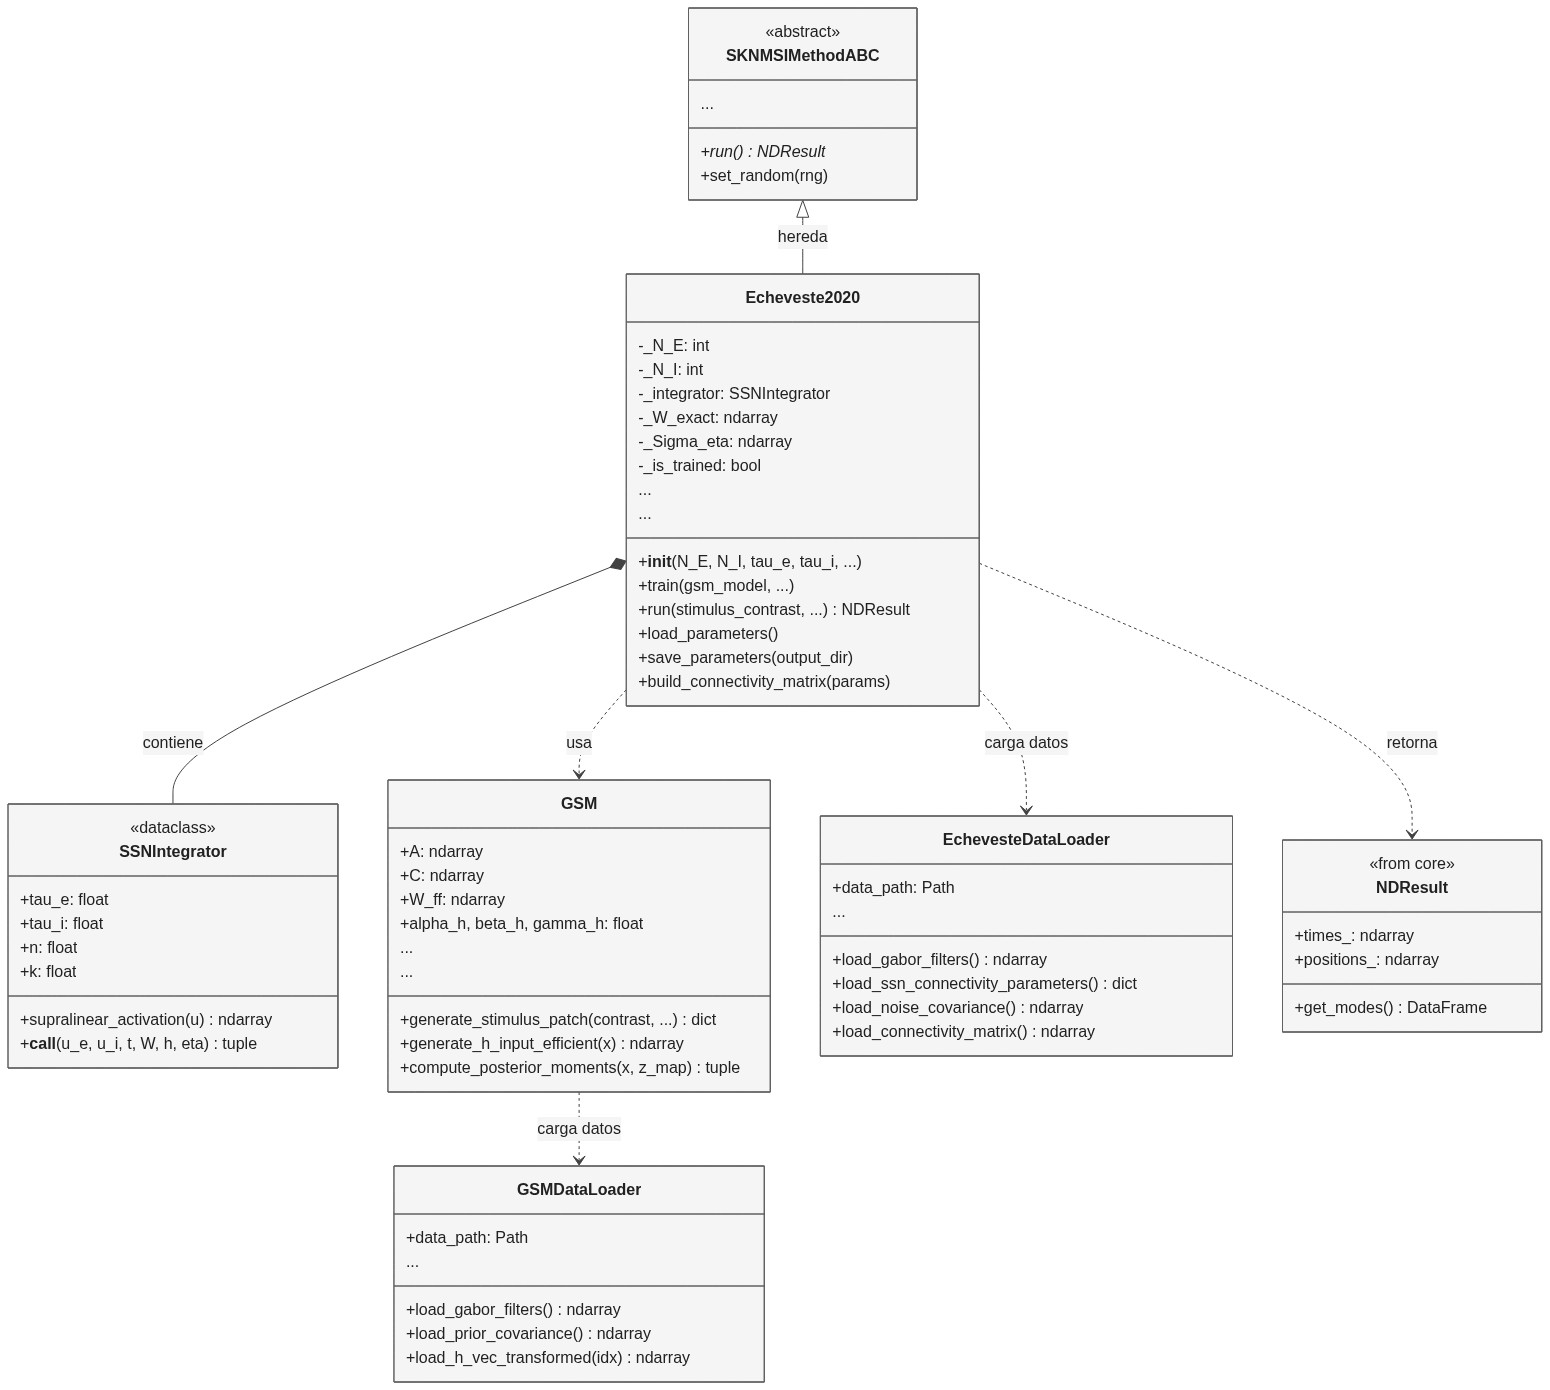
\includegraphics[width=1.3\textwidth]{10_apendice/figures/01_class_diagram_simplified.png}
    }
    \caption{
        Diagrama de clases UML detallado de la implementación Echeveste2020. Se observa la herencia desde la clase base abstracta \texttt{SKNMSIMethodABC}, la composición del integrador \texttt{SSNIntegrator} como dataclass, las dependencias con el modelo generativo \acrshort{GSM} y los cargadores de datos (\texttt{EchevesteDataLoader}, \texttt{GSMDataLoader}) para la configuración de la red. Los parámetros de los modelos están simplificados indicándolo con ``...''.
    }
    \label{fig:class-diagram}
\end{figure}

%=============================================================================
%=============================================================================

\clearpage
\newgeometry{margin=0cm}

\begin{figure}[p]
    \centering
    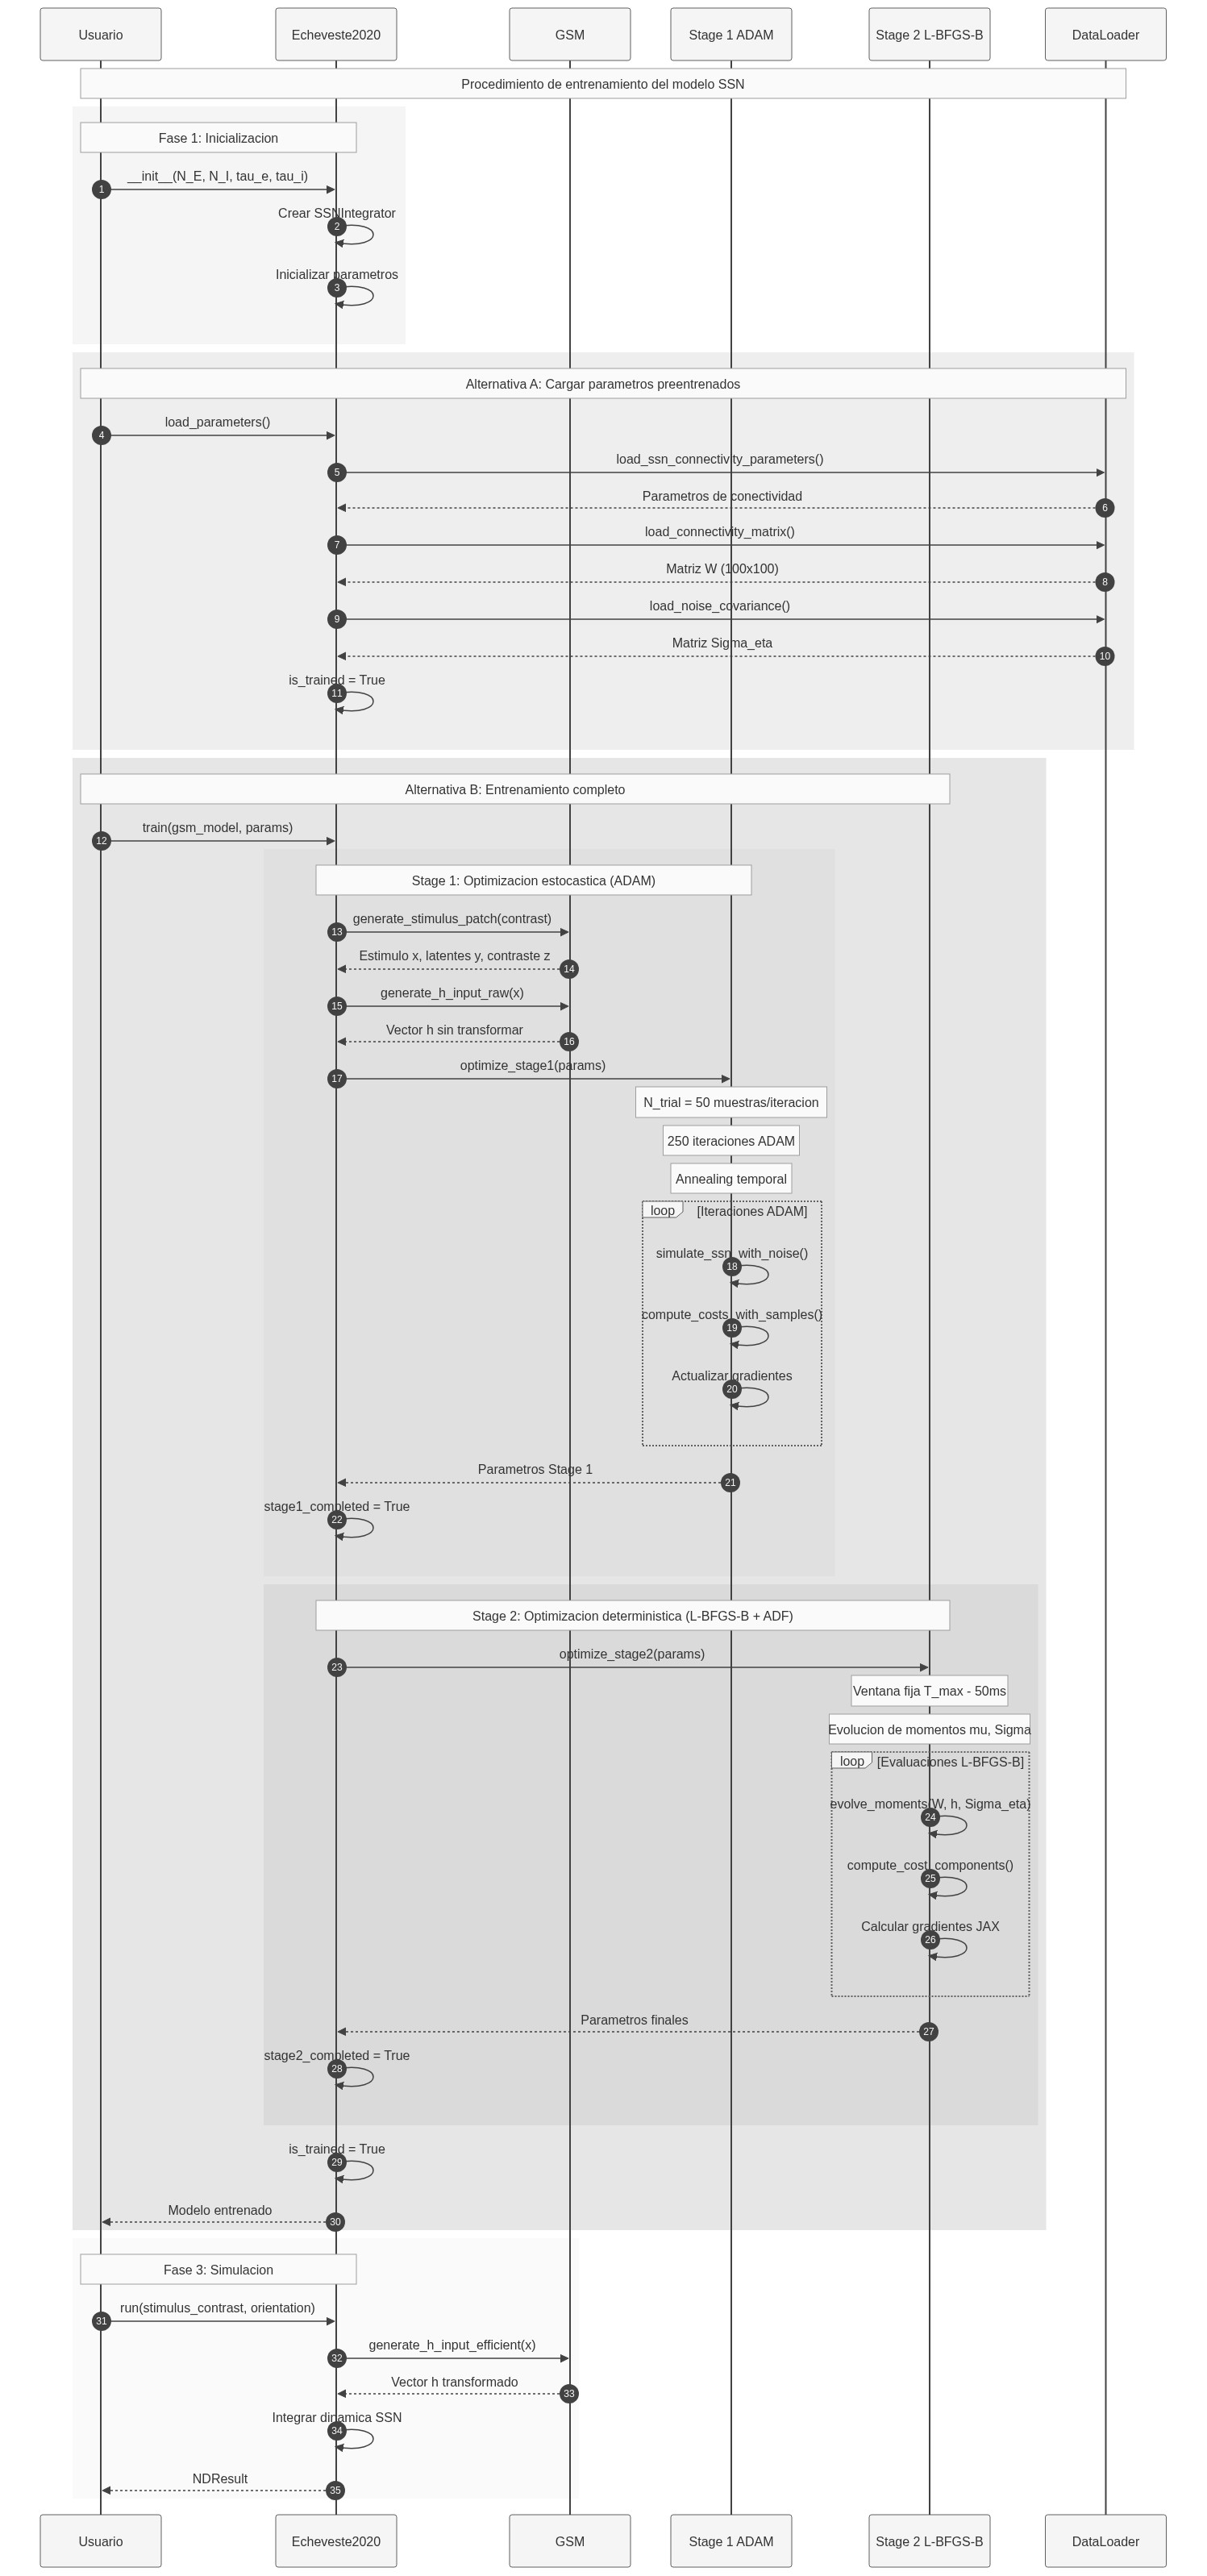
\includegraphics[width=0.9\paperwidth,height=0.8\paperheight,keepaspectratio]{10_apendice/figures/04_sequence_training_formal.png}
    \caption{Diagrama de secuencia completo del proceso de entrenamiento y validación.}
    \label{fig:sequence-training-full}
\end{figure}

\restoregeometry
\clearpage

%=============================================================================
%=============================================================================

\begin{figure}[H]
    \centering
    \makebox[\textwidth][c]{
        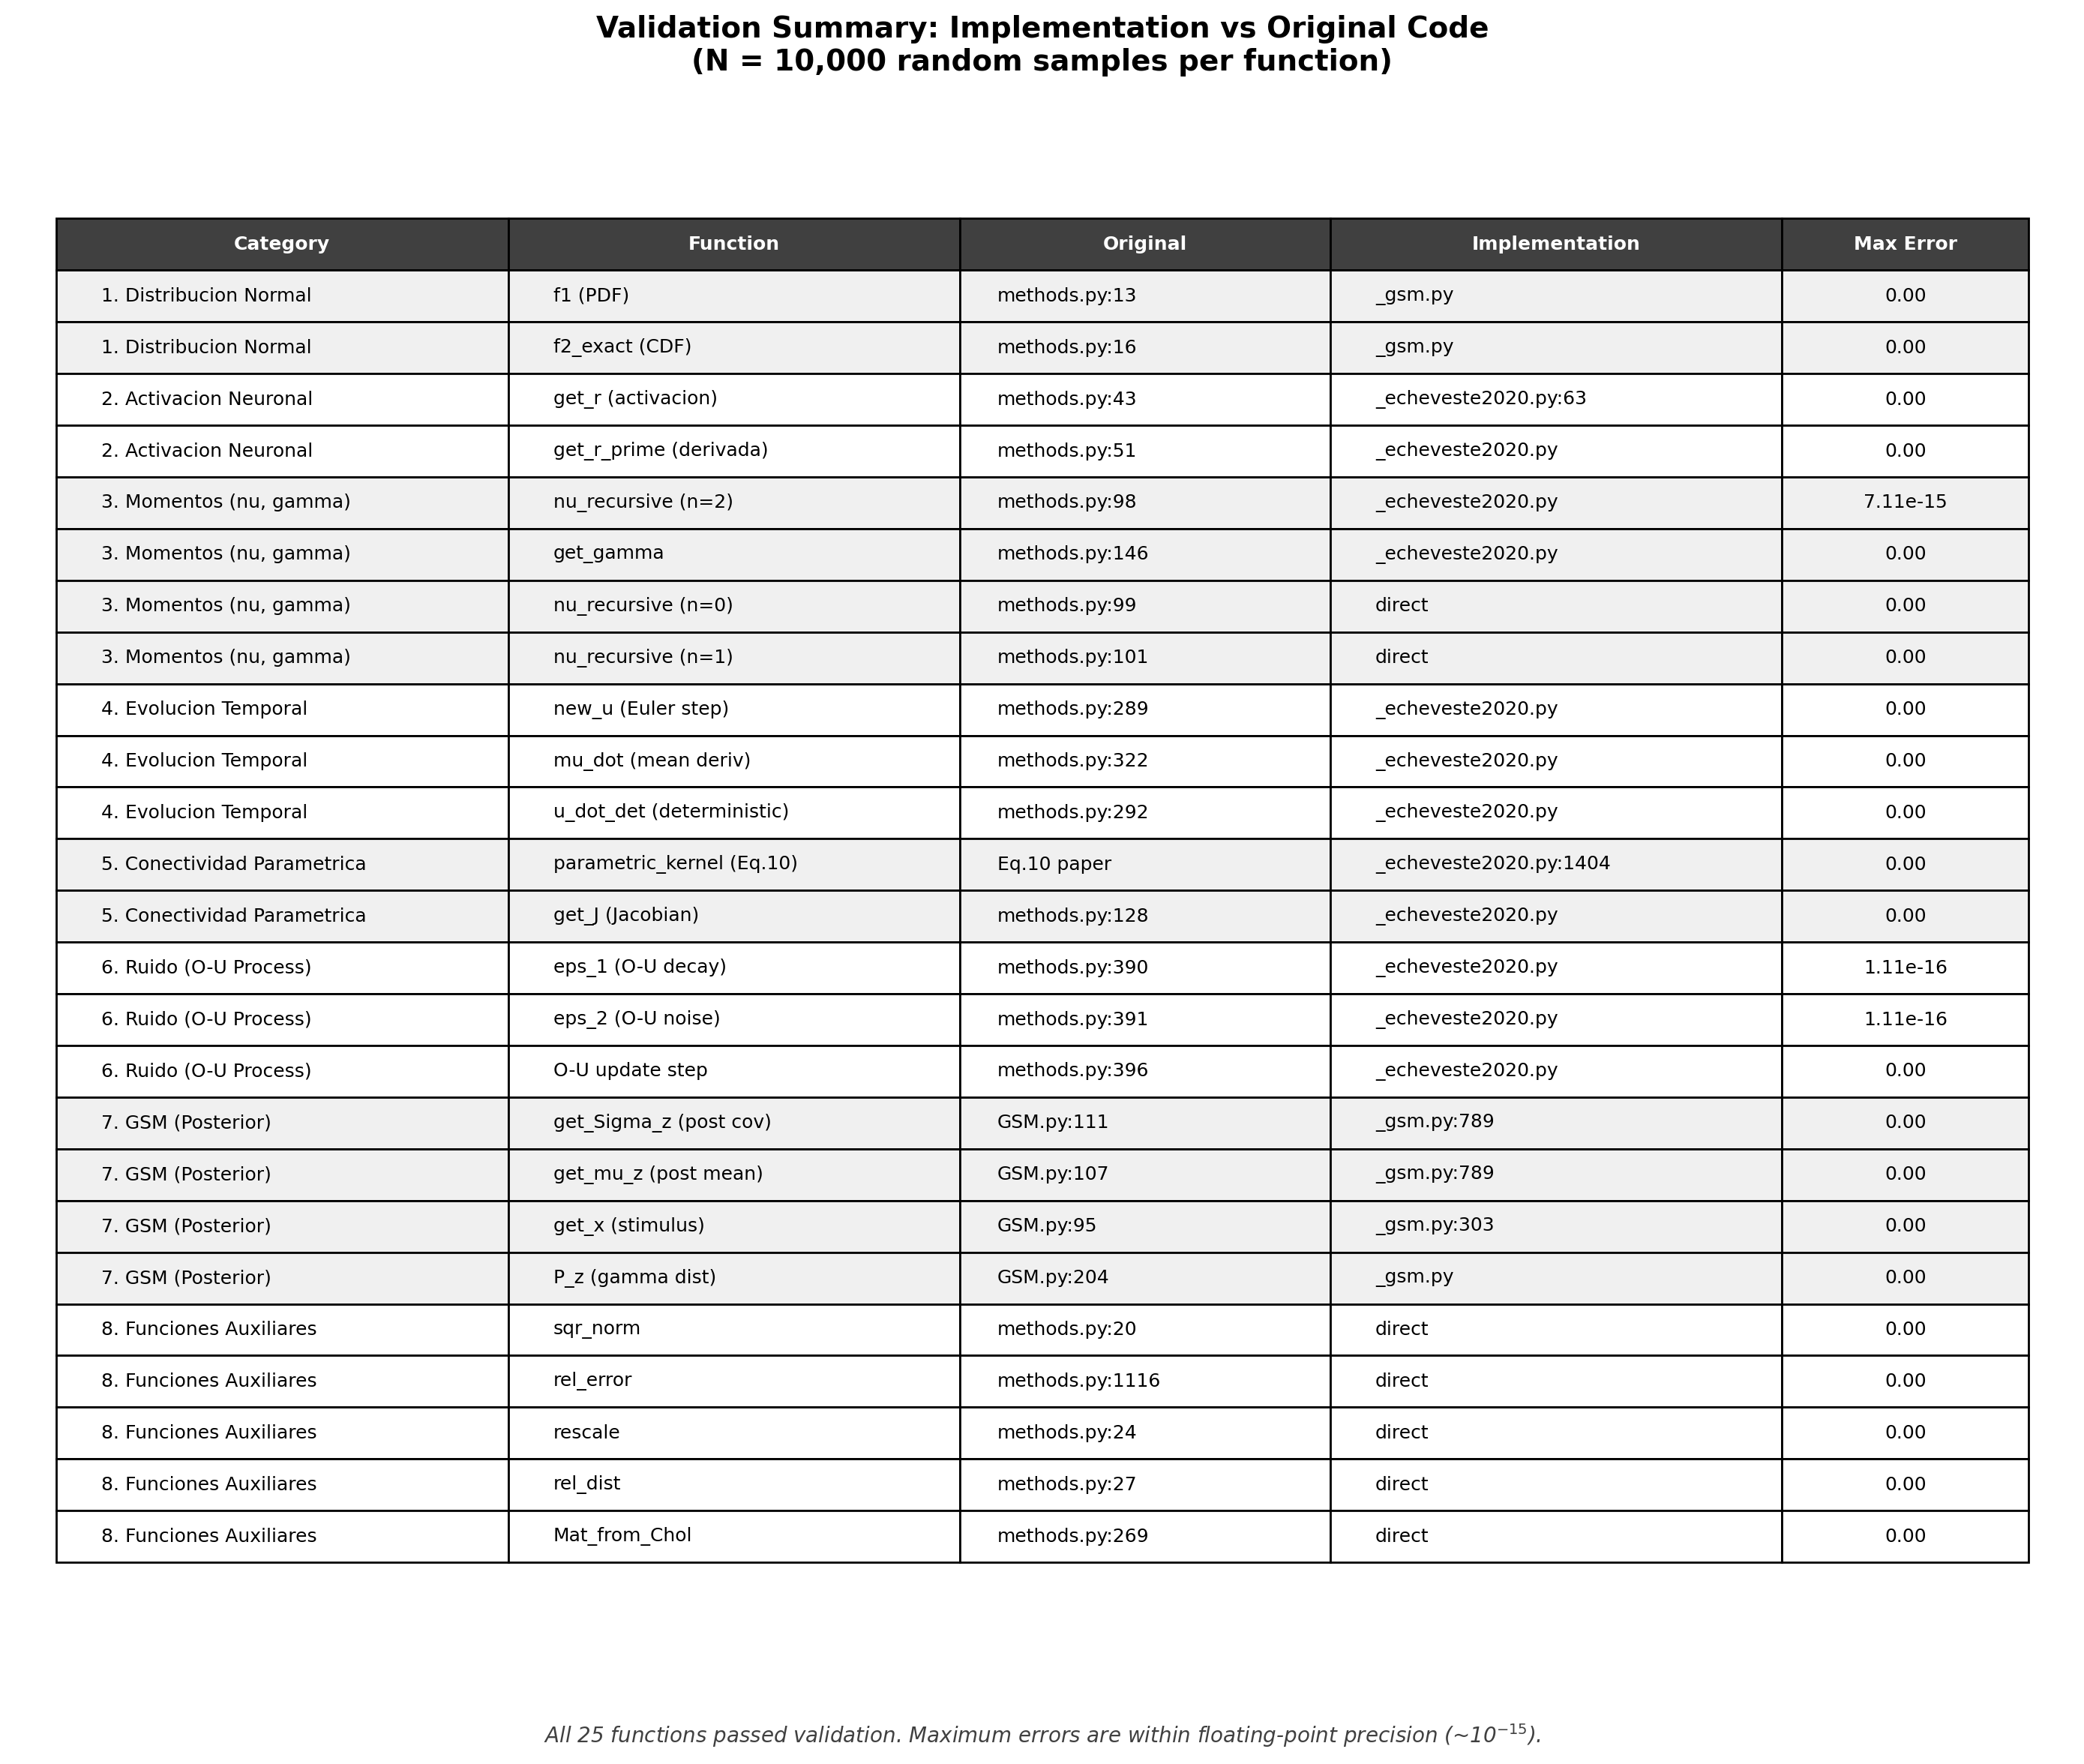
\includegraphics[width=1.3\textwidth]{10_apendice/figures/comprehensive_validation_formal.png}
    }
    \caption{
        Resumen completo de validación función por función. La tabla muestra las 25 funciones validadas, organizadas por categoría, con referencias a las líneas de código específicas tanto en el repositorio original (\texttt{methods.py}, \texttt{GSM.py}) como en nuestra implementación (\texttt{\_echeveste2020.py}, \texttt{\_gsm.py}). Todos los errores máximos están en el orden de la precisión de punto flotante ($\sim 10^{-15}$), confirmando equivalencia numérica exacta.
    }
    \label{fig:function-validation-complete}
\end{figure}
 \cleardoublepage

% BIBLIOGRAFIA ================================================================

% Usamos \phantomsection si usas hyperref para que el índice apunte al lugar correcto
\phantomsection
\addcontentsline{toc}{chapter}{Bibliografía}
\bibliographystyle{apalike}
\bibliography{tesis}

\clearpage 
\thispagestyle{empty} 

\vspace*{\fill} 

\begin{flushright}
    \large 
    \begin{CJK}{UTF8}{min} % 'min' es para la fuente Mincho (clásica japonesa)
        情報量、 それだけだ。
    \end{CJK}
\end{flushright}

\captionsetup[code]{skip=15pt}

\vspace{2cm} 
\clearpage
\end{document}
